\documentclass[twoside]{book}

% Packages required by doxygen
\usepackage{calc}
\usepackage{doxygen}
\usepackage{graphicx}
\usepackage[utf8]{inputenc}
\usepackage{makeidx}
\usepackage{multicol}
\usepackage{multirow}
\usepackage{fixltx2e}
\PassOptionsToPackage{warn}{textcomp}
\usepackage{textcomp}
\usepackage[nointegrals]{wasysym}
\usepackage[table]{xcolor}

% NLS support packages
\usepackage[french]{babel}

% Font selection
\usepackage[T1]{fontenc}
\usepackage{mathptmx}
\usepackage[scaled=.90]{helvet}
\usepackage{courier}
\usepackage{amssymb}
\usepackage{sectsty}
\renewcommand{\familydefault}{\sfdefault}
\allsectionsfont{%
  \fontseries{bc}\selectfont%
  \color{darkgray}%
}
\renewcommand{\DoxyLabelFont}{%
  \fontseries{bc}\selectfont%
  \color{darkgray}%
}
\newcommand{\+}{\discretionary{\mbox{\scriptsize$\hookleftarrow$}}{}{}}

% Page & text layout
\usepackage{geometry}
\geometry{%
  a4paper,%
  top=2.5cm,%
  bottom=2.5cm,%
  left=2.5cm,%
  right=2.5cm%
}
\tolerance=750
\hfuzz=15pt
\hbadness=750
\setlength{\emergencystretch}{15pt}
\setlength{\parindent}{0cm}
\setlength{\parskip}{0.2cm}
\makeatletter
\renewcommand{\paragraph}{%
  \@startsection{paragraph}{4}{0ex}{-1.0ex}{1.0ex}{%
    \normalfont\normalsize\bfseries\SS@parafont%
  }%
}
\renewcommand{\subparagraph}{%
  \@startsection{subparagraph}{5}{0ex}{-1.0ex}{1.0ex}{%
    \normalfont\normalsize\bfseries\SS@subparafont%
  }%
}
\makeatother

% Headers & footers
\usepackage{fancyhdr}
\pagestyle{fancyplain}
\fancyhead[LE]{\fancyplain{}{\bfseries\thepage}}
\fancyhead[CE]{\fancyplain{}{}}
\fancyhead[RE]{\fancyplain{}{\bfseries\leftmark}}
\fancyhead[LO]{\fancyplain{}{\bfseries\rightmark}}
\fancyhead[CO]{\fancyplain{}{}}
\fancyhead[RO]{\fancyplain{}{\bfseries\thepage}}
\fancyfoot[LE]{\fancyplain{}{}}
\fancyfoot[CE]{\fancyplain{}{}}
\fancyfoot[RE]{\fancyplain{}{\bfseries\scriptsize Généré le Lundi 2 Juin 2014 17\+:01\+:07 pour Castle par Doxygen }}
\fancyfoot[LO]{\fancyplain{}{\bfseries\scriptsize Généré le Lundi 2 Juin 2014 17\+:01\+:07 pour Castle par Doxygen }}
\fancyfoot[CO]{\fancyplain{}{}}
\fancyfoot[RO]{\fancyplain{}{}}
\renewcommand{\footrulewidth}{0.4pt}
\renewcommand{\chaptermark}[1]{%
  \markboth{#1}{}%
}
\renewcommand{\sectionmark}[1]{%
  \markright{\thesection\ #1}%
}

% Indices & bibliography
\usepackage{natbib}
\usepackage[titles]{tocloft}
\setcounter{tocdepth}{3}
\setcounter{secnumdepth}{5}
\makeindex

% Hyperlinks (required, but should be loaded last)
\usepackage{ifpdf}
\ifpdf
  \usepackage[pdftex,pagebackref=true]{hyperref}
\else
  \usepackage[ps2pdf,pagebackref=true]{hyperref}
\fi
\hypersetup{%
  colorlinks=true,%
  linkcolor=blue,%
  citecolor=blue,%
  unicode%
}

% Custom commands
\newcommand{\clearemptydoublepage}{%
  \newpage{\pagestyle{empty}\cleardoublepage}%
}


%===== C O N T E N T S =====

\begin{document}

% Titlepage & ToC
\hypersetup{pageanchor=false,
             bookmarks=true,
             bookmarksnumbered=true,
             pdfencoding=unicode
            }
\pagenumbering{roman}
\begin{titlepage}
\vspace*{7cm}
\begin{center}%
{\Large Castle }\\
\vspace*{1cm}
{\large Généré par Doxygen 1.8.7}\\
\vspace*{0.5cm}
{\small Lundi 2 Juin 2014 17:01:07}\\
\end{center}
\end{titlepage}
\clearemptydoublepage
\tableofcontents
\clearemptydoublepage
\pagenumbering{arabic}
\hypersetup{pageanchor=true}

%--- Begin generated contents ---
\chapter{Liste des choses à faire}
\label{todo}
\hypertarget{todo}{}

\begin{DoxyRefList}
\item[\label{todo__todo000001}%
\hypertarget{todo__todo000001}{}%
Class \hyperlink{class_light}{Light} ]attenuation de la lumière par lumière et plus globale  
\item[\label{todo__todo000003}%
\hypertarget{todo__todo000003}{}%
Member \hyperlink{class_light_a985e67a0b88ba49ec8da5d5b205d06ed}{Light\+:\+:set\+Number} (char num)]désactiver la lumière dans l'ancien slot  
\item[\label{todo__todo000002}%
\hypertarget{todo__todo000002}{}%
Member \hyperlink{class_light_ad0e59fad13bb6cfadc25b2c477e9ddc7}{Light\+:\+:$\sim$\+Light} ()]Vérifier que la lumière est désactivée dans tout les shader  
\item[\label{todo__todo000004}%
\hypertarget{todo__todo000004}{}%
Member \hyperlink{class_material_a2c19452d71f54075df8f5405b03129f4}{Material\+:\+:$\sim$\+Material} ()]Gérer libération de la texture quand plus utilisée 
\end{DoxyRefList}
\chapter{Index hiérarchique}
\section{Class Hierarchy}
This inheritance list is sorted roughly, but not completely, alphabetically\+:\begin{DoxyCompactList}
\item \contentsline{section}{Hitbox}{\pageref{class_hitbox}}{}
\begin{DoxyCompactList}
\item \contentsline{section}{Camera}{\pageref{class_camera}}{}
\item \contentsline{section}{Objet}{\pageref{class_objet}}{}
\begin{DoxyCompactList}
\item \contentsline{section}{Cube}{\pageref{class_cube}}{}
\item \contentsline{section}{Donuts}{\pageref{class_donuts}}{}
\item \contentsline{section}{Mesh}{\pageref{class_mesh}}{}
\item \contentsline{section}{Node}{\pageref{class_node}}{}
\item \contentsline{section}{Piece}{\pageref{class_piece}}{}
\item \contentsline{section}{Plan}{\pageref{class_plan}}{}
\item \contentsline{section}{Sphere}{\pageref{class_sphere}}{}
\end{DoxyCompactList}
\item \contentsline{section}{Scene}{\pageref{class_scene}}{}
\end{DoxyCompactList}
\item \contentsline{section}{mat3}{\pageref{structmat3}}{}
\item \contentsline{section}{mat4}{\pageref{structmat4}}{}
\item \contentsline{section}{Mesh\+:\+:Mesh\+Info}{\pageref{struct_mesh_1_1_mesh_info}}{}
\item Q\+Dock\+Widget\begin{DoxyCompactList}
\item \contentsline{section}{Mondock}{\pageref{class_mondock}}{}
\end{DoxyCompactList}
\item Q\+G\+L\+Widget\begin{DoxyCompactList}
\item \contentsline{section}{My\+Open\+G\+L\+Widget}{\pageref{class_my_open_g_l_widget}}{}
\end{DoxyCompactList}
\item Q\+Main\+Window\begin{DoxyCompactList}
\item \contentsline{section}{Main\+Window}{\pageref{class_main_window}}{}
\end{DoxyCompactList}
\item Q\+Open\+G\+L\+Functions\+\_\+3\+\_\+2\+\_\+\+Core\begin{DoxyCompactList}
\item \contentsline{section}{Light}{\pageref{class_light}}{}
\item \contentsline{section}{Material}{\pageref{class_material}}{}
\item \contentsline{section}{My\+Open\+G\+L\+Widget}{\pageref{class_my_open_g_l_widget}}{}
\item \contentsline{section}{Objet}{\pageref{class_objet}}{}
\item \contentsline{section}{Scene}{\pageref{class_scene}}{}
\end{DoxyCompactList}
\item \contentsline{section}{vec2}{\pageref{structvec2}}{}
\item \contentsline{section}{vec3}{\pageref{structvec3}}{}
\item \contentsline{section}{vec4}{\pageref{structvec4}}{}
\end{DoxyCompactList}

\chapter{Index des classes}
\section{Liste des classes}
Liste des classes, structures, unions et interfaces avec une brève description \+:\begin{DoxyCompactList}
\item\contentsline{section}{\hyperlink{class_camera}{Camera} \\*\hyperlink{class_camera}{Camera} pour \hyperlink{class_scene}{Scene} }{\pageref{class_camera}}{}
\item\contentsline{section}{\hyperlink{class_cube}{Cube} \\*Primitive cube }{\pageref{class_cube}}{}
\item\contentsline{section}{\hyperlink{class_donuts}{Donuts} \\*Primitive tore }{\pageref{class_donuts}}{}
\item\contentsline{section}{\hyperlink{class_light}{Light} \\*Lumière pour la \hyperlink{class_scene}{Scene} }{\pageref{class_light}}{}
\item\contentsline{section}{\hyperlink{class_main_window}{Main\+Window} }{\pageref{class_main_window}}{}
\item\contentsline{section}{\hyperlink{structmat3}{mat3} }{\pageref{structmat3}}{}
\item\contentsline{section}{\hyperlink{structmat4}{mat4} }{\pageref{structmat4}}{}
\item\contentsline{section}{\hyperlink{class_material}{Material} \\*Matériaux pour la \hyperlink{class_scene}{Scene} }{\pageref{class_material}}{}
\item\contentsline{section}{\hyperlink{class_mesh}{Mesh} \\*Charge un modèle 3\+D }{\pageref{class_mesh}}{}
\item\contentsline{section}{\hyperlink{struct_mesh_1_1_mesh_info}{Mesh\+::\+Mesh\+Info} }{\pageref{struct_mesh_1_1_mesh_info}}{}
\item\contentsline{section}{\hyperlink{class_mondock}{Mondock} }{\pageref{class_mondock}}{}
\item\contentsline{section}{\hyperlink{class_my_open_g_l_widget}{My\+Open\+G\+L\+Widget} }{\pageref{class_my_open_g_l_widget}}{}
\item\contentsline{section}{\hyperlink{class_node}{Node} \\*Contient un node de modèle 3\+D }{\pageref{class_node}}{}
\item\contentsline{section}{\hyperlink{class_objet}{Objet} \\*Classe de base affichable }{\pageref{class_objet}}{}
\item\contentsline{section}{\hyperlink{class_piece}{Piece} \\*Pièce, contient un ensemble d'objet qu'elle contient }{\pageref{class_piece}}{}
\item\contentsline{section}{\hyperlink{class_plan}{Plan} \\*\hyperlink{class_plan}{Plan} utilisé par la \hyperlink{class_piece}{Piece} }{\pageref{class_plan}}{}
\item\contentsline{section}{\hyperlink{class_scene}{Scene} \\*Classe principale }{\pageref{class_scene}}{}
\item\contentsline{section}{\hyperlink{class_sphere}{Sphere} \\*Primitive tore }{\pageref{class_sphere}}{}
\item\contentsline{section}{\hyperlink{structvec2}{vec2} }{\pageref{structvec2}}{}
\item\contentsline{section}{\hyperlink{structvec3}{vec3} }{\pageref{structvec3}}{}
\item\contentsline{section}{\hyperlink{structvec4}{vec4} }{\pageref{structvec4}}{}
\end{DoxyCompactList}

\chapter{Index des fichiers}
\section{File List}
Here is a list of all files with brief descriptions\+:\begin{DoxyCompactList}
\item\contentsline{section}{\hyperlink{camera_8cpp}{camera.\+cpp} }{\pageref{camera_8cpp}}{}
\item\contentsline{section}{\hyperlink{camera_8hpp}{camera.\+hpp} }{\pageref{camera_8hpp}}{}
\item\contentsline{section}{\hyperlink{helper_8cpp}{helper.\+cpp} }{\pageref{helper_8cpp}}{}
\item\contentsline{section}{\hyperlink{helper_8hpp}{helper.\+hpp} }{\pageref{helper_8hpp}}{}
\item\contentsline{section}{\hyperlink{main_8cpp}{main.\+cpp} }{\pageref{main_8cpp}}{}
\item\contentsline{section}{gui/\hyperlink{mainwindows_8cpp}{mainwindows.\+cpp} }{\pageref{mainwindows_8cpp}}{}
\item\contentsline{section}{gui/\hyperlink{mainwindows_8hpp}{mainwindows.\+hpp} }{\pageref{mainwindows_8hpp}}{}
\item\contentsline{section}{gui/\hyperlink{mondock_8cpp}{mondock.\+cpp} }{\pageref{mondock_8cpp}}{}
\item\contentsline{section}{gui/\hyperlink{mondock_8hpp}{mondock.\+hpp} }{\pageref{mondock_8hpp}}{}
\item\contentsline{section}{gui/\hyperlink{_my_open_g_l_widget_8cpp}{My\+Open\+G\+L\+Widget.\+cpp} }{\pageref{_my_open_g_l_widget_8cpp}}{}
\item\contentsline{section}{gui/\hyperlink{_my_open_g_l_widget_8hpp}{My\+Open\+G\+L\+Widget.\+hpp} }{\pageref{_my_open_g_l_widget_8hpp}}{}
\item\contentsline{section}{objets/\hyperlink{cube_8cpp}{cube.\+cpp} }{\pageref{cube_8cpp}}{}
\item\contentsline{section}{objets/\hyperlink{cube_8hpp}{cube.\+hpp} }{\pageref{cube_8hpp}}{}
\item\contentsline{section}{objets/\hyperlink{donuts_8cpp}{donuts.\+cpp} }{\pageref{donuts_8cpp}}{}
\item\contentsline{section}{objets/\hyperlink{donuts_8hpp}{donuts.\+hpp} }{\pageref{donuts_8hpp}}{}
\item\contentsline{section}{objets/\hyperlink{mesh_8cpp}{mesh.\+cpp} }{\pageref{mesh_8cpp}}{}
\item\contentsline{section}{objets/\hyperlink{mesh_8hpp}{mesh.\+hpp} }{\pageref{mesh_8hpp}}{}
\item\contentsline{section}{objets/\hyperlink{node_8cpp}{node.\+cpp} }{\pageref{node_8cpp}}{}
\item\contentsline{section}{objets/\hyperlink{node_8hpp}{node.\+hpp} }{\pageref{node_8hpp}}{}
\item\contentsline{section}{objets/\hyperlink{objet_8cpp}{objet.\+cpp} }{\pageref{objet_8cpp}}{}
\item\contentsline{section}{objets/\hyperlink{objet_8hpp}{objet.\+hpp} }{\pageref{objet_8hpp}}{}
\item\contentsline{section}{objets/\hyperlink{plan_8cpp}{plan.\+cpp} }{\pageref{plan_8cpp}}{}
\item\contentsline{section}{objets/\hyperlink{plan_8hpp}{plan.\+hpp} }{\pageref{plan_8hpp}}{}
\item\contentsline{section}{objets/\hyperlink{sphere_8cpp}{sphere.\+cpp} }{\pageref{sphere_8cpp}}{}
\item\contentsline{section}{objets/\hyperlink{sphere_8hpp}{sphere.\+hpp} }{\pageref{sphere_8hpp}}{}
\item\contentsline{section}{scene/\hyperlink{light_8cpp}{light.\+cpp} }{\pageref{light_8cpp}}{}
\item\contentsline{section}{scene/\hyperlink{light_8hpp}{light.\+hpp} }{\pageref{light_8hpp}}{}
\item\contentsline{section}{scene/\hyperlink{material_8cpp}{material.\+cpp} }{\pageref{material_8cpp}}{}
\item\contentsline{section}{scene/\hyperlink{material_8hpp}{material.\+hpp} }{\pageref{material_8hpp}}{}
\item\contentsline{section}{scene/\hyperlink{piece_8cpp}{piece.\+cpp} }{\pageref{piece_8cpp}}{}
\item\contentsline{section}{scene/\hyperlink{piece_8hpp}{piece.\+hpp} }{\pageref{piece_8hpp}}{}
\item\contentsline{section}{scene/\hyperlink{scene_8cpp}{scene.\+cpp} }{\pageref{scene_8cpp}}{}
\item\contentsline{section}{scene/\hyperlink{scene_8hpp}{scene.\+hpp} }{\pageref{scene_8hpp}}{}
\end{DoxyCompactList}

\chapter{Documentation des classes}
\hypertarget{class_camera}{\section{Référence de la classe Camera}
\label{class_camera}\index{Camera@{Camera}}
}


\hyperlink{class_camera}{Camera} pour \hyperlink{class_scene}{Scene}.  




{\ttfamily \#include $<$camera.\+hpp$>$}



Graphe de collaboration de Camera\+:
\nopagebreak
\begin{figure}[H]
\begin{center}
\leavevmode
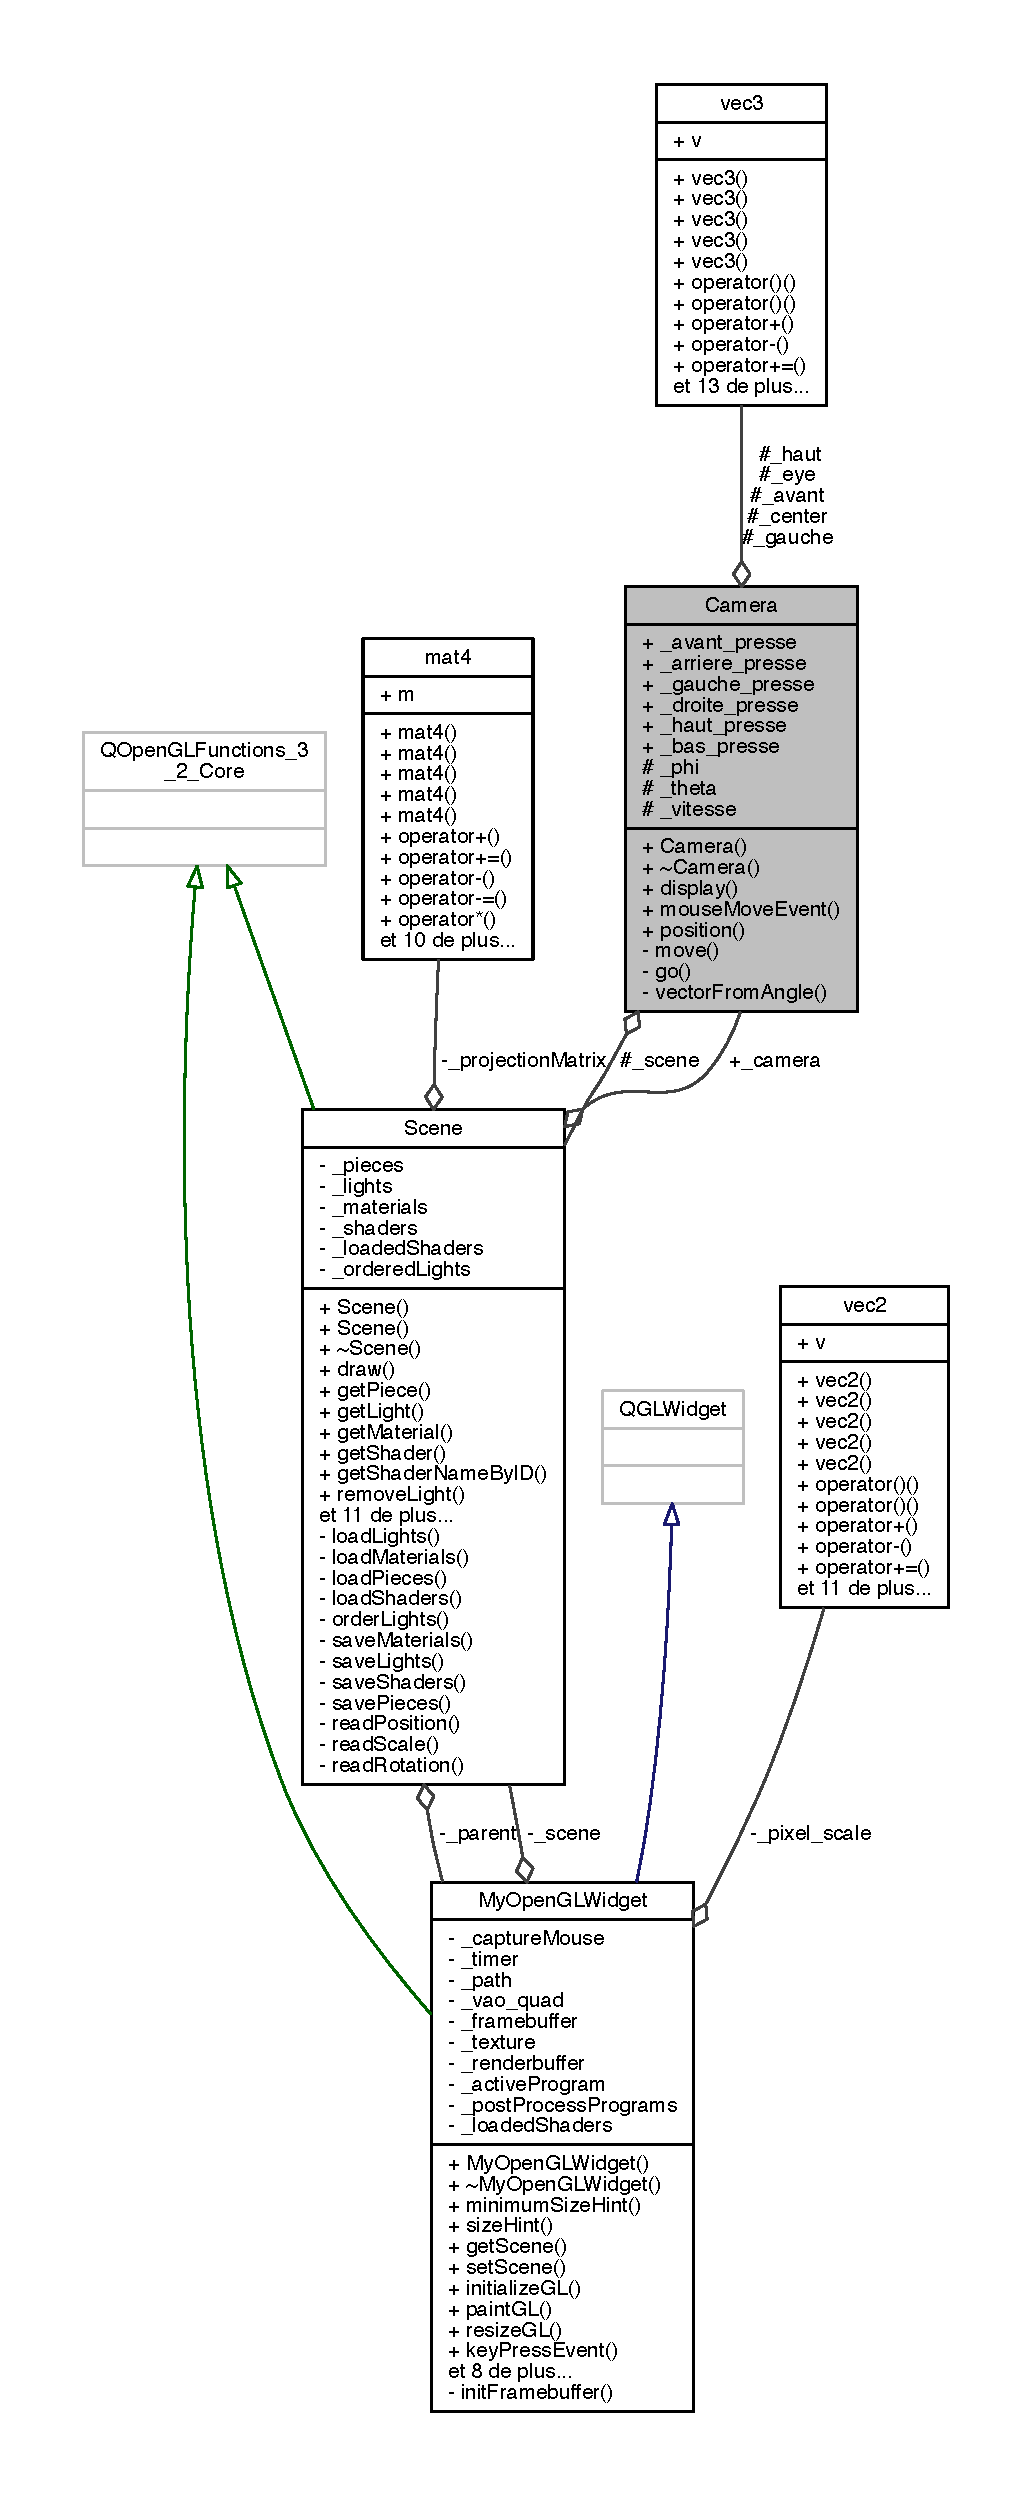
\includegraphics[height=550pt]{class_camera__coll__graph}
\end{center}
\end{figure}
\subsection*{Fonctions membres publiques}
\begin{DoxyCompactItemize}
\item 
\hyperlink{class_camera_a1a8ac754efe577c8abbc1e19cc8bca25}{Camera} (\hyperlink{class_scene}{Scene} $\ast$scene=N\+U\+L\+L, float eye\+X=0.\+0f, float eye\+Y=0.\+0f, float eye\+Z=0.\+0f)
\begin{DoxyCompactList}\small\item\em Constructeur. \end{DoxyCompactList}\item 
\hyperlink{class_camera_ad1897942d0ccf91052386388a497349f}{$\sim$\+Camera} ()
\begin{DoxyCompactList}\small\item\em Destructeur. \end{DoxyCompactList}\item 
void \hyperlink{class_camera_adbfdac30f082ddea86183c1c31493946}{display} ()
\begin{DoxyCompactList}\small\item\em Actualise la caméra. \end{DoxyCompactList}\item 
void \hyperlink{class_camera_a22aaf20b581d402e5c3952655b830c0f}{mouse\+Move\+Event} (int x, int y, int width, int height)
\begin{DoxyCompactList}\small\item\em Fonction de déplacement de la caméra à la souris. \end{DoxyCompactList}\item 
const \hyperlink{structvec3}{vec3} \& \hyperlink{class_camera_ad42b0114b12a48474ae6c8be1c44e7bb}{position} () const 
\begin{DoxyCompactList}\small\item\em Retourne la position de la caméra. \end{DoxyCompactList}\end{DoxyCompactItemize}
\subsection*{Attributs publics}
\begin{DoxyCompactItemize}
\item 
bool \hyperlink{class_camera_a4cab15e35a96fdcb2a8599fea13a9b8f}{\+\_\+avant\+\_\+presse}
\item 
bool \hyperlink{class_camera_a0ce12f74953fcd53192e48f8b4164e2e}{\+\_\+arriere\+\_\+presse}
\item 
bool \hyperlink{class_camera_ac2a5c37c4f9603a14e3616d6a75f7998}{\+\_\+gauche\+\_\+presse}
\item 
bool \hyperlink{class_camera_a61b2e438537b99ba1f0a97e5586b7f45}{\+\_\+droite\+\_\+presse}
\item 
bool \hyperlink{class_camera_a43b59b53cb182906d56e6e4d2c31139c}{\+\_\+haut\+\_\+presse}
\item 
bool \hyperlink{class_camera_aaba6828f97c9ef07b6b135a665bd3008}{\+\_\+bas\+\_\+presse}
\end{DoxyCompactItemize}
\subsection*{Attributs protégés}
\begin{DoxyCompactItemize}
\item 
\hyperlink{structvec3}{vec3} \hyperlink{class_camera_ad4c22c27bd247f4411c4166220ba6e82}{\+\_\+eye}
\item 
\hyperlink{structvec3}{vec3} \hyperlink{class_camera_ad80a82cbc81e6d8ba04c7cc1ac7ba0d7}{\+\_\+center}
\item 
float \hyperlink{class_camera_a288df53a3ff446ee4367ee47b8499fcd}{\+\_\+phi}
\item 
float \hyperlink{class_camera_aeb3c859c3c254c8296420451259e5629}{\+\_\+theta}
\item 
\hyperlink{structvec3}{vec3} \hyperlink{class_camera_ab7cf8c1eae6b2f35a20e8abd1f0570c9}{\+\_\+avant}
\item 
\hyperlink{structvec3}{vec3} \hyperlink{class_camera_aaf97dba7663b99065d8d508b589224de}{\+\_\+gauche}
\item 
\hyperlink{structvec3}{vec3} \hyperlink{class_camera_af860db197a7abbf0284df4e32a95a347}{\+\_\+haut}
\item 
float \hyperlink{class_camera_a9062fdde515a49bf8db963ac46be9942}{\+\_\+vitesse}
\item 
\hyperlink{class_scene}{Scene} $\ast$ \hyperlink{class_camera_a81ffb00eedbaefbfb755b0c13d42180a}{\+\_\+scene}
\end{DoxyCompactItemize}
\subsection*{Fonctions membres privées}
\begin{DoxyCompactItemize}
\item 
void \hyperlink{class_camera_a8414e6d74d3f6259fa5ea1f037e9d8bd}{move} ()
\begin{DoxyCompactList}\small\item\em Calcul le déplacement de la \hyperlink{class_camera}{Camera}. \end{DoxyCompactList}\item 
void \hyperlink{class_camera_abde0ff477fb0baea7515767dcd7a7cf7}{go} (float x, float y, float z)
\begin{DoxyCompactList}\small\item\em Déplace la caméra aux coordonnées données. \end{DoxyCompactList}\item 
void \hyperlink{class_camera_aa4e815462a964caa6b10804e33119cf2}{vector\+From\+Angle} ()
\begin{DoxyCompactList}\small\item\em Recalcul les vecteurs avant/côté pour le mouvement. \end{DoxyCompactList}\end{DoxyCompactItemize}


\subsection{Description détaillée}
\hyperlink{class_camera}{Camera} pour \hyperlink{class_scene}{Scene}. 

\subsection{Documentation des constructeurs et destructeur}
\hypertarget{class_camera_a1a8ac754efe577c8abbc1e19cc8bca25}{\index{Camera@{Camera}!Camera@{Camera}}
\index{Camera@{Camera}!Camera@{Camera}}
\subsubsection[{Camera}]{\setlength{\rightskip}{0pt plus 5cm}Camera\+::\+Camera (
\begin{DoxyParamCaption}
\item[{{\bf Scene} $\ast$}]{scene = {\ttfamily NULL}, }
\item[{float}]{eye\+X = {\ttfamily 0.0f}, }
\item[{float}]{eye\+Y = {\ttfamily 0.0f}, }
\item[{float}]{eye\+Z = {\ttfamily 0.0f}}
\end{DoxyParamCaption}
)}}\label{class_camera_a1a8ac754efe577c8abbc1e19cc8bca25}


Constructeur. 



Voici le graphe d'appel pour cette fonction \+:
\nopagebreak
\begin{figure}[H]
\begin{center}
\leavevmode
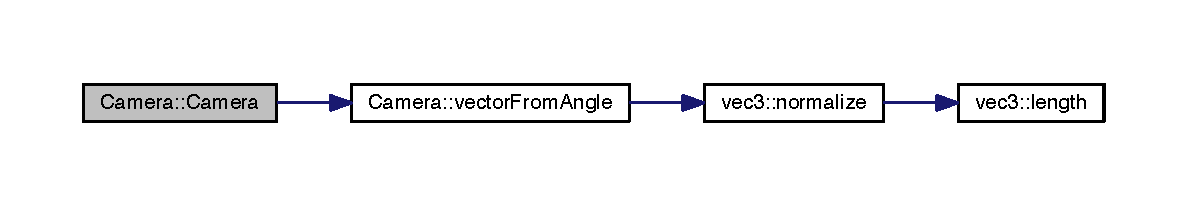
\includegraphics[width=350pt]{class_camera_a1a8ac754efe577c8abbc1e19cc8bca25_cgraph}
\end{center}
\end{figure}


\hypertarget{class_camera_ad1897942d0ccf91052386388a497349f}{\index{Camera@{Camera}!````~Camera@{$\sim$\+Camera}}
\index{````~Camera@{$\sim$\+Camera}!Camera@{Camera}}
\subsubsection[{$\sim$\+Camera}]{\setlength{\rightskip}{0pt plus 5cm}Camera\+::$\sim$\+Camera (
\begin{DoxyParamCaption}
{}
\end{DoxyParamCaption}
)\hspace{0.3cm}{\ttfamily [inline]}}}\label{class_camera_ad1897942d0ccf91052386388a497349f}


Destructeur. 



\subsection{Documentation des fonctions membres}
\hypertarget{class_camera_adbfdac30f082ddea86183c1c31493946}{\index{Camera@{Camera}!display@{display}}
\index{display@{display}!Camera@{Camera}}
\subsubsection[{display}]{\setlength{\rightskip}{0pt plus 5cm}void Camera\+::display (
\begin{DoxyParamCaption}
{}
\end{DoxyParamCaption}
)}}\label{class_camera_adbfdac30f082ddea86183c1c31493946}


Actualise la caméra. 

Met à jour la position de la caméra en fonction des booléens de déplacement et actualise la matrice view 

Voici le graphe d'appel pour cette fonction \+:
\nopagebreak
\begin{figure}[H]
\begin{center}
\leavevmode
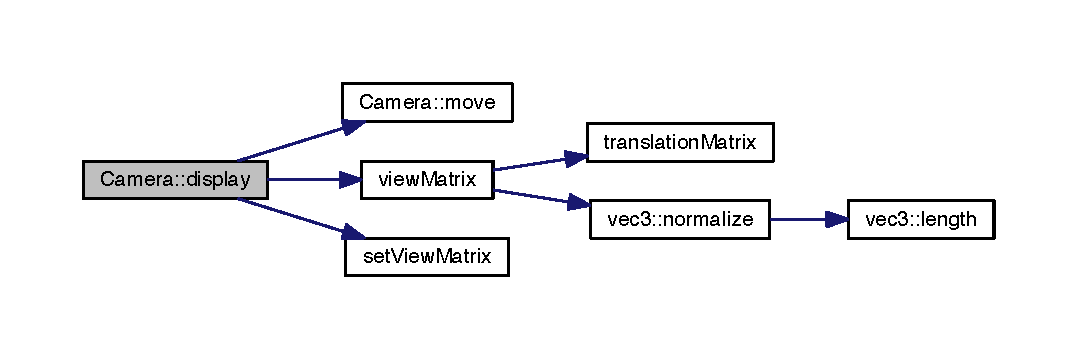
\includegraphics[width=350pt]{class_camera_adbfdac30f082ddea86183c1c31493946_cgraph}
\end{center}
\end{figure}




Voici le graphe des appelants de cette fonction \+:
\nopagebreak
\begin{figure}[H]
\begin{center}
\leavevmode
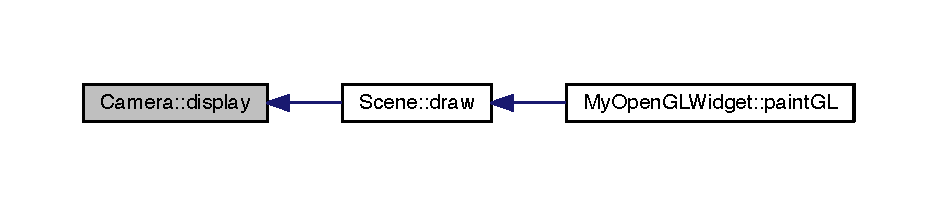
\includegraphics[width=350pt]{class_camera_adbfdac30f082ddea86183c1c31493946_icgraph}
\end{center}
\end{figure}


\hypertarget{class_camera_abde0ff477fb0baea7515767dcd7a7cf7}{\index{Camera@{Camera}!go@{go}}
\index{go@{go}!Camera@{Camera}}
\subsubsection[{go}]{\setlength{\rightskip}{0pt plus 5cm}void Camera\+::go (
\begin{DoxyParamCaption}
\item[{float}]{x, }
\item[{float}]{y, }
\item[{float}]{z}
\end{DoxyParamCaption}
)\hspace{0.3cm}{\ttfamily [private]}}}\label{class_camera_abde0ff477fb0baea7515767dcd7a7cf7}


Déplace la caméra aux coordonnées données. 

\hypertarget{class_camera_a22aaf20b581d402e5c3952655b830c0f}{\index{Camera@{Camera}!mouse\+Move\+Event@{mouse\+Move\+Event}}
\index{mouse\+Move\+Event@{mouse\+Move\+Event}!Camera@{Camera}}
\subsubsection[{mouse\+Move\+Event}]{\setlength{\rightskip}{0pt plus 5cm}void Camera\+::mouse\+Move\+Event (
\begin{DoxyParamCaption}
\item[{int}]{x, }
\item[{int}]{y, }
\item[{int}]{width, }
\item[{int}]{height}
\end{DoxyParamCaption}
)}}\label{class_camera_a22aaf20b581d402e5c3952655b830c0f}


Fonction de déplacement de la caméra à la souris. 


\begin{DoxyParams}{Paramètres}
{\em x} & position en X du curseur de la souris \\
\hline
{\em y} & position en Y du curseur de la souris \\
\hline
{\em width} & largeur de la fenêtre \\
\hline
{\em height} & hauteur de la fenêtre \\
\hline
\end{DoxyParams}


Voici le graphe d'appel pour cette fonction \+:
\nopagebreak
\begin{figure}[H]
\begin{center}
\leavevmode
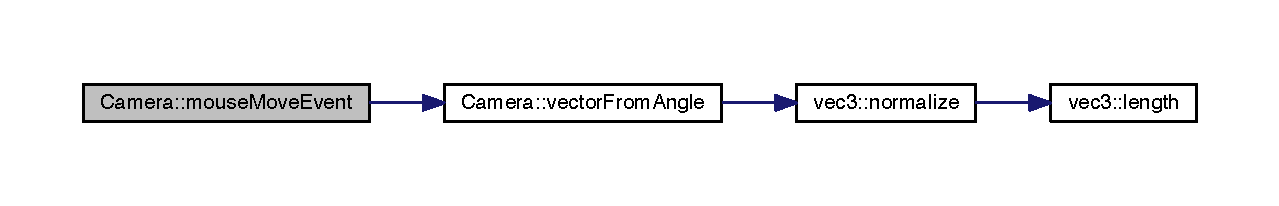
\includegraphics[width=350pt]{class_camera_a22aaf20b581d402e5c3952655b830c0f_cgraph}
\end{center}
\end{figure}




Voici le graphe des appelants de cette fonction \+:
\nopagebreak
\begin{figure}[H]
\begin{center}
\leavevmode
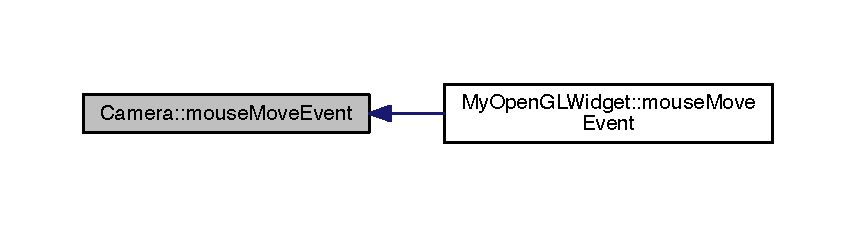
\includegraphics[width=350pt]{class_camera_a22aaf20b581d402e5c3952655b830c0f_icgraph}
\end{center}
\end{figure}


\hypertarget{class_camera_a8414e6d74d3f6259fa5ea1f037e9d8bd}{\index{Camera@{Camera}!move@{move}}
\index{move@{move}!Camera@{Camera}}
\subsubsection[{move}]{\setlength{\rightskip}{0pt plus 5cm}void Camera\+::move (
\begin{DoxyParamCaption}
{}
\end{DoxyParamCaption}
)\hspace{0.3cm}{\ttfamily [private]}}}\label{class_camera_a8414e6d74d3f6259fa5ea1f037e9d8bd}


Calcul le déplacement de la \hyperlink{class_camera}{Camera}. 



Voici le graphe des appelants de cette fonction \+:
\nopagebreak
\begin{figure}[H]
\begin{center}
\leavevmode
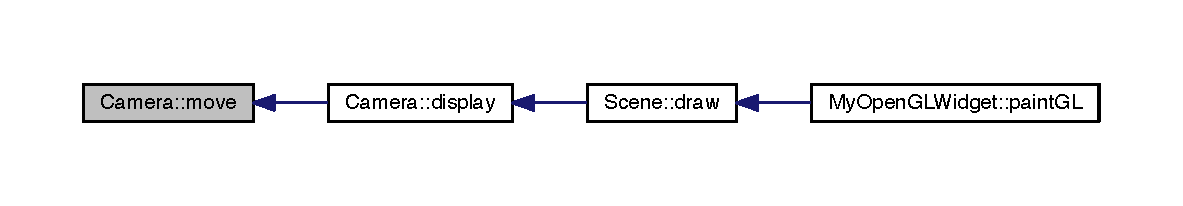
\includegraphics[width=350pt]{class_camera_a8414e6d74d3f6259fa5ea1f037e9d8bd_icgraph}
\end{center}
\end{figure}


\hypertarget{class_camera_ad42b0114b12a48474ae6c8be1c44e7bb}{\index{Camera@{Camera}!position@{position}}
\index{position@{position}!Camera@{Camera}}
\subsubsection[{position}]{\setlength{\rightskip}{0pt plus 5cm}const {\bf vec3}\& Camera\+::position (
\begin{DoxyParamCaption}
{}
\end{DoxyParamCaption}
) const\hspace{0.3cm}{\ttfamily [inline]}}}\label{class_camera_ad42b0114b12a48474ae6c8be1c44e7bb}


Retourne la position de la caméra. 



Voici le graphe des appelants de cette fonction \+:
\nopagebreak
\begin{figure}[H]
\begin{center}
\leavevmode
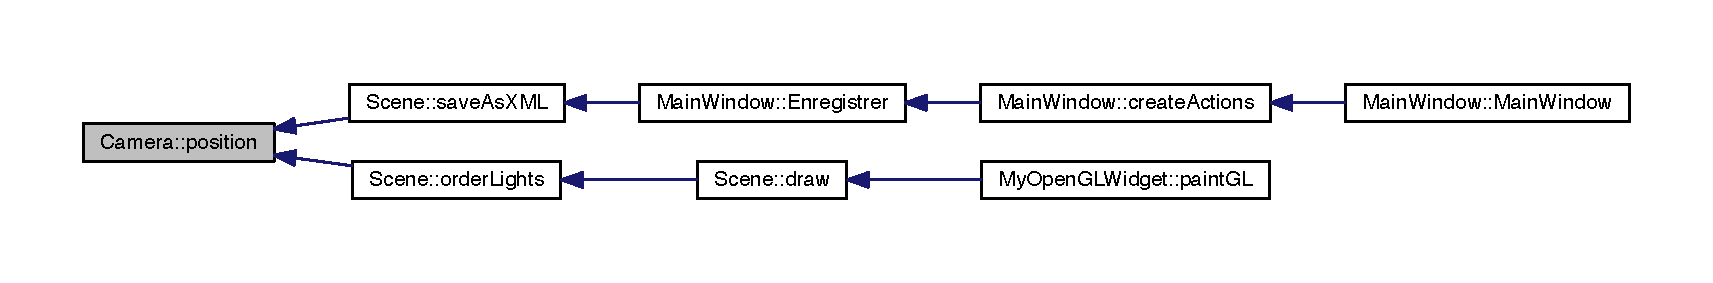
\includegraphics[width=350pt]{class_camera_ad42b0114b12a48474ae6c8be1c44e7bb_icgraph}
\end{center}
\end{figure}


\hypertarget{class_camera_aa4e815462a964caa6b10804e33119cf2}{\index{Camera@{Camera}!vector\+From\+Angle@{vector\+From\+Angle}}
\index{vector\+From\+Angle@{vector\+From\+Angle}!Camera@{Camera}}
\subsubsection[{vector\+From\+Angle}]{\setlength{\rightskip}{0pt plus 5cm}void Camera\+::vector\+From\+Angle (
\begin{DoxyParamCaption}
{}
\end{DoxyParamCaption}
)\hspace{0.3cm}{\ttfamily [private]}}}\label{class_camera_aa4e815462a964caa6b10804e33119cf2}


Recalcul les vecteurs avant/côté pour le mouvement. 



Voici le graphe d'appel pour cette fonction \+:
\nopagebreak
\begin{figure}[H]
\begin{center}
\leavevmode
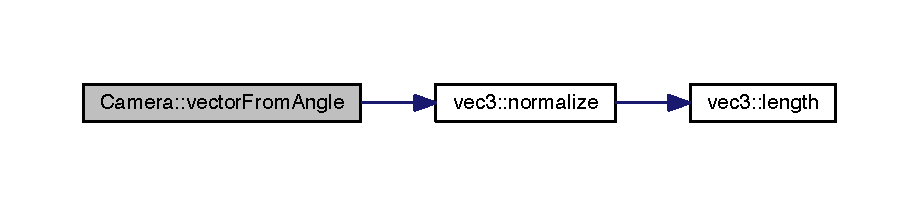
\includegraphics[width=350pt]{class_camera_aa4e815462a964caa6b10804e33119cf2_cgraph}
\end{center}
\end{figure}




Voici le graphe des appelants de cette fonction \+:
\nopagebreak
\begin{figure}[H]
\begin{center}
\leavevmode
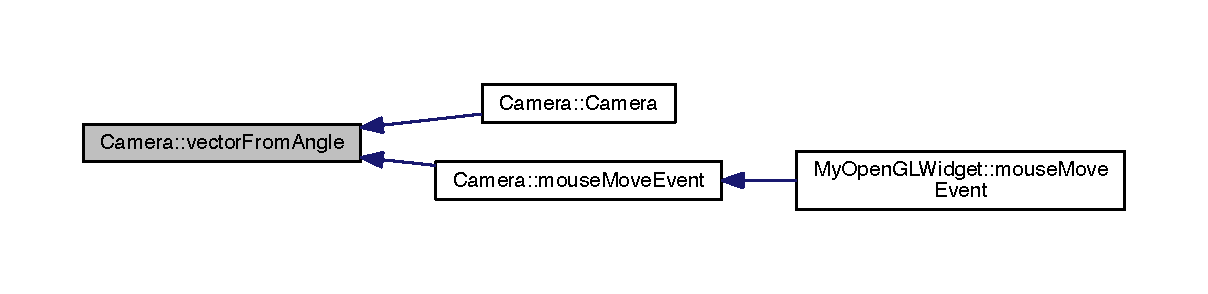
\includegraphics[width=350pt]{class_camera_aa4e815462a964caa6b10804e33119cf2_icgraph}
\end{center}
\end{figure}




\subsection{Documentation des données membres}
\hypertarget{class_camera_a0ce12f74953fcd53192e48f8b4164e2e}{\index{Camera@{Camera}!\+\_\+arriere\+\_\+presse@{\+\_\+arriere\+\_\+presse}}
\index{\+\_\+arriere\+\_\+presse@{\+\_\+arriere\+\_\+presse}!Camera@{Camera}}
\subsubsection[{\+\_\+arriere\+\_\+presse}]{\setlength{\rightskip}{0pt plus 5cm}bool Camera\+::\+\_\+arriere\+\_\+presse}}\label{class_camera_a0ce12f74953fcd53192e48f8b4164e2e}
Indique si la caméra doit reculer au prochain affichage \hypertarget{class_camera_ab7cf8c1eae6b2f35a20e8abd1f0570c9}{\index{Camera@{Camera}!\+\_\+avant@{\+\_\+avant}}
\index{\+\_\+avant@{\+\_\+avant}!Camera@{Camera}}
\subsubsection[{\+\_\+avant}]{\setlength{\rightskip}{0pt plus 5cm}{\bf vec3} Camera\+::\+\_\+avant\hspace{0.3cm}{\ttfamily [protected]}}}\label{class_camera_ab7cf8c1eae6b2f35a20e8abd1f0570c9}
\hypertarget{class_camera_a4cab15e35a96fdcb2a8599fea13a9b8f}{\index{Camera@{Camera}!\+\_\+avant\+\_\+presse@{\+\_\+avant\+\_\+presse}}
\index{\+\_\+avant\+\_\+presse@{\+\_\+avant\+\_\+presse}!Camera@{Camera}}
\subsubsection[{\+\_\+avant\+\_\+presse}]{\setlength{\rightskip}{0pt plus 5cm}bool Camera\+::\+\_\+avant\+\_\+presse}}\label{class_camera_a4cab15e35a96fdcb2a8599fea13a9b8f}
Indique si la caméra doit avancer au prochain affichage \hypertarget{class_camera_aaba6828f97c9ef07b6b135a665bd3008}{\index{Camera@{Camera}!\+\_\+bas\+\_\+presse@{\+\_\+bas\+\_\+presse}}
\index{\+\_\+bas\+\_\+presse@{\+\_\+bas\+\_\+presse}!Camera@{Camera}}
\subsubsection[{\+\_\+bas\+\_\+presse}]{\setlength{\rightskip}{0pt plus 5cm}bool Camera\+::\+\_\+bas\+\_\+presse}}\label{class_camera_aaba6828f97c9ef07b6b135a665bd3008}
Indique si la caméra doit descendre au prochain affichage \hypertarget{class_camera_ad80a82cbc81e6d8ba04c7cc1ac7ba0d7}{\index{Camera@{Camera}!\+\_\+center@{\+\_\+center}}
\index{\+\_\+center@{\+\_\+center}!Camera@{Camera}}
\subsubsection[{\+\_\+center}]{\setlength{\rightskip}{0pt plus 5cm}{\bf vec3} Camera\+::\+\_\+center\hspace{0.3cm}{\ttfamily [protected]}}}\label{class_camera_ad80a82cbc81e6d8ba04c7cc1ac7ba0d7}
\hypertarget{class_camera_a61b2e438537b99ba1f0a97e5586b7f45}{\index{Camera@{Camera}!\+\_\+droite\+\_\+presse@{\+\_\+droite\+\_\+presse}}
\index{\+\_\+droite\+\_\+presse@{\+\_\+droite\+\_\+presse}!Camera@{Camera}}
\subsubsection[{\+\_\+droite\+\_\+presse}]{\setlength{\rightskip}{0pt plus 5cm}bool Camera\+::\+\_\+droite\+\_\+presse}}\label{class_camera_a61b2e438537b99ba1f0a97e5586b7f45}
Indique si la caméra doit aller à droite au prochain affichage \hypertarget{class_camera_ad4c22c27bd247f4411c4166220ba6e82}{\index{Camera@{Camera}!\+\_\+eye@{\+\_\+eye}}
\index{\+\_\+eye@{\+\_\+eye}!Camera@{Camera}}
\subsubsection[{\+\_\+eye}]{\setlength{\rightskip}{0pt plus 5cm}{\bf vec3} Camera\+::\+\_\+eye\hspace{0.3cm}{\ttfamily [protected]}}}\label{class_camera_ad4c22c27bd247f4411c4166220ba6e82}
\hypertarget{class_camera_aaf97dba7663b99065d8d508b589224de}{\index{Camera@{Camera}!\+\_\+gauche@{\+\_\+gauche}}
\index{\+\_\+gauche@{\+\_\+gauche}!Camera@{Camera}}
\subsubsection[{\+\_\+gauche}]{\setlength{\rightskip}{0pt plus 5cm}{\bf vec3} Camera\+::\+\_\+gauche\hspace{0.3cm}{\ttfamily [protected]}}}\label{class_camera_aaf97dba7663b99065d8d508b589224de}
\hypertarget{class_camera_ac2a5c37c4f9603a14e3616d6a75f7998}{\index{Camera@{Camera}!\+\_\+gauche\+\_\+presse@{\+\_\+gauche\+\_\+presse}}
\index{\+\_\+gauche\+\_\+presse@{\+\_\+gauche\+\_\+presse}!Camera@{Camera}}
\subsubsection[{\+\_\+gauche\+\_\+presse}]{\setlength{\rightskip}{0pt plus 5cm}bool Camera\+::\+\_\+gauche\+\_\+presse}}\label{class_camera_ac2a5c37c4f9603a14e3616d6a75f7998}
Indique si la caméra doit aller à gauche au prochain affichage \hypertarget{class_camera_af860db197a7abbf0284df4e32a95a347}{\index{Camera@{Camera}!\+\_\+haut@{\+\_\+haut}}
\index{\+\_\+haut@{\+\_\+haut}!Camera@{Camera}}
\subsubsection[{\+\_\+haut}]{\setlength{\rightskip}{0pt plus 5cm}{\bf vec3} Camera\+::\+\_\+haut\hspace{0.3cm}{\ttfamily [protected]}}}\label{class_camera_af860db197a7abbf0284df4e32a95a347}
\hypertarget{class_camera_a43b59b53cb182906d56e6e4d2c31139c}{\index{Camera@{Camera}!\+\_\+haut\+\_\+presse@{\+\_\+haut\+\_\+presse}}
\index{\+\_\+haut\+\_\+presse@{\+\_\+haut\+\_\+presse}!Camera@{Camera}}
\subsubsection[{\+\_\+haut\+\_\+presse}]{\setlength{\rightskip}{0pt plus 5cm}bool Camera\+::\+\_\+haut\+\_\+presse}}\label{class_camera_a43b59b53cb182906d56e6e4d2c31139c}
Indique si la caméra doit monter au prochain affichage \hypertarget{class_camera_a288df53a3ff446ee4367ee47b8499fcd}{\index{Camera@{Camera}!\+\_\+phi@{\+\_\+phi}}
\index{\+\_\+phi@{\+\_\+phi}!Camera@{Camera}}
\subsubsection[{\+\_\+phi}]{\setlength{\rightskip}{0pt plus 5cm}float Camera\+::\+\_\+phi\hspace{0.3cm}{\ttfamily [protected]}}}\label{class_camera_a288df53a3ff446ee4367ee47b8499fcd}
\hypertarget{class_camera_a81ffb00eedbaefbfb755b0c13d42180a}{\index{Camera@{Camera}!\+\_\+scene@{\+\_\+scene}}
\index{\+\_\+scene@{\+\_\+scene}!Camera@{Camera}}
\subsubsection[{\+\_\+scene}]{\setlength{\rightskip}{0pt plus 5cm}{\bf Scene}$\ast$ Camera\+::\+\_\+scene\hspace{0.3cm}{\ttfamily [protected]}}}\label{class_camera_a81ffb00eedbaefbfb755b0c13d42180a}
\hypertarget{class_camera_aeb3c859c3c254c8296420451259e5629}{\index{Camera@{Camera}!\+\_\+theta@{\+\_\+theta}}
\index{\+\_\+theta@{\+\_\+theta}!Camera@{Camera}}
\subsubsection[{\+\_\+theta}]{\setlength{\rightskip}{0pt plus 5cm}float Camera\+::\+\_\+theta\hspace{0.3cm}{\ttfamily [protected]}}}\label{class_camera_aeb3c859c3c254c8296420451259e5629}
\hypertarget{class_camera_a9062fdde515a49bf8db963ac46be9942}{\index{Camera@{Camera}!\+\_\+vitesse@{\+\_\+vitesse}}
\index{\+\_\+vitesse@{\+\_\+vitesse}!Camera@{Camera}}
\subsubsection[{\+\_\+vitesse}]{\setlength{\rightskip}{0pt plus 5cm}float Camera\+::\+\_\+vitesse\hspace{0.3cm}{\ttfamily [protected]}}}\label{class_camera_a9062fdde515a49bf8db963ac46be9942}


La documentation de cette classe a été générée à partir des fichiers suivants \+:\begin{DoxyCompactItemize}
\item 
\hyperlink{camera_8hpp}{camera.\+hpp}\item 
\hyperlink{camera_8cpp}{camera.\+cpp}\end{DoxyCompactItemize}

\hypertarget{class_cube}{\section{Référence de la classe Cube}
\label{class_cube}\index{Cube@{Cube}}
}


Primitive cube.  




{\ttfamily \#include $<$cube.\+hpp$>$}



Graphe d'héritage de Cube\+:
\nopagebreak
\begin{figure}[H]
\begin{center}
\leavevmode
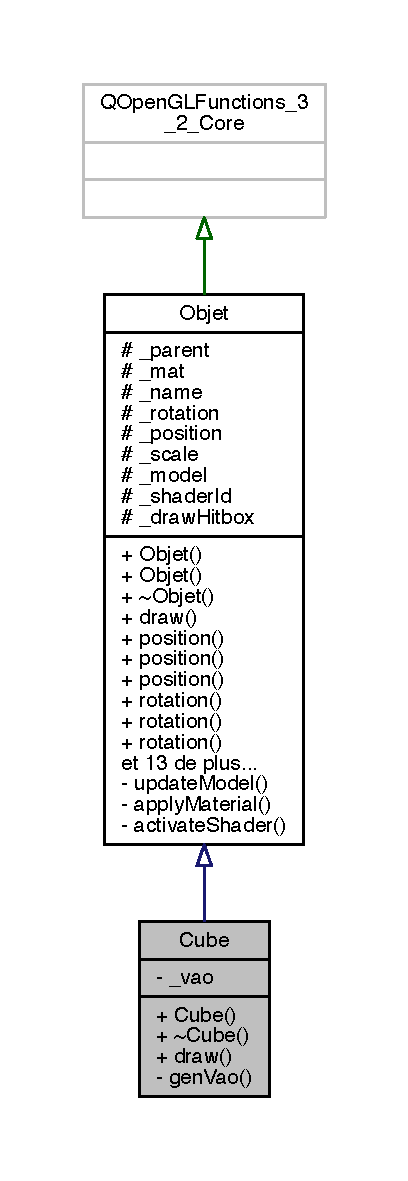
\includegraphics[height=550pt]{class_cube__inherit__graph}
\end{center}
\end{figure}


Graphe de collaboration de Cube\+:
\nopagebreak
\begin{figure}[H]
\begin{center}
\leavevmode
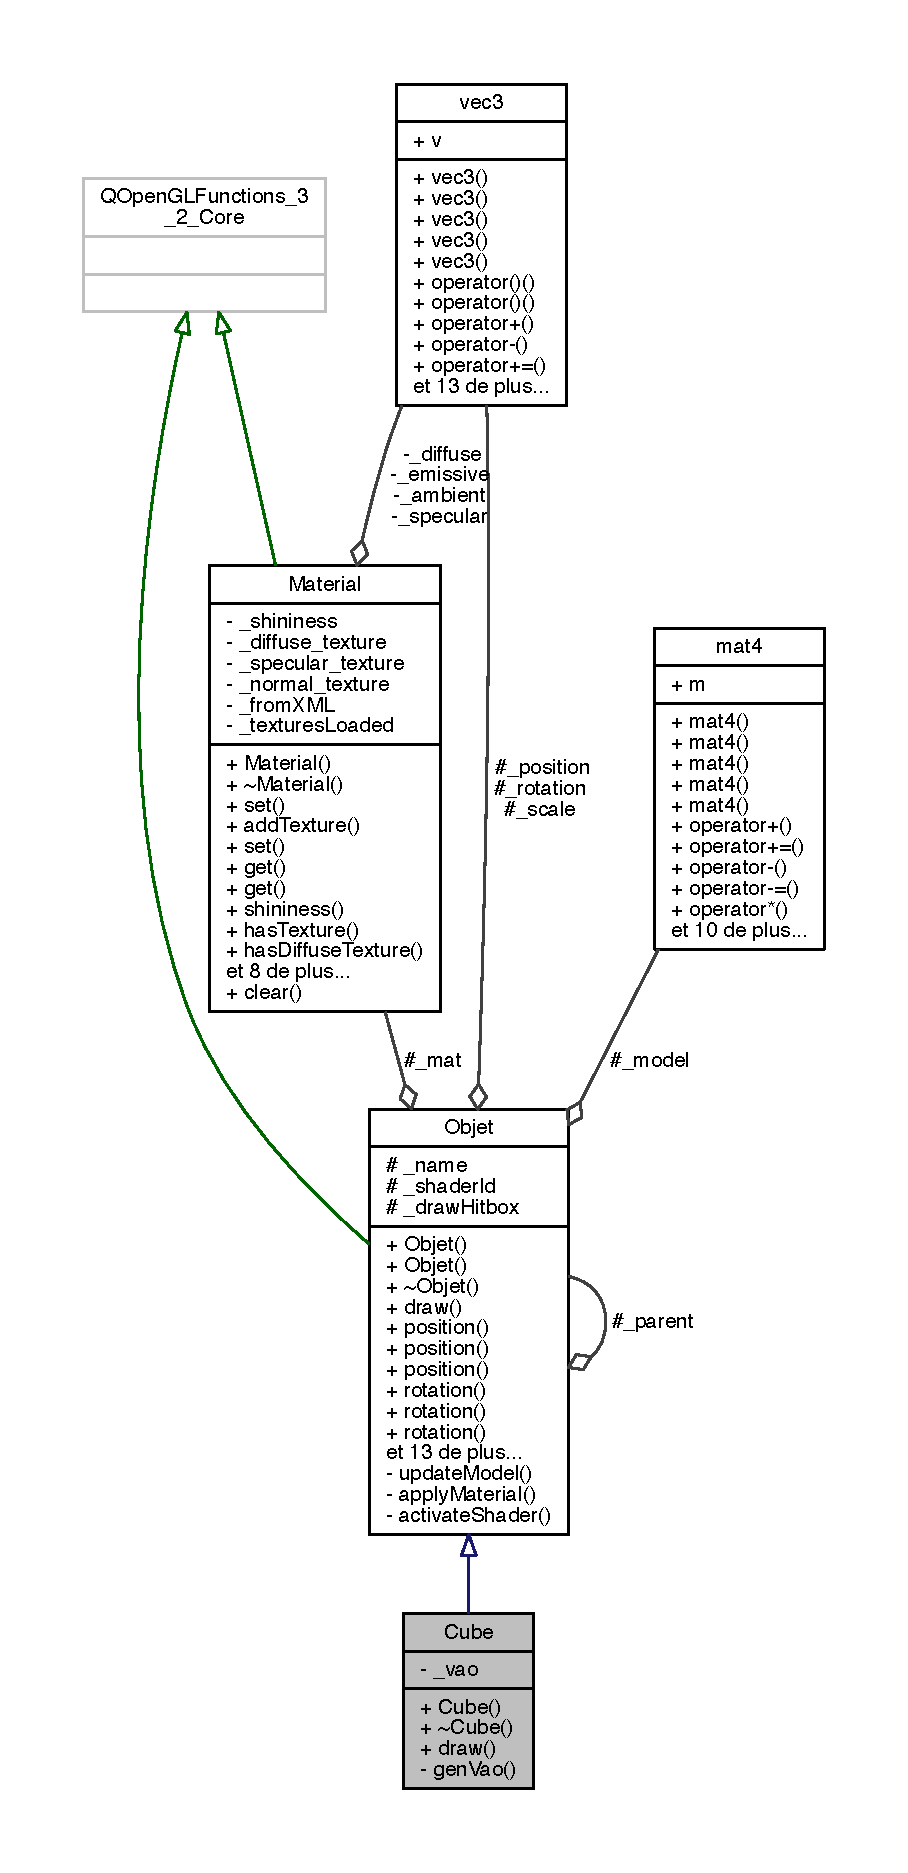
\includegraphics[height=550pt]{class_cube__coll__graph}
\end{center}
\end{figure}
\subsection*{Fonctions membres publiques}
\begin{DoxyCompactItemize}
\item 
\hyperlink{class_cube_a6d016e01f3fee45cff97be27ff7175d8}{Cube} (\hyperlink{class_material}{Material} $\ast$mat=N\+U\+L\+L, \hyperlink{structvec3}{vec3} \hyperlink{class_objet_ac69a1b459bcb4433099c8cfbff06b209}{rotation}=\hyperlink{structvec3}{vec3}(), \hyperlink{structvec3}{vec3} \hyperlink{class_objet_a0e109bc790b14328202dd2546b04e2fd}{position}=\hyperlink{structvec3}{vec3}())
\begin{DoxyCompactList}\small\item\em Constructeur du cube. \end{DoxyCompactList}\item 
\hyperlink{class_cube_aa814e979cecb8c451fdb332ded2cea1e}{$\sim$\+Cube} ()
\begin{DoxyCompactList}\small\item\em Destructeur du cube. \end{DoxyCompactList}\item 
void \hyperlink{class_cube_ab26b72a81376fd5dc4fcc7f0b715b087}{draw} ()
\begin{DoxyCompactList}\small\item\em Affiche le cube. \end{DoxyCompactList}\end{DoxyCompactItemize}
\subsection*{Fonctions membres privées}
\begin{DoxyCompactItemize}
\item 
void \hyperlink{class_cube_a06f4c8632c223f8d8c34971e55a2dafc}{gen\+Vao} ()
\begin{DoxyCompactList}\small\item\em Génère les vbo et le vao pour l'affichage du cube. \end{DoxyCompactList}\end{DoxyCompactItemize}
\subsection*{Attributs privés statiques}
\begin{DoxyCompactItemize}
\item 
static G\+Luint \hyperlink{class_cube_ae474ca8293842dd9ac83a8c606991eac}{\+\_\+vao} = 0
\end{DoxyCompactItemize}
\subsection*{Membres hérités additionnels}


\subsection{Description détaillée}
Primitive cube. 

\begin{DoxyWarning}{Avertissement}
Peut être plus utilisable 
\end{DoxyWarning}


\subsection{Documentation des constructeurs et destructeur}
\hypertarget{class_cube_a6d016e01f3fee45cff97be27ff7175d8}{\index{Cube@{Cube}!Cube@{Cube}}
\index{Cube@{Cube}!Cube@{Cube}}
\subsubsection[{Cube}]{\setlength{\rightskip}{0pt plus 5cm}Cube\+::\+Cube (
\begin{DoxyParamCaption}
\item[{{\bf Material} $\ast$}]{mat = {\ttfamily NULL}, }
\item[{{\bf vec3}}]{rotation = {\ttfamily {\bf vec3}()}, }
\item[{{\bf vec3}}]{position = {\ttfamily {\bf vec3}()}}
\end{DoxyParamCaption}
)}}\label{class_cube_a6d016e01f3fee45cff97be27ff7175d8}


Constructeur du cube. 

Génère le vao et les vbo s'ils n'ont pas déjà été générés 

Voici le graphe d'appel pour cette fonction \+:
\nopagebreak
\begin{figure}[H]
\begin{center}
\leavevmode
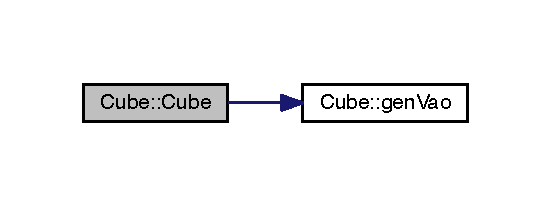
\includegraphics[width=265pt]{class_cube_a6d016e01f3fee45cff97be27ff7175d8_cgraph}
\end{center}
\end{figure}


\hypertarget{class_cube_aa814e979cecb8c451fdb332ded2cea1e}{\index{Cube@{Cube}!````~Cube@{$\sim$\+Cube}}
\index{````~Cube@{$\sim$\+Cube}!Cube@{Cube}}
\subsubsection[{$\sim$\+Cube}]{\setlength{\rightskip}{0pt plus 5cm}Cube\+::$\sim$\+Cube (
\begin{DoxyParamCaption}
{}
\end{DoxyParamCaption}
)}}\label{class_cube_aa814e979cecb8c451fdb332ded2cea1e}


Destructeur du cube. 



\subsection{Documentation des fonctions membres}
\hypertarget{class_cube_ab26b72a81376fd5dc4fcc7f0b715b087}{\index{Cube@{Cube}!draw@{draw}}
\index{draw@{draw}!Cube@{Cube}}
\subsubsection[{draw}]{\setlength{\rightskip}{0pt plus 5cm}void Cube\+::draw (
\begin{DoxyParamCaption}
{}
\end{DoxyParamCaption}
)\hspace{0.3cm}{\ttfamily [virtual]}}}\label{class_cube_ab26b72a81376fd5dc4fcc7f0b715b087}


Affiche le cube. 



Réimplémentée à partir de \hyperlink{class_objet_a5cc323f562964e00b947b2d908e206e7}{Objet}.



Voici le graphe d'appel pour cette fonction \+:
\nopagebreak
\begin{figure}[H]
\begin{center}
\leavevmode
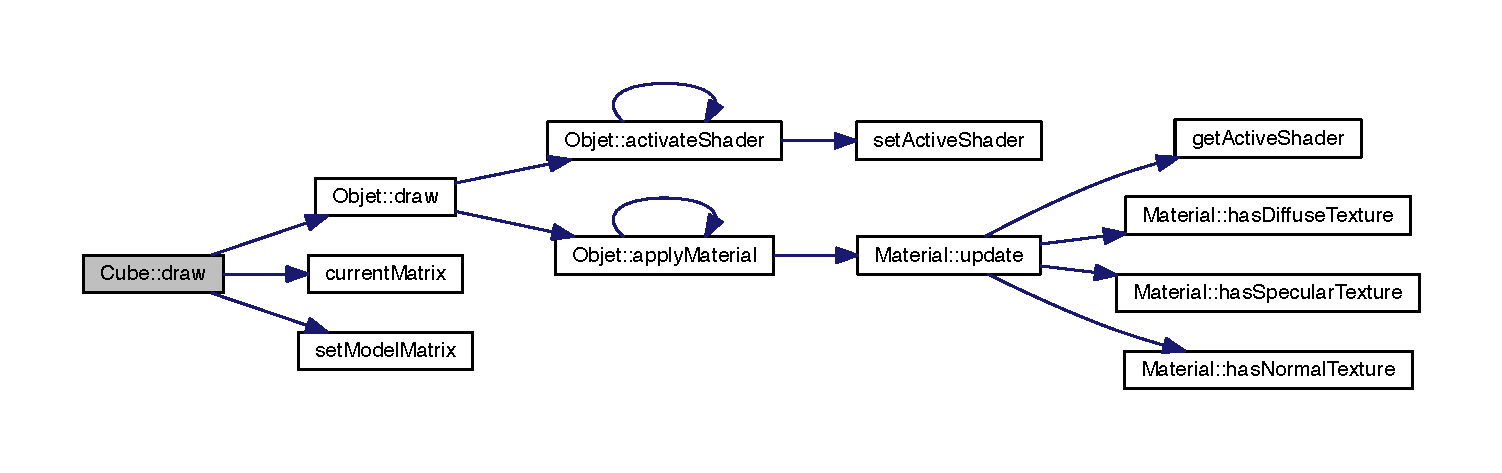
\includegraphics[width=350pt]{class_cube_ab26b72a81376fd5dc4fcc7f0b715b087_cgraph}
\end{center}
\end{figure}


\hypertarget{class_cube_a06f4c8632c223f8d8c34971e55a2dafc}{\index{Cube@{Cube}!gen\+Vao@{gen\+Vao}}
\index{gen\+Vao@{gen\+Vao}!Cube@{Cube}}
\subsubsection[{gen\+Vao}]{\setlength{\rightskip}{0pt plus 5cm}void Cube\+::gen\+Vao (
\begin{DoxyParamCaption}
{}
\end{DoxyParamCaption}
)\hspace{0.3cm}{\ttfamily [private]}}}\label{class_cube_a06f4c8632c223f8d8c34971e55a2dafc}


Génère les vbo et le vao pour l'affichage du cube. 



Voici le graphe des appelants de cette fonction \+:
\nopagebreak
\begin{figure}[H]
\begin{center}
\leavevmode
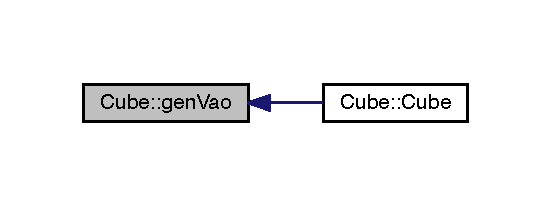
\includegraphics[width=265pt]{class_cube_a06f4c8632c223f8d8c34971e55a2dafc_icgraph}
\end{center}
\end{figure}




\subsection{Documentation des données membres}
\hypertarget{class_cube_ae474ca8293842dd9ac83a8c606991eac}{\index{Cube@{Cube}!\+\_\+vao@{\+\_\+vao}}
\index{\+\_\+vao@{\+\_\+vao}!Cube@{Cube}}
\subsubsection[{\+\_\+vao}]{\setlength{\rightskip}{0pt plus 5cm}G\+Luint Cube\+::\+\_\+vao = 0\hspace{0.3cm}{\ttfamily [static]}, {\ttfamily [private]}}}\label{class_cube_ae474ca8293842dd9ac83a8c606991eac}
$<$ Id du Vao du cube 

La documentation de cette classe a été générée à partir des fichiers suivants \+:\begin{DoxyCompactItemize}
\item 
objets/\hyperlink{cube_8hpp}{cube.\+hpp}\item 
objets/\hyperlink{cube_8cpp}{cube.\+cpp}\end{DoxyCompactItemize}

\hypertarget{class_donuts}{\section{Donuts Class Reference}
\label{class_donuts}\index{Donuts@{Donuts}}
}


Primitive tore.  




{\ttfamily \#include $<$donuts.\+hpp$>$}

Inheritance diagram for Donuts\+:\begin{figure}[H]
\begin{center}
\leavevmode
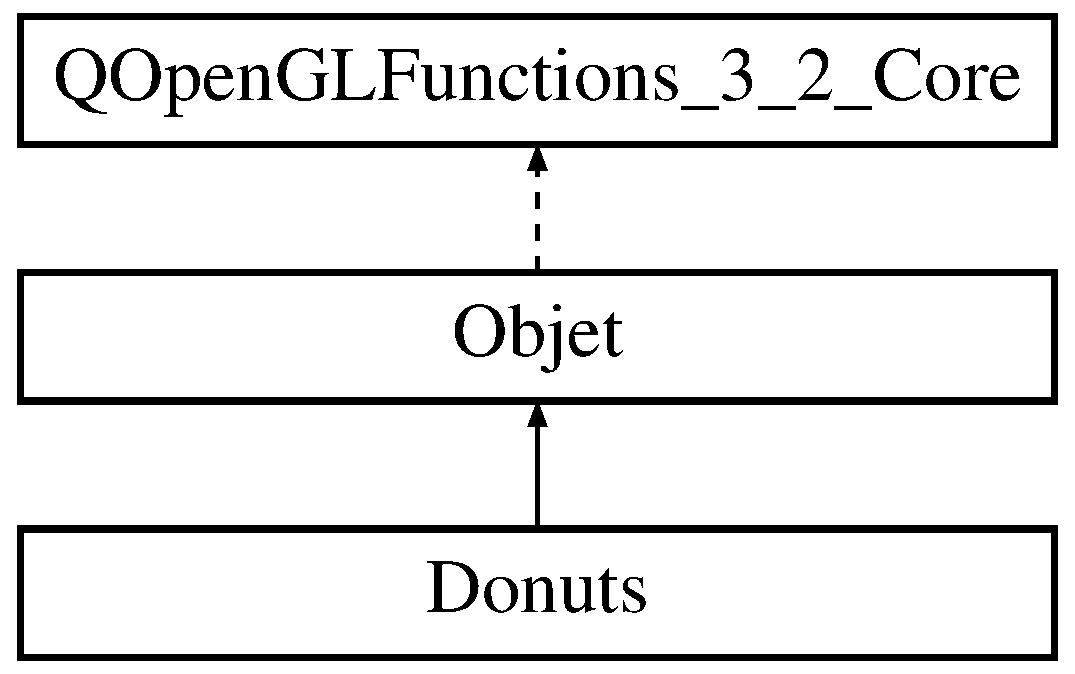
\includegraphics[height=3.000000cm]{class_donuts}
\end{center}
\end{figure}
\subsection*{Public Member Functions}
\begin{DoxyCompactItemize}
\item 
\hyperlink{class_donuts_a91d8d9b011ed1f7e406a2906f2b6e898}{Donuts} (G\+Ldouble \hyperlink{class_donuts_ae3db8d4ea17228ed43d388bac7fb35b3}{m\+\_\+radius}=1, G\+Ldouble \hyperlink{class_donuts_a5050c790a74b5313a06b818a7f3e8723}{m\+\_\+radius\+\_\+donuts}=1, G\+Lint \hyperlink{class_donuts_a2214ac47effb92c5de33fa7c57d28694}{m\+\_\+slices}=1, G\+Lint \hyperlink{class_donuts_a5273bc3a4bdada5e4302b35d49bdd550}{m\+\_\+stacks}=1, \hyperlink{class_material}{Material} $\ast$mat=N\+U\+L\+L, \hyperlink{structvec3}{vec3} \hyperlink{class_objet_ac69a1b459bcb4433099c8cfbff06b209}{rotation}=\hyperlink{structvec3}{vec3}(), \hyperlink{structvec3}{vec3} \hyperlink{class_objet_a0e109bc790b14328202dd2546b04e2fd}{position}=\hyperlink{structvec3}{vec3}())
\item 
\hyperlink{class_donuts_aea6536802eeb29b4fa4eee2f7e1ea626}{$\sim$\+Donuts} ()
\item 
void \hyperlink{class_donuts_a5a7932c8494905ba09bb515a01e6c91d}{draw} ()
\begin{DoxyCompactList}\small\item\em Affichage de l'\hyperlink{class_objet}{Objet}. \end{DoxyCompactList}\end{DoxyCompactItemize}
\subsection*{Private Member Functions}
\begin{DoxyCompactItemize}
\item 
void \hyperlink{class_donuts_aff7950429cf43ee2898c6f1a6545b174}{gen\+Vao} ()
\end{DoxyCompactItemize}
\subsection*{Private Attributes}
\begin{DoxyCompactItemize}
\item 
G\+Luint \hyperlink{class_donuts_a659c70b043ddc2ebcdc64bcb58c1e621}{\+\_\+vao}
\item 
G\+Ldouble \hyperlink{class_donuts_ae3db8d4ea17228ed43d388bac7fb35b3}{m\+\_\+radius}
\item 
G\+Ldouble \hyperlink{class_donuts_a5050c790a74b5313a06b818a7f3e8723}{m\+\_\+radius\+\_\+donuts}
\item 
G\+Lint \hyperlink{class_donuts_a2214ac47effb92c5de33fa7c57d28694}{m\+\_\+slices}
\item 
G\+Lint \hyperlink{class_donuts_a5273bc3a4bdada5e4302b35d49bdd550}{m\+\_\+stacks}
\item 
G\+Lsizei \hyperlink{class_donuts_aac0118d276a512d287a9bc1f4c7d249d}{nbvertex}
\end{DoxyCompactItemize}
\subsection*{Additional Inherited Members}


\subsection{Detailed Description}
Primitive tore. 

\begin{DoxyWarning}{Warning}
Peut être plus utilisable 
\end{DoxyWarning}
\begin{DoxySeeAlso}{See also}
\hyperlink{class_cube}{Cube} 
\end{DoxySeeAlso}


\subsection{Constructor \& Destructor Documentation}
\hypertarget{class_donuts_a91d8d9b011ed1f7e406a2906f2b6e898}{\index{Donuts@{Donuts}!Donuts@{Donuts}}
\index{Donuts@{Donuts}!Donuts@{Donuts}}
\subsubsection[{Donuts}]{\setlength{\rightskip}{0pt plus 5cm}Donuts\+::\+Donuts (
\begin{DoxyParamCaption}
\item[{G\+Ldouble}]{m\+\_\+radius = {\ttfamily 1}, }
\item[{G\+Ldouble}]{m\+\_\+radius\+\_\+donuts = {\ttfamily 1}, }
\item[{G\+Lint}]{m\+\_\+slices = {\ttfamily 1}, }
\item[{G\+Lint}]{m\+\_\+stacks = {\ttfamily 1}, }
\item[{{\bf Material} $\ast$}]{mat = {\ttfamily NULL}, }
\item[{{\bf vec3}}]{rotation = {\ttfamily {\bf vec3}()}, }
\item[{{\bf vec3}}]{position = {\ttfamily {\bf vec3}()}}
\end{DoxyParamCaption}
)}}\label{class_donuts_a91d8d9b011ed1f7e406a2906f2b6e898}
\hypertarget{class_donuts_aea6536802eeb29b4fa4eee2f7e1ea626}{\index{Donuts@{Donuts}!````~Donuts@{$\sim$\+Donuts}}
\index{````~Donuts@{$\sim$\+Donuts}!Donuts@{Donuts}}
\subsubsection[{$\sim$\+Donuts}]{\setlength{\rightskip}{0pt plus 5cm}Donuts\+::$\sim$\+Donuts (
\begin{DoxyParamCaption}
{}
\end{DoxyParamCaption}
)}}\label{class_donuts_aea6536802eeb29b4fa4eee2f7e1ea626}


\subsection{Member Function Documentation}
\hypertarget{class_donuts_a5a7932c8494905ba09bb515a01e6c91d}{\index{Donuts@{Donuts}!draw@{draw}}
\index{draw@{draw}!Donuts@{Donuts}}
\subsubsection[{draw}]{\setlength{\rightskip}{0pt plus 5cm}void Donuts\+::draw (
\begin{DoxyParamCaption}
{}
\end{DoxyParamCaption}
)\hspace{0.3cm}{\ttfamily [virtual]}}}\label{class_donuts_a5a7932c8494905ba09bb515a01e6c91d}


Affichage de l'\hyperlink{class_objet}{Objet}. 

Active le shader de l'\hyperlink{class_objet}{Objet} et applique le material 

Reimplemented from \hyperlink{class_objet_a5cc323f562964e00b947b2d908e206e7}{Objet}.

\hypertarget{class_donuts_aff7950429cf43ee2898c6f1a6545b174}{\index{Donuts@{Donuts}!gen\+Vao@{gen\+Vao}}
\index{gen\+Vao@{gen\+Vao}!Donuts@{Donuts}}
\subsubsection[{gen\+Vao}]{\setlength{\rightskip}{0pt plus 5cm}void Donuts\+::gen\+Vao (
\begin{DoxyParamCaption}
{}
\end{DoxyParamCaption}
)\hspace{0.3cm}{\ttfamily [private]}}}\label{class_donuts_aff7950429cf43ee2898c6f1a6545b174}


\subsection{Member Data Documentation}
\hypertarget{class_donuts_a659c70b043ddc2ebcdc64bcb58c1e621}{\index{Donuts@{Donuts}!\+\_\+vao@{\+\_\+vao}}
\index{\+\_\+vao@{\+\_\+vao}!Donuts@{Donuts}}
\subsubsection[{\+\_\+vao}]{\setlength{\rightskip}{0pt plus 5cm}G\+Luint Donuts\+::\+\_\+vao\hspace{0.3cm}{\ttfamily [private]}}}\label{class_donuts_a659c70b043ddc2ebcdc64bcb58c1e621}
\hypertarget{class_donuts_ae3db8d4ea17228ed43d388bac7fb35b3}{\index{Donuts@{Donuts}!m\+\_\+radius@{m\+\_\+radius}}
\index{m\+\_\+radius@{m\+\_\+radius}!Donuts@{Donuts}}
\subsubsection[{m\+\_\+radius}]{\setlength{\rightskip}{0pt plus 5cm}G\+Ldouble Donuts\+::m\+\_\+radius\hspace{0.3cm}{\ttfamily [private]}}}\label{class_donuts_ae3db8d4ea17228ed43d388bac7fb35b3}
\hypertarget{class_donuts_a5050c790a74b5313a06b818a7f3e8723}{\index{Donuts@{Donuts}!m\+\_\+radius\+\_\+donuts@{m\+\_\+radius\+\_\+donuts}}
\index{m\+\_\+radius\+\_\+donuts@{m\+\_\+radius\+\_\+donuts}!Donuts@{Donuts}}
\subsubsection[{m\+\_\+radius\+\_\+donuts}]{\setlength{\rightskip}{0pt plus 5cm}G\+Ldouble Donuts\+::m\+\_\+radius\+\_\+donuts\hspace{0.3cm}{\ttfamily [private]}}}\label{class_donuts_a5050c790a74b5313a06b818a7f3e8723}
\hypertarget{class_donuts_a2214ac47effb92c5de33fa7c57d28694}{\index{Donuts@{Donuts}!m\+\_\+slices@{m\+\_\+slices}}
\index{m\+\_\+slices@{m\+\_\+slices}!Donuts@{Donuts}}
\subsubsection[{m\+\_\+slices}]{\setlength{\rightskip}{0pt plus 5cm}G\+Lint Donuts\+::m\+\_\+slices\hspace{0.3cm}{\ttfamily [private]}}}\label{class_donuts_a2214ac47effb92c5de33fa7c57d28694}
\hypertarget{class_donuts_a5273bc3a4bdada5e4302b35d49bdd550}{\index{Donuts@{Donuts}!m\+\_\+stacks@{m\+\_\+stacks}}
\index{m\+\_\+stacks@{m\+\_\+stacks}!Donuts@{Donuts}}
\subsubsection[{m\+\_\+stacks}]{\setlength{\rightskip}{0pt plus 5cm}G\+Lint Donuts\+::m\+\_\+stacks\hspace{0.3cm}{\ttfamily [private]}}}\label{class_donuts_a5273bc3a4bdada5e4302b35d49bdd550}
\hypertarget{class_donuts_aac0118d276a512d287a9bc1f4c7d249d}{\index{Donuts@{Donuts}!nbvertex@{nbvertex}}
\index{nbvertex@{nbvertex}!Donuts@{Donuts}}
\subsubsection[{nbvertex}]{\setlength{\rightskip}{0pt plus 5cm}G\+Lsizei Donuts\+::nbvertex\hspace{0.3cm}{\ttfamily [private]}}}\label{class_donuts_aac0118d276a512d287a9bc1f4c7d249d}


The documentation for this class was generated from the following files\+:\begin{DoxyCompactItemize}
\item 
objets/\hyperlink{donuts_8hpp}{donuts.\+hpp}\item 
objets/\hyperlink{donuts_8cpp}{donuts.\+cpp}\end{DoxyCompactItemize}

\hypertarget{class_light}{\section{Light Class Reference}
\label{class_light}\index{Light@{Light}}
}


Lumière pour la \hyperlink{class_scene}{Scene}.  




{\ttfamily \#include $<$light.\+hpp$>$}

Inheritance diagram for Light\+:\begin{figure}[H]
\begin{center}
\leavevmode
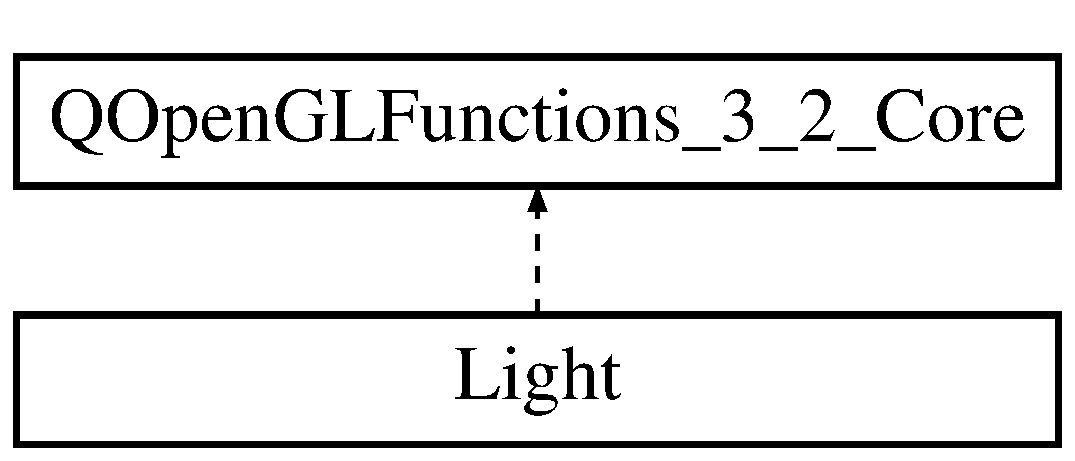
\includegraphics[height=2.000000cm]{class_light}
\end{center}
\end{figure}
\subsection*{Public Member Functions}
\begin{DoxyCompactItemize}
\item 
\hyperlink{class_light_aa7bcc37dee068f7266f86e07a3dfe4f0}{Light} (\hyperlink{structvec3}{vec3} position=\hyperlink{structvec3}{vec3}(0.\+0, 0.\+0, 0.\+0), \hyperlink{structvec3}{vec3} diffuse=\hyperlink{structvec3}{vec3}(0.\+8, 0.\+8, 0.\+8), \hyperlink{structvec3}{vec3} specular=\hyperlink{structvec3}{vec3}(0.\+8, 0.\+8, 0.\+8))
\begin{DoxyCompactList}\small\item\em Constructeur d'une lumière. \end{DoxyCompactList}\item 
\hyperlink{class_light_ad0e59fad13bb6cfadc25b2c477e9ddc7}{$\sim$\+Light} ()
\begin{DoxyCompactList}\small\item\em Destructeur. \end{DoxyCompactList}\item 
void \hyperlink{class_light_a9fcc4b3ffdeedbe214ee8384c7d311b9}{set} (G\+Lenum type, \hyperlink{structvec3}{vec3} value)
\begin{DoxyCompactList}\small\item\em Met à jour une composante de la lumière. \end{DoxyCompactList}\item 
\hyperlink{structvec3}{vec3} \hyperlink{class_light_ad0f5f939bc047e39c6deb2e264a5a2c1}{get} (G\+Lenum type) const 
\begin{DoxyCompactList}\small\item\em Récupère la valeur d'une composante de la lumière. \end{DoxyCompactList}\item 
\hyperlink{structvec3}{vec3} \& \hyperlink{class_light_a74a0381255c1c7e002ac583401a46de0}{get} (G\+Lenum type)
\begin{DoxyCompactList}\small\item\em Récupère la valeur d'une composante de la lumière. \end{DoxyCompactList}\item 
void \hyperlink{class_light_ade4c742c8ca2c014d74c659fa615ffd7}{update} (unsigned char number)
\begin{DoxyCompactList}\small\item\em Met à jour le shader avec les infos de la lumière. \end{DoxyCompactList}\end{DoxyCompactItemize}
\subsection*{Static Public Member Functions}
\begin{DoxyCompactItemize}
\item 
static void \hyperlink{class_light_a33a43afc95ed75a8970f523cb3f800fa}{disable} (unsigned char number)
\begin{DoxyCompactList}\small\item\em Désactive la lumière dans le shader. \end{DoxyCompactList}\item 
static void \hyperlink{class_light_a53ce58fd783207da18aa7dc3465841ac}{update\+Ambient} ()
\begin{DoxyCompactList}\small\item\em Met à jour la lumière ambient. \end{DoxyCompactList}\item 
static void \hyperlink{class_light_a1eae781d5e7a95c9dcc9bd76838496df}{ambient} (const \hyperlink{structvec3}{vec3} \&v)
\begin{DoxyCompactList}\small\item\em Modifie la composante ambient de la lumière. \end{DoxyCompactList}\item 
static \hyperlink{structvec3}{vec3} \& \hyperlink{class_light_a4f9a64ec04c9854d02a67cd2ceb6760c}{ambient} ()
\begin{DoxyCompactList}\small\item\em retourne le vecteur des composantes ambient \end{DoxyCompactList}\end{DoxyCompactItemize}
\subsection*{Private Attributes}
\begin{DoxyCompactItemize}
\item 
\hyperlink{structvec3}{vec3} \hyperlink{class_light_a3af8c823a869606782bd9e1872586b72}{\+\_\+position}
\item 
\hyperlink{structvec3}{vec3} \hyperlink{class_light_a32445f2054766ef532c29eb514b2599d}{\+\_\+diffuse}
\item 
\hyperlink{structvec3}{vec3} \hyperlink{class_light_a36414dc1e8a75b36652bc5a12b2ea43d}{\+\_\+specular}
\end{DoxyCompactItemize}
\subsection*{Static Private Attributes}
\begin{DoxyCompactItemize}
\item 
static \hyperlink{structvec3}{vec3} \hyperlink{class_light_ab139b739498b75944c99203027332ad9}{\+\_\+ambient}
\end{DoxyCompactItemize}


\subsection{Detailed Description}
Lumière pour la \hyperlink{class_scene}{Scene}. 

Gère une lumière pour la scène

\begin{DoxyWarning}{Warning}
seul les lumières positionnelles sont gérées pour l'instant 
\end{DoxyWarning}
\begin{DoxyRefDesc}{Todo}
\item[\hyperlink{todo__todo000001}{Todo}]attenuation de la lumière par lumière et plus globale \end{DoxyRefDesc}


\subsection{Constructor \& Destructor Documentation}
\hypertarget{class_light_aa7bcc37dee068f7266f86e07a3dfe4f0}{\index{Light@{Light}!Light@{Light}}
\index{Light@{Light}!Light@{Light}}
\subsubsection[{Light}]{\setlength{\rightskip}{0pt plus 5cm}Light\+::\+Light (
\begin{DoxyParamCaption}
\item[{{\bf vec3}}]{position = {\ttfamily {\bf vec3}(0.0,~0.0,~0.0)}, }
\item[{{\bf vec3}}]{diffuse = {\ttfamily {\bf vec3}(0.8,~0.8,~0.8)}, }
\item[{{\bf vec3}}]{specular = {\ttfamily {\bf vec3}(0.8,~0.8,~0.8)}}
\end{DoxyParamCaption}
)}}\label{class_light_aa7bcc37dee068f7266f86e07a3dfe4f0}


Constructeur d'une lumière. 


\begin{DoxyParams}{Parameters}
{\em position} & position de la lumière \\
\hline
{\em diffuse} & composante diffuse de la lumière \\
\hline
{\em specular} & composante spéculaire de la lumière \\
\hline
{\em number} & correspond au slot de la lumière qui sera utilisé dans le shader\\
\hline
\end{DoxyParams}
\begin{DoxyWarning}{Warning}
number doit appartenir à \mbox{[}0,7\mbox{]} 
\end{DoxyWarning}
\hypertarget{class_light_ad0e59fad13bb6cfadc25b2c477e9ddc7}{\index{Light@{Light}!````~Light@{$\sim$\+Light}}
\index{````~Light@{$\sim$\+Light}!Light@{Light}}
\subsubsection[{$\sim$\+Light}]{\setlength{\rightskip}{0pt plus 5cm}Light\+::$\sim$\+Light (
\begin{DoxyParamCaption}
{}
\end{DoxyParamCaption}
)}}\label{class_light_ad0e59fad13bb6cfadc25b2c477e9ddc7}


Destructeur. 

\begin{DoxyRefDesc}{Todo}
\item[\hyperlink{todo__todo000002}{Todo}]Vérifier que la lumière est désactivée dans tout les shader \end{DoxyRefDesc}


\subsection{Member Function Documentation}
\hypertarget{class_light_a1eae781d5e7a95c9dcc9bd76838496df}{\index{Light@{Light}!ambient@{ambient}}
\index{ambient@{ambient}!Light@{Light}}
\subsubsection[{ambient}]{\setlength{\rightskip}{0pt plus 5cm}static void Light\+::ambient (
\begin{DoxyParamCaption}
\item[{const {\bf vec3} \&}]{v}
\end{DoxyParamCaption}
)\hspace{0.3cm}{\ttfamily [inline]}, {\ttfamily [static]}}}\label{class_light_a1eae781d5e7a95c9dcc9bd76838496df}


Modifie la composante ambient de la lumière. 


\begin{DoxyParams}{Parameters}
{\em v} & nouvelle composante \\
\hline
\end{DoxyParams}
\hypertarget{class_light_a4f9a64ec04c9854d02a67cd2ceb6760c}{\index{Light@{Light}!ambient@{ambient}}
\index{ambient@{ambient}!Light@{Light}}
\subsubsection[{ambient}]{\setlength{\rightskip}{0pt plus 5cm}static {\bf vec3}\& Light\+::ambient (
\begin{DoxyParamCaption}
{}
\end{DoxyParamCaption}
)\hspace{0.3cm}{\ttfamily [inline]}, {\ttfamily [static]}}}\label{class_light_a4f9a64ec04c9854d02a67cd2ceb6760c}


retourne le vecteur des composantes ambient 

\hypertarget{class_light_a33a43afc95ed75a8970f523cb3f800fa}{\index{Light@{Light}!disable@{disable}}
\index{disable@{disable}!Light@{Light}}
\subsubsection[{disable}]{\setlength{\rightskip}{0pt plus 5cm}void Light\+::disable (
\begin{DoxyParamCaption}
\item[{unsigned char}]{number}
\end{DoxyParamCaption}
)\hspace{0.3cm}{\ttfamily [static]}}}\label{class_light_a33a43afc95ed75a8970f523cb3f800fa}


Désactive la lumière dans le shader. 


\begin{DoxyParams}{Parameters}
{\em number} & numéro de la lumière à désactiver \\
\hline
\end{DoxyParams}
\hypertarget{class_light_ad0f5f939bc047e39c6deb2e264a5a2c1}{\index{Light@{Light}!get@{get}}
\index{get@{get}!Light@{Light}}
\subsubsection[{get}]{\setlength{\rightskip}{0pt plus 5cm}{\bf vec3} Light\+::get (
\begin{DoxyParamCaption}
\item[{G\+Lenum}]{type}
\end{DoxyParamCaption}
) const}}\label{class_light_ad0f5f939bc047e39c6deb2e264a5a2c1}


Récupère la valeur d'une composante de la lumière. 


\begin{DoxyParams}{Parameters}
{\em type} & composante voulu, doit être parmis (G\+L\+\_\+\+P\+O\+S\+I\+T\+I\+O\+N, G\+L\+\_\+\+A\+M\+B\+I\+E\+N\+T, G\+L\+\_\+\+D\+I\+F\+F\+U\+S\+E, G\+L\+\_\+\+S\+P\+E\+C\+U\+L\+A\+R) \\
\hline
\end{DoxyParams}
\begin{DoxyReturn}{Returns}
valeur 
\end{DoxyReturn}
\hypertarget{class_light_a74a0381255c1c7e002ac583401a46de0}{\index{Light@{Light}!get@{get}}
\index{get@{get}!Light@{Light}}
\subsubsection[{get}]{\setlength{\rightskip}{0pt plus 5cm}{\bf vec3} \& Light\+::get (
\begin{DoxyParamCaption}
\item[{G\+Lenum}]{type}
\end{DoxyParamCaption}
)}}\label{class_light_a74a0381255c1c7e002ac583401a46de0}


Récupère la valeur d'une composante de la lumière. 


\begin{DoxyParams}{Parameters}
{\em type} & composante voulu, doit être parmis (G\+L\+\_\+\+P\+O\+S\+I\+T\+I\+O\+N, G\+L\+\_\+\+A\+M\+B\+I\+E\+N\+T, G\+L\+\_\+\+D\+I\+F\+F\+U\+S\+E, G\+L\+\_\+\+S\+P\+E\+C\+U\+L\+A\+R) \\
\hline
\end{DoxyParams}
\begin{DoxyReturn}{Returns}
valeur 
\end{DoxyReturn}
\begin{DoxyWarning}{Warning}
si le type n'est pas dans les 4 gérés résultat imprévisible 
\end{DoxyWarning}
\hypertarget{class_light_a9fcc4b3ffdeedbe214ee8384c7d311b9}{\index{Light@{Light}!set@{set}}
\index{set@{set}!Light@{Light}}
\subsubsection[{set}]{\setlength{\rightskip}{0pt plus 5cm}void Light\+::set (
\begin{DoxyParamCaption}
\item[{G\+Lenum}]{type, }
\item[{{\bf vec3}}]{value}
\end{DoxyParamCaption}
)}}\label{class_light_a9fcc4b3ffdeedbe214ee8384c7d311b9}


Met à jour une composante de la lumière. 


\begin{DoxyParams}{Parameters}
{\em type} & composante à modifier, doit être parmis (G\+L\+\_\+\+P\+O\+S\+I\+T\+I\+O\+N, G\+L\+\_\+\+A\+M\+B\+I\+E\+N\+T, G\+L\+\_\+\+D\+I\+F\+F\+U\+S\+E, G\+L\+\_\+\+S\+P\+E\+C\+U\+L\+A\+R) \\
\hline
{\em value} & valeur \\
\hline
\end{DoxyParams}
\hypertarget{class_light_ade4c742c8ca2c014d74c659fa615ffd7}{\index{Light@{Light}!update@{update}}
\index{update@{update}!Light@{Light}}
\subsubsection[{update}]{\setlength{\rightskip}{0pt plus 5cm}void Light\+::update (
\begin{DoxyParamCaption}
\item[{unsigned char}]{number}
\end{DoxyParamCaption}
)}}\label{class_light_ade4c742c8ca2c014d74c659fa615ffd7}


Met à jour le shader avec les infos de la lumière. 


\begin{DoxyParams}{Parameters}
{\em number} & slot de lumière à utiliser dans la shader \\
\hline
\end{DoxyParams}
\hypertarget{class_light_a53ce58fd783207da18aa7dc3465841ac}{\index{Light@{Light}!update\+Ambient@{update\+Ambient}}
\index{update\+Ambient@{update\+Ambient}!Light@{Light}}
\subsubsection[{update\+Ambient}]{\setlength{\rightskip}{0pt plus 5cm}void Light\+::update\+Ambient (
\begin{DoxyParamCaption}
{}
\end{DoxyParamCaption}
)\hspace{0.3cm}{\ttfamily [static]}}}\label{class_light_a53ce58fd783207da18aa7dc3465841ac}


Met à jour la lumière ambient. 



\subsection{Member Data Documentation}
\hypertarget{class_light_ab139b739498b75944c99203027332ad9}{\index{Light@{Light}!\+\_\+ambient@{\+\_\+ambient}}
\index{\+\_\+ambient@{\+\_\+ambient}!Light@{Light}}
\subsubsection[{\+\_\+ambient}]{\setlength{\rightskip}{0pt plus 5cm}{\bf vec3} Light\+::\+\_\+ambient\hspace{0.3cm}{\ttfamily [static]}, {\ttfamily [private]}}}\label{class_light_ab139b739498b75944c99203027332ad9}
La composante ambient est commune à toutes les lumières \hypertarget{class_light_a32445f2054766ef532c29eb514b2599d}{\index{Light@{Light}!\+\_\+diffuse@{\+\_\+diffuse}}
\index{\+\_\+diffuse@{\+\_\+diffuse}!Light@{Light}}
\subsubsection[{\+\_\+diffuse}]{\setlength{\rightskip}{0pt plus 5cm}{\bf vec3} Light\+::\+\_\+diffuse\hspace{0.3cm}{\ttfamily [private]}}}\label{class_light_a32445f2054766ef532c29eb514b2599d}
\hypertarget{class_light_a3af8c823a869606782bd9e1872586b72}{\index{Light@{Light}!\+\_\+position@{\+\_\+position}}
\index{\+\_\+position@{\+\_\+position}!Light@{Light}}
\subsubsection[{\+\_\+position}]{\setlength{\rightskip}{0pt plus 5cm}{\bf vec3} Light\+::\+\_\+position\hspace{0.3cm}{\ttfamily [private]}}}\label{class_light_a3af8c823a869606782bd9e1872586b72}
\hypertarget{class_light_a36414dc1e8a75b36652bc5a12b2ea43d}{\index{Light@{Light}!\+\_\+specular@{\+\_\+specular}}
\index{\+\_\+specular@{\+\_\+specular}!Light@{Light}}
\subsubsection[{\+\_\+specular}]{\setlength{\rightskip}{0pt plus 5cm}{\bf vec3} Light\+::\+\_\+specular\hspace{0.3cm}{\ttfamily [private]}}}\label{class_light_a36414dc1e8a75b36652bc5a12b2ea43d}


The documentation for this class was generated from the following files\+:\begin{DoxyCompactItemize}
\item 
scene/\hyperlink{light_8hpp}{light.\+hpp}\item 
scene/\hyperlink{light_8cpp}{light.\+cpp}\end{DoxyCompactItemize}

\hypertarget{class_main_window}{\section{Main\+Window Class Reference}
\label{class_main_window}\index{Main\+Window@{Main\+Window}}
}


{\ttfamily \#include $<$mainwindows.\+hpp$>$}

Inheritance diagram for Main\+Window\+:\begin{figure}[H]
\begin{center}
\leavevmode
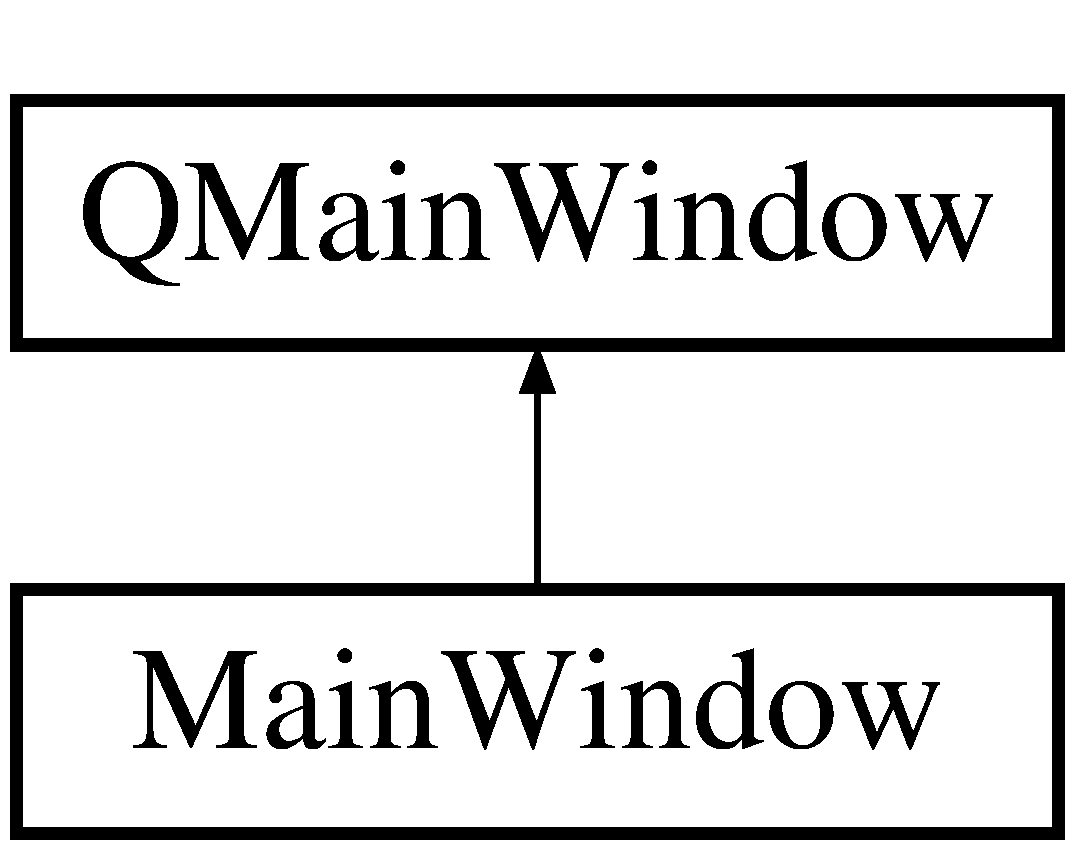
\includegraphics[height=2.000000cm]{class_main_window}
\end{center}
\end{figure}
\subsection*{Public Member Functions}
\begin{DoxyCompactItemize}
\item 
\hyperlink{class_main_window_a34c4b4207b46d11a4100c9b19f0e81bb}{Main\+Window} ()
\item 
\hyperlink{class_main_window_ae98d00a93bc118200eeef9f9bba1dba7}{$\sim$\+Main\+Window} ()
\end{DoxyCompactItemize}
\subsection*{Private Slots}
\begin{DoxyCompactItemize}
\item 
void \hyperlink{class_main_window_a6f837f331c40d27e47fbb0d6a73b040e}{Nouveau} ()
\item 
void \hyperlink{class_main_window_adbc60f34a13a49cc015dc4a124a588a1}{Ouvrir} ()
\item 
void \hyperlink{class_main_window_a8c07d91b87178ac0a1b88aabc45c6ddb}{Enregistrer} ()
\item 
void \hyperlink{class_main_window_a4558a3ff95a78f4a0e0d0adf312a6b8c}{Kiter} ()
\item 
void \hyperlink{class_main_window_a5277087cb1c0b01722b7a4ff436070ba}{Annuler} ()
\item 
void \hyperlink{class_main_window_ab2ff5da91852950471811fa93028dc0c}{Retablir} ()
\item 
void \hyperlink{class_main_window_a019328eaf07af3c9b8850e3db14fdf30}{Apercut} ()
\item 
void \hyperlink{class_main_window_a0b391dfd82e868b6f8badbc9717d6f49}{Culface} ()
\item 
void \hyperlink{class_main_window_a9a4d5849cf40a3ce50941e56cfa0be35}{Grille} ()
\item 
void \hyperlink{class_main_window_af26018b1d699cbf0a3f62048472cc489}{Importation3\+D} ()
\item 
void \hyperlink{class_main_window_a42d29fe9a2657a5c5563b3f1235a28e4}{ajoutlumiere} ()
\item 
void \hyperlink{class_main_window_a56f65a459f0caca9f71251663b200431}{validajoutlumiere} ()
\item 
void \hyperlink{class_main_window_a3a599353265f9c01a8780529aa5fed75}{ajoutmaterial} ()
\item 
void \hyperlink{class_main_window_a2d8cee622b78ccdeed758c51b9fb5b0e}{validajoutmaterial} ()
\item 
void \hyperlink{class_main_window_abd2acb261445354d2fd680c9b48bad77}{Racourcit} ()
\end{DoxyCompactItemize}
\subsection*{Private Member Functions}
\begin{DoxyCompactItemize}
\item 
void \hyperlink{class_main_window_a62cd8712fb41a754298f6f60eead2cb0}{create\+Actions} ()
\item 
void \hyperlink{class_main_window_aa4907b0251d305659e403c62921ef331}{create\+Menus} ()
\item 
void \hyperlink{class_main_window_a7b7fd06b9e7bfc83904b1d5b6503e9e9}{create\+Liste\+Dockwidget} ()
\item 
void \hyperlink{class_main_window_aeb57235ebc08860e680132db167c09b4}{create\+Tool\+Bar} ()
\end{DoxyCompactItemize}
\subsection*{Private Attributes}
\begin{DoxyCompactItemize}
\item 
Q\+Menu $\ast$ \hyperlink{class_main_window_ac5ad5607ac4e015f5b594aa73ca6703a}{Fichier}
\item 
Q\+Menu $\ast$ \hyperlink{class_main_window_af32c5a214657e6a6dd30269f81c8b450}{Edition}
\item 
Q\+Menu $\ast$ \hyperlink{class_main_window_a77f24d5ff1220ea72f7730d20672911c}{Affichage}
\item 
Q\+Menu $\ast$ \hyperlink{class_main_window_a8763d8624da754aef58d119d70462e60}{Outil}
\item 
Q\+Menu $\ast$ \hyperlink{class_main_window_ab9d17ad44a1ac962e46ac4af1a5732a0}{Aide}
\item 
Q\+Action $\ast$ \hyperlink{class_main_window_a193a37a0da1d22c48c64af3f6c5a6c51}{nouveau\+Act}
\item 
Q\+Action $\ast$ \hyperlink{class_main_window_ac02355cedb6a7337d9ee55d91dd9a4c0}{ouvrir\+Act}
\item 
Q\+Action $\ast$ \hyperlink{class_main_window_aaf23ba5444a4264c5c53fec9b729b2ba}{enregistrer\+Act}
\item 
Q\+Action $\ast$ \hyperlink{class_main_window_ac1517849e119e00fbbebe90570eabade}{kiter\+Act}
\item 
Q\+Action $\ast$ \hyperlink{class_main_window_ace04c15ff28b4931c15f823d0d2ed23b}{annuler\+Act}
\item 
Q\+Action $\ast$ \hyperlink{class_main_window_ab36e19495a8fe7e099772ea3ba4669c1}{retablir\+Act}
\item 
Q\+Action $\ast$ \hyperlink{class_main_window_a26d7fbeaa5d928206325ccccc9ed82c9}{apercut\+Act}
\item 
Q\+Action $\ast$ \hyperlink{class_main_window_acc241f6a81ac7e252fac333e8e725da3}{culface\+Act}
\item 
Q\+Action $\ast$ \hyperlink{class_main_window_a28c1cca30ba2fe676455f847c6f4a60a}{grille\+Act}
\item 
Q\+Action $\ast$ \hyperlink{class_main_window_a5c1ee7709fa8c1f29d7df9ee04b74ab8}{importation3\+D\+Act}
\item 
Q\+Menu $\ast$ \hyperlink{class_main_window_a6c2ded3bdffc863604d7890c554578d5}{ajoutelement}
\item 
Q\+Action $\ast$ \hyperlink{class_main_window_a04b22ecfd14e02f1dd5a5dd77b509f8e}{ajoutlumier\+Act}
\item 
Q\+Action $\ast$ \hyperlink{class_main_window_ae531eca2b9941c7f260f466edd97790e}{ajoutmaterial\+Act}
\item 
Q\+Dock\+Widget $\ast$ \hyperlink{class_main_window_a391dd00592f215079a80db989f24266e}{dockajoutlumiere}
\item 
Q\+Widget $\ast$ \hyperlink{class_main_window_a9e2c8a96b09dbbfaa041531420603b9e}{widgetajoutlumiere}
\item 
Q\+Push\+Button $\ast$ \hyperlink{class_main_window_a4f7a42439a3d1dbc5213e5d2282f5ab0}{boutonajoutlumiere}
\item 
Q\+Line\+Edit $\ast$ \hyperlink{class_main_window_a88ef14a32e7bd0694d8c970b700588c8}{lineeditnomajoutlumiere}
\item 
Q\+Label $\ast$ \hyperlink{class_main_window_ad38c142eee23820d2d4c87217ea3558a}{nomajoutlumiere}
\item 
Q\+Double\+Spin\+Box $\ast$ \hyperlink{class_main_window_a5286af2240735027e43e96856889ba2d}{spinpositionajoutlumierex}
\item 
Q\+Double\+Spin\+Box $\ast$ \hyperlink{class_main_window_af8f989d61672591976f45a3857bd4088}{spinpositionajoutlumierey}
\item 
Q\+Double\+Spin\+Box $\ast$ \hyperlink{class_main_window_a190e482131a28865d5cb0956a1149272}{spinpositionajoutlumierez}
\item 
Q\+Label $\ast$ \hyperlink{class_main_window_a3c50fe103c1d0f1278737bced7e2e452}{positionajoutlumiere}
\item 
Q\+Double\+Spin\+Box $\ast$ \hyperlink{class_main_window_a0c740f449736ce6c303b0675f954f050}{spindifajoutlumierex}
\item 
Q\+Double\+Spin\+Box $\ast$ \hyperlink{class_main_window_ae03c85b751d4a28e2916e66d82d7e72d}{spindifajoutlumierey}
\item 
Q\+Double\+Spin\+Box $\ast$ \hyperlink{class_main_window_afca1245690133c96c9e182b0b56c6006}{spindifajoutlumierez}
\item 
Q\+Label $\ast$ \hyperlink{class_main_window_a87d3bd68a5f4e2323110804c4111dcc9}{difajoutlumiere}
\item 
Q\+Double\+Spin\+Box $\ast$ \hyperlink{class_main_window_a433afe9bb63e53ccf2253eb39ee6ebd1}{spinspeajoutlumierex}
\item 
Q\+Double\+Spin\+Box $\ast$ \hyperlink{class_main_window_afd72a5b29130fa092fdb6cb9b05f937c}{spinspeajoutlumierey}
\item 
Q\+Double\+Spin\+Box $\ast$ \hyperlink{class_main_window_a69368f55e2df16fac69b4bc9b7b24696}{spinspeajoutlumierez}
\item 
Q\+Label $\ast$ \hyperlink{class_main_window_a549c42dd7554a4414ca34fc253457889}{speajoutlumiere}
\item 
Q\+H\+Box\+Layout $\ast$ \hyperlink{class_main_window_a0cffcdf1b642b23f05b7ed78beaeb066}{layoutnomajoutlumiere}
\item 
Q\+H\+Box\+Layout $\ast$ \hyperlink{class_main_window_a0afe930901084cdb5835537298d77219}{layoutposajoutlumiere}
\item 
Q\+H\+Box\+Layout $\ast$ \hyperlink{class_main_window_a8ce502c6bd1f174f2e13d491f0797056}{layoutdifajoutlumiere}
\item 
Q\+H\+Box\+Layout $\ast$ \hyperlink{class_main_window_a31b82741cd4c48d8e3b85981173fd1ad}{layoutspeajoutlumiere}
\item 
Q\+V\+Box\+Layout $\ast$ \hyperlink{class_main_window_ab54462c9ca68986b780c8fb83300336c}{layoutajoutlumiere}
\item 
Q\+Dock\+Widget $\ast$ \hyperlink{class_main_window_a033d7bd189e33389081c3352c3b41021}{dockajoutmateriaux}
\item 
Q\+Widget $\ast$ \hyperlink{class_main_window_a071e7995e629a7b42ddbc5f54eae7dd3}{widgetajoutmaterial}
\item 
Q\+Push\+Button $\ast$ \hyperlink{class_main_window_a9d0608c267dd8f7898df41de4dda0be1}{boutonajoutmaterial}
\item 
Q\+Line\+Edit $\ast$ \hyperlink{class_main_window_a9f41187b00dba6b31cc4411bdc3e673b}{lineeditnomajoutmaterial}
\item 
Q\+Label $\ast$ \hyperlink{class_main_window_ae0e05e579231d8e870d07ba9e4ae7223}{nomajoutmaterial}
\item 
Q\+Double\+Spin\+Box $\ast$ \hyperlink{class_main_window_a307a29066af1090776251ddc1e067388}{spinambajoutmaterialx}
\item 
Q\+Double\+Spin\+Box $\ast$ \hyperlink{class_main_window_a5f6a9da53b2ff428ff4ebf5ec4d469ff}{spinambajoutmaterialy}
\item 
Q\+Double\+Spin\+Box $\ast$ \hyperlink{class_main_window_a6969ed6db37482077ffe51c2b00a4b82}{spinambajoutmaterialz}
\item 
Q\+Label $\ast$ \hyperlink{class_main_window_aea5950c7b756106a6a68c766352676bb}{ambajoutmaterial}
\item 
Q\+Double\+Spin\+Box $\ast$ \hyperlink{class_main_window_a350c852e60398b5e1d8923666a19f4a8}{spindifajoutmaterialx}
\item 
Q\+Double\+Spin\+Box $\ast$ \hyperlink{class_main_window_ac8938b333422d475686212a6da6f8592}{spindifajoutmaterialy}
\item 
Q\+Double\+Spin\+Box $\ast$ \hyperlink{class_main_window_adbf1bc80b252c00419abec7da5e19913}{spindifajoutmaterialz}
\item 
Q\+Label $\ast$ \hyperlink{class_main_window_a8bbcda89f3ac6367c000056b7e6acb5f}{difajoutmaterial}
\item 
Q\+Double\+Spin\+Box $\ast$ \hyperlink{class_main_window_a41b46a41873912e43f60feafeec48f2f}{spinspeajoutmaterialx}
\item 
Q\+Double\+Spin\+Box $\ast$ \hyperlink{class_main_window_af5f3e81215640c685afbe36ea30926eb}{spinspeajoutmaterialy}
\item 
Q\+Double\+Spin\+Box $\ast$ \hyperlink{class_main_window_abfa1370458910b22754b3a2f9dcf8079}{spinspeajoutmaterialz}
\item 
Q\+Double\+Spin\+Box $\ast$ \hyperlink{class_main_window_ada80e183d94aca69af5b4b413b283a41}{spinspeajoutmateriala}
\item 
Q\+Label $\ast$ \hyperlink{class_main_window_a464561ddbc54d9ced72ad2e1bd76c582}{speajoutmaterial}
\item 
Q\+H\+Box\+Layout $\ast$ \hyperlink{class_main_window_adf5b4cec63e1fb74cfa99d9ff9e72b8d}{layoutnomajoutmaterial}
\item 
Q\+H\+Box\+Layout $\ast$ \hyperlink{class_main_window_ac7c260f905c9235339c200e7fa4e6258}{layoutambajoutmaterial}
\item 
Q\+H\+Box\+Layout $\ast$ \hyperlink{class_main_window_acf1014fb28677dc578d33bf3c4b8729b}{layoutdifajoutmaterial}
\item 
Q\+H\+Box\+Layout $\ast$ \hyperlink{class_main_window_adac5730b1a8e83ec6c59d531d9f7ba4e}{layoutspeajoutmaterial}
\item 
Q\+V\+Box\+Layout $\ast$ \hyperlink{class_main_window_a377ec350ecc66336f8d5540670999b3a}{layoutajoutmaterial}
\item 
Q\+Action $\ast$ \hyperlink{class_main_window_a5abf7bab9a2c85168545220c9984fdfe}{racourcit\+Act}
\item 
Q\+Tool\+Bar $\ast$ \hyperlink{class_main_window_a0a352c6d66b7a080fcf558874a7e51d4}{file\+Tool\+Bar}
\item 
Q\+Dock\+Widget $\ast$ \hyperlink{class_main_window_ab0e654c3c8f22ae05433da58c112f155}{dock\+\_\+list\+\_\+elements}
\item 
Q\+Push\+Button $\ast$ \hyperlink{class_main_window_af87ab6bb1e48500cc732286cc98b990e}{boutonlisteelement}
\item 
\hyperlink{class_scene}{Scene} $\ast$ \hyperlink{class_main_window_ab3b59f5d30eaedb1281da2b817c17fdf}{scenetemp}
\item 
Q\+String\+List \hyperlink{class_main_window_aefc66839b56eea01fa7b8b49ab5182a7}{listtempobjet}
\item 
Q\+String\+List \hyperlink{class_main_window_a2da91caa3f9e740cb7a50e110516212e}{listtemplight}
\item 
Q\+String\+List \hyperlink{class_main_window_a6eb445b9be6c49cf139c74b356ef7e58}{listtempmaterial}
\item 
Q\+String\+List \hyperlink{class_main_window_a889162c5299f284129bec68a0cc45cbf}{listtemshader}
\item 
Q\+Standard\+Item\+Model $\ast$ \hyperlink{class_main_window_abb752b382e336483740c8e0ad21cbcf5}{modele}
\item 
Q\+Standard\+Item $\ast$ \hyperlink{class_main_window_a36a5d988881c1ce38d0692ed500067e1}{light}
\item 
Q\+Standard\+Item $\ast$ \hyperlink{class_main_window_ad89e3c0f75025021cddb58c4cdd5edd8}{material}
\item 
Q\+Standard\+Item $\ast$ \hyperlink{class_main_window_ac76a7b94394a43600a0719ce4af388fc}{objet}
\item 
Q\+Standard\+Item $\ast$ \hyperlink{class_main_window_a8e49ee04eabb719ac4be13ba8cd3fe38}{shader}
\item 
Q\+Tree\+View $\ast$ \hyperlink{class_main_window_ac0150259862bd3b40a76b35a00b9e97a}{vue}
\item 
Q\+V\+Box\+Layout $\ast$ \hyperlink{class_main_window_ab25fb184d802450a71a998cf113d481a}{layoutlistescene}
\item 
Q\+Widget $\ast$ \hyperlink{class_main_window_a38d553a96a3898e65b500c639673b8de}{widgetdocklistscene}
\item 
\hyperlink{class_mondock}{Mondock} $\ast$ \hyperlink{class_main_window_af9acaaae5d4e102aa790a65c01430160}{dock\+\_\+light}
\item 
\hyperlink{class_my_open_g_l_widget}{My\+Open\+G\+L\+Widget} $\ast$ \hyperlink{class_main_window_a0a21ff789dee5a19a74d2461cf0820dc}{widget}
\end{DoxyCompactItemize}


\subsection{Constructor \& Destructor Documentation}
\hypertarget{class_main_window_a34c4b4207b46d11a4100c9b19f0e81bb}{\index{Main\+Window@{Main\+Window}!Main\+Window@{Main\+Window}}
\index{Main\+Window@{Main\+Window}!Main\+Window@{Main\+Window}}
\subsubsection[{Main\+Window}]{\setlength{\rightskip}{0pt plus 5cm}Main\+Window\+::\+Main\+Window (
\begin{DoxyParamCaption}
{}
\end{DoxyParamCaption}
)}}\label{class_main_window_a34c4b4207b46d11a4100c9b19f0e81bb}
\hypertarget{class_main_window_ae98d00a93bc118200eeef9f9bba1dba7}{\index{Main\+Window@{Main\+Window}!````~Main\+Window@{$\sim$\+Main\+Window}}
\index{````~Main\+Window@{$\sim$\+Main\+Window}!Main\+Window@{Main\+Window}}
\subsubsection[{$\sim$\+Main\+Window}]{\setlength{\rightskip}{0pt plus 5cm}Main\+Window\+::$\sim$\+Main\+Window (
\begin{DoxyParamCaption}
{}
\end{DoxyParamCaption}
)}}\label{class_main_window_ae98d00a93bc118200eeef9f9bba1dba7}


\subsection{Member Function Documentation}
\hypertarget{class_main_window_a42d29fe9a2657a5c5563b3f1235a28e4}{\index{Main\+Window@{Main\+Window}!ajoutlumiere@{ajoutlumiere}}
\index{ajoutlumiere@{ajoutlumiere}!Main\+Window@{Main\+Window}}
\subsubsection[{ajoutlumiere}]{\setlength{\rightskip}{0pt plus 5cm}void Main\+Window\+::ajoutlumiere (
\begin{DoxyParamCaption}
{}
\end{DoxyParamCaption}
)\hspace{0.3cm}{\ttfamily [private]}, {\ttfamily [slot]}}}\label{class_main_window_a42d29fe9a2657a5c5563b3f1235a28e4}
\hypertarget{class_main_window_a3a599353265f9c01a8780529aa5fed75}{\index{Main\+Window@{Main\+Window}!ajoutmaterial@{ajoutmaterial}}
\index{ajoutmaterial@{ajoutmaterial}!Main\+Window@{Main\+Window}}
\subsubsection[{ajoutmaterial}]{\setlength{\rightskip}{0pt plus 5cm}void Main\+Window\+::ajoutmaterial (
\begin{DoxyParamCaption}
{}
\end{DoxyParamCaption}
)\hspace{0.3cm}{\ttfamily [private]}, {\ttfamily [slot]}}}\label{class_main_window_a3a599353265f9c01a8780529aa5fed75}
\hypertarget{class_main_window_a5277087cb1c0b01722b7a4ff436070ba}{\index{Main\+Window@{Main\+Window}!Annuler@{Annuler}}
\index{Annuler@{Annuler}!Main\+Window@{Main\+Window}}
\subsubsection[{Annuler}]{\setlength{\rightskip}{0pt plus 5cm}void Main\+Window\+::\+Annuler (
\begin{DoxyParamCaption}
{}
\end{DoxyParamCaption}
)\hspace{0.3cm}{\ttfamily [private]}, {\ttfamily [slot]}}}\label{class_main_window_a5277087cb1c0b01722b7a4ff436070ba}
\hypertarget{class_main_window_a019328eaf07af3c9b8850e3db14fdf30}{\index{Main\+Window@{Main\+Window}!Apercut@{Apercut}}
\index{Apercut@{Apercut}!Main\+Window@{Main\+Window}}
\subsubsection[{Apercut}]{\setlength{\rightskip}{0pt plus 5cm}void Main\+Window\+::\+Apercut (
\begin{DoxyParamCaption}
{}
\end{DoxyParamCaption}
)\hspace{0.3cm}{\ttfamily [private]}, {\ttfamily [slot]}}}\label{class_main_window_a019328eaf07af3c9b8850e3db14fdf30}
\hypertarget{class_main_window_a62cd8712fb41a754298f6f60eead2cb0}{\index{Main\+Window@{Main\+Window}!create\+Actions@{create\+Actions}}
\index{create\+Actions@{create\+Actions}!Main\+Window@{Main\+Window}}
\subsubsection[{create\+Actions}]{\setlength{\rightskip}{0pt plus 5cm}void Main\+Window\+::create\+Actions (
\begin{DoxyParamCaption}
{}
\end{DoxyParamCaption}
)\hspace{0.3cm}{\ttfamily [private]}}}\label{class_main_window_a62cd8712fb41a754298f6f60eead2cb0}
\hypertarget{class_main_window_a7b7fd06b9e7bfc83904b1d5b6503e9e9}{\index{Main\+Window@{Main\+Window}!create\+Liste\+Dockwidget@{create\+Liste\+Dockwidget}}
\index{create\+Liste\+Dockwidget@{create\+Liste\+Dockwidget}!Main\+Window@{Main\+Window}}
\subsubsection[{create\+Liste\+Dockwidget}]{\setlength{\rightskip}{0pt plus 5cm}void Main\+Window\+::create\+Liste\+Dockwidget (
\begin{DoxyParamCaption}
{}
\end{DoxyParamCaption}
)\hspace{0.3cm}{\ttfamily [private]}}}\label{class_main_window_a7b7fd06b9e7bfc83904b1d5b6503e9e9}
\hypertarget{class_main_window_aa4907b0251d305659e403c62921ef331}{\index{Main\+Window@{Main\+Window}!create\+Menus@{create\+Menus}}
\index{create\+Menus@{create\+Menus}!Main\+Window@{Main\+Window}}
\subsubsection[{create\+Menus}]{\setlength{\rightskip}{0pt plus 5cm}void Main\+Window\+::create\+Menus (
\begin{DoxyParamCaption}
{}
\end{DoxyParamCaption}
)\hspace{0.3cm}{\ttfamily [private]}}}\label{class_main_window_aa4907b0251d305659e403c62921ef331}
\hypertarget{class_main_window_aeb57235ebc08860e680132db167c09b4}{\index{Main\+Window@{Main\+Window}!create\+Tool\+Bar@{create\+Tool\+Bar}}
\index{create\+Tool\+Bar@{create\+Tool\+Bar}!Main\+Window@{Main\+Window}}
\subsubsection[{create\+Tool\+Bar}]{\setlength{\rightskip}{0pt plus 5cm}void Main\+Window\+::create\+Tool\+Bar (
\begin{DoxyParamCaption}
{}
\end{DoxyParamCaption}
)\hspace{0.3cm}{\ttfamily [private]}}}\label{class_main_window_aeb57235ebc08860e680132db167c09b4}
\hypertarget{class_main_window_a0b391dfd82e868b6f8badbc9717d6f49}{\index{Main\+Window@{Main\+Window}!Culface@{Culface}}
\index{Culface@{Culface}!Main\+Window@{Main\+Window}}
\subsubsection[{Culface}]{\setlength{\rightskip}{0pt plus 5cm}void Main\+Window\+::\+Culface (
\begin{DoxyParamCaption}
{}
\end{DoxyParamCaption}
)\hspace{0.3cm}{\ttfamily [private]}, {\ttfamily [slot]}}}\label{class_main_window_a0b391dfd82e868b6f8badbc9717d6f49}
\hypertarget{class_main_window_a8c07d91b87178ac0a1b88aabc45c6ddb}{\index{Main\+Window@{Main\+Window}!Enregistrer@{Enregistrer}}
\index{Enregistrer@{Enregistrer}!Main\+Window@{Main\+Window}}
\subsubsection[{Enregistrer}]{\setlength{\rightskip}{0pt plus 5cm}void Main\+Window\+::\+Enregistrer (
\begin{DoxyParamCaption}
{}
\end{DoxyParamCaption}
)\hspace{0.3cm}{\ttfamily [private]}, {\ttfamily [slot]}}}\label{class_main_window_a8c07d91b87178ac0a1b88aabc45c6ddb}
\hypertarget{class_main_window_a9a4d5849cf40a3ce50941e56cfa0be35}{\index{Main\+Window@{Main\+Window}!Grille@{Grille}}
\index{Grille@{Grille}!Main\+Window@{Main\+Window}}
\subsubsection[{Grille}]{\setlength{\rightskip}{0pt plus 5cm}void Main\+Window\+::\+Grille (
\begin{DoxyParamCaption}
{}
\end{DoxyParamCaption}
)\hspace{0.3cm}{\ttfamily [private]}, {\ttfamily [slot]}}}\label{class_main_window_a9a4d5849cf40a3ce50941e56cfa0be35}
\hypertarget{class_main_window_af26018b1d699cbf0a3f62048472cc489}{\index{Main\+Window@{Main\+Window}!Importation3\+D@{Importation3\+D}}
\index{Importation3\+D@{Importation3\+D}!Main\+Window@{Main\+Window}}
\subsubsection[{Importation3\+D}]{\setlength{\rightskip}{0pt plus 5cm}void Main\+Window\+::\+Importation3\+D (
\begin{DoxyParamCaption}
{}
\end{DoxyParamCaption}
)\hspace{0.3cm}{\ttfamily [private]}, {\ttfamily [slot]}}}\label{class_main_window_af26018b1d699cbf0a3f62048472cc489}
\hypertarget{class_main_window_a4558a3ff95a78f4a0e0d0adf312a6b8c}{\index{Main\+Window@{Main\+Window}!Kiter@{Kiter}}
\index{Kiter@{Kiter}!Main\+Window@{Main\+Window}}
\subsubsection[{Kiter}]{\setlength{\rightskip}{0pt plus 5cm}void Main\+Window\+::\+Kiter (
\begin{DoxyParamCaption}
{}
\end{DoxyParamCaption}
)\hspace{0.3cm}{\ttfamily [private]}, {\ttfamily [slot]}}}\label{class_main_window_a4558a3ff95a78f4a0e0d0adf312a6b8c}
\hypertarget{class_main_window_a6f837f331c40d27e47fbb0d6a73b040e}{\index{Main\+Window@{Main\+Window}!Nouveau@{Nouveau}}
\index{Nouveau@{Nouveau}!Main\+Window@{Main\+Window}}
\subsubsection[{Nouveau}]{\setlength{\rightskip}{0pt plus 5cm}void Main\+Window\+::\+Nouveau (
\begin{DoxyParamCaption}
{}
\end{DoxyParamCaption}
)\hspace{0.3cm}{\ttfamily [private]}, {\ttfamily [slot]}}}\label{class_main_window_a6f837f331c40d27e47fbb0d6a73b040e}
\hypertarget{class_main_window_adbc60f34a13a49cc015dc4a124a588a1}{\index{Main\+Window@{Main\+Window}!Ouvrir@{Ouvrir}}
\index{Ouvrir@{Ouvrir}!Main\+Window@{Main\+Window}}
\subsubsection[{Ouvrir}]{\setlength{\rightskip}{0pt plus 5cm}void Main\+Window\+::\+Ouvrir (
\begin{DoxyParamCaption}
{}
\end{DoxyParamCaption}
)\hspace{0.3cm}{\ttfamily [private]}, {\ttfamily [slot]}}}\label{class_main_window_adbc60f34a13a49cc015dc4a124a588a1}
\hypertarget{class_main_window_abd2acb261445354d2fd680c9b48bad77}{\index{Main\+Window@{Main\+Window}!Racourcit@{Racourcit}}
\index{Racourcit@{Racourcit}!Main\+Window@{Main\+Window}}
\subsubsection[{Racourcit}]{\setlength{\rightskip}{0pt plus 5cm}void Main\+Window\+::\+Racourcit (
\begin{DoxyParamCaption}
{}
\end{DoxyParamCaption}
)\hspace{0.3cm}{\ttfamily [private]}, {\ttfamily [slot]}}}\label{class_main_window_abd2acb261445354d2fd680c9b48bad77}
\hypertarget{class_main_window_ab2ff5da91852950471811fa93028dc0c}{\index{Main\+Window@{Main\+Window}!Retablir@{Retablir}}
\index{Retablir@{Retablir}!Main\+Window@{Main\+Window}}
\subsubsection[{Retablir}]{\setlength{\rightskip}{0pt plus 5cm}void Main\+Window\+::\+Retablir (
\begin{DoxyParamCaption}
{}
\end{DoxyParamCaption}
)\hspace{0.3cm}{\ttfamily [private]}, {\ttfamily [slot]}}}\label{class_main_window_ab2ff5da91852950471811fa93028dc0c}
\hypertarget{class_main_window_a56f65a459f0caca9f71251663b200431}{\index{Main\+Window@{Main\+Window}!validajoutlumiere@{validajoutlumiere}}
\index{validajoutlumiere@{validajoutlumiere}!Main\+Window@{Main\+Window}}
\subsubsection[{validajoutlumiere}]{\setlength{\rightskip}{0pt plus 5cm}void Main\+Window\+::validajoutlumiere (
\begin{DoxyParamCaption}
{}
\end{DoxyParamCaption}
)\hspace{0.3cm}{\ttfamily [private]}, {\ttfamily [slot]}}}\label{class_main_window_a56f65a459f0caca9f71251663b200431}
\hypertarget{class_main_window_a2d8cee622b78ccdeed758c51b9fb5b0e}{\index{Main\+Window@{Main\+Window}!validajoutmaterial@{validajoutmaterial}}
\index{validajoutmaterial@{validajoutmaterial}!Main\+Window@{Main\+Window}}
\subsubsection[{validajoutmaterial}]{\setlength{\rightskip}{0pt plus 5cm}void Main\+Window\+::validajoutmaterial (
\begin{DoxyParamCaption}
{}
\end{DoxyParamCaption}
)\hspace{0.3cm}{\ttfamily [private]}, {\ttfamily [slot]}}}\label{class_main_window_a2d8cee622b78ccdeed758c51b9fb5b0e}


\subsection{Member Data Documentation}
\hypertarget{class_main_window_a77f24d5ff1220ea72f7730d20672911c}{\index{Main\+Window@{Main\+Window}!Affichage@{Affichage}}
\index{Affichage@{Affichage}!Main\+Window@{Main\+Window}}
\subsubsection[{Affichage}]{\setlength{\rightskip}{0pt plus 5cm}Q\+Menu$\ast$ Main\+Window\+::\+Affichage\hspace{0.3cm}{\ttfamily [private]}}}\label{class_main_window_a77f24d5ff1220ea72f7730d20672911c}
\hypertarget{class_main_window_ab9d17ad44a1ac962e46ac4af1a5732a0}{\index{Main\+Window@{Main\+Window}!Aide@{Aide}}
\index{Aide@{Aide}!Main\+Window@{Main\+Window}}
\subsubsection[{Aide}]{\setlength{\rightskip}{0pt plus 5cm}Q\+Menu$\ast$ Main\+Window\+::\+Aide\hspace{0.3cm}{\ttfamily [private]}}}\label{class_main_window_ab9d17ad44a1ac962e46ac4af1a5732a0}
\hypertarget{class_main_window_a6c2ded3bdffc863604d7890c554578d5}{\index{Main\+Window@{Main\+Window}!ajoutelement@{ajoutelement}}
\index{ajoutelement@{ajoutelement}!Main\+Window@{Main\+Window}}
\subsubsection[{ajoutelement}]{\setlength{\rightskip}{0pt plus 5cm}Q\+Menu$\ast$ Main\+Window\+::ajoutelement\hspace{0.3cm}{\ttfamily [private]}}}\label{class_main_window_a6c2ded3bdffc863604d7890c554578d5}
\hypertarget{class_main_window_a04b22ecfd14e02f1dd5a5dd77b509f8e}{\index{Main\+Window@{Main\+Window}!ajoutlumier\+Act@{ajoutlumier\+Act}}
\index{ajoutlumier\+Act@{ajoutlumier\+Act}!Main\+Window@{Main\+Window}}
\subsubsection[{ajoutlumier\+Act}]{\setlength{\rightskip}{0pt plus 5cm}Q\+Action$\ast$ Main\+Window\+::ajoutlumier\+Act\hspace{0.3cm}{\ttfamily [private]}}}\label{class_main_window_a04b22ecfd14e02f1dd5a5dd77b509f8e}
\hypertarget{class_main_window_ae531eca2b9941c7f260f466edd97790e}{\index{Main\+Window@{Main\+Window}!ajoutmaterial\+Act@{ajoutmaterial\+Act}}
\index{ajoutmaterial\+Act@{ajoutmaterial\+Act}!Main\+Window@{Main\+Window}}
\subsubsection[{ajoutmaterial\+Act}]{\setlength{\rightskip}{0pt plus 5cm}Q\+Action$\ast$ Main\+Window\+::ajoutmaterial\+Act\hspace{0.3cm}{\ttfamily [private]}}}\label{class_main_window_ae531eca2b9941c7f260f466edd97790e}
\hypertarget{class_main_window_aea5950c7b756106a6a68c766352676bb}{\index{Main\+Window@{Main\+Window}!ambajoutmaterial@{ambajoutmaterial}}
\index{ambajoutmaterial@{ambajoutmaterial}!Main\+Window@{Main\+Window}}
\subsubsection[{ambajoutmaterial}]{\setlength{\rightskip}{0pt plus 5cm}Q\+Label$\ast$ Main\+Window\+::ambajoutmaterial\hspace{0.3cm}{\ttfamily [private]}}}\label{class_main_window_aea5950c7b756106a6a68c766352676bb}
\hypertarget{class_main_window_ace04c15ff28b4931c15f823d0d2ed23b}{\index{Main\+Window@{Main\+Window}!annuler\+Act@{annuler\+Act}}
\index{annuler\+Act@{annuler\+Act}!Main\+Window@{Main\+Window}}
\subsubsection[{annuler\+Act}]{\setlength{\rightskip}{0pt plus 5cm}Q\+Action$\ast$ Main\+Window\+::annuler\+Act\hspace{0.3cm}{\ttfamily [private]}}}\label{class_main_window_ace04c15ff28b4931c15f823d0d2ed23b}
\hypertarget{class_main_window_a26d7fbeaa5d928206325ccccc9ed82c9}{\index{Main\+Window@{Main\+Window}!apercut\+Act@{apercut\+Act}}
\index{apercut\+Act@{apercut\+Act}!Main\+Window@{Main\+Window}}
\subsubsection[{apercut\+Act}]{\setlength{\rightskip}{0pt plus 5cm}Q\+Action$\ast$ Main\+Window\+::apercut\+Act\hspace{0.3cm}{\ttfamily [private]}}}\label{class_main_window_a26d7fbeaa5d928206325ccccc9ed82c9}
\hypertarget{class_main_window_a4f7a42439a3d1dbc5213e5d2282f5ab0}{\index{Main\+Window@{Main\+Window}!boutonajoutlumiere@{boutonajoutlumiere}}
\index{boutonajoutlumiere@{boutonajoutlumiere}!Main\+Window@{Main\+Window}}
\subsubsection[{boutonajoutlumiere}]{\setlength{\rightskip}{0pt plus 5cm}Q\+Push\+Button$\ast$ Main\+Window\+::boutonajoutlumiere\hspace{0.3cm}{\ttfamily [private]}}}\label{class_main_window_a4f7a42439a3d1dbc5213e5d2282f5ab0}
\hypertarget{class_main_window_a9d0608c267dd8f7898df41de4dda0be1}{\index{Main\+Window@{Main\+Window}!boutonajoutmaterial@{boutonajoutmaterial}}
\index{boutonajoutmaterial@{boutonajoutmaterial}!Main\+Window@{Main\+Window}}
\subsubsection[{boutonajoutmaterial}]{\setlength{\rightskip}{0pt plus 5cm}Q\+Push\+Button$\ast$ Main\+Window\+::boutonajoutmaterial\hspace{0.3cm}{\ttfamily [private]}}}\label{class_main_window_a9d0608c267dd8f7898df41de4dda0be1}
\hypertarget{class_main_window_af87ab6bb1e48500cc732286cc98b990e}{\index{Main\+Window@{Main\+Window}!boutonlisteelement@{boutonlisteelement}}
\index{boutonlisteelement@{boutonlisteelement}!Main\+Window@{Main\+Window}}
\subsubsection[{boutonlisteelement}]{\setlength{\rightskip}{0pt plus 5cm}Q\+Push\+Button$\ast$ Main\+Window\+::boutonlisteelement\hspace{0.3cm}{\ttfamily [private]}}}\label{class_main_window_af87ab6bb1e48500cc732286cc98b990e}
\hypertarget{class_main_window_acc241f6a81ac7e252fac333e8e725da3}{\index{Main\+Window@{Main\+Window}!culface\+Act@{culface\+Act}}
\index{culface\+Act@{culface\+Act}!Main\+Window@{Main\+Window}}
\subsubsection[{culface\+Act}]{\setlength{\rightskip}{0pt plus 5cm}Q\+Action$\ast$ Main\+Window\+::culface\+Act\hspace{0.3cm}{\ttfamily [private]}}}\label{class_main_window_acc241f6a81ac7e252fac333e8e725da3}
\hypertarget{class_main_window_a87d3bd68a5f4e2323110804c4111dcc9}{\index{Main\+Window@{Main\+Window}!difajoutlumiere@{difajoutlumiere}}
\index{difajoutlumiere@{difajoutlumiere}!Main\+Window@{Main\+Window}}
\subsubsection[{difajoutlumiere}]{\setlength{\rightskip}{0pt plus 5cm}Q\+Label$\ast$ Main\+Window\+::difajoutlumiere\hspace{0.3cm}{\ttfamily [private]}}}\label{class_main_window_a87d3bd68a5f4e2323110804c4111dcc9}
\hypertarget{class_main_window_a8bbcda89f3ac6367c000056b7e6acb5f}{\index{Main\+Window@{Main\+Window}!difajoutmaterial@{difajoutmaterial}}
\index{difajoutmaterial@{difajoutmaterial}!Main\+Window@{Main\+Window}}
\subsubsection[{difajoutmaterial}]{\setlength{\rightskip}{0pt plus 5cm}Q\+Label$\ast$ Main\+Window\+::difajoutmaterial\hspace{0.3cm}{\ttfamily [private]}}}\label{class_main_window_a8bbcda89f3ac6367c000056b7e6acb5f}
\hypertarget{class_main_window_af9acaaae5d4e102aa790a65c01430160}{\index{Main\+Window@{Main\+Window}!dock\+\_\+light@{dock\+\_\+light}}
\index{dock\+\_\+light@{dock\+\_\+light}!Main\+Window@{Main\+Window}}
\subsubsection[{dock\+\_\+light}]{\setlength{\rightskip}{0pt plus 5cm}{\bf Mondock}$\ast$ Main\+Window\+::dock\+\_\+light\hspace{0.3cm}{\ttfamily [private]}}}\label{class_main_window_af9acaaae5d4e102aa790a65c01430160}
\hypertarget{class_main_window_ab0e654c3c8f22ae05433da58c112f155}{\index{Main\+Window@{Main\+Window}!dock\+\_\+list\+\_\+elements@{dock\+\_\+list\+\_\+elements}}
\index{dock\+\_\+list\+\_\+elements@{dock\+\_\+list\+\_\+elements}!Main\+Window@{Main\+Window}}
\subsubsection[{dock\+\_\+list\+\_\+elements}]{\setlength{\rightskip}{0pt plus 5cm}Q\+Dock\+Widget$\ast$ Main\+Window\+::dock\+\_\+list\+\_\+elements\hspace{0.3cm}{\ttfamily [private]}}}\label{class_main_window_ab0e654c3c8f22ae05433da58c112f155}
\hypertarget{class_main_window_a391dd00592f215079a80db989f24266e}{\index{Main\+Window@{Main\+Window}!dockajoutlumiere@{dockajoutlumiere}}
\index{dockajoutlumiere@{dockajoutlumiere}!Main\+Window@{Main\+Window}}
\subsubsection[{dockajoutlumiere}]{\setlength{\rightskip}{0pt plus 5cm}Q\+Dock\+Widget$\ast$ Main\+Window\+::dockajoutlumiere\hspace{0.3cm}{\ttfamily [private]}}}\label{class_main_window_a391dd00592f215079a80db989f24266e}
\hypertarget{class_main_window_a033d7bd189e33389081c3352c3b41021}{\index{Main\+Window@{Main\+Window}!dockajoutmateriaux@{dockajoutmateriaux}}
\index{dockajoutmateriaux@{dockajoutmateriaux}!Main\+Window@{Main\+Window}}
\subsubsection[{dockajoutmateriaux}]{\setlength{\rightskip}{0pt plus 5cm}Q\+Dock\+Widget$\ast$ Main\+Window\+::dockajoutmateriaux\hspace{0.3cm}{\ttfamily [private]}}}\label{class_main_window_a033d7bd189e33389081c3352c3b41021}
\hypertarget{class_main_window_af32c5a214657e6a6dd30269f81c8b450}{\index{Main\+Window@{Main\+Window}!Edition@{Edition}}
\index{Edition@{Edition}!Main\+Window@{Main\+Window}}
\subsubsection[{Edition}]{\setlength{\rightskip}{0pt plus 5cm}Q\+Menu$\ast$ Main\+Window\+::\+Edition\hspace{0.3cm}{\ttfamily [private]}}}\label{class_main_window_af32c5a214657e6a6dd30269f81c8b450}
\hypertarget{class_main_window_aaf23ba5444a4264c5c53fec9b729b2ba}{\index{Main\+Window@{Main\+Window}!enregistrer\+Act@{enregistrer\+Act}}
\index{enregistrer\+Act@{enregistrer\+Act}!Main\+Window@{Main\+Window}}
\subsubsection[{enregistrer\+Act}]{\setlength{\rightskip}{0pt plus 5cm}Q\+Action$\ast$ Main\+Window\+::enregistrer\+Act\hspace{0.3cm}{\ttfamily [private]}}}\label{class_main_window_aaf23ba5444a4264c5c53fec9b729b2ba}
\hypertarget{class_main_window_ac5ad5607ac4e015f5b594aa73ca6703a}{\index{Main\+Window@{Main\+Window}!Fichier@{Fichier}}
\index{Fichier@{Fichier}!Main\+Window@{Main\+Window}}
\subsubsection[{Fichier}]{\setlength{\rightskip}{0pt plus 5cm}Q\+Menu$\ast$ Main\+Window\+::\+Fichier\hspace{0.3cm}{\ttfamily [private]}}}\label{class_main_window_ac5ad5607ac4e015f5b594aa73ca6703a}
\hypertarget{class_main_window_a0a352c6d66b7a080fcf558874a7e51d4}{\index{Main\+Window@{Main\+Window}!file\+Tool\+Bar@{file\+Tool\+Bar}}
\index{file\+Tool\+Bar@{file\+Tool\+Bar}!Main\+Window@{Main\+Window}}
\subsubsection[{file\+Tool\+Bar}]{\setlength{\rightskip}{0pt plus 5cm}Q\+Tool\+Bar$\ast$ Main\+Window\+::file\+Tool\+Bar\hspace{0.3cm}{\ttfamily [private]}}}\label{class_main_window_a0a352c6d66b7a080fcf558874a7e51d4}
\hypertarget{class_main_window_a28c1cca30ba2fe676455f847c6f4a60a}{\index{Main\+Window@{Main\+Window}!grille\+Act@{grille\+Act}}
\index{grille\+Act@{grille\+Act}!Main\+Window@{Main\+Window}}
\subsubsection[{grille\+Act}]{\setlength{\rightskip}{0pt plus 5cm}Q\+Action$\ast$ Main\+Window\+::grille\+Act\hspace{0.3cm}{\ttfamily [private]}}}\label{class_main_window_a28c1cca30ba2fe676455f847c6f4a60a}
\hypertarget{class_main_window_a5c1ee7709fa8c1f29d7df9ee04b74ab8}{\index{Main\+Window@{Main\+Window}!importation3\+D\+Act@{importation3\+D\+Act}}
\index{importation3\+D\+Act@{importation3\+D\+Act}!Main\+Window@{Main\+Window}}
\subsubsection[{importation3\+D\+Act}]{\setlength{\rightskip}{0pt plus 5cm}Q\+Action$\ast$ Main\+Window\+::importation3\+D\+Act\hspace{0.3cm}{\ttfamily [private]}}}\label{class_main_window_a5c1ee7709fa8c1f29d7df9ee04b74ab8}
\hypertarget{class_main_window_ac1517849e119e00fbbebe90570eabade}{\index{Main\+Window@{Main\+Window}!kiter\+Act@{kiter\+Act}}
\index{kiter\+Act@{kiter\+Act}!Main\+Window@{Main\+Window}}
\subsubsection[{kiter\+Act}]{\setlength{\rightskip}{0pt plus 5cm}Q\+Action$\ast$ Main\+Window\+::kiter\+Act\hspace{0.3cm}{\ttfamily [private]}}}\label{class_main_window_ac1517849e119e00fbbebe90570eabade}
\hypertarget{class_main_window_ab54462c9ca68986b780c8fb83300336c}{\index{Main\+Window@{Main\+Window}!layoutajoutlumiere@{layoutajoutlumiere}}
\index{layoutajoutlumiere@{layoutajoutlumiere}!Main\+Window@{Main\+Window}}
\subsubsection[{layoutajoutlumiere}]{\setlength{\rightskip}{0pt plus 5cm}Q\+V\+Box\+Layout$\ast$ Main\+Window\+::layoutajoutlumiere\hspace{0.3cm}{\ttfamily [private]}}}\label{class_main_window_ab54462c9ca68986b780c8fb83300336c}
\hypertarget{class_main_window_a377ec350ecc66336f8d5540670999b3a}{\index{Main\+Window@{Main\+Window}!layoutajoutmaterial@{layoutajoutmaterial}}
\index{layoutajoutmaterial@{layoutajoutmaterial}!Main\+Window@{Main\+Window}}
\subsubsection[{layoutajoutmaterial}]{\setlength{\rightskip}{0pt plus 5cm}Q\+V\+Box\+Layout$\ast$ Main\+Window\+::layoutajoutmaterial\hspace{0.3cm}{\ttfamily [private]}}}\label{class_main_window_a377ec350ecc66336f8d5540670999b3a}
\hypertarget{class_main_window_ac7c260f905c9235339c200e7fa4e6258}{\index{Main\+Window@{Main\+Window}!layoutambajoutmaterial@{layoutambajoutmaterial}}
\index{layoutambajoutmaterial@{layoutambajoutmaterial}!Main\+Window@{Main\+Window}}
\subsubsection[{layoutambajoutmaterial}]{\setlength{\rightskip}{0pt plus 5cm}Q\+H\+Box\+Layout$\ast$ Main\+Window\+::layoutambajoutmaterial\hspace{0.3cm}{\ttfamily [private]}}}\label{class_main_window_ac7c260f905c9235339c200e7fa4e6258}
\hypertarget{class_main_window_a8ce502c6bd1f174f2e13d491f0797056}{\index{Main\+Window@{Main\+Window}!layoutdifajoutlumiere@{layoutdifajoutlumiere}}
\index{layoutdifajoutlumiere@{layoutdifajoutlumiere}!Main\+Window@{Main\+Window}}
\subsubsection[{layoutdifajoutlumiere}]{\setlength{\rightskip}{0pt plus 5cm}Q\+H\+Box\+Layout$\ast$ Main\+Window\+::layoutdifajoutlumiere\hspace{0.3cm}{\ttfamily [private]}}}\label{class_main_window_a8ce502c6bd1f174f2e13d491f0797056}
\hypertarget{class_main_window_acf1014fb28677dc578d33bf3c4b8729b}{\index{Main\+Window@{Main\+Window}!layoutdifajoutmaterial@{layoutdifajoutmaterial}}
\index{layoutdifajoutmaterial@{layoutdifajoutmaterial}!Main\+Window@{Main\+Window}}
\subsubsection[{layoutdifajoutmaterial}]{\setlength{\rightskip}{0pt plus 5cm}Q\+H\+Box\+Layout$\ast$ Main\+Window\+::layoutdifajoutmaterial\hspace{0.3cm}{\ttfamily [private]}}}\label{class_main_window_acf1014fb28677dc578d33bf3c4b8729b}
\hypertarget{class_main_window_ab25fb184d802450a71a998cf113d481a}{\index{Main\+Window@{Main\+Window}!layoutlistescene@{layoutlistescene}}
\index{layoutlistescene@{layoutlistescene}!Main\+Window@{Main\+Window}}
\subsubsection[{layoutlistescene}]{\setlength{\rightskip}{0pt plus 5cm}Q\+V\+Box\+Layout$\ast$ Main\+Window\+::layoutlistescene\hspace{0.3cm}{\ttfamily [private]}}}\label{class_main_window_ab25fb184d802450a71a998cf113d481a}
\hypertarget{class_main_window_a0cffcdf1b642b23f05b7ed78beaeb066}{\index{Main\+Window@{Main\+Window}!layoutnomajoutlumiere@{layoutnomajoutlumiere}}
\index{layoutnomajoutlumiere@{layoutnomajoutlumiere}!Main\+Window@{Main\+Window}}
\subsubsection[{layoutnomajoutlumiere}]{\setlength{\rightskip}{0pt plus 5cm}Q\+H\+Box\+Layout$\ast$ Main\+Window\+::layoutnomajoutlumiere\hspace{0.3cm}{\ttfamily [private]}}}\label{class_main_window_a0cffcdf1b642b23f05b7ed78beaeb066}
\hypertarget{class_main_window_adf5b4cec63e1fb74cfa99d9ff9e72b8d}{\index{Main\+Window@{Main\+Window}!layoutnomajoutmaterial@{layoutnomajoutmaterial}}
\index{layoutnomajoutmaterial@{layoutnomajoutmaterial}!Main\+Window@{Main\+Window}}
\subsubsection[{layoutnomajoutmaterial}]{\setlength{\rightskip}{0pt plus 5cm}Q\+H\+Box\+Layout$\ast$ Main\+Window\+::layoutnomajoutmaterial\hspace{0.3cm}{\ttfamily [private]}}}\label{class_main_window_adf5b4cec63e1fb74cfa99d9ff9e72b8d}
\hypertarget{class_main_window_a0afe930901084cdb5835537298d77219}{\index{Main\+Window@{Main\+Window}!layoutposajoutlumiere@{layoutposajoutlumiere}}
\index{layoutposajoutlumiere@{layoutposajoutlumiere}!Main\+Window@{Main\+Window}}
\subsubsection[{layoutposajoutlumiere}]{\setlength{\rightskip}{0pt plus 5cm}Q\+H\+Box\+Layout$\ast$ Main\+Window\+::layoutposajoutlumiere\hspace{0.3cm}{\ttfamily [private]}}}\label{class_main_window_a0afe930901084cdb5835537298d77219}
\hypertarget{class_main_window_a31b82741cd4c48d8e3b85981173fd1ad}{\index{Main\+Window@{Main\+Window}!layoutspeajoutlumiere@{layoutspeajoutlumiere}}
\index{layoutspeajoutlumiere@{layoutspeajoutlumiere}!Main\+Window@{Main\+Window}}
\subsubsection[{layoutspeajoutlumiere}]{\setlength{\rightskip}{0pt plus 5cm}Q\+H\+Box\+Layout$\ast$ Main\+Window\+::layoutspeajoutlumiere\hspace{0.3cm}{\ttfamily [private]}}}\label{class_main_window_a31b82741cd4c48d8e3b85981173fd1ad}
\hypertarget{class_main_window_adac5730b1a8e83ec6c59d531d9f7ba4e}{\index{Main\+Window@{Main\+Window}!layoutspeajoutmaterial@{layoutspeajoutmaterial}}
\index{layoutspeajoutmaterial@{layoutspeajoutmaterial}!Main\+Window@{Main\+Window}}
\subsubsection[{layoutspeajoutmaterial}]{\setlength{\rightskip}{0pt plus 5cm}Q\+H\+Box\+Layout$\ast$ Main\+Window\+::layoutspeajoutmaterial\hspace{0.3cm}{\ttfamily [private]}}}\label{class_main_window_adac5730b1a8e83ec6c59d531d9f7ba4e}
\hypertarget{class_main_window_a36a5d988881c1ce38d0692ed500067e1}{\index{Main\+Window@{Main\+Window}!light@{light}}
\index{light@{light}!Main\+Window@{Main\+Window}}
\subsubsection[{light}]{\setlength{\rightskip}{0pt plus 5cm}Q\+Standard\+Item$\ast$ Main\+Window\+::light\hspace{0.3cm}{\ttfamily [private]}}}\label{class_main_window_a36a5d988881c1ce38d0692ed500067e1}
\hypertarget{class_main_window_a88ef14a32e7bd0694d8c970b700588c8}{\index{Main\+Window@{Main\+Window}!lineeditnomajoutlumiere@{lineeditnomajoutlumiere}}
\index{lineeditnomajoutlumiere@{lineeditnomajoutlumiere}!Main\+Window@{Main\+Window}}
\subsubsection[{lineeditnomajoutlumiere}]{\setlength{\rightskip}{0pt plus 5cm}Q\+Line\+Edit$\ast$ Main\+Window\+::lineeditnomajoutlumiere\hspace{0.3cm}{\ttfamily [private]}}}\label{class_main_window_a88ef14a32e7bd0694d8c970b700588c8}
\hypertarget{class_main_window_a9f41187b00dba6b31cc4411bdc3e673b}{\index{Main\+Window@{Main\+Window}!lineeditnomajoutmaterial@{lineeditnomajoutmaterial}}
\index{lineeditnomajoutmaterial@{lineeditnomajoutmaterial}!Main\+Window@{Main\+Window}}
\subsubsection[{lineeditnomajoutmaterial}]{\setlength{\rightskip}{0pt plus 5cm}Q\+Line\+Edit$\ast$ Main\+Window\+::lineeditnomajoutmaterial\hspace{0.3cm}{\ttfamily [private]}}}\label{class_main_window_a9f41187b00dba6b31cc4411bdc3e673b}
\hypertarget{class_main_window_a2da91caa3f9e740cb7a50e110516212e}{\index{Main\+Window@{Main\+Window}!listtemplight@{listtemplight}}
\index{listtemplight@{listtemplight}!Main\+Window@{Main\+Window}}
\subsubsection[{listtemplight}]{\setlength{\rightskip}{0pt plus 5cm}Q\+String\+List Main\+Window\+::listtemplight\hspace{0.3cm}{\ttfamily [private]}}}\label{class_main_window_a2da91caa3f9e740cb7a50e110516212e}
\hypertarget{class_main_window_a6eb445b9be6c49cf139c74b356ef7e58}{\index{Main\+Window@{Main\+Window}!listtempmaterial@{listtempmaterial}}
\index{listtempmaterial@{listtempmaterial}!Main\+Window@{Main\+Window}}
\subsubsection[{listtempmaterial}]{\setlength{\rightskip}{0pt plus 5cm}Q\+String\+List Main\+Window\+::listtempmaterial\hspace{0.3cm}{\ttfamily [private]}}}\label{class_main_window_a6eb445b9be6c49cf139c74b356ef7e58}
\hypertarget{class_main_window_aefc66839b56eea01fa7b8b49ab5182a7}{\index{Main\+Window@{Main\+Window}!listtempobjet@{listtempobjet}}
\index{listtempobjet@{listtempobjet}!Main\+Window@{Main\+Window}}
\subsubsection[{listtempobjet}]{\setlength{\rightskip}{0pt plus 5cm}Q\+String\+List Main\+Window\+::listtempobjet\hspace{0.3cm}{\ttfamily [private]}}}\label{class_main_window_aefc66839b56eea01fa7b8b49ab5182a7}
\hypertarget{class_main_window_a889162c5299f284129bec68a0cc45cbf}{\index{Main\+Window@{Main\+Window}!listtemshader@{listtemshader}}
\index{listtemshader@{listtemshader}!Main\+Window@{Main\+Window}}
\subsubsection[{listtemshader}]{\setlength{\rightskip}{0pt plus 5cm}Q\+String\+List Main\+Window\+::listtemshader\hspace{0.3cm}{\ttfamily [private]}}}\label{class_main_window_a889162c5299f284129bec68a0cc45cbf}
\hypertarget{class_main_window_ad89e3c0f75025021cddb58c4cdd5edd8}{\index{Main\+Window@{Main\+Window}!material@{material}}
\index{material@{material}!Main\+Window@{Main\+Window}}
\subsubsection[{material}]{\setlength{\rightskip}{0pt plus 5cm}Q\+Standard\+Item$\ast$ Main\+Window\+::material\hspace{0.3cm}{\ttfamily [private]}}}\label{class_main_window_ad89e3c0f75025021cddb58c4cdd5edd8}
\hypertarget{class_main_window_abb752b382e336483740c8e0ad21cbcf5}{\index{Main\+Window@{Main\+Window}!modele@{modele}}
\index{modele@{modele}!Main\+Window@{Main\+Window}}
\subsubsection[{modele}]{\setlength{\rightskip}{0pt plus 5cm}Q\+Standard\+Item\+Model$\ast$ Main\+Window\+::modele\hspace{0.3cm}{\ttfamily [private]}}}\label{class_main_window_abb752b382e336483740c8e0ad21cbcf5}
\hypertarget{class_main_window_ad38c142eee23820d2d4c87217ea3558a}{\index{Main\+Window@{Main\+Window}!nomajoutlumiere@{nomajoutlumiere}}
\index{nomajoutlumiere@{nomajoutlumiere}!Main\+Window@{Main\+Window}}
\subsubsection[{nomajoutlumiere}]{\setlength{\rightskip}{0pt plus 5cm}Q\+Label$\ast$ Main\+Window\+::nomajoutlumiere\hspace{0.3cm}{\ttfamily [private]}}}\label{class_main_window_ad38c142eee23820d2d4c87217ea3558a}
\hypertarget{class_main_window_ae0e05e579231d8e870d07ba9e4ae7223}{\index{Main\+Window@{Main\+Window}!nomajoutmaterial@{nomajoutmaterial}}
\index{nomajoutmaterial@{nomajoutmaterial}!Main\+Window@{Main\+Window}}
\subsubsection[{nomajoutmaterial}]{\setlength{\rightskip}{0pt plus 5cm}Q\+Label$\ast$ Main\+Window\+::nomajoutmaterial\hspace{0.3cm}{\ttfamily [private]}}}\label{class_main_window_ae0e05e579231d8e870d07ba9e4ae7223}
\hypertarget{class_main_window_a193a37a0da1d22c48c64af3f6c5a6c51}{\index{Main\+Window@{Main\+Window}!nouveau\+Act@{nouveau\+Act}}
\index{nouveau\+Act@{nouveau\+Act}!Main\+Window@{Main\+Window}}
\subsubsection[{nouveau\+Act}]{\setlength{\rightskip}{0pt plus 5cm}Q\+Action$\ast$ Main\+Window\+::nouveau\+Act\hspace{0.3cm}{\ttfamily [private]}}}\label{class_main_window_a193a37a0da1d22c48c64af3f6c5a6c51}
\hypertarget{class_main_window_ac76a7b94394a43600a0719ce4af388fc}{\index{Main\+Window@{Main\+Window}!objet@{objet}}
\index{objet@{objet}!Main\+Window@{Main\+Window}}
\subsubsection[{objet}]{\setlength{\rightskip}{0pt plus 5cm}Q\+Standard\+Item$\ast$ Main\+Window\+::objet\hspace{0.3cm}{\ttfamily [private]}}}\label{class_main_window_ac76a7b94394a43600a0719ce4af388fc}
\hypertarget{class_main_window_a8763d8624da754aef58d119d70462e60}{\index{Main\+Window@{Main\+Window}!Outil@{Outil}}
\index{Outil@{Outil}!Main\+Window@{Main\+Window}}
\subsubsection[{Outil}]{\setlength{\rightskip}{0pt plus 5cm}Q\+Menu$\ast$ Main\+Window\+::\+Outil\hspace{0.3cm}{\ttfamily [private]}}}\label{class_main_window_a8763d8624da754aef58d119d70462e60}
\hypertarget{class_main_window_ac02355cedb6a7337d9ee55d91dd9a4c0}{\index{Main\+Window@{Main\+Window}!ouvrir\+Act@{ouvrir\+Act}}
\index{ouvrir\+Act@{ouvrir\+Act}!Main\+Window@{Main\+Window}}
\subsubsection[{ouvrir\+Act}]{\setlength{\rightskip}{0pt plus 5cm}Q\+Action$\ast$ Main\+Window\+::ouvrir\+Act\hspace{0.3cm}{\ttfamily [private]}}}\label{class_main_window_ac02355cedb6a7337d9ee55d91dd9a4c0}
\hypertarget{class_main_window_a3c50fe103c1d0f1278737bced7e2e452}{\index{Main\+Window@{Main\+Window}!positionajoutlumiere@{positionajoutlumiere}}
\index{positionajoutlumiere@{positionajoutlumiere}!Main\+Window@{Main\+Window}}
\subsubsection[{positionajoutlumiere}]{\setlength{\rightskip}{0pt plus 5cm}Q\+Label$\ast$ Main\+Window\+::positionajoutlumiere\hspace{0.3cm}{\ttfamily [private]}}}\label{class_main_window_a3c50fe103c1d0f1278737bced7e2e452}
\hypertarget{class_main_window_a5abf7bab9a2c85168545220c9984fdfe}{\index{Main\+Window@{Main\+Window}!racourcit\+Act@{racourcit\+Act}}
\index{racourcit\+Act@{racourcit\+Act}!Main\+Window@{Main\+Window}}
\subsubsection[{racourcit\+Act}]{\setlength{\rightskip}{0pt plus 5cm}Q\+Action$\ast$ Main\+Window\+::racourcit\+Act\hspace{0.3cm}{\ttfamily [private]}}}\label{class_main_window_a5abf7bab9a2c85168545220c9984fdfe}
\hypertarget{class_main_window_ab36e19495a8fe7e099772ea3ba4669c1}{\index{Main\+Window@{Main\+Window}!retablir\+Act@{retablir\+Act}}
\index{retablir\+Act@{retablir\+Act}!Main\+Window@{Main\+Window}}
\subsubsection[{retablir\+Act}]{\setlength{\rightskip}{0pt plus 5cm}Q\+Action$\ast$ Main\+Window\+::retablir\+Act\hspace{0.3cm}{\ttfamily [private]}}}\label{class_main_window_ab36e19495a8fe7e099772ea3ba4669c1}
\hypertarget{class_main_window_ab3b59f5d30eaedb1281da2b817c17fdf}{\index{Main\+Window@{Main\+Window}!scenetemp@{scenetemp}}
\index{scenetemp@{scenetemp}!Main\+Window@{Main\+Window}}
\subsubsection[{scenetemp}]{\setlength{\rightskip}{0pt plus 5cm}{\bf Scene}$\ast$ Main\+Window\+::scenetemp\hspace{0.3cm}{\ttfamily [private]}}}\label{class_main_window_ab3b59f5d30eaedb1281da2b817c17fdf}
\hypertarget{class_main_window_a8e49ee04eabb719ac4be13ba8cd3fe38}{\index{Main\+Window@{Main\+Window}!shader@{shader}}
\index{shader@{shader}!Main\+Window@{Main\+Window}}
\subsubsection[{shader}]{\setlength{\rightskip}{0pt plus 5cm}Q\+Standard\+Item$\ast$ Main\+Window\+::shader\hspace{0.3cm}{\ttfamily [private]}}}\label{class_main_window_a8e49ee04eabb719ac4be13ba8cd3fe38}
\hypertarget{class_main_window_a549c42dd7554a4414ca34fc253457889}{\index{Main\+Window@{Main\+Window}!speajoutlumiere@{speajoutlumiere}}
\index{speajoutlumiere@{speajoutlumiere}!Main\+Window@{Main\+Window}}
\subsubsection[{speajoutlumiere}]{\setlength{\rightskip}{0pt plus 5cm}Q\+Label$\ast$ Main\+Window\+::speajoutlumiere\hspace{0.3cm}{\ttfamily [private]}}}\label{class_main_window_a549c42dd7554a4414ca34fc253457889}
\hypertarget{class_main_window_a464561ddbc54d9ced72ad2e1bd76c582}{\index{Main\+Window@{Main\+Window}!speajoutmaterial@{speajoutmaterial}}
\index{speajoutmaterial@{speajoutmaterial}!Main\+Window@{Main\+Window}}
\subsubsection[{speajoutmaterial}]{\setlength{\rightskip}{0pt plus 5cm}Q\+Label$\ast$ Main\+Window\+::speajoutmaterial\hspace{0.3cm}{\ttfamily [private]}}}\label{class_main_window_a464561ddbc54d9ced72ad2e1bd76c582}
\hypertarget{class_main_window_a307a29066af1090776251ddc1e067388}{\index{Main\+Window@{Main\+Window}!spinambajoutmaterialx@{spinambajoutmaterialx}}
\index{spinambajoutmaterialx@{spinambajoutmaterialx}!Main\+Window@{Main\+Window}}
\subsubsection[{spinambajoutmaterialx}]{\setlength{\rightskip}{0pt plus 5cm}Q\+Double\+Spin\+Box$\ast$ Main\+Window\+::spinambajoutmaterialx\hspace{0.3cm}{\ttfamily [private]}}}\label{class_main_window_a307a29066af1090776251ddc1e067388}
\hypertarget{class_main_window_a5f6a9da53b2ff428ff4ebf5ec4d469ff}{\index{Main\+Window@{Main\+Window}!spinambajoutmaterialy@{spinambajoutmaterialy}}
\index{spinambajoutmaterialy@{spinambajoutmaterialy}!Main\+Window@{Main\+Window}}
\subsubsection[{spinambajoutmaterialy}]{\setlength{\rightskip}{0pt plus 5cm}Q\+Double\+Spin\+Box$\ast$ Main\+Window\+::spinambajoutmaterialy\hspace{0.3cm}{\ttfamily [private]}}}\label{class_main_window_a5f6a9da53b2ff428ff4ebf5ec4d469ff}
\hypertarget{class_main_window_a6969ed6db37482077ffe51c2b00a4b82}{\index{Main\+Window@{Main\+Window}!spinambajoutmaterialz@{spinambajoutmaterialz}}
\index{spinambajoutmaterialz@{spinambajoutmaterialz}!Main\+Window@{Main\+Window}}
\subsubsection[{spinambajoutmaterialz}]{\setlength{\rightskip}{0pt plus 5cm}Q\+Double\+Spin\+Box$\ast$ Main\+Window\+::spinambajoutmaterialz\hspace{0.3cm}{\ttfamily [private]}}}\label{class_main_window_a6969ed6db37482077ffe51c2b00a4b82}
\hypertarget{class_main_window_a0c740f449736ce6c303b0675f954f050}{\index{Main\+Window@{Main\+Window}!spindifajoutlumierex@{spindifajoutlumierex}}
\index{spindifajoutlumierex@{spindifajoutlumierex}!Main\+Window@{Main\+Window}}
\subsubsection[{spindifajoutlumierex}]{\setlength{\rightskip}{0pt plus 5cm}Q\+Double\+Spin\+Box$\ast$ Main\+Window\+::spindifajoutlumierex\hspace{0.3cm}{\ttfamily [private]}}}\label{class_main_window_a0c740f449736ce6c303b0675f954f050}
\hypertarget{class_main_window_ae03c85b751d4a28e2916e66d82d7e72d}{\index{Main\+Window@{Main\+Window}!spindifajoutlumierey@{spindifajoutlumierey}}
\index{spindifajoutlumierey@{spindifajoutlumierey}!Main\+Window@{Main\+Window}}
\subsubsection[{spindifajoutlumierey}]{\setlength{\rightskip}{0pt plus 5cm}Q\+Double\+Spin\+Box$\ast$ Main\+Window\+::spindifajoutlumierey\hspace{0.3cm}{\ttfamily [private]}}}\label{class_main_window_ae03c85b751d4a28e2916e66d82d7e72d}
\hypertarget{class_main_window_afca1245690133c96c9e182b0b56c6006}{\index{Main\+Window@{Main\+Window}!spindifajoutlumierez@{spindifajoutlumierez}}
\index{spindifajoutlumierez@{spindifajoutlumierez}!Main\+Window@{Main\+Window}}
\subsubsection[{spindifajoutlumierez}]{\setlength{\rightskip}{0pt plus 5cm}Q\+Double\+Spin\+Box$\ast$ Main\+Window\+::spindifajoutlumierez\hspace{0.3cm}{\ttfamily [private]}}}\label{class_main_window_afca1245690133c96c9e182b0b56c6006}
\hypertarget{class_main_window_a350c852e60398b5e1d8923666a19f4a8}{\index{Main\+Window@{Main\+Window}!spindifajoutmaterialx@{spindifajoutmaterialx}}
\index{spindifajoutmaterialx@{spindifajoutmaterialx}!Main\+Window@{Main\+Window}}
\subsubsection[{spindifajoutmaterialx}]{\setlength{\rightskip}{0pt plus 5cm}Q\+Double\+Spin\+Box$\ast$ Main\+Window\+::spindifajoutmaterialx\hspace{0.3cm}{\ttfamily [private]}}}\label{class_main_window_a350c852e60398b5e1d8923666a19f4a8}
\hypertarget{class_main_window_ac8938b333422d475686212a6da6f8592}{\index{Main\+Window@{Main\+Window}!spindifajoutmaterialy@{spindifajoutmaterialy}}
\index{spindifajoutmaterialy@{spindifajoutmaterialy}!Main\+Window@{Main\+Window}}
\subsubsection[{spindifajoutmaterialy}]{\setlength{\rightskip}{0pt plus 5cm}Q\+Double\+Spin\+Box$\ast$ Main\+Window\+::spindifajoutmaterialy\hspace{0.3cm}{\ttfamily [private]}}}\label{class_main_window_ac8938b333422d475686212a6da6f8592}
\hypertarget{class_main_window_adbf1bc80b252c00419abec7da5e19913}{\index{Main\+Window@{Main\+Window}!spindifajoutmaterialz@{spindifajoutmaterialz}}
\index{spindifajoutmaterialz@{spindifajoutmaterialz}!Main\+Window@{Main\+Window}}
\subsubsection[{spindifajoutmaterialz}]{\setlength{\rightskip}{0pt plus 5cm}Q\+Double\+Spin\+Box$\ast$ Main\+Window\+::spindifajoutmaterialz\hspace{0.3cm}{\ttfamily [private]}}}\label{class_main_window_adbf1bc80b252c00419abec7da5e19913}
\hypertarget{class_main_window_a5286af2240735027e43e96856889ba2d}{\index{Main\+Window@{Main\+Window}!spinpositionajoutlumierex@{spinpositionajoutlumierex}}
\index{spinpositionajoutlumierex@{spinpositionajoutlumierex}!Main\+Window@{Main\+Window}}
\subsubsection[{spinpositionajoutlumierex}]{\setlength{\rightskip}{0pt plus 5cm}Q\+Double\+Spin\+Box$\ast$ Main\+Window\+::spinpositionajoutlumierex\hspace{0.3cm}{\ttfamily [private]}}}\label{class_main_window_a5286af2240735027e43e96856889ba2d}
\hypertarget{class_main_window_af8f989d61672591976f45a3857bd4088}{\index{Main\+Window@{Main\+Window}!spinpositionajoutlumierey@{spinpositionajoutlumierey}}
\index{spinpositionajoutlumierey@{spinpositionajoutlumierey}!Main\+Window@{Main\+Window}}
\subsubsection[{spinpositionajoutlumierey}]{\setlength{\rightskip}{0pt plus 5cm}Q\+Double\+Spin\+Box$\ast$ Main\+Window\+::spinpositionajoutlumierey\hspace{0.3cm}{\ttfamily [private]}}}\label{class_main_window_af8f989d61672591976f45a3857bd4088}
\hypertarget{class_main_window_a190e482131a28865d5cb0956a1149272}{\index{Main\+Window@{Main\+Window}!spinpositionajoutlumierez@{spinpositionajoutlumierez}}
\index{spinpositionajoutlumierez@{spinpositionajoutlumierez}!Main\+Window@{Main\+Window}}
\subsubsection[{spinpositionajoutlumierez}]{\setlength{\rightskip}{0pt plus 5cm}Q\+Double\+Spin\+Box$\ast$ Main\+Window\+::spinpositionajoutlumierez\hspace{0.3cm}{\ttfamily [private]}}}\label{class_main_window_a190e482131a28865d5cb0956a1149272}
\hypertarget{class_main_window_a433afe9bb63e53ccf2253eb39ee6ebd1}{\index{Main\+Window@{Main\+Window}!spinspeajoutlumierex@{spinspeajoutlumierex}}
\index{spinspeajoutlumierex@{spinspeajoutlumierex}!Main\+Window@{Main\+Window}}
\subsubsection[{spinspeajoutlumierex}]{\setlength{\rightskip}{0pt plus 5cm}Q\+Double\+Spin\+Box$\ast$ Main\+Window\+::spinspeajoutlumierex\hspace{0.3cm}{\ttfamily [private]}}}\label{class_main_window_a433afe9bb63e53ccf2253eb39ee6ebd1}
\hypertarget{class_main_window_afd72a5b29130fa092fdb6cb9b05f937c}{\index{Main\+Window@{Main\+Window}!spinspeajoutlumierey@{spinspeajoutlumierey}}
\index{spinspeajoutlumierey@{spinspeajoutlumierey}!Main\+Window@{Main\+Window}}
\subsubsection[{spinspeajoutlumierey}]{\setlength{\rightskip}{0pt plus 5cm}Q\+Double\+Spin\+Box$\ast$ Main\+Window\+::spinspeajoutlumierey\hspace{0.3cm}{\ttfamily [private]}}}\label{class_main_window_afd72a5b29130fa092fdb6cb9b05f937c}
\hypertarget{class_main_window_a69368f55e2df16fac69b4bc9b7b24696}{\index{Main\+Window@{Main\+Window}!spinspeajoutlumierez@{spinspeajoutlumierez}}
\index{spinspeajoutlumierez@{spinspeajoutlumierez}!Main\+Window@{Main\+Window}}
\subsubsection[{spinspeajoutlumierez}]{\setlength{\rightskip}{0pt plus 5cm}Q\+Double\+Spin\+Box$\ast$ Main\+Window\+::spinspeajoutlumierez\hspace{0.3cm}{\ttfamily [private]}}}\label{class_main_window_a69368f55e2df16fac69b4bc9b7b24696}
\hypertarget{class_main_window_ada80e183d94aca69af5b4b413b283a41}{\index{Main\+Window@{Main\+Window}!spinspeajoutmateriala@{spinspeajoutmateriala}}
\index{spinspeajoutmateriala@{spinspeajoutmateriala}!Main\+Window@{Main\+Window}}
\subsubsection[{spinspeajoutmateriala}]{\setlength{\rightskip}{0pt plus 5cm}Q\+Double\+Spin\+Box$\ast$ Main\+Window\+::spinspeajoutmateriala\hspace{0.3cm}{\ttfamily [private]}}}\label{class_main_window_ada80e183d94aca69af5b4b413b283a41}
\hypertarget{class_main_window_a41b46a41873912e43f60feafeec48f2f}{\index{Main\+Window@{Main\+Window}!spinspeajoutmaterialx@{spinspeajoutmaterialx}}
\index{spinspeajoutmaterialx@{spinspeajoutmaterialx}!Main\+Window@{Main\+Window}}
\subsubsection[{spinspeajoutmaterialx}]{\setlength{\rightskip}{0pt plus 5cm}Q\+Double\+Spin\+Box$\ast$ Main\+Window\+::spinspeajoutmaterialx\hspace{0.3cm}{\ttfamily [private]}}}\label{class_main_window_a41b46a41873912e43f60feafeec48f2f}
\hypertarget{class_main_window_af5f3e81215640c685afbe36ea30926eb}{\index{Main\+Window@{Main\+Window}!spinspeajoutmaterialy@{spinspeajoutmaterialy}}
\index{spinspeajoutmaterialy@{spinspeajoutmaterialy}!Main\+Window@{Main\+Window}}
\subsubsection[{spinspeajoutmaterialy}]{\setlength{\rightskip}{0pt plus 5cm}Q\+Double\+Spin\+Box$\ast$ Main\+Window\+::spinspeajoutmaterialy\hspace{0.3cm}{\ttfamily [private]}}}\label{class_main_window_af5f3e81215640c685afbe36ea30926eb}
\hypertarget{class_main_window_abfa1370458910b22754b3a2f9dcf8079}{\index{Main\+Window@{Main\+Window}!spinspeajoutmaterialz@{spinspeajoutmaterialz}}
\index{spinspeajoutmaterialz@{spinspeajoutmaterialz}!Main\+Window@{Main\+Window}}
\subsubsection[{spinspeajoutmaterialz}]{\setlength{\rightskip}{0pt plus 5cm}Q\+Double\+Spin\+Box$\ast$ Main\+Window\+::spinspeajoutmaterialz\hspace{0.3cm}{\ttfamily [private]}}}\label{class_main_window_abfa1370458910b22754b3a2f9dcf8079}
\hypertarget{class_main_window_ac0150259862bd3b40a76b35a00b9e97a}{\index{Main\+Window@{Main\+Window}!vue@{vue}}
\index{vue@{vue}!Main\+Window@{Main\+Window}}
\subsubsection[{vue}]{\setlength{\rightskip}{0pt plus 5cm}Q\+Tree\+View$\ast$ Main\+Window\+::vue\hspace{0.3cm}{\ttfamily [private]}}}\label{class_main_window_ac0150259862bd3b40a76b35a00b9e97a}
\hypertarget{class_main_window_a0a21ff789dee5a19a74d2461cf0820dc}{\index{Main\+Window@{Main\+Window}!widget@{widget}}
\index{widget@{widget}!Main\+Window@{Main\+Window}}
\subsubsection[{widget}]{\setlength{\rightskip}{0pt plus 5cm}{\bf My\+Open\+G\+L\+Widget}$\ast$ Main\+Window\+::widget\hspace{0.3cm}{\ttfamily [private]}}}\label{class_main_window_a0a21ff789dee5a19a74d2461cf0820dc}
\hypertarget{class_main_window_a9e2c8a96b09dbbfaa041531420603b9e}{\index{Main\+Window@{Main\+Window}!widgetajoutlumiere@{widgetajoutlumiere}}
\index{widgetajoutlumiere@{widgetajoutlumiere}!Main\+Window@{Main\+Window}}
\subsubsection[{widgetajoutlumiere}]{\setlength{\rightskip}{0pt plus 5cm}Q\+Widget$\ast$ Main\+Window\+::widgetajoutlumiere\hspace{0.3cm}{\ttfamily [private]}}}\label{class_main_window_a9e2c8a96b09dbbfaa041531420603b9e}
\hypertarget{class_main_window_a071e7995e629a7b42ddbc5f54eae7dd3}{\index{Main\+Window@{Main\+Window}!widgetajoutmaterial@{widgetajoutmaterial}}
\index{widgetajoutmaterial@{widgetajoutmaterial}!Main\+Window@{Main\+Window}}
\subsubsection[{widgetajoutmaterial}]{\setlength{\rightskip}{0pt plus 5cm}Q\+Widget$\ast$ Main\+Window\+::widgetajoutmaterial\hspace{0.3cm}{\ttfamily [private]}}}\label{class_main_window_a071e7995e629a7b42ddbc5f54eae7dd3}
\hypertarget{class_main_window_a38d553a96a3898e65b500c639673b8de}{\index{Main\+Window@{Main\+Window}!widgetdocklistscene@{widgetdocklistscene}}
\index{widgetdocklistscene@{widgetdocklistscene}!Main\+Window@{Main\+Window}}
\subsubsection[{widgetdocklistscene}]{\setlength{\rightskip}{0pt plus 5cm}Q\+Widget$\ast$ Main\+Window\+::widgetdocklistscene\hspace{0.3cm}{\ttfamily [private]}}}\label{class_main_window_a38d553a96a3898e65b500c639673b8de}


The documentation for this class was generated from the following files\+:\begin{DoxyCompactItemize}
\item 
\hyperlink{mainwindows_8hpp}{mainwindows.\+hpp}\item 
\hyperlink{mainwindows_8cpp}{mainwindows.\+cpp}\end{DoxyCompactItemize}

\hypertarget{structmat3}{\section{Référence de la structure mat3}
\label{structmat3}\index{mat3@{mat3}}
}


{\ttfamily \#include $<$helper.\+hpp$>$}



Graphe de collaboration de mat3\+:
\nopagebreak
\begin{figure}[H]
\begin{center}
\leavevmode
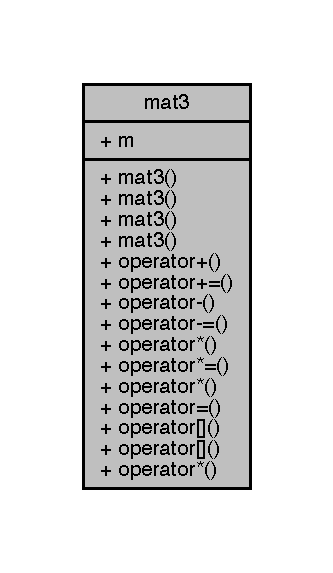
\includegraphics[width=160pt]{structmat3__coll__graph}
\end{center}
\end{figure}
\subsection*{Fonctions membres publiques}
\begin{DoxyCompactItemize}
\item 
\hyperlink{structmat3_a463027040addb1c56fe84c91b74b8d79}{mat3} ()
\item 
\hyperlink{structmat3_ae70cff0193ac1f77c61df7a2f4c00ef6}{mat3} (int)
\item 
\hyperlink{structmat3_ad5f393d1a6f7986207680e54e81f9906}{mat3} (float a, float b, float c, float d, float e, float f, float g, float h, float i)
\item 
\hyperlink{structmat3_aa761860db5b00723649f4751b34df952}{mat3} (const \hyperlink{structmat3}{mat3} \&)
\item 
\hyperlink{structmat3}{mat3} \hyperlink{structmat3_af00e96acb51cd53669a5d3a169d96e65}{operator+} (const \hyperlink{structmat3}{mat3} \&) const 
\item 
\hyperlink{structmat3}{mat3} \& \hyperlink{structmat3_a51c6ec6fd44fcd36022441064f6c285d}{operator+=} (const \hyperlink{structmat3}{mat3} \&)
\item 
\hyperlink{structmat3}{mat3} \hyperlink{structmat3_aa4a3e2abd71f23304e1069d3da0d60c0}{operator-\/} (const \hyperlink{structmat3}{mat3} \&) const 
\item 
\hyperlink{structmat3}{mat3} \& \hyperlink{structmat3_a1718976498fb7eddf36bbfebe76c0731}{operator-\/=} (const \hyperlink{structmat3}{mat3} \&)
\item 
\hyperlink{structmat3}{mat3} \hyperlink{structmat3_ab7b1c00fe3bfe66e48066f03a7c99cf5}{operator$\ast$} (const float) const 
\item 
\hyperlink{structmat3}{mat3} \& \hyperlink{structmat3_a782476876e4828df805c118734cef45f}{operator$\ast$=} (const float)
\item 
\hyperlink{structmat3}{mat3} \hyperlink{structmat3_affc4320ad21bf2276b32da8d96006a08}{operator$\ast$} (const \hyperlink{structmat3}{mat3} \&) const 
\item 
\hyperlink{structmat3}{mat3} \& \hyperlink{structmat3_aecf76e04b3d56cc333129fef2a832bb6}{operator=} (const \hyperlink{structmat3}{mat3} \&)
\item 
float \& \hyperlink{structmat3_afabeddfb3c711e2b0f806d9d8fa0534c}{operator\mbox{[}$\,$\mbox{]}} (int)
\item 
float \hyperlink{structmat3_ad61ce758d2b8def99daa43bded003023}{operator\mbox{[}$\,$\mbox{]}} (int) const 
\item 
\hyperlink{structvec3}{vec3} \hyperlink{structmat3_a08a5fd5fdb707a1ffe11b4e2c8b76beb}{operator$\ast$} (const \hyperlink{structvec3}{vec3} \&) const 
\end{DoxyCompactItemize}
\subsection*{Attributs publics}
\begin{DoxyCompactItemize}
\item 
float \hyperlink{structmat3_af5c67cec8668816c844bfd3f097f9eb2}{m} \mbox{[}9\mbox{]}
\end{DoxyCompactItemize}


\subsection{Documentation des constructeurs et destructeur}
\hypertarget{structmat3_a463027040addb1c56fe84c91b74b8d79}{\index{mat3@{mat3}!mat3@{mat3}}
\index{mat3@{mat3}!mat3@{mat3}}
\subsubsection[{mat3}]{\setlength{\rightskip}{0pt plus 5cm}mat3\+::mat3 (
\begin{DoxyParamCaption}
{}
\end{DoxyParamCaption}
)}}\label{structmat3_a463027040addb1c56fe84c91b74b8d79}


Voici le graphe des appelants de cette fonction \+:
\nopagebreak
\begin{figure}[H]
\begin{center}
\leavevmode
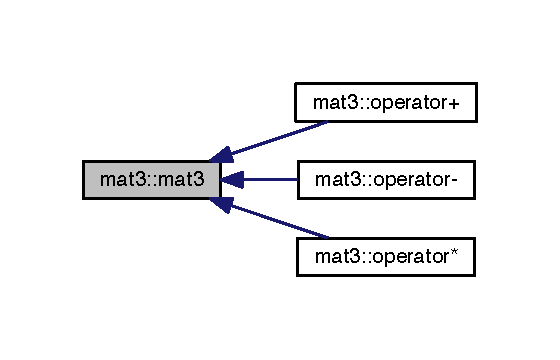
\includegraphics[width=269pt]{structmat3_a463027040addb1c56fe84c91b74b8d79_icgraph}
\end{center}
\end{figure}


\hypertarget{structmat3_ae70cff0193ac1f77c61df7a2f4c00ef6}{\index{mat3@{mat3}!mat3@{mat3}}
\index{mat3@{mat3}!mat3@{mat3}}
\subsubsection[{mat3}]{\setlength{\rightskip}{0pt plus 5cm}mat3\+::mat3 (
\begin{DoxyParamCaption}
\item[{int}]{}
\end{DoxyParamCaption}
)}}\label{structmat3_ae70cff0193ac1f77c61df7a2f4c00ef6}
\hypertarget{structmat3_ad5f393d1a6f7986207680e54e81f9906}{\index{mat3@{mat3}!mat3@{mat3}}
\index{mat3@{mat3}!mat3@{mat3}}
\subsubsection[{mat3}]{\setlength{\rightskip}{0pt plus 5cm}mat3\+::mat3 (
\begin{DoxyParamCaption}
\item[{float}]{a, }
\item[{float}]{b, }
\item[{float}]{c, }
\item[{float}]{d, }
\item[{float}]{e, }
\item[{float}]{f, }
\item[{float}]{g, }
\item[{float}]{h, }
\item[{float}]{i}
\end{DoxyParamCaption}
)}}\label{structmat3_ad5f393d1a6f7986207680e54e81f9906}
\hypertarget{structmat3_aa761860db5b00723649f4751b34df952}{\index{mat3@{mat3}!mat3@{mat3}}
\index{mat3@{mat3}!mat3@{mat3}}
\subsubsection[{mat3}]{\setlength{\rightskip}{0pt plus 5cm}mat3\+::mat3 (
\begin{DoxyParamCaption}
\item[{const {\bf mat3} \&}]{mm}
\end{DoxyParamCaption}
)}}\label{structmat3_aa761860db5b00723649f4751b34df952}


\subsection{Documentation des fonctions membres}
\hypertarget{structmat3_ab7b1c00fe3bfe66e48066f03a7c99cf5}{\index{mat3@{mat3}!operator$\ast$@{operator$\ast$}}
\index{operator$\ast$@{operator$\ast$}!mat3@{mat3}}
\subsubsection[{operator$\ast$}]{\setlength{\rightskip}{0pt plus 5cm}{\bf mat3} mat3\+::operator$\ast$ (
\begin{DoxyParamCaption}
\item[{const float}]{t}
\end{DoxyParamCaption}
) const}}\label{structmat3_ab7b1c00fe3bfe66e48066f03a7c99cf5}


Voici le graphe d'appel pour cette fonction \+:
\nopagebreak
\begin{figure}[H]
\begin{center}
\leavevmode
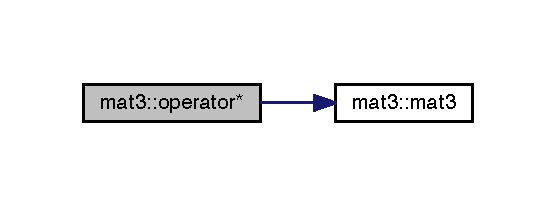
\includegraphics[width=267pt]{structmat3_ab7b1c00fe3bfe66e48066f03a7c99cf5_cgraph}
\end{center}
\end{figure}


\hypertarget{structmat3_affc4320ad21bf2276b32da8d96006a08}{\index{mat3@{mat3}!operator$\ast$@{operator$\ast$}}
\index{operator$\ast$@{operator$\ast$}!mat3@{mat3}}
\subsubsection[{operator$\ast$}]{\setlength{\rightskip}{0pt plus 5cm}{\bf mat3} mat3\+::operator$\ast$ (
\begin{DoxyParamCaption}
\item[{const {\bf mat3} \&}]{mm}
\end{DoxyParamCaption}
) const}}\label{structmat3_affc4320ad21bf2276b32da8d96006a08}


Voici le graphe d'appel pour cette fonction \+:
\nopagebreak
\begin{figure}[H]
\begin{center}
\leavevmode
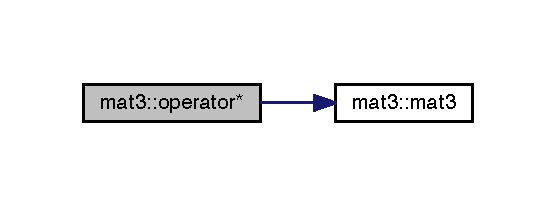
\includegraphics[width=267pt]{structmat3_affc4320ad21bf2276b32da8d96006a08_cgraph}
\end{center}
\end{figure}


\hypertarget{structmat3_a08a5fd5fdb707a1ffe11b4e2c8b76beb}{\index{mat3@{mat3}!operator$\ast$@{operator$\ast$}}
\index{operator$\ast$@{operator$\ast$}!mat3@{mat3}}
\subsubsection[{operator$\ast$}]{\setlength{\rightskip}{0pt plus 5cm}{\bf vec3} mat3\+::operator$\ast$ (
\begin{DoxyParamCaption}
\item[{const {\bf vec3} \&}]{vv}
\end{DoxyParamCaption}
) const}}\label{structmat3_a08a5fd5fdb707a1ffe11b4e2c8b76beb}
\hypertarget{structmat3_a782476876e4828df805c118734cef45f}{\index{mat3@{mat3}!operator$\ast$=@{operator$\ast$=}}
\index{operator$\ast$=@{operator$\ast$=}!mat3@{mat3}}
\subsubsection[{operator$\ast$=}]{\setlength{\rightskip}{0pt plus 5cm}{\bf mat3} \& mat3\+::operator$\ast$= (
\begin{DoxyParamCaption}
\item[{const float}]{t}
\end{DoxyParamCaption}
)}}\label{structmat3_a782476876e4828df805c118734cef45f}
\hypertarget{structmat3_af00e96acb51cd53669a5d3a169d96e65}{\index{mat3@{mat3}!operator+@{operator+}}
\index{operator+@{operator+}!mat3@{mat3}}
\subsubsection[{operator+}]{\setlength{\rightskip}{0pt plus 5cm}{\bf mat3} mat3\+::operator+ (
\begin{DoxyParamCaption}
\item[{const {\bf mat3} \&}]{mm}
\end{DoxyParamCaption}
) const}}\label{structmat3_af00e96acb51cd53669a5d3a169d96e65}


Voici le graphe d'appel pour cette fonction \+:
\nopagebreak
\begin{figure}[H]
\begin{center}
\leavevmode
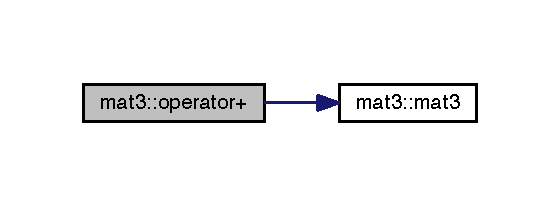
\includegraphics[width=269pt]{structmat3_af00e96acb51cd53669a5d3a169d96e65_cgraph}
\end{center}
\end{figure}


\hypertarget{structmat3_a51c6ec6fd44fcd36022441064f6c285d}{\index{mat3@{mat3}!operator+=@{operator+=}}
\index{operator+=@{operator+=}!mat3@{mat3}}
\subsubsection[{operator+=}]{\setlength{\rightskip}{0pt plus 5cm}{\bf mat3} \& mat3\+::operator+= (
\begin{DoxyParamCaption}
\item[{const {\bf mat3} \&}]{mm}
\end{DoxyParamCaption}
)}}\label{structmat3_a51c6ec6fd44fcd36022441064f6c285d}
\hypertarget{structmat3_aa4a3e2abd71f23304e1069d3da0d60c0}{\index{mat3@{mat3}!operator-\/@{operator-\/}}
\index{operator-\/@{operator-\/}!mat3@{mat3}}
\subsubsection[{operator-\/}]{\setlength{\rightskip}{0pt plus 5cm}{\bf mat3} mat3\+::operator-\/ (
\begin{DoxyParamCaption}
\item[{const {\bf mat3} \&}]{mm}
\end{DoxyParamCaption}
) const}}\label{structmat3_aa4a3e2abd71f23304e1069d3da0d60c0}


Voici le graphe d'appel pour cette fonction \+:
\nopagebreak
\begin{figure}[H]
\begin{center}
\leavevmode
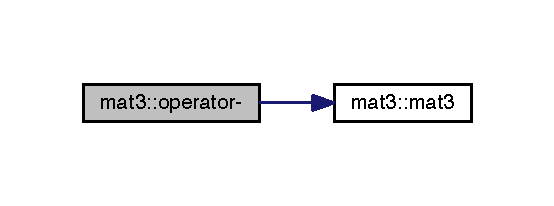
\includegraphics[width=266pt]{structmat3_aa4a3e2abd71f23304e1069d3da0d60c0_cgraph}
\end{center}
\end{figure}


\hypertarget{structmat3_a1718976498fb7eddf36bbfebe76c0731}{\index{mat3@{mat3}!operator-\/=@{operator-\/=}}
\index{operator-\/=@{operator-\/=}!mat3@{mat3}}
\subsubsection[{operator-\/=}]{\setlength{\rightskip}{0pt plus 5cm}{\bf mat3} \& mat3\+::operator-\/= (
\begin{DoxyParamCaption}
\item[{const {\bf mat3} \&}]{mm}
\end{DoxyParamCaption}
)}}\label{structmat3_a1718976498fb7eddf36bbfebe76c0731}
\hypertarget{structmat3_aecf76e04b3d56cc333129fef2a832bb6}{\index{mat3@{mat3}!operator=@{operator=}}
\index{operator=@{operator=}!mat3@{mat3}}
\subsubsection[{operator=}]{\setlength{\rightskip}{0pt plus 5cm}{\bf mat3} \& mat3\+::operator= (
\begin{DoxyParamCaption}
\item[{const {\bf mat3} \&}]{mm}
\end{DoxyParamCaption}
)}}\label{structmat3_aecf76e04b3d56cc333129fef2a832bb6}
\hypertarget{structmat3_afabeddfb3c711e2b0f806d9d8fa0534c}{\index{mat3@{mat3}!operator\mbox{[}$\,$\mbox{]}@{operator[]}}
\index{operator\mbox{[}$\,$\mbox{]}@{operator[]}!mat3@{mat3}}
\subsubsection[{operator[]}]{\setlength{\rightskip}{0pt plus 5cm}float \& mat3\+::operator\mbox{[}$\,$\mbox{]} (
\begin{DoxyParamCaption}
\item[{int}]{i}
\end{DoxyParamCaption}
)}}\label{structmat3_afabeddfb3c711e2b0f806d9d8fa0534c}
\hypertarget{structmat3_ad61ce758d2b8def99daa43bded003023}{\index{mat3@{mat3}!operator\mbox{[}$\,$\mbox{]}@{operator[]}}
\index{operator\mbox{[}$\,$\mbox{]}@{operator[]}!mat3@{mat3}}
\subsubsection[{operator[]}]{\setlength{\rightskip}{0pt plus 5cm}float mat3\+::operator\mbox{[}$\,$\mbox{]} (
\begin{DoxyParamCaption}
\item[{int}]{i}
\end{DoxyParamCaption}
) const}}\label{structmat3_ad61ce758d2b8def99daa43bded003023}


\subsection{Documentation des données membres}
\hypertarget{structmat3_af5c67cec8668816c844bfd3f097f9eb2}{\index{mat3@{mat3}!m@{m}}
\index{m@{m}!mat3@{mat3}}
\subsubsection[{m}]{\setlength{\rightskip}{0pt plus 5cm}float mat3\+::m\mbox{[}9\mbox{]}}}\label{structmat3_af5c67cec8668816c844bfd3f097f9eb2}


La documentation de cette structure a été générée à partir des fichiers suivants \+:\begin{DoxyCompactItemize}
\item 
\hyperlink{helper_8hpp}{helper.\+hpp}\item 
\hyperlink{helper_8cpp}{helper.\+cpp}\end{DoxyCompactItemize}

\hypertarget{structmat4}{\section{Référence de la structure mat4}
\label{structmat4}\index{mat4@{mat4}}
}


{\ttfamily \#include $<$helper.\+hpp$>$}



Graphe de collaboration de mat4\+:
\nopagebreak
\begin{figure}[H]
\begin{center}
\leavevmode
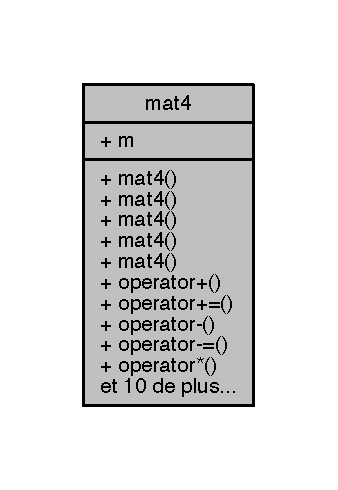
\includegraphics[width=162pt]{structmat4__coll__graph}
\end{center}
\end{figure}
\subsection*{Fonctions membres publiques}
\begin{DoxyCompactItemize}
\item 
\hyperlink{structmat4_acf3f0c37ff5c16e8fb1bfdde2bf87a0f}{mat4} ()
\item 
\hyperlink{structmat4_abbb345d8e90b7f5520a2854e4d171fad}{mat4} (int)
\item 
\hyperlink{structmat4_a9064945e550426ca0cbdc783abc159e3}{mat4} (float a, float b, float c, float d, float e, float f, float g, float h, float i, float j, float k, float l, float \hyperlink{structmat4_ab424bc8677a83f16bd30f4eaaecb6d3a}{m}, float n, float o, float p)
\item 
\hyperlink{structmat4_af9f2c48595cc3ef77b7264b6e1b80a9f}{mat4} (float $\ast$v)
\item 
\hyperlink{structmat4_a073e199b47525502781e3c36ef032dfb}{mat4} (const \hyperlink{structmat4}{mat4} \&)
\item 
\hyperlink{structmat4}{mat4} \hyperlink{structmat4_a1e09ab23f48d22eacf7480be5a6cea87}{operator+} (const \hyperlink{structmat4}{mat4} \&) const 
\item 
\hyperlink{structmat4}{mat4} \& \hyperlink{structmat4_a350e999ece6a2de198453342051887d5}{operator+=} (const \hyperlink{structmat4}{mat4} \&)
\item 
\hyperlink{structmat4}{mat4} \hyperlink{structmat4_a2ad7a60d812142642531b0ac06bf1c8e}{operator-\/} (const \hyperlink{structmat4}{mat4} \&) const 
\item 
\hyperlink{structmat4}{mat4} \& \hyperlink{structmat4_ac132dfe2e95f489dbd7164d91b535d7b}{operator-\/=} (const \hyperlink{structmat4}{mat4} \&)
\item 
\hyperlink{structmat4}{mat4} \hyperlink{structmat4_adfe86534dfda83be41334feaff6a9584}{operator$\ast$} (const float) const 
\item 
\hyperlink{structmat4}{mat4} \& \hyperlink{structmat4_ad0826521db3c90c1b3aba01c0e36d26e}{operator$\ast$=} (const float)
\item 
\hyperlink{structmat4}{mat4} \hyperlink{structmat4_a7cabd070852d9ccb840b20a6e4e492c2}{operator$\ast$} (const \hyperlink{structmat4}{mat4} \&) const 
\item 
\hyperlink{structmat4}{mat4} \& \hyperlink{structmat4_a480d75ddc6c5b4cd52f96eb9bde7966a}{operator$\ast$=} (const \hyperlink{structmat4}{mat4} \&)
\item 
\hyperlink{structmat4}{mat4} \& \hyperlink{structmat4_a22fc670708db72d05fc55bf02ad9bdcf}{operator=} (const \hyperlink{structmat4}{mat4} \&)
\item 
float \& \hyperlink{structmat4_ad4b21a373faeca027b94e0dce7f215ed}{operator\mbox{[}$\,$\mbox{]}} (int)
\item 
float \hyperlink{structmat4_a6fc70cc7bcabfc7127aef3a2a5cffaaa}{operator\mbox{[}$\,$\mbox{]}} (int) const 
\item 
\hyperlink{structvec4}{vec4} \hyperlink{structmat4_a74d5aa4c7f0bb9b4061551fbb06c120e}{operator$\ast$} (const \hyperlink{structvec4}{vec4} \&) const 
\item 
\hyperlink{structmat4}{mat4} \hyperlink{structmat4_aab816366c2233c95eac70b2eab11e8e2}{transpose} () const 
\item 
\hyperlink{structmat4}{mat4} \hyperlink{structmat4_a90efa7f6bcd321d1433629c8e6c09af3}{inverse} () const 
\item 
float \hyperlink{structmat4_a80b3a218af52e2cdcc5a216bfaa064b7}{det} () const 
\end{DoxyCompactItemize}
\subsection*{Attributs publics}
\begin{DoxyCompactItemize}
\item 
float \hyperlink{structmat4_ab424bc8677a83f16bd30f4eaaecb6d3a}{m} \mbox{[}16\mbox{]}
\end{DoxyCompactItemize}


\subsection{Documentation des constructeurs et destructeur}
\hypertarget{structmat4_acf3f0c37ff5c16e8fb1bfdde2bf87a0f}{\index{mat4@{mat4}!mat4@{mat4}}
\index{mat4@{mat4}!mat4@{mat4}}
\subsubsection[{mat4}]{\setlength{\rightskip}{0pt plus 5cm}mat4\+::mat4 (
\begin{DoxyParamCaption}
{}
\end{DoxyParamCaption}
)}}\label{structmat4_acf3f0c37ff5c16e8fb1bfdde2bf87a0f}


Voici le graphe des appelants de cette fonction \+:
\nopagebreak
\begin{figure}[H]
\begin{center}
\leavevmode
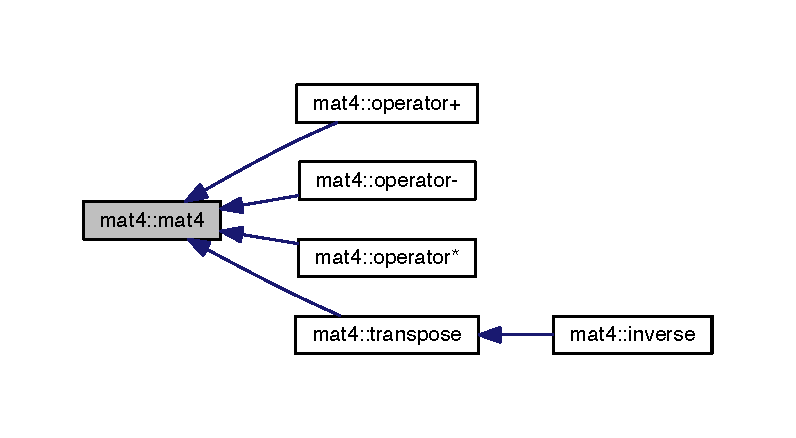
\includegraphics[width=350pt]{structmat4_acf3f0c37ff5c16e8fb1bfdde2bf87a0f_icgraph}
\end{center}
\end{figure}


\hypertarget{structmat4_abbb345d8e90b7f5520a2854e4d171fad}{\index{mat4@{mat4}!mat4@{mat4}}
\index{mat4@{mat4}!mat4@{mat4}}
\subsubsection[{mat4}]{\setlength{\rightskip}{0pt plus 5cm}mat4\+::mat4 (
\begin{DoxyParamCaption}
\item[{int}]{}
\end{DoxyParamCaption}
)}}\label{structmat4_abbb345d8e90b7f5520a2854e4d171fad}
\hypertarget{structmat4_a9064945e550426ca0cbdc783abc159e3}{\index{mat4@{mat4}!mat4@{mat4}}
\index{mat4@{mat4}!mat4@{mat4}}
\subsubsection[{mat4}]{\setlength{\rightskip}{0pt plus 5cm}mat4\+::mat4 (
\begin{DoxyParamCaption}
\item[{float}]{a, }
\item[{float}]{b, }
\item[{float}]{c, }
\item[{float}]{d, }
\item[{float}]{e, }
\item[{float}]{f, }
\item[{float}]{g, }
\item[{float}]{h, }
\item[{float}]{i, }
\item[{float}]{j, }
\item[{float}]{k, }
\item[{float}]{l, }
\item[{float}]{m, }
\item[{float}]{n, }
\item[{float}]{o, }
\item[{float}]{p}
\end{DoxyParamCaption}
)}}\label{structmat4_a9064945e550426ca0cbdc783abc159e3}
\hypertarget{structmat4_af9f2c48595cc3ef77b7264b6e1b80a9f}{\index{mat4@{mat4}!mat4@{mat4}}
\index{mat4@{mat4}!mat4@{mat4}}
\subsubsection[{mat4}]{\setlength{\rightskip}{0pt plus 5cm}mat4\+::mat4 (
\begin{DoxyParamCaption}
\item[{float $\ast$}]{v}
\end{DoxyParamCaption}
)}}\label{structmat4_af9f2c48595cc3ef77b7264b6e1b80a9f}
\hypertarget{structmat4_a073e199b47525502781e3c36ef032dfb}{\index{mat4@{mat4}!mat4@{mat4}}
\index{mat4@{mat4}!mat4@{mat4}}
\subsubsection[{mat4}]{\setlength{\rightskip}{0pt plus 5cm}mat4\+::mat4 (
\begin{DoxyParamCaption}
\item[{const {\bf mat4} \&}]{mm}
\end{DoxyParamCaption}
)}}\label{structmat4_a073e199b47525502781e3c36ef032dfb}


\subsection{Documentation des fonctions membres}
\hypertarget{structmat4_a80b3a218af52e2cdcc5a216bfaa064b7}{\index{mat4@{mat4}!det@{det}}
\index{det@{det}!mat4@{mat4}}
\subsubsection[{det}]{\setlength{\rightskip}{0pt plus 5cm}float mat4\+::det (
\begin{DoxyParamCaption}
{}
\end{DoxyParamCaption}
) const}}\label{structmat4_a80b3a218af52e2cdcc5a216bfaa064b7}


Voici le graphe des appelants de cette fonction \+:
\nopagebreak
\begin{figure}[H]
\begin{center}
\leavevmode
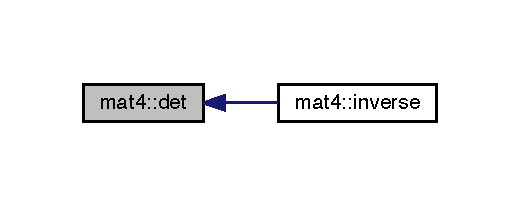
\includegraphics[width=250pt]{structmat4_a80b3a218af52e2cdcc5a216bfaa064b7_icgraph}
\end{center}
\end{figure}


\hypertarget{structmat4_a90efa7f6bcd321d1433629c8e6c09af3}{\index{mat4@{mat4}!inverse@{inverse}}
\index{inverse@{inverse}!mat4@{mat4}}
\subsubsection[{inverse}]{\setlength{\rightskip}{0pt plus 5cm}{\bf mat4} mat4\+::inverse (
\begin{DoxyParamCaption}
{}
\end{DoxyParamCaption}
) const}}\label{structmat4_a90efa7f6bcd321d1433629c8e6c09af3}


Voici le graphe d'appel pour cette fonction \+:
\nopagebreak
\begin{figure}[H]
\begin{center}
\leavevmode
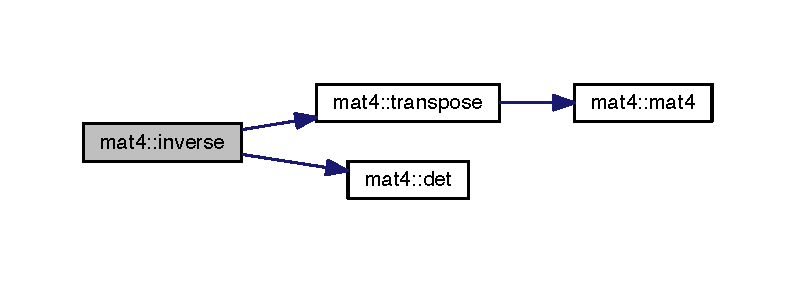
\includegraphics[width=350pt]{structmat4_a90efa7f6bcd321d1433629c8e6c09af3_cgraph}
\end{center}
\end{figure}


\hypertarget{structmat4_adfe86534dfda83be41334feaff6a9584}{\index{mat4@{mat4}!operator$\ast$@{operator$\ast$}}
\index{operator$\ast$@{operator$\ast$}!mat4@{mat4}}
\subsubsection[{operator$\ast$}]{\setlength{\rightskip}{0pt plus 5cm}{\bf mat4} mat4\+::operator$\ast$ (
\begin{DoxyParamCaption}
\item[{const float}]{t}
\end{DoxyParamCaption}
) const}}\label{structmat4_adfe86534dfda83be41334feaff6a9584}


Voici le graphe d'appel pour cette fonction \+:
\nopagebreak
\begin{figure}[H]
\begin{center}
\leavevmode
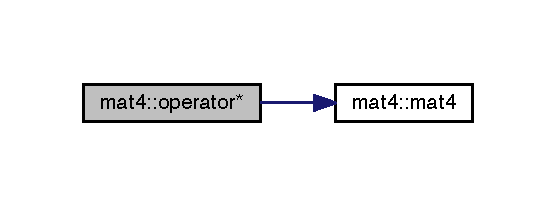
\includegraphics[width=267pt]{structmat4_adfe86534dfda83be41334feaff6a9584_cgraph}
\end{center}
\end{figure}


\hypertarget{structmat4_a7cabd070852d9ccb840b20a6e4e492c2}{\index{mat4@{mat4}!operator$\ast$@{operator$\ast$}}
\index{operator$\ast$@{operator$\ast$}!mat4@{mat4}}
\subsubsection[{operator$\ast$}]{\setlength{\rightskip}{0pt plus 5cm}{\bf mat4} mat4\+::operator$\ast$ (
\begin{DoxyParamCaption}
\item[{const {\bf mat4} \&}]{mm}
\end{DoxyParamCaption}
) const}}\label{structmat4_a7cabd070852d9ccb840b20a6e4e492c2}


Voici le graphe d'appel pour cette fonction \+:
\nopagebreak
\begin{figure}[H]
\begin{center}
\leavevmode
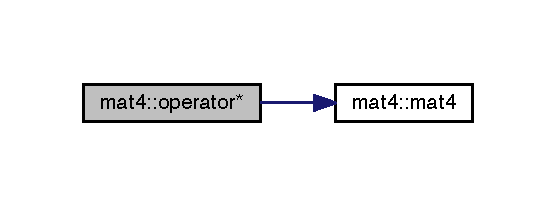
\includegraphics[width=267pt]{structmat4_a7cabd070852d9ccb840b20a6e4e492c2_cgraph}
\end{center}
\end{figure}


\hypertarget{structmat4_a74d5aa4c7f0bb9b4061551fbb06c120e}{\index{mat4@{mat4}!operator$\ast$@{operator$\ast$}}
\index{operator$\ast$@{operator$\ast$}!mat4@{mat4}}
\subsubsection[{operator$\ast$}]{\setlength{\rightskip}{0pt plus 5cm}{\bf vec4} mat4\+::operator$\ast$ (
\begin{DoxyParamCaption}
\item[{const {\bf vec4} \&}]{vv}
\end{DoxyParamCaption}
) const}}\label{structmat4_a74d5aa4c7f0bb9b4061551fbb06c120e}
\hypertarget{structmat4_ad0826521db3c90c1b3aba01c0e36d26e}{\index{mat4@{mat4}!operator$\ast$=@{operator$\ast$=}}
\index{operator$\ast$=@{operator$\ast$=}!mat4@{mat4}}
\subsubsection[{operator$\ast$=}]{\setlength{\rightskip}{0pt plus 5cm}{\bf mat4} \& mat4\+::operator$\ast$= (
\begin{DoxyParamCaption}
\item[{const float}]{t}
\end{DoxyParamCaption}
)}}\label{structmat4_ad0826521db3c90c1b3aba01c0e36d26e}
\hypertarget{structmat4_a480d75ddc6c5b4cd52f96eb9bde7966a}{\index{mat4@{mat4}!operator$\ast$=@{operator$\ast$=}}
\index{operator$\ast$=@{operator$\ast$=}!mat4@{mat4}}
\subsubsection[{operator$\ast$=}]{\setlength{\rightskip}{0pt plus 5cm}{\bf mat4} \& mat4\+::operator$\ast$= (
\begin{DoxyParamCaption}
\item[{const {\bf mat4} \&}]{mm}
\end{DoxyParamCaption}
)}}\label{structmat4_a480d75ddc6c5b4cd52f96eb9bde7966a}
\hypertarget{structmat4_a1e09ab23f48d22eacf7480be5a6cea87}{\index{mat4@{mat4}!operator+@{operator+}}
\index{operator+@{operator+}!mat4@{mat4}}
\subsubsection[{operator+}]{\setlength{\rightskip}{0pt plus 5cm}{\bf mat4} mat4\+::operator+ (
\begin{DoxyParamCaption}
\item[{const {\bf mat4} \&}]{mm}
\end{DoxyParamCaption}
) const}}\label{structmat4_a1e09ab23f48d22eacf7480be5a6cea87}


Voici le graphe d'appel pour cette fonction \+:
\nopagebreak
\begin{figure}[H]
\begin{center}
\leavevmode
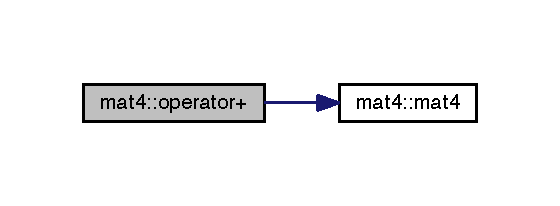
\includegraphics[width=269pt]{structmat4_a1e09ab23f48d22eacf7480be5a6cea87_cgraph}
\end{center}
\end{figure}


\hypertarget{structmat4_a350e999ece6a2de198453342051887d5}{\index{mat4@{mat4}!operator+=@{operator+=}}
\index{operator+=@{operator+=}!mat4@{mat4}}
\subsubsection[{operator+=}]{\setlength{\rightskip}{0pt plus 5cm}{\bf mat4} \& mat4\+::operator+= (
\begin{DoxyParamCaption}
\item[{const {\bf mat4} \&}]{mm}
\end{DoxyParamCaption}
)}}\label{structmat4_a350e999ece6a2de198453342051887d5}
\hypertarget{structmat4_a2ad7a60d812142642531b0ac06bf1c8e}{\index{mat4@{mat4}!operator-\/@{operator-\/}}
\index{operator-\/@{operator-\/}!mat4@{mat4}}
\subsubsection[{operator-\/}]{\setlength{\rightskip}{0pt plus 5cm}{\bf mat4} mat4\+::operator-\/ (
\begin{DoxyParamCaption}
\item[{const {\bf mat4} \&}]{mm}
\end{DoxyParamCaption}
) const}}\label{structmat4_a2ad7a60d812142642531b0ac06bf1c8e}


Voici le graphe d'appel pour cette fonction \+:
\nopagebreak
\begin{figure}[H]
\begin{center}
\leavevmode
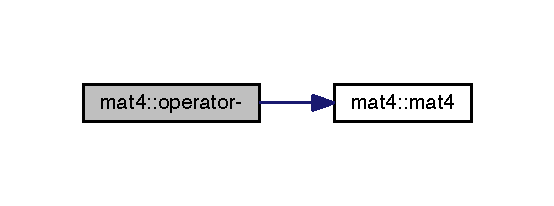
\includegraphics[width=266pt]{structmat4_a2ad7a60d812142642531b0ac06bf1c8e_cgraph}
\end{center}
\end{figure}


\hypertarget{structmat4_ac132dfe2e95f489dbd7164d91b535d7b}{\index{mat4@{mat4}!operator-\/=@{operator-\/=}}
\index{operator-\/=@{operator-\/=}!mat4@{mat4}}
\subsubsection[{operator-\/=}]{\setlength{\rightskip}{0pt plus 5cm}{\bf mat4} \& mat4\+::operator-\/= (
\begin{DoxyParamCaption}
\item[{const {\bf mat4} \&}]{mm}
\end{DoxyParamCaption}
)}}\label{structmat4_ac132dfe2e95f489dbd7164d91b535d7b}
\hypertarget{structmat4_a22fc670708db72d05fc55bf02ad9bdcf}{\index{mat4@{mat4}!operator=@{operator=}}
\index{operator=@{operator=}!mat4@{mat4}}
\subsubsection[{operator=}]{\setlength{\rightskip}{0pt plus 5cm}{\bf mat4} \& mat4\+::operator= (
\begin{DoxyParamCaption}
\item[{const {\bf mat4} \&}]{mm}
\end{DoxyParamCaption}
)}}\label{structmat4_a22fc670708db72d05fc55bf02ad9bdcf}
\hypertarget{structmat4_ad4b21a373faeca027b94e0dce7f215ed}{\index{mat4@{mat4}!operator\mbox{[}$\,$\mbox{]}@{operator[]}}
\index{operator\mbox{[}$\,$\mbox{]}@{operator[]}!mat4@{mat4}}
\subsubsection[{operator[]}]{\setlength{\rightskip}{0pt plus 5cm}float \& mat4\+::operator\mbox{[}$\,$\mbox{]} (
\begin{DoxyParamCaption}
\item[{int}]{i}
\end{DoxyParamCaption}
)}}\label{structmat4_ad4b21a373faeca027b94e0dce7f215ed}
\hypertarget{structmat4_a6fc70cc7bcabfc7127aef3a2a5cffaaa}{\index{mat4@{mat4}!operator\mbox{[}$\,$\mbox{]}@{operator[]}}
\index{operator\mbox{[}$\,$\mbox{]}@{operator[]}!mat4@{mat4}}
\subsubsection[{operator[]}]{\setlength{\rightskip}{0pt plus 5cm}float mat4\+::operator\mbox{[}$\,$\mbox{]} (
\begin{DoxyParamCaption}
\item[{int}]{i}
\end{DoxyParamCaption}
) const}}\label{structmat4_a6fc70cc7bcabfc7127aef3a2a5cffaaa}
\hypertarget{structmat4_aab816366c2233c95eac70b2eab11e8e2}{\index{mat4@{mat4}!transpose@{transpose}}
\index{transpose@{transpose}!mat4@{mat4}}
\subsubsection[{transpose}]{\setlength{\rightskip}{0pt plus 5cm}{\bf mat4} mat4\+::transpose (
\begin{DoxyParamCaption}
{}
\end{DoxyParamCaption}
) const}}\label{structmat4_aab816366c2233c95eac70b2eab11e8e2}


Voici le graphe d'appel pour cette fonction \+:
\nopagebreak
\begin{figure}[H]
\begin{center}
\leavevmode
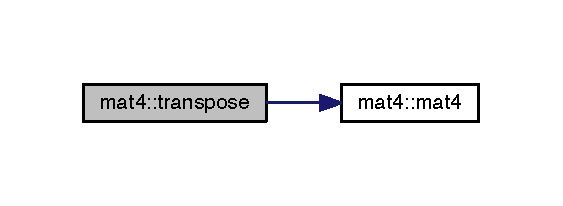
\includegraphics[width=270pt]{structmat4_aab816366c2233c95eac70b2eab11e8e2_cgraph}
\end{center}
\end{figure}




Voici le graphe des appelants de cette fonction \+:
\nopagebreak
\begin{figure}[H]
\begin{center}
\leavevmode
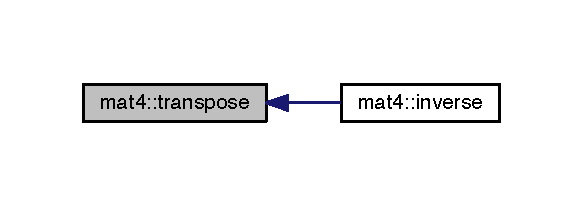
\includegraphics[width=280pt]{structmat4_aab816366c2233c95eac70b2eab11e8e2_icgraph}
\end{center}
\end{figure}




\subsection{Documentation des données membres}
\hypertarget{structmat4_ab424bc8677a83f16bd30f4eaaecb6d3a}{\index{mat4@{mat4}!m@{m}}
\index{m@{m}!mat4@{mat4}}
\subsubsection[{m}]{\setlength{\rightskip}{0pt plus 5cm}float mat4\+::m\mbox{[}16\mbox{]}}}\label{structmat4_ab424bc8677a83f16bd30f4eaaecb6d3a}


La documentation de cette structure a été générée à partir des fichiers suivants \+:\begin{DoxyCompactItemize}
\item 
\hyperlink{helper_8hpp}{helper.\+hpp}\item 
\hyperlink{helper_8cpp}{helper.\+cpp}\end{DoxyCompactItemize}

\hypertarget{class_material}{\section{Material Class Reference}
\label{class_material}\index{Material@{Material}}
}


Matériaux pour la \hyperlink{class_scene}{Scene}.  




{\ttfamily \#include $<$material.\+hpp$>$}

Inheritance diagram for Material\+:\begin{figure}[H]
\begin{center}
\leavevmode
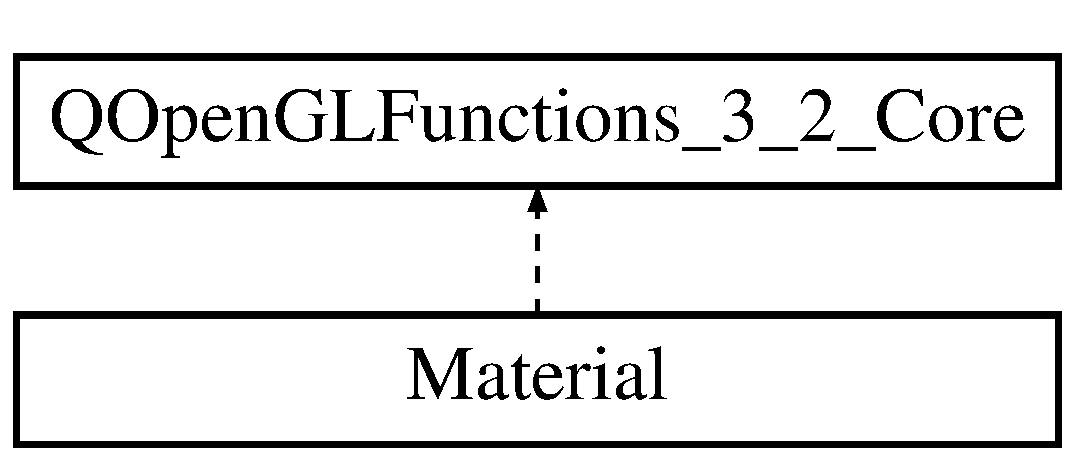
\includegraphics[height=2.000000cm]{class_material}
\end{center}
\end{figure}
\subsection*{Public Member Functions}
\begin{DoxyCompactItemize}
\item 
\hyperlink{class_material_a1692495b8e704a0ab17701365eb34b0f}{Material} (\hyperlink{structvec3}{vec3} ambient=\hyperlink{structvec3}{vec3}(0.\+2, 0.\+2, 0.\+2), \hyperlink{structvec3}{vec3} diffuse=\hyperlink{structvec3}{vec3}(0.\+8, 0.\+8, 0.\+8), \hyperlink{structvec3}{vec3} specular=\hyperlink{structvec3}{vec3}(0.\+8, 0.\+8, 0.\+8), float \hyperlink{class_material_a9a938aa96f0d5a5dc4d17d43cfd4b42b}{shininess}=0.\+0f, vec3 emissive=vec3(0.\+0, 0.\+0, 0.\+0))
\begin{DoxyCompactList}\small\item\em Constructeur. \end{DoxyCompactList}\item 
\hyperlink{class_material_a2c19452d71f54075df8f5405b03129f4}{$\sim$\+Material} ()
\begin{DoxyCompactList}\small\item\em Destructeur. \end{DoxyCompactList}\item 
void \hyperlink{class_material_a2ab92e03d9c90294cd28fff9b6a8cde0}{set} (G\+Lenum type, \hyperlink{structvec4}{vec4} value)
\begin{DoxyCompactList}\small\item\em Met à jour la composante du matériaux. \end{DoxyCompactList}\item 
void \hyperlink{class_material_a4f2227a6fb3f12c8618e399f93ab492c}{add\+Texture} (const Q\+String \&tex\+File, const Q\+String \&type)
\begin{DoxyCompactList}\small\item\em Charge une texture et l'associe à un slot. \end{DoxyCompactList}\item 
void \hyperlink{class_material_a3de47a95f13dc6f6306493516814762c}{set} (float \hyperlink{class_material_a9a938aa96f0d5a5dc4d17d43cfd4b42b}{shininess})
\begin{DoxyCompactList}\small\item\em Met à jour la shniness du \hyperlink{class_material}{Material}. \end{DoxyCompactList}\item 
\hyperlink{structvec3}{vec3} \hyperlink{class_material_a6b4b32cf23cbba3988becd840471a51c}{get} (G\+Lenum type) const 
\begin{DoxyCompactList}\small\item\em Récupère la valeur d'un champ. \end{DoxyCompactList}\item 
\hyperlink{structvec3}{vec3} \& \hyperlink{class_material_a229d118ec5602033bafbc1212a7b72ce}{get} (G\+Lenum type)
\begin{DoxyCompactList}\small\item\em Récupère la valeur d'un champ. \end{DoxyCompactList}\item 
float \hyperlink{class_material_a9a938aa96f0d5a5dc4d17d43cfd4b42b}{shininess} () const 
\begin{DoxyCompactList}\small\item\em Valeur du shininess. \end{DoxyCompactList}\item 
bool \hyperlink{class_material_a5a489f2fa09381b917c6bc3244e02877}{has\+Texture} (unsigned char type) const 
\item 
bool \hyperlink{class_material_aa07bc322b6904dd4ccf61620a0eb703c}{has\+Diffuse\+Texture} () const 
\item 
bool \hyperlink{class_material_ab1d0beef91e6149c0ebfc6c82b977889}{has\+Specular\+Texture} () const 
\item 
bool \hyperlink{class_material_a9bfe6c055d9af6f3ef029b62cc57e6a1}{has\+Normal\+Texture} () const 
\item 
Q\+String \hyperlink{class_material_a9305ced3fea7ab22cd25877e14cfb53c}{get\+Diffuse\+Texture\+Name} () const 
\begin{DoxyCompactList}\small\item\em Retourne le path de la texture diffuse. \end{DoxyCompactList}\item 
Q\+String \hyperlink{class_material_a0f33deb2e971506b9382d1ece4ff2fa6}{get\+Specular\+Texture\+Name} () const 
\begin{DoxyCompactList}\small\item\em Retourne le path de la texture spéculaire. \end{DoxyCompactList}\item 
Q\+String \hyperlink{class_material_ae72d423e9f07b3cc0388854e0ad2c1ca}{get\+Normal\+Texture\+Name} () const 
\begin{DoxyCompactList}\small\item\em Retourne le path de la normal map. \end{DoxyCompactList}\item 
void \hyperlink{class_material_a3f43fe7bcfa721fd8156adb151adf45c}{update} ()
\begin{DoxyCompactList}\small\item\em Met à jour le \hyperlink{class_material}{Material} courant dans le shader actif. \end{DoxyCompactList}\item 
bool \hyperlink{class_material_a3641da3931be722a809b13f882e2a703}{is\+From\+X\+M\+L} () const 
\begin{DoxyCompactList}\small\item\em Indique si le \hyperlink{class_material}{Material} a été chargé depuis le X\+M\+L ou pas. \end{DoxyCompactList}\item 
void \hyperlink{class_material_a806be90008bdccd18e0d657ac75ef61c}{from\+X\+M\+L} (bool b)
\begin{DoxyCompactList}\small\item\em Indique si le \hyperlink{class_material}{Material} est issu ou non du X\+M\+L. \end{DoxyCompactList}\end{DoxyCompactItemize}
\subsection*{Static Public Member Functions}
\begin{DoxyCompactItemize}
\item 
static void \hyperlink{class_material_ab350dd584b850dfc3e0c52201b5699e0}{clear} ()
\begin{DoxyCompactList}\small\item\em Libère les textures chargées. \end{DoxyCompactList}\end{DoxyCompactItemize}
\subsection*{Private Attributes}
\begin{DoxyCompactItemize}
\item 
\hyperlink{structvec3}{vec3} \hyperlink{class_material_a4c29044a3f7e8008eb3a0666c4ce09b9}{\+\_\+ambient}
\item 
\hyperlink{structvec3}{vec3} \hyperlink{class_material_a402005729d7d5a147d51dfcd691d2ffa}{\+\_\+diffuse}
\item 
\hyperlink{structvec3}{vec3} \hyperlink{class_material_af3e2839f5a712fba28111e00783af70f}{\+\_\+specular}
\item 
float \hyperlink{class_material_ae3f666b9de93b770232ebb5b1b3ee47e}{\+\_\+shininess}
\item 
\hyperlink{structvec3}{vec3} \hyperlink{class_material_a7c2eb5e499b3f46ec6e9d62f02653879}{\+\_\+emissive}
\item 
Q\+Open\+G\+L\+Texture $\ast$ \hyperlink{class_material_a522d07896a1363e987d09d8e4b66c156}{\+\_\+diffuse\+\_\+texture}
\item 
Q\+Open\+G\+L\+Texture $\ast$ \hyperlink{class_material_a15711d6d794b6ea122e38738fa73ba8a}{\+\_\+specular\+\_\+texture}
\item 
Q\+Open\+G\+L\+Texture $\ast$ \hyperlink{class_material_add78622071d92485dd37dbd1934453b3}{\+\_\+normal\+\_\+texture}
\item 
bool \hyperlink{class_material_a3a262cfbb40e19f79b29c61386e76f95}{\+\_\+from\+X\+M\+L}
\end{DoxyCompactItemize}
\subsection*{Static Private Attributes}
\begin{DoxyCompactItemize}
\item 
static Q\+Map$<$ Q\+String, \\*
Q\+Open\+G\+L\+Texture $\ast$ $>$ \hyperlink{class_material_a9f91b9fda835fed049df5c6959043623}{\+\_\+textures\+Loaded}
\end{DoxyCompactItemize}
\subsection*{Friends}
\begin{DoxyCompactItemize}
\item 
Q\+Debug \hyperlink{class_material_a6796ee577479f67459444fcd552e6c05}{operator$<$$<$} (Q\+Debug dbg, const \hyperlink{class_material}{Material} \&m)
\end{DoxyCompactItemize}


\subsection{Detailed Description}
Matériaux pour la \hyperlink{class_scene}{Scene}. 

Contient les informations nécessaire à la gestion d'un material pour la scène 

\subsection{Constructor \& Destructor Documentation}
\hypertarget{class_material_a1692495b8e704a0ab17701365eb34b0f}{\index{Material@{Material}!Material@{Material}}
\index{Material@{Material}!Material@{Material}}
\subsubsection[{Material}]{\setlength{\rightskip}{0pt plus 5cm}Material\+::\+Material (
\begin{DoxyParamCaption}
\item[{{\bf vec3}}]{ambient = {\ttfamily {\bf vec3}(0.2,~0.2,~0.2)}, }
\item[{{\bf vec3}}]{diffuse = {\ttfamily {\bf vec3}(0.8,~0.8,~0.8)}, }
\item[{{\bf vec3}}]{specular = {\ttfamily {\bf vec3}(0.8,~0.8,~0.8)}, }
\item[{float}]{shininess = {\ttfamily 0.0f}, }
\item[{{\bf vec3}}]{emissive = {\ttfamily {\bf vec3}(0.0,~0.0,~0.0)}}
\end{DoxyParamCaption}
)}}\label{class_material_a1692495b8e704a0ab17701365eb34b0f}


Constructeur. 

\begin{DoxyWarning}{Warning}
composante emissive pas encore gérée 
\end{DoxyWarning}
\hypertarget{class_material_a2c19452d71f54075df8f5405b03129f4}{\index{Material@{Material}!````~Material@{$\sim$\+Material}}
\index{````~Material@{$\sim$\+Material}!Material@{Material}}
\subsubsection[{$\sim$\+Material}]{\setlength{\rightskip}{0pt plus 5cm}Material\+::$\sim$\+Material (
\begin{DoxyParamCaption}
{}
\end{DoxyParamCaption}
)}}\label{class_material_a2c19452d71f54075df8f5405b03129f4}


Destructeur. 

\begin{DoxyRefDesc}{Todo}
\item[\hyperlink{todo__todo000003}{Todo}]Gérer libération de la texture quand plus utilisée \end{DoxyRefDesc}


\subsection{Member Function Documentation}
\hypertarget{class_material_a4f2227a6fb3f12c8618e399f93ab492c}{\index{Material@{Material}!add\+Texture@{add\+Texture}}
\index{add\+Texture@{add\+Texture}!Material@{Material}}
\subsubsection[{add\+Texture}]{\setlength{\rightskip}{0pt plus 5cm}void Material\+::add\+Texture (
\begin{DoxyParamCaption}
\item[{const Q\+String \&}]{tex\+File, }
\item[{const Q\+String \&}]{type}
\end{DoxyParamCaption}
)}}\label{class_material_a4f2227a6fb3f12c8618e399f93ab492c}


Charge une texture et l'associe à un slot. 

Charge une texture et l'associe à un slot pour le passage au shader


\begin{DoxyParams}{Parameters}
{\em tex\+File} & fichier de texture à charger \\
\hline
{\em int} & indice que la texture doit occuper \\
\hline
\end{DoxyParams}
\begin{DoxyWarning}{Warning}
Ecrase la texture à l'indice choisie 
\end{DoxyWarning}
\hypertarget{class_material_ab350dd584b850dfc3e0c52201b5699e0}{\index{Material@{Material}!clear@{clear}}
\index{clear@{clear}!Material@{Material}}
\subsubsection[{clear}]{\setlength{\rightskip}{0pt plus 5cm}void Material\+::clear (
\begin{DoxyParamCaption}
{}
\end{DoxyParamCaption}
)\hspace{0.3cm}{\ttfamily [static]}}}\label{class_material_ab350dd584b850dfc3e0c52201b5699e0}


Libère les textures chargées. 

\hypertarget{class_material_a806be90008bdccd18e0d657ac75ef61c}{\index{Material@{Material}!from\+X\+M\+L@{from\+X\+M\+L}}
\index{from\+X\+M\+L@{from\+X\+M\+L}!Material@{Material}}
\subsubsection[{from\+X\+M\+L}]{\setlength{\rightskip}{0pt plus 5cm}void Material\+::from\+X\+M\+L (
\begin{DoxyParamCaption}
\item[{bool}]{b}
\end{DoxyParamCaption}
)\hspace{0.3cm}{\ttfamily [inline]}}}\label{class_material_a806be90008bdccd18e0d657ac75ef61c}


Indique si le \hyperlink{class_material}{Material} est issu ou non du X\+M\+L. 

\hypertarget{class_material_a6b4b32cf23cbba3988becd840471a51c}{\index{Material@{Material}!get@{get}}
\index{get@{get}!Material@{Material}}
\subsubsection[{get}]{\setlength{\rightskip}{0pt plus 5cm}{\bf vec3} Material\+::get (
\begin{DoxyParamCaption}
\item[{G\+Lenum}]{type}
\end{DoxyParamCaption}
) const}}\label{class_material_a6b4b32cf23cbba3988becd840471a51c}


Récupère la valeur d'un champ. 


\begin{DoxyParams}{Parameters}
{\em type} & doit être parmis G\+L\+\_\+\+A\+M\+B\+I\+E\+N\+T, G\+L\+\_\+\+D\+I\+F\+F\+U\+S\+E, G\+L\+\_\+\+S\+P\+E\+C\+U\+L\+A\+R \\
\hline
\end{DoxyParams}
\begin{DoxyReturn}{Returns}
dans le cas de G\+L\+\_\+\+A\+M\+B\+I\+E\+N\+T, G\+L\+\_\+\+D\+I\+F\+F\+U\+S\+E, G\+L\+\_\+\+S\+P\+E\+C\+U\+L\+A\+R retourne un \hyperlink{structvec3}{vec3} correspondant à la composante, retourne \hyperlink{helper_8hpp_a8d45e9fbe94ddf3c3291116b8fce15c5}{vec4()} autrement 
\end{DoxyReturn}
\hypertarget{class_material_a229d118ec5602033bafbc1212a7b72ce}{\index{Material@{Material}!get@{get}}
\index{get@{get}!Material@{Material}}
\subsubsection[{get}]{\setlength{\rightskip}{0pt plus 5cm}{\bf vec3} \& Material\+::get (
\begin{DoxyParamCaption}
\item[{G\+Lenum}]{type}
\end{DoxyParamCaption}
)}}\label{class_material_a229d118ec5602033bafbc1212a7b72ce}


Récupère la valeur d'un champ. 


\begin{DoxyParams}{Parameters}
{\em type} & doit être parmis G\+L\+\_\+\+A\+M\+B\+I\+E\+N\+T, G\+L\+\_\+\+D\+I\+F\+F\+U\+S\+E, G\+L\+\_\+\+S\+P\+E\+C\+U\+L\+A\+R \\
\hline
\end{DoxyParams}
\begin{DoxyReturn}{Returns}
dans le cas de G\+L\+\_\+\+A\+M\+B\+I\+E\+N\+T, G\+L\+\_\+\+D\+I\+F\+F\+U\+S\+E, G\+L\+\_\+\+S\+P\+E\+C\+U\+L\+A\+R retourne un \hyperlink{structvec3}{vec3} correspondant à la composante, retourne \hyperlink{helper_8hpp_a8d45e9fbe94ddf3c3291116b8fce15c5}{vec4()} autrement 
\end{DoxyReturn}
\hypertarget{class_material_a9305ced3fea7ab22cd25877e14cfb53c}{\index{Material@{Material}!get\+Diffuse\+Texture\+Name@{get\+Diffuse\+Texture\+Name}}
\index{get\+Diffuse\+Texture\+Name@{get\+Diffuse\+Texture\+Name}!Material@{Material}}
\subsubsection[{get\+Diffuse\+Texture\+Name}]{\setlength{\rightskip}{0pt plus 5cm}Q\+String Material\+::get\+Diffuse\+Texture\+Name (
\begin{DoxyParamCaption}
{}
\end{DoxyParamCaption}
) const}}\label{class_material_a9305ced3fea7ab22cd25877e14cfb53c}


Retourne le path de la texture diffuse. 

\begin{DoxyReturn}{Returns}
nom de la texture diffuse 
\end{DoxyReturn}
\hypertarget{class_material_ae72d423e9f07b3cc0388854e0ad2c1ca}{\index{Material@{Material}!get\+Normal\+Texture\+Name@{get\+Normal\+Texture\+Name}}
\index{get\+Normal\+Texture\+Name@{get\+Normal\+Texture\+Name}!Material@{Material}}
\subsubsection[{get\+Normal\+Texture\+Name}]{\setlength{\rightskip}{0pt plus 5cm}Q\+String Material\+::get\+Normal\+Texture\+Name (
\begin{DoxyParamCaption}
{}
\end{DoxyParamCaption}
) const}}\label{class_material_ae72d423e9f07b3cc0388854e0ad2c1ca}


Retourne le path de la normal map. 

\begin{DoxyReturn}{Returns}
nom de la normal map 
\end{DoxyReturn}
\hypertarget{class_material_a0f33deb2e971506b9382d1ece4ff2fa6}{\index{Material@{Material}!get\+Specular\+Texture\+Name@{get\+Specular\+Texture\+Name}}
\index{get\+Specular\+Texture\+Name@{get\+Specular\+Texture\+Name}!Material@{Material}}
\subsubsection[{get\+Specular\+Texture\+Name}]{\setlength{\rightskip}{0pt plus 5cm}Q\+String Material\+::get\+Specular\+Texture\+Name (
\begin{DoxyParamCaption}
{}
\end{DoxyParamCaption}
) const}}\label{class_material_a0f33deb2e971506b9382d1ece4ff2fa6}


Retourne le path de la texture spéculaire. 

\begin{DoxyReturn}{Returns}
nom de la texture spéculaire 
\end{DoxyReturn}
\hypertarget{class_material_aa07bc322b6904dd4ccf61620a0eb703c}{\index{Material@{Material}!has\+Diffuse\+Texture@{has\+Diffuse\+Texture}}
\index{has\+Diffuse\+Texture@{has\+Diffuse\+Texture}!Material@{Material}}
\subsubsection[{has\+Diffuse\+Texture}]{\setlength{\rightskip}{0pt plus 5cm}bool Material\+::has\+Diffuse\+Texture (
\begin{DoxyParamCaption}
{}
\end{DoxyParamCaption}
) const}}\label{class_material_aa07bc322b6904dd4ccf61620a0eb703c}
\hypertarget{class_material_a9bfe6c055d9af6f3ef029b62cc57e6a1}{\index{Material@{Material}!has\+Normal\+Texture@{has\+Normal\+Texture}}
\index{has\+Normal\+Texture@{has\+Normal\+Texture}!Material@{Material}}
\subsubsection[{has\+Normal\+Texture}]{\setlength{\rightskip}{0pt plus 5cm}bool Material\+::has\+Normal\+Texture (
\begin{DoxyParamCaption}
{}
\end{DoxyParamCaption}
) const}}\label{class_material_a9bfe6c055d9af6f3ef029b62cc57e6a1}
\hypertarget{class_material_ab1d0beef91e6149c0ebfc6c82b977889}{\index{Material@{Material}!has\+Specular\+Texture@{has\+Specular\+Texture}}
\index{has\+Specular\+Texture@{has\+Specular\+Texture}!Material@{Material}}
\subsubsection[{has\+Specular\+Texture}]{\setlength{\rightskip}{0pt plus 5cm}bool Material\+::has\+Specular\+Texture (
\begin{DoxyParamCaption}
{}
\end{DoxyParamCaption}
) const}}\label{class_material_ab1d0beef91e6149c0ebfc6c82b977889}
\hypertarget{class_material_a5a489f2fa09381b917c6bc3244e02877}{\index{Material@{Material}!has\+Texture@{has\+Texture}}
\index{has\+Texture@{has\+Texture}!Material@{Material}}
\subsubsection[{has\+Texture}]{\setlength{\rightskip}{0pt plus 5cm}bool Material\+::has\+Texture (
\begin{DoxyParamCaption}
\item[{unsigned char}]{type}
\end{DoxyParamCaption}
) const}}\label{class_material_a5a489f2fa09381b917c6bc3244e02877}
\hypertarget{class_material_a3641da3931be722a809b13f882e2a703}{\index{Material@{Material}!is\+From\+X\+M\+L@{is\+From\+X\+M\+L}}
\index{is\+From\+X\+M\+L@{is\+From\+X\+M\+L}!Material@{Material}}
\subsubsection[{is\+From\+X\+M\+L}]{\setlength{\rightskip}{0pt plus 5cm}bool Material\+::is\+From\+X\+M\+L (
\begin{DoxyParamCaption}
{}
\end{DoxyParamCaption}
) const\hspace{0.3cm}{\ttfamily [inline]}}}\label{class_material_a3641da3931be722a809b13f882e2a703}


Indique si le \hyperlink{class_material}{Material} a été chargé depuis le X\+M\+L ou pas. 

\hypertarget{class_material_a2ab92e03d9c90294cd28fff9b6a8cde0}{\index{Material@{Material}!set@{set}}
\index{set@{set}!Material@{Material}}
\subsubsection[{set}]{\setlength{\rightskip}{0pt plus 5cm}void Material\+::set (
\begin{DoxyParamCaption}
\item[{G\+Lenum}]{type, }
\item[{{\bf vec4}}]{value}
\end{DoxyParamCaption}
)}}\label{class_material_a2ab92e03d9c90294cd28fff9b6a8cde0}


Met à jour la composante du matériaux. 


\begin{DoxyParams}{Parameters}
{\em type} & la composante qui sera mise à jour, doit être parmis G\+L\+\_\+\+A\+M\+B\+I\+E\+N\+T, G\+L\+\_\+\+D\+I\+F\+F\+U\+S\+E, G\+L\+\_\+\+S\+P\+E\+C\+U\+L\+A\+R, G\+L\+\_\+\+E\+M\+I\+S\+S\+I\+O\+N \\
\hline
{\em value} & valeur \\
\hline
\end{DoxyParams}
\hypertarget{class_material_a3de47a95f13dc6f6306493516814762c}{\index{Material@{Material}!set@{set}}
\index{set@{set}!Material@{Material}}
\subsubsection[{set}]{\setlength{\rightskip}{0pt plus 5cm}void Material\+::set (
\begin{DoxyParamCaption}
\item[{float}]{shininess}
\end{DoxyParamCaption}
)}}\label{class_material_a3de47a95f13dc6f6306493516814762c}


Met à jour la shniness du \hyperlink{class_material}{Material}. 


\begin{DoxyParams}{Parameters}
{\em shininess} & valeur \\
\hline
\end{DoxyParams}
\hypertarget{class_material_a9a938aa96f0d5a5dc4d17d43cfd4b42b}{\index{Material@{Material}!shininess@{shininess}}
\index{shininess@{shininess}!Material@{Material}}
\subsubsection[{shininess}]{\setlength{\rightskip}{0pt plus 5cm}float Material\+::shininess (
\begin{DoxyParamCaption}
{}
\end{DoxyParamCaption}
) const}}\label{class_material_a9a938aa96f0d5a5dc4d17d43cfd4b42b}


Valeur du shininess. 

\begin{DoxyReturn}{Returns}
valeur du G\+L\+\_\+\+S\+H\+I\+N\+I\+N\+E\+S\+S 
\end{DoxyReturn}
\hypertarget{class_material_a3f43fe7bcfa721fd8156adb151adf45c}{\index{Material@{Material}!update@{update}}
\index{update@{update}!Material@{Material}}
\subsubsection[{update}]{\setlength{\rightskip}{0pt plus 5cm}void Material\+::update (
\begin{DoxyParamCaption}
{}
\end{DoxyParamCaption}
)}}\label{class_material_a3f43fe7bcfa721fd8156adb151adf45c}


Met à jour le \hyperlink{class_material}{Material} courant dans le shader actif. 



\subsection{Friends And Related Function Documentation}
\hypertarget{class_material_a6796ee577479f67459444fcd552e6c05}{\index{Material@{Material}!operator$<$$<$@{operator$<$$<$}}
\index{operator$<$$<$@{operator$<$$<$}!Material@{Material}}
\subsubsection[{operator$<$$<$}]{\setlength{\rightskip}{0pt plus 5cm}Q\+Debug operator$<$$<$ (
\begin{DoxyParamCaption}
\item[{Q\+Debug}]{dbg, }
\item[{const {\bf Material} \&}]{m}
\end{DoxyParamCaption}
)\hspace{0.3cm}{\ttfamily [friend]}}}\label{class_material_a6796ee577479f67459444fcd552e6c05}


\subsection{Member Data Documentation}
\hypertarget{class_material_a4c29044a3f7e8008eb3a0666c4ce09b9}{\index{Material@{Material}!\+\_\+ambient@{\+\_\+ambient}}
\index{\+\_\+ambient@{\+\_\+ambient}!Material@{Material}}
\subsubsection[{\+\_\+ambient}]{\setlength{\rightskip}{0pt plus 5cm}{\bf vec3} Material\+::\+\_\+ambient\hspace{0.3cm}{\ttfamily [private]}}}\label{class_material_a4c29044a3f7e8008eb3a0666c4ce09b9}
\hypertarget{class_material_a402005729d7d5a147d51dfcd691d2ffa}{\index{Material@{Material}!\+\_\+diffuse@{\+\_\+diffuse}}
\index{\+\_\+diffuse@{\+\_\+diffuse}!Material@{Material}}
\subsubsection[{\+\_\+diffuse}]{\setlength{\rightskip}{0pt plus 5cm}{\bf vec3} Material\+::\+\_\+diffuse\hspace{0.3cm}{\ttfamily [private]}}}\label{class_material_a402005729d7d5a147d51dfcd691d2ffa}
\hypertarget{class_material_a522d07896a1363e987d09d8e4b66c156}{\index{Material@{Material}!\+\_\+diffuse\+\_\+texture@{\+\_\+diffuse\+\_\+texture}}
\index{\+\_\+diffuse\+\_\+texture@{\+\_\+diffuse\+\_\+texture}!Material@{Material}}
\subsubsection[{\+\_\+diffuse\+\_\+texture}]{\setlength{\rightskip}{0pt plus 5cm}Q\+Open\+G\+L\+Texture$\ast$ Material\+::\+\_\+diffuse\+\_\+texture\hspace{0.3cm}{\ttfamily [private]}}}\label{class_material_a522d07896a1363e987d09d8e4b66c156}
\hypertarget{class_material_a7c2eb5e499b3f46ec6e9d62f02653879}{\index{Material@{Material}!\+\_\+emissive@{\+\_\+emissive}}
\index{\+\_\+emissive@{\+\_\+emissive}!Material@{Material}}
\subsubsection[{\+\_\+emissive}]{\setlength{\rightskip}{0pt plus 5cm}{\bf vec3} Material\+::\+\_\+emissive\hspace{0.3cm}{\ttfamily [private]}}}\label{class_material_a7c2eb5e499b3f46ec6e9d62f02653879}
\hypertarget{class_material_a3a262cfbb40e19f79b29c61386e76f95}{\index{Material@{Material}!\+\_\+from\+X\+M\+L@{\+\_\+from\+X\+M\+L}}
\index{\+\_\+from\+X\+M\+L@{\+\_\+from\+X\+M\+L}!Material@{Material}}
\subsubsection[{\+\_\+from\+X\+M\+L}]{\setlength{\rightskip}{0pt plus 5cm}bool Material\+::\+\_\+from\+X\+M\+L\hspace{0.3cm}{\ttfamily [private]}}}\label{class_material_a3a262cfbb40e19f79b29c61386e76f95}
\hypertarget{class_material_add78622071d92485dd37dbd1934453b3}{\index{Material@{Material}!\+\_\+normal\+\_\+texture@{\+\_\+normal\+\_\+texture}}
\index{\+\_\+normal\+\_\+texture@{\+\_\+normal\+\_\+texture}!Material@{Material}}
\subsubsection[{\+\_\+normal\+\_\+texture}]{\setlength{\rightskip}{0pt plus 5cm}Q\+Open\+G\+L\+Texture$\ast$ Material\+::\+\_\+normal\+\_\+texture\hspace{0.3cm}{\ttfamily [private]}}}\label{class_material_add78622071d92485dd37dbd1934453b3}
\hypertarget{class_material_ae3f666b9de93b770232ebb5b1b3ee47e}{\index{Material@{Material}!\+\_\+shininess@{\+\_\+shininess}}
\index{\+\_\+shininess@{\+\_\+shininess}!Material@{Material}}
\subsubsection[{\+\_\+shininess}]{\setlength{\rightskip}{0pt plus 5cm}float Material\+::\+\_\+shininess\hspace{0.3cm}{\ttfamily [private]}}}\label{class_material_ae3f666b9de93b770232ebb5b1b3ee47e}
\hypertarget{class_material_af3e2839f5a712fba28111e00783af70f}{\index{Material@{Material}!\+\_\+specular@{\+\_\+specular}}
\index{\+\_\+specular@{\+\_\+specular}!Material@{Material}}
\subsubsection[{\+\_\+specular}]{\setlength{\rightskip}{0pt plus 5cm}{\bf vec3} Material\+::\+\_\+specular\hspace{0.3cm}{\ttfamily [private]}}}\label{class_material_af3e2839f5a712fba28111e00783af70f}
\hypertarget{class_material_a15711d6d794b6ea122e38738fa73ba8a}{\index{Material@{Material}!\+\_\+specular\+\_\+texture@{\+\_\+specular\+\_\+texture}}
\index{\+\_\+specular\+\_\+texture@{\+\_\+specular\+\_\+texture}!Material@{Material}}
\subsubsection[{\+\_\+specular\+\_\+texture}]{\setlength{\rightskip}{0pt plus 5cm}Q\+Open\+G\+L\+Texture$\ast$ Material\+::\+\_\+specular\+\_\+texture\hspace{0.3cm}{\ttfamily [private]}}}\label{class_material_a15711d6d794b6ea122e38738fa73ba8a}
\hypertarget{class_material_a9f91b9fda835fed049df5c6959043623}{\index{Material@{Material}!\+\_\+textures\+Loaded@{\+\_\+textures\+Loaded}}
\index{\+\_\+textures\+Loaded@{\+\_\+textures\+Loaded}!Material@{Material}}
\subsubsection[{\+\_\+textures\+Loaded}]{\setlength{\rightskip}{0pt plus 5cm}Q\+Map$<$ Q\+String, Q\+Open\+G\+L\+Texture $\ast$ $>$ Material\+::\+\_\+textures\+Loaded\hspace{0.3cm}{\ttfamily [static]}, {\ttfamily [private]}}}\label{class_material_a9f91b9fda835fed049df5c6959043623}
Ensemble des textures déjà chargées pour réutilisation 

The documentation for this class was generated from the following files\+:\begin{DoxyCompactItemize}
\item 
scene/\hyperlink{material_8hpp}{material.\+hpp}\item 
scene/\hyperlink{material_8cpp}{material.\+cpp}\end{DoxyCompactItemize}

\hypertarget{class_mesh}{\section{Mesh Class Reference}
\label{class_mesh}\index{Mesh@{Mesh}}
}


Charge un modèle 3\+D.  




{\ttfamily \#include $<$mesh.\+hpp$>$}

Inheritance diagram for Mesh\+:\begin{figure}[H]
\begin{center}
\leavevmode
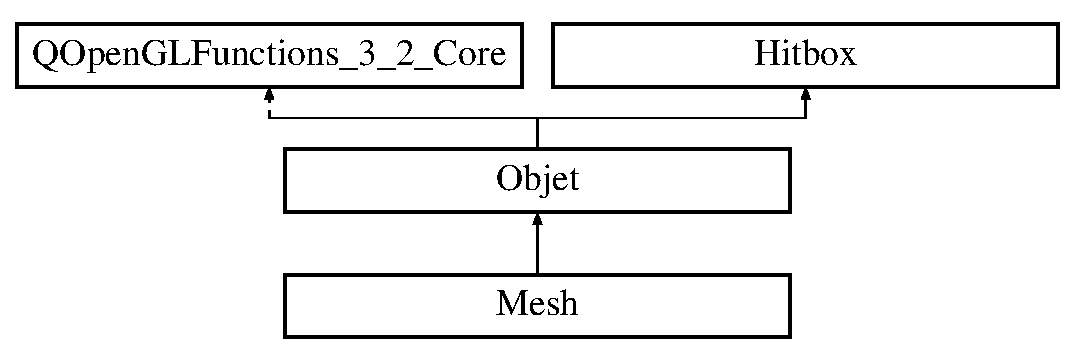
\includegraphics[height=3.000000cm]{class_mesh}
\end{center}
\end{figure}
\subsection*{Classes}
\begin{DoxyCompactItemize}
\item 
struct \hyperlink{struct_mesh_1_1_mesh_info}{Mesh\+Info}
\end{DoxyCompactItemize}
\subsection*{Public Member Functions}
\begin{DoxyCompactItemize}
\item 
\hyperlink{class_mesh_a5efe4da1a4c0971cfb037bd70304c303}{$\sim$\+Mesh} ()
\begin{DoxyCompactList}\small\item\em Destructeur. \end{DoxyCompactList}\item 
void \hyperlink{class_mesh_a996a8668fa2ca7d95d6d10744c833bc8}{draw} ()
\begin{DoxyCompactList}\small\item\em Affiche le modèle. \end{DoxyCompactList}\end{DoxyCompactItemize}
\subsection*{Protected Member Functions}
\begin{DoxyCompactItemize}
\item 
virtual \hyperlink{structvec3}{vec3} \hyperlink{class_mesh_ab1da4db267719d533521873715b9359c}{get\+P} () const 
\begin{DoxyCompactList}\small\item\em Retourne le centre de la \hyperlink{class_hitbox}{Hitbox}. \end{DoxyCompactList}\item 
virtual float \hyperlink{class_mesh_a8e0ae90ffac8c8295027d21f5af155cc}{get\+Width} () const 
\begin{DoxyCompactList}\small\item\em renvoie la demie largeur de la hitbox \end{DoxyCompactList}\item 
virtual float \hyperlink{class_mesh_a3feeb4d65973f3dc0c0e66ae95b36971}{get\+Height} () const 
\begin{DoxyCompactList}\small\item\em renvoie la demie hauteur de la hitbox \end{DoxyCompactList}\item 
virtual float \hyperlink{class_mesh_a505f44a95b363e12f6434801fe697108}{get\+Depth} () const 
\begin{DoxyCompactList}\small\item\em renvoie la demie profondeur de la hitbox \end{DoxyCompactList}\end{DoxyCompactItemize}
\subsection*{Private Member Functions}
\begin{DoxyCompactItemize}
\item 
\hyperlink{class_mesh_a2af137f1571af89172b9c102302c416b}{Mesh} ()
\begin{DoxyCompactList}\small\item\em Constructeur privé \end{DoxyCompactList}\item 
\hyperlink{class_mesh_a713cb62e7078cfd627108a0b14f72c6f}{Mesh} (const \hyperlink{class_mesh}{Mesh} \&m)
\begin{DoxyCompactList}\small\item\em Constructeur par recopie. \end{DoxyCompactList}\end{DoxyCompactItemize}
\subsection*{Static Private Member Functions}
\begin{DoxyCompactItemize}
\item 
static \hyperlink{class_mesh}{Mesh} $\ast$ \hyperlink{class_mesh_a7b405216bda9e94d64aa8a308d718cb4}{load\+Mesh} (const ai\+Mesh $\ast$scene)
\begin{DoxyCompactList}\small\item\em Charge un mesh. \end{DoxyCompactList}\end{DoxyCompactItemize}
\subsection*{Private Attributes}
\begin{DoxyCompactItemize}
\item 
\hyperlink{struct_mesh_1_1_mesh_info}{Mesh\+Info} $\ast$ \hyperlink{class_mesh_a608911b8dbff58ff769c708b8b7f2618}{\+\_\+infos}
\end{DoxyCompactItemize}
\subsection*{Friends}
\begin{DoxyCompactItemize}
\item 
class \hyperlink{class_mesh_a6db9d28bd448a131448276ee03de1e6d}{Node}
\end{DoxyCompactItemize}
\subsection*{Additional Inherited Members}


\subsection{Detailed Description}
Charge un modèle 3\+D. 

Permet la lecture de fichiers contenant des modèles 3\+D \begin{DoxyWarning}{Warning}
Tout les formats de textures ne sont pas supportés, se référé au support de Q\+Image 
\end{DoxyWarning}


\subsection{Constructor \& Destructor Documentation}
\hypertarget{class_mesh_a2af137f1571af89172b9c102302c416b}{\index{Mesh@{Mesh}!Mesh@{Mesh}}
\index{Mesh@{Mesh}!Mesh@{Mesh}}
\subsubsection[{Mesh}]{\setlength{\rightskip}{0pt plus 5cm}Mesh\+::\+Mesh (
\begin{DoxyParamCaption}
{}
\end{DoxyParamCaption}
)\hspace{0.3cm}{\ttfamily [private]}}}\label{class_mesh_a2af137f1571af89172b9c102302c416b}


Constructeur privé 

Utiliser Node\+::load(const Q\+String \& file\+Name, Scene $\ast$ scene) \begin{DoxySeeAlso}{See also}
\hyperlink{class_node_ac2140ddf8f06f8b5620e6743c945c482}{Node\+::load\+Model()} 
\end{DoxySeeAlso}
\hypertarget{class_mesh_a713cb62e7078cfd627108a0b14f72c6f}{\index{Mesh@{Mesh}!Mesh@{Mesh}}
\index{Mesh@{Mesh}!Mesh@{Mesh}}
\subsubsection[{Mesh}]{\setlength{\rightskip}{0pt plus 5cm}Mesh\+::\+Mesh (
\begin{DoxyParamCaption}
\item[{const {\bf Mesh} \&}]{m}
\end{DoxyParamCaption}
)\hspace{0.3cm}{\ttfamily [private]}}}\label{class_mesh_a713cb62e7078cfd627108a0b14f72c6f}


Constructeur par recopie. 

\hypertarget{class_mesh_a5efe4da1a4c0971cfb037bd70304c303}{\index{Mesh@{Mesh}!````~Mesh@{$\sim$\+Mesh}}
\index{````~Mesh@{$\sim$\+Mesh}!Mesh@{Mesh}}
\subsubsection[{$\sim$\+Mesh}]{\setlength{\rightskip}{0pt plus 5cm}Mesh\+::$\sim$\+Mesh (
\begin{DoxyParamCaption}
{}
\end{DoxyParamCaption}
)}}\label{class_mesh_a5efe4da1a4c0971cfb037bd70304c303}


Destructeur. 



\subsection{Member Function Documentation}
\hypertarget{class_mesh_a996a8668fa2ca7d95d6d10744c833bc8}{\index{Mesh@{Mesh}!draw@{draw}}
\index{draw@{draw}!Mesh@{Mesh}}
\subsubsection[{draw}]{\setlength{\rightskip}{0pt plus 5cm}void Mesh\+::draw (
\begin{DoxyParamCaption}
{}
\end{DoxyParamCaption}
)\hspace{0.3cm}{\ttfamily [virtual]}}}\label{class_mesh_a996a8668fa2ca7d95d6d10744c833bc8}


Affiche le modèle. 



Reimplemented from \hyperlink{class_objet_a5cc323f562964e00b947b2d908e206e7}{Objet}.

\hypertarget{class_mesh_a505f44a95b363e12f6434801fe697108}{\index{Mesh@{Mesh}!get\+Depth@{get\+Depth}}
\index{get\+Depth@{get\+Depth}!Mesh@{Mesh}}
\subsubsection[{get\+Depth}]{\setlength{\rightskip}{0pt plus 5cm}float Mesh\+::get\+Depth (
\begin{DoxyParamCaption}
{}
\end{DoxyParamCaption}
) const\hspace{0.3cm}{\ttfamily [protected]}, {\ttfamily [virtual]}}}\label{class_mesh_a505f44a95b363e12f6434801fe697108}


renvoie la demie profondeur de la hitbox 



Reimplemented from \hyperlink{class_objet_a27f49df80d4efc35530987cd8683dde0}{Objet}.

\hypertarget{class_mesh_a3feeb4d65973f3dc0c0e66ae95b36971}{\index{Mesh@{Mesh}!get\+Height@{get\+Height}}
\index{get\+Height@{get\+Height}!Mesh@{Mesh}}
\subsubsection[{get\+Height}]{\setlength{\rightskip}{0pt plus 5cm}float Mesh\+::get\+Height (
\begin{DoxyParamCaption}
{}
\end{DoxyParamCaption}
) const\hspace{0.3cm}{\ttfamily [protected]}, {\ttfamily [virtual]}}}\label{class_mesh_a3feeb4d65973f3dc0c0e66ae95b36971}


renvoie la demie hauteur de la hitbox 



Reimplemented from \hyperlink{class_objet_a05bcb1a581309e6785be09058ff68450}{Objet}.

\hypertarget{class_mesh_ab1da4db267719d533521873715b9359c}{\index{Mesh@{Mesh}!get\+P@{get\+P}}
\index{get\+P@{get\+P}!Mesh@{Mesh}}
\subsubsection[{get\+P}]{\setlength{\rightskip}{0pt plus 5cm}{\bf vec3} Mesh\+::get\+P (
\begin{DoxyParamCaption}
{}
\end{DoxyParamCaption}
) const\hspace{0.3cm}{\ttfamily [protected]}, {\ttfamily [virtual]}}}\label{class_mesh_ab1da4db267719d533521873715b9359c}


Retourne le centre de la \hyperlink{class_hitbox}{Hitbox}. 



Reimplemented from \hyperlink{class_objet_a470565255788e83680e544631b5800ff}{Objet}.

\hypertarget{class_mesh_a8e0ae90ffac8c8295027d21f5af155cc}{\index{Mesh@{Mesh}!get\+Width@{get\+Width}}
\index{get\+Width@{get\+Width}!Mesh@{Mesh}}
\subsubsection[{get\+Width}]{\setlength{\rightskip}{0pt plus 5cm}float Mesh\+::get\+Width (
\begin{DoxyParamCaption}
{}
\end{DoxyParamCaption}
) const\hspace{0.3cm}{\ttfamily [protected]}, {\ttfamily [virtual]}}}\label{class_mesh_a8e0ae90ffac8c8295027d21f5af155cc}


renvoie la demie largeur de la hitbox 



Reimplemented from \hyperlink{class_objet_ae8b213466c38b3bcaa34144cc708da65}{Objet}.

\hypertarget{class_mesh_a7b405216bda9e94d64aa8a308d718cb4}{\index{Mesh@{Mesh}!load\+Mesh@{load\+Mesh}}
\index{load\+Mesh@{load\+Mesh}!Mesh@{Mesh}}
\subsubsection[{load\+Mesh}]{\setlength{\rightskip}{0pt plus 5cm}{\bf Mesh} $\ast$ Mesh\+::load\+Mesh (
\begin{DoxyParamCaption}
\item[{const ai\+Mesh $\ast$}]{scene}
\end{DoxyParamCaption}
)\hspace{0.3cm}{\ttfamily [static]}, {\ttfamily [private]}}}\label{class_mesh_a7b405216bda9e94d64aa8a308d718cb4}


Charge un mesh. 


\begin{DoxyParams}{Parameters}
{\em scene} & scène générée par assimp\\
\hline
\end{DoxyParams}
\begin{DoxyReturn}{Returns}
un pointeur sur \hyperlink{class_mesh}{Mesh}, N\+U\+L\+L si erreur 
\end{DoxyReturn}


\subsection{Friends And Related Function Documentation}
\hypertarget{class_mesh_a6db9d28bd448a131448276ee03de1e6d}{\index{Mesh@{Mesh}!Node@{Node}}
\index{Node@{Node}!Mesh@{Mesh}}
\subsubsection[{Node}]{\setlength{\rightskip}{0pt plus 5cm}friend class {\bf Node}\hspace{0.3cm}{\ttfamily [friend]}}}\label{class_mesh_a6db9d28bd448a131448276ee03de1e6d}


\subsection{Member Data Documentation}
\hypertarget{class_mesh_a608911b8dbff58ff769c708b8b7f2618}{\index{Mesh@{Mesh}!\+\_\+infos@{\+\_\+infos}}
\index{\+\_\+infos@{\+\_\+infos}!Mesh@{Mesh}}
\subsubsection[{\+\_\+infos}]{\setlength{\rightskip}{0pt plus 5cm}{\bf Mesh\+Info}$\ast$ Mesh\+::\+\_\+infos\hspace{0.3cm}{\ttfamily [private]}}}\label{class_mesh_a608911b8dbff58ff769c708b8b7f2618}


The documentation for this class was generated from the following files\+:\begin{DoxyCompactItemize}
\item 
objets/\hyperlink{mesh_8hpp}{mesh.\+hpp}\item 
objets/\hyperlink{mesh_8cpp}{mesh.\+cpp}\end{DoxyCompactItemize}

\hypertarget{struct_mesh_1_1_mesh_info}{\section{Mesh\+:\+:Mesh\+Info Struct Reference}
\label{struct_mesh_1_1_mesh_info}\index{Mesh\+::\+Mesh\+Info@{Mesh\+::\+Mesh\+Info}}
}
\subsection*{Public Attributes}
\begin{DoxyCompactItemize}
\item 
G\+Luint \hyperlink{struct_mesh_1_1_mesh_info_af15096e0f0aa61fff7d8a1c223e547cf}{vao}
\item 
Q\+List$<$ G\+Luint $>$ \hyperlink{struct_mesh_1_1_mesh_info_ad360b326ff7424dc9b6a3f6614af895d}{vbos}
\item 
G\+Luint \hyperlink{struct_mesh_1_1_mesh_info_a8869e5c769b3895876e32bed8252dffd}{nb\+Vertices}
\item 
unsigned int \hyperlink{struct_mesh_1_1_mesh_info_a8e32fc200e5ed8af32c409cac7b17342}{nb\+References}
\end{DoxyCompactItemize}


\subsection{Member Data Documentation}
\hypertarget{struct_mesh_1_1_mesh_info_a8e32fc200e5ed8af32c409cac7b17342}{\index{Mesh\+::\+Mesh\+Info@{Mesh\+::\+Mesh\+Info}!nb\+References@{nb\+References}}
\index{nb\+References@{nb\+References}!Mesh\+::\+Mesh\+Info@{Mesh\+::\+Mesh\+Info}}
\subsubsection[{nb\+References}]{\setlength{\rightskip}{0pt plus 5cm}unsigned int Mesh\+::\+Mesh\+Info\+::nb\+References}}\label{struct_mesh_1_1_mesh_info_a8e32fc200e5ed8af32c409cac7b17342}
\hypertarget{struct_mesh_1_1_mesh_info_a8869e5c769b3895876e32bed8252dffd}{\index{Mesh\+::\+Mesh\+Info@{Mesh\+::\+Mesh\+Info}!nb\+Vertices@{nb\+Vertices}}
\index{nb\+Vertices@{nb\+Vertices}!Mesh\+::\+Mesh\+Info@{Mesh\+::\+Mesh\+Info}}
\subsubsection[{nb\+Vertices}]{\setlength{\rightskip}{0pt plus 5cm}G\+Luint Mesh\+::\+Mesh\+Info\+::nb\+Vertices}}\label{struct_mesh_1_1_mesh_info_a8869e5c769b3895876e32bed8252dffd}
\hypertarget{struct_mesh_1_1_mesh_info_af15096e0f0aa61fff7d8a1c223e547cf}{\index{Mesh\+::\+Mesh\+Info@{Mesh\+::\+Mesh\+Info}!vao@{vao}}
\index{vao@{vao}!Mesh\+::\+Mesh\+Info@{Mesh\+::\+Mesh\+Info}}
\subsubsection[{vao}]{\setlength{\rightskip}{0pt plus 5cm}G\+Luint Mesh\+::\+Mesh\+Info\+::vao}}\label{struct_mesh_1_1_mesh_info_af15096e0f0aa61fff7d8a1c223e547cf}
\hypertarget{struct_mesh_1_1_mesh_info_ad360b326ff7424dc9b6a3f6614af895d}{\index{Mesh\+::\+Mesh\+Info@{Mesh\+::\+Mesh\+Info}!vbos@{vbos}}
\index{vbos@{vbos}!Mesh\+::\+Mesh\+Info@{Mesh\+::\+Mesh\+Info}}
\subsubsection[{vbos}]{\setlength{\rightskip}{0pt plus 5cm}Q\+List$<$G\+Luint$>$ Mesh\+::\+Mesh\+Info\+::vbos}}\label{struct_mesh_1_1_mesh_info_ad360b326ff7424dc9b6a3f6614af895d}


The documentation for this struct was generated from the following file\+:\begin{DoxyCompactItemize}
\item 
objets/\hyperlink{mesh_8hpp}{mesh.\+hpp}\end{DoxyCompactItemize}

\hypertarget{class_mondock}{\section{Mondock Class Reference}
\label{class_mondock}\index{Mondock@{Mondock}}
}


{\ttfamily \#include $<$mondock.\+hpp$>$}

Inheritance diagram for Mondock\+:\begin{figure}[H]
\begin{center}
\leavevmode
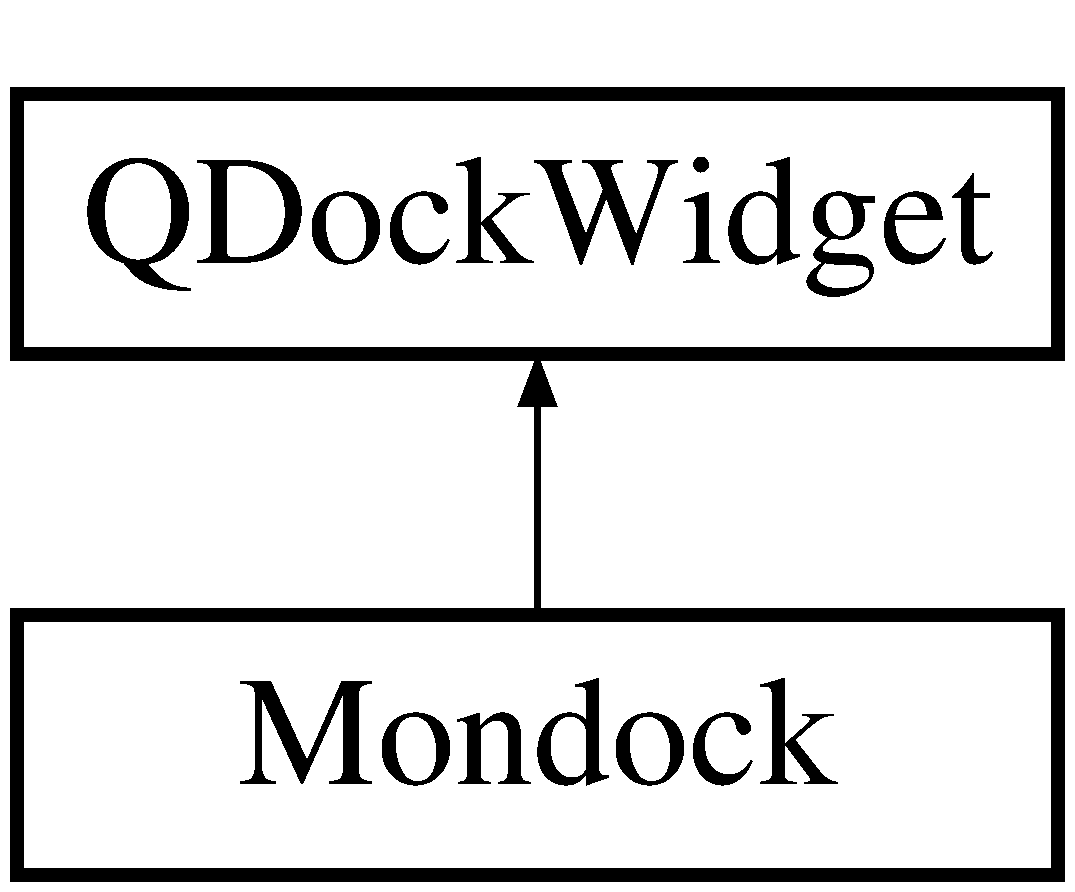
\includegraphics[height=2.000000cm]{class_mondock}
\end{center}
\end{figure}
\subsection*{Public Member Functions}
\begin{DoxyCompactItemize}
\item 
\hyperlink{class_mondock_a31297333af7c87f4f9773728db845d7f}{Mondock} (const Q\+String \&title, Q\+Widget $\ast$parent=0, Qt\+::\+Window\+Flags flags=0)
\item 
\hyperlink{class_mondock_a33aa83a1e0de9cf10380c1a5237eec7e}{$\sim$\+Mondock} ()
\end{DoxyCompactItemize}
\subsection*{Public Attributes}
\begin{DoxyCompactItemize}
\item 
\hyperlink{class_scene}{Scene} $\ast$ \hyperlink{class_mondock_ac6fd15f2143e05b554f3f936e6f1588f}{dockscene}
\item 
\hyperlink{class_light}{Light} $\ast$ \hyperlink{class_mondock_a541a241aadaf9820926b427f2d504573}{\+\_\+light}
\item 
\hyperlink{class_material}{Material} $\ast$ \hyperlink{class_mondock_ada15f5ec6dabb8728651472f5cc867a8}{\+\_\+materiaux}
\item 
\hyperlink{class_objet}{Objet} $\ast$ \hyperlink{class_mondock_a6325a3fb92643c99815b1a8025f7d401}{\+\_\+objet}
\item 
\hyperlink{class_piece}{Piece} $\ast$ \hyperlink{class_mondock_a8a9c524e7a781e45219699b15b20596f}{\+\_\+piece}
\item 
Q\+Standard\+Item\+Model $\ast$ \hyperlink{class_mondock_a3f46e1710907a9aedf250fce4ba93076}{dockmodele}
\item 
Q\+Tree\+View $\ast$ \hyperlink{class_mondock_a32e24e3ef7312fbd292740e19c3d3dcd}{dockvue}
\item 
Q\+Standard\+Item $\ast$ \hyperlink{class_mondock_ab873f19cf3a771dcb0f32480e3ea2c69}{\+\_\+itemmaterial}
\item 
Q\+Standard\+Item $\ast$ \hyperlink{class_mondock_a3de76b6bfaee199ee945f04c3c2f4c02}{\+\_\+itempiece}
\item 
Q\+Standard\+Item\+Model $\ast$ \hyperlink{class_mondock_aceda9fef8d2c8b9c88672bacbeac7988}{modelmaterial}
\end{DoxyCompactItemize}
\subsection*{Private Slots}
\begin{DoxyCompactItemize}
\item 
void \hyperlink{class_mondock_a25391f1fac7a8a46e761f2f8c9c2fdc8}{selectionlight} ()
\item 
void \hyperlink{class_mondock_a05ec25870c70f2eeba2ccdc1da44e7ca}{poslightfuncx} (double x)
\item 
void \hyperlink{class_mondock_ae8593b3cbc4c42badf600599a2e01dce}{poslightfuncy} (double x)
\item 
void \hyperlink{class_mondock_aa5ec8a8453515216ffd85961c868108f}{poslightfuncz} (double x)
\item 
void \hyperlink{class_mondock_a07685bc7db5c3346c1813e84abf8aa2f}{amblightfuncx} (int x)
\item 
void \hyperlink{class_mondock_a2397e94ee9af0a37c12b1443d70c17b6}{amblightfuncy} (int x)
\item 
void \hyperlink{class_mondock_a727e012b9b0df615ea2d585f98b00fb9}{amblightfuncz} (int x)
\item 
void \hyperlink{class_mondock_ad475a793b9d77352f2e844b22315612e}{diflightfuncx} (int x)
\item 
void \hyperlink{class_mondock_a5e60c8e141570f171d420de6f6e9af54}{diflightfuncy} (int x)
\item 
void \hyperlink{class_mondock_a4fd34f4035885b71a4d914ff85496715}{diflightfuncz} (int x)
\item 
void \hyperlink{class_mondock_ad12c449ba7b08f8430353e5fb7687e6a}{spelightfuncx} (int x)
\item 
void \hyperlink{class_mondock_ac2c735aede2c4c621f08f9c34d6a4c9c}{spelightfuncy} (int x)
\item 
void \hyperlink{class_mondock_ad626e2142ce5065af9a3bd891c825a5a}{spelightfuncz} (int x)
\item 
void \hyperlink{class_mondock_a8311bcb6b47314eba3966861c6cfe53a}{ambmaterialfuncx} (int x)
\item 
void \hyperlink{class_mondock_abab8b7116db8f4d8a45f97bbccfea28a}{ambmaterialfuncy} (int x)
\item 
void \hyperlink{class_mondock_aef75cf8b1bb4a9cf7e6f6a04ac9a6e53}{ambmaterialfuncz} (int x)
\item 
void \hyperlink{class_mondock_ab52fa4e602f9dd7686b4beaee1ae78a7}{difmaterialfuncx} (int x)
\item 
void \hyperlink{class_mondock_acb6ef6ce35644055c6782614193c0abf}{difmaterialfuncy} (int x)
\item 
void \hyperlink{class_mondock_a8ff74685d0e326198673395786ca80d4}{difmaterialfuncz} (int x)
\item 
void \hyperlink{class_mondock_ad62497d70cea045864c6f6dfa63f0a4c}{spematerialfuncx} (int x)
\item 
void \hyperlink{class_mondock_ada51acb02b3cb5d32e3982e93e2b2951}{spematerialfuncy} (int x)
\item 
void \hyperlink{class_mondock_aebe3927b8d0b1c6a703580cf69284405}{spematerialfuncz} (int x)
\item 
void \hyperlink{class_mondock_acfe377696276e313ee29188412cdefc5}{spematerialtfunca} (int x)
\item 
void \hyperlink{class_mondock_ae7cba6de97474c812bf5f6e1f5372540}{matobjet} (const Q\+String \&text)
\item 
void \hyperlink{class_mondock_afcb87fab11d89a1a24da091153d4dbac}{pereobjet} (const Q\+String \&text)
\item 
void \hyperlink{class_mondock_a7543dea413bcfc6c79847373e99f75fc}{rotobjectx} (double x)
\item 
void \hyperlink{class_mondock_ad182d69edf7f245ade47b574813357d0}{rotobjecty} (double x)
\item 
void \hyperlink{class_mondock_a90dd35e5da95e3b29a44104f8527605b}{rotobjectz} (double x)
\item 
void \hyperlink{class_mondock_a68ab5d84182366c7231014333055d12d}{transobjectx} (double x)
\item 
void \hyperlink{class_mondock_ac6fba22518497d0b8ed04c976dd98ef3}{transobjecty} (double x)
\item 
void \hyperlink{class_mondock_a4577b03f35f3e2eaa7d1826b1a9f0ebe}{transobjectz} (double x)
\item 
void \hyperlink{class_mondock_a6978ac0641ff991c971ddbb571a8e8fd}{scaleobjectx} (double x)
\item 
void \hyperlink{class_mondock_a5d96ddec02aefd94fe519bcb9d973e4f}{scaleobjecty} (double x)
\item 
void \hyperlink{class_mondock_a1f5430731565a79314d90de605741e75}{scaleobjectz} (double x)
\item 
void \hyperlink{class_mondock_aab1b5fe42325904c90cb7ea01d20dda3}{slotpositionpiecex} (int x)
\item 
void \hyperlink{class_mondock_aa9b2f07da91515f13c0dc217d24357ba}{slotpositionpiecey} (int x)
\item 
void \hyperlink{class_mondock_a655881c708869d768f1488d6fa066dc6}{slotpositionpiecez} (int x)
\end{DoxyCompactItemize}
\subsection*{Private Member Functions}
\begin{DoxyCompactItemize}
\item 
void \hyperlink{class_mondock_aea9fc6ea30f9958ac3a747552ecbed17}{traitementlumiere} ()
\item 
void \hyperlink{class_mondock_ab482a04624f22351da70e316fe9c8d4e}{traitementmaterial} ()
\item 
void \hyperlink{class_mondock_aad20b3c5334d00fe5e69ac5872f76f4b}{traitementobjet} ()
\item 
void \hyperlink{class_mondock_a8f0d8c5f390853f482b38bbcf943447a}{traitementpiece} ()
\end{DoxyCompactItemize}
\subsection*{Private Attributes}
\begin{DoxyCompactItemize}
\item 
Q\+Item\+Selection\+Model $\ast$ \hyperlink{class_mondock_aa0a94c4bfce0d7d4f2547da10d365275}{selection}
\item 
Q\+Model\+Index \hyperlink{class_mondock_a48e5355dbb076ca71a13e42172f342ca}{index\+Element\+Selectionne}
\item 
Q\+Variant \hyperlink{class_mondock_a5a0f5cf7817eee757956874e3bec2043}{element\+Selectionne\+Parent}
\item 
Q\+Model\+Index \hyperlink{class_mondock_ac8fa555c082f94d22d369eed852f93c3}{indexlight\+Selectionne}
\item 
Q\+Variant \hyperlink{class_mondock_a35acbdbc03ccc8bd255083f8499188f5}{lightselectioner}
\item 
Q\+Model\+Index \hyperlink{class_mondock_a8816860ad6351028d8d4e5b022b2b266}{indexmaterial\+Selectionne}
\item 
Q\+Variant \hyperlink{class_mondock_a09fab02186d86e999d23b4f9c667353f}{materialselectioner}
\item 
Q\+Model\+Index \hyperlink{class_mondock_ab950bd39d928049d2788f4690ba45755}{indexpiece\+Selectionne}
\item 
Q\+Variant \hyperlink{class_mondock_acc6d9454fd6ff20be6309e30aa5053c3}{pieceselectioner}
\item 
Q\+Model\+Index \hyperlink{class_mondock_a54452b93781c23fe0e40d764b2d278fe}{indexgparent}
\item 
Q\+Variant \hyperlink{class_mondock_a3c00ae3b69dc59785835aa2d04b73392}{element\+Selectionne\+G\+Parent}
\item 
Q\+Model\+Index \hyperlink{class_mondock_ab7756e9a6862132ca6b86d4b94c834c0}{indexobjetl\+Selectionne}
\item 
Q\+Variant \hyperlink{class_mondock_aba0697efe8eb1eff576ce6599aea10f3}{objetselectioner}
\item 
Q\+Standard\+Item\+Model $\ast$ \hyperlink{class_mondock_a2560c460ea144a4e8b2300dadf8df8ed}{modelpiece}
\item 
Q\+Tab\+Widget $\ast$ \hyperlink{class_mondock_aff9f46d61c662d10837346c496160ed1}{tablight}
\item 
Q\+Widget $\ast$ \hyperlink{class_mondock_af55525ced19bade9444f69f28ceb63bb}{tablightpos}
\item 
Q\+H\+Box\+Layout $\ast$ \hyperlink{class_mondock_aa1e272ef1c0db51aac8861812e367b27}{tablightposlayout}
\item 
Q\+Double\+Spin\+Box $\ast$ \hyperlink{class_mondock_a16569a61106b1c9d6506d1d2a2600759}{lightdoublespinboxx}
\item 
Q\+Double\+Spin\+Box $\ast$ \hyperlink{class_mondock_a5829d9ba58222d9ec1905d9b81efeea2}{lightdoublespinboxy}
\item 
Q\+Double\+Spin\+Box $\ast$ \hyperlink{class_mondock_a7f9c9c2b765d28670aac280b38773ee9}{lightdoublespinboxz}
\item 
Q\+Widget $\ast$ \hyperlink{class_mondock_a7e42b87b7c1088da35395d5f1ef690d8}{tablightdif}
\item 
Q\+V\+Box\+Layout $\ast$ \hyperlink{class_mondock_a2691df29ebeefa273d759a15eb4c9f51}{tabdiflayout}
\item 
Q\+H\+Box\+Layout $\ast$ \hyperlink{class_mondock_a82bd5ea86bfd95368bdef210a807b1c4}{lightdiflayout}
\item 
Q\+Slider $\ast$ \hyperlink{class_mondock_a1d4f04858d8142be0a35b1aad9f14345}{sliderdifx}
\item 
Q\+Slider $\ast$ \hyperlink{class_mondock_a61a2ab20f30425efa13abc19241dfcb7}{sliderdify}
\item 
Q\+Slider $\ast$ \hyperlink{class_mondock_af68d00a8f6995732dc8f5861b1b64de2}{sliderdifz}
\item 
Q\+H\+Box\+Layout $\ast$ \hyperlink{class_mondock_a2cc5ecc094ac129ac7cf6c70147b8d29}{labeldiflayout}
\item 
Q\+Label $\ast$ \hyperlink{class_mondock_adc2193f6756de65b0d3a3f5a3a0e7164}{labeldifx}
\item 
Q\+Label $\ast$ \hyperlink{class_mondock_ab869df2ebba1417ef476ae6df23084f3}{labeldify}
\item 
Q\+Label $\ast$ \hyperlink{class_mondock_ac4418e6866dac5b4917ed73f43ccbcaa}{labeldifz}
\item 
Q\+Widget $\ast$ \hyperlink{class_mondock_a99dad8f1fa710a564d0e8348e992372e}{tablightspe}
\item 
Q\+V\+Box\+Layout $\ast$ \hyperlink{class_mondock_af59762fb339ae8c0821fada75433e8fb}{tabspelayout}
\item 
Q\+H\+Box\+Layout $\ast$ \hyperlink{class_mondock_a9d565bf7d99d0dc112fedc26f21abf2d}{lightspelayout}
\item 
Q\+Slider $\ast$ \hyperlink{class_mondock_abd032f6caee1a61430b8f37fdf872c55}{sliderspex}
\item 
Q\+Slider $\ast$ \hyperlink{class_mondock_ab99848143e6941f878cb9328681d7690}{sliderspey}
\item 
Q\+Slider $\ast$ \hyperlink{class_mondock_a496a2a2470c9c96599cd491608544bf6}{sliderspez}
\item 
Q\+H\+Box\+Layout $\ast$ \hyperlink{class_mondock_ad034a6a1d416711fd87e9594a33d9ae4}{labelspelayout}
\item 
Q\+Label $\ast$ \hyperlink{class_mondock_a9dcd6eacb52a58adddd1f0118dc7fc66}{labelspex}
\item 
Q\+Label $\ast$ \hyperlink{class_mondock_a51f3374b36482300513cfaa0d9e7cb44}{labelspey}
\item 
Q\+Label $\ast$ \hyperlink{class_mondock_af00a5126b8b2d537b5a46064b4d26d76}{labelspez}
\item 
Q\+Widget $\ast$ \hyperlink{class_mondock_a9033d2049c8fcdc628ef06ea8cb192ca}{tablightamb}
\item 
Q\+V\+Box\+Layout $\ast$ \hyperlink{class_mondock_a73f30ee1b770ddf08cdb854136ab4e51}{tabamblayout}
\item 
Q\+H\+Box\+Layout $\ast$ \hyperlink{class_mondock_ada46a57b4e681dc6f9420ae74f46fefc}{lightamblayout}
\item 
Q\+Slider $\ast$ \hyperlink{class_mondock_a51c280e3a1dae1f368e9028069afb424}{sliderambx}
\item 
Q\+Slider $\ast$ \hyperlink{class_mondock_ac6a5fbe64fd9a0567ae84e9ec5244fbd}{slideramby}
\item 
Q\+Slider $\ast$ \hyperlink{class_mondock_aa90503d09eeebd2f51e15a416c6424c7}{sliderambz}
\item 
Q\+H\+Box\+Layout $\ast$ \hyperlink{class_mondock_a8726f8f74256a666684740d03747ad5a}{labelamblayout}
\item 
Q\+Label $\ast$ \hyperlink{class_mondock_af77614bc15448c7488db1b12a03162f5}{labelambx}
\item 
Q\+Label $\ast$ \hyperlink{class_mondock_a467e81ae77fc44ddd9785214c64ae443}{labelamby}
\item 
Q\+Label $\ast$ \hyperlink{class_mondock_a59965e3362191562ca427aaafbffb67f}{labelambz}
\item 
Q\+Tab\+Widget $\ast$ \hyperlink{class_mondock_a85429c5714bc04dc5866983a9659f723}{tabmaterial}
\item 
Q\+Widget $\ast$ \hyperlink{class_mondock_a5b0d6245de8e0e70d7552ad035295793}{tabmaterialamb}
\item 
Q\+H\+Box\+Layout $\ast$ \hyperlink{class_mondock_a768206ca1e41a57f687e6bbbdaca3a9a}{tabmaterialamblayout}
\item 
Q\+Spin\+Box $\ast$ \hyperlink{class_mondock_a4efb6643d3bea5ac601770ed2e3b3290}{materialspinboxambx}
\item 
Q\+Spin\+Box $\ast$ \hyperlink{class_mondock_a52f12188582ccf1488a2f5f2059ec304}{materialspinboxamby}
\item 
Q\+Spin\+Box $\ast$ \hyperlink{class_mondock_a24725d21ed105e3d2fc2c2360c2581a6}{materialspinboxambz}
\item 
Q\+Widget $\ast$ \hyperlink{class_mondock_a1d05427fb146c04086803be70153d868}{tabmaterialdif}
\item 
Q\+H\+Box\+Layout $\ast$ \hyperlink{class_mondock_a346764281a416f9221d71a96cf9ce4fc}{tabmaterialdiflayout}
\item 
Q\+Spin\+Box $\ast$ \hyperlink{class_mondock_abf580ff2de20747ff28cb3af69aec147}{materialspinboxdifx}
\item 
Q\+Spin\+Box $\ast$ \hyperlink{class_mondock_ab1c4bb9e29202b1fcb3d4f2f2f7112a8}{materialspinboxdify}
\item 
Q\+Spin\+Box $\ast$ \hyperlink{class_mondock_abaa05027f2871448e35b82516e0559b8}{materialspinboxdifz}
\item 
Q\+Widget $\ast$ \hyperlink{class_mondock_a7f99e6c98995aa1e236e44be190e0fa6}{tabmaterialspe}
\item 
Q\+H\+Box\+Layout $\ast$ \hyperlink{class_mondock_a705948bf976e373b5afb90c9f0641580}{tabmaterialspelayout}
\item 
Q\+Spin\+Box $\ast$ \hyperlink{class_mondock_a964af1b06eda72c95695ff25146892ec}{materialspinboxspex}
\item 
Q\+Spin\+Box $\ast$ \hyperlink{class_mondock_a38fad0c6901791690bdedba633bc3220}{materialspinboxspey}
\item 
Q\+Spin\+Box $\ast$ \hyperlink{class_mondock_ab5e93ab98c43f314fa48b84be8098beb}{materialspinboxspez}
\item 
Q\+Spin\+Box $\ast$ \hyperlink{class_mondock_a62de223ddabe875e9406fd43b892a8a0}{materialspinboxspea}
\item 
Q\+Widget $\ast$ \hyperlink{class_mondock_af4e2b3e87db243b8813a3e71cbf9dd7d}{tabmaterialemi}
\item 
Q\+H\+Box\+Layout $\ast$ \hyperlink{class_mondock_afc37221d5733642eeeeaf93042d72dcb}{tabmaterialemilayout}
\item 
Q\+Spin\+Box $\ast$ \hyperlink{class_mondock_a003c7eff97a356c6dc6d7f892719e91f}{materialspinboxemix}
\item 
Q\+Spin\+Box $\ast$ \hyperlink{class_mondock_a92982a92a14d612a49dd027cb68b6d73}{materialspinboxemiy}
\item 
Q\+Spin\+Box $\ast$ \hyperlink{class_mondock_ab95fca34ebe4db052bab4109eaf5afd1}{materialspinboxemiz}
\item 
Q\+Tab\+Widget $\ast$ \hyperlink{class_mondock_a3f12af44327a1739e8818ee91649ebbf}{tabobjet}
\item 
Q\+Widget $\ast$ \hyperlink{class_mondock_adc331c4d8373b45e636757e12a2bd5a0}{tabobjetpropr}
\item 
Q\+V\+Box\+Layout $\ast$ \hyperlink{class_mondock_ac56ddde4fb8bc59837027ed14f8b19d8}{layouttabobjetpropr}
\item 
Q\+H\+Box\+Layout $\ast$ \hyperlink{class_mondock_a933e33341a7ad640413b19c6d811559a}{layouttabobjetproprlabel}
\item 
Q\+H\+Box\+Layout $\ast$ \hyperlink{class_mondock_a666eed2f58369dbaea12c10c9c5f4888}{layouttabobjetproprcombo}
\item 
Q\+Combo\+Box $\ast$ \hyperlink{class_mondock_ab8773b4c45e6e0e13a9bb22793e3c870}{combomaterial}
\item 
Q\+Combo\+Box $\ast$ \hyperlink{class_mondock_a32ebd1f643a5f1b9749eb4f9d4940973}{comboparent}
\item 
Q\+Label $\ast$ \hyperlink{class_mondock_ac49c211334c5b4502c99dc47ff86fe1c}{labelobjetproprmaterial}
\item 
Q\+Label $\ast$ \hyperlink{class_mondock_a4d76ec3b85d44b07f7147f5b2a7c68a7}{labelobjetproprparent}
\item 
Q\+Widget $\ast$ \hyperlink{class_mondock_a917509c60bf1cd3eff74b0bd9c606dae}{tabobjetrotation}
\item 
Q\+H\+Box\+Layout $\ast$ \hyperlink{class_mondock_ab36da4ccb733ba45b30be8c325a593d9}{layouttabobjetrotation}
\item 
Q\+Double\+Spin\+Box $\ast$ \hyperlink{class_mondock_accc1854d02d6d2a0b61297b351bd196a}{boxobjetrotationx}
\item 
Q\+Double\+Spin\+Box $\ast$ \hyperlink{class_mondock_aeeea985e7f23ebf81696648d8e0dea40}{boxobjetrotationy}
\item 
Q\+Double\+Spin\+Box $\ast$ \hyperlink{class_mondock_af722379e41c8ebc43f6068754564aa4f}{boxobjetrotationz}
\item 
Q\+Widget $\ast$ \hyperlink{class_mondock_a8eee5e642f5cb6d30635c80417576622}{tabobjettrans}
\item 
Q\+H\+Box\+Layout $\ast$ \hyperlink{class_mondock_a1776a6148557d83c98a8a05368c08eef}{layouttabobjettrans}
\item 
Q\+Double\+Spin\+Box $\ast$ \hyperlink{class_mondock_a906d6de66e15f9b964d68947ac8ee94e}{boxobjettransx}
\item 
Q\+Double\+Spin\+Box $\ast$ \hyperlink{class_mondock_a15ed0b5c13500bfad6a2b5289c5a3ddf}{boxobjettransy}
\item 
Q\+Double\+Spin\+Box $\ast$ \hyperlink{class_mondock_ab0102fb06cf68a8c70fed13550b4dcb6}{boxobjettransz}
\item 
Q\+Widget $\ast$ \hyperlink{class_mondock_a2463c02b8f4ff3f1ff23f2f72e3c0f48}{tabobjetscale}
\item 
Q\+H\+Box\+Layout $\ast$ \hyperlink{class_mondock_a7337ba165d8f7543e3469a2a25f3f062}{layouttabobjetscale}
\item 
Q\+Double\+Spin\+Box $\ast$ \hyperlink{class_mondock_a0300855d7d2e07ff9f29acfe6aabf86a}{boxobjetscalex}
\item 
Q\+Double\+Spin\+Box $\ast$ \hyperlink{class_mondock_a111e6d0603d220eafef5fe6754ee5686}{boxobjetscaley}
\item 
Q\+Double\+Spin\+Box $\ast$ \hyperlink{class_mondock_a23022e2424b108b94b9519167b702b2a}{boxobjetscalez}
\item 
Q\+Tab\+Widget $\ast$ \hyperlink{class_mondock_a5985ccaca36a0e545e6e74a84623b1a9}{tabpiece}
\item 
Q\+Widget $\ast$ \hyperlink{class_mondock_abe21ad30be63590c6ce6e18969e9f082}{widgetpiecedim}
\item 
Q\+H\+Box\+Layout $\ast$ \hyperlink{class_mondock_af9d31eb2800c5608dc9da41dcf1ca1d0}{piecedimlayout}
\item 
Q\+Spin\+Box $\ast$ \hyperlink{class_mondock_ab3829ab678beb2bc391bdb325b0beda1}{dimentionpiecex}
\item 
Q\+Spin\+Box $\ast$ \hyperlink{class_mondock_a60c16f4209470967b672f33a2c4fe67c}{dimentionpiecey}
\item 
Q\+Spin\+Box $\ast$ \hyperlink{class_mondock_ab9605a7a3ee01aec5f5b29fc111abdeb}{dimentionpiecez}
\item 
Q\+Widget $\ast$ \hyperlink{class_mondock_a960802e2aa94a22487ff03bbaa102a02}{widgetpieceposi}
\item 
Q\+H\+Box\+Layout $\ast$ \hyperlink{class_mondock_a676e96b53de7e8e4fd8f82c990b074df}{pieceposilayout}
\item 
Q\+Spin\+Box $\ast$ \hyperlink{class_mondock_ab93f251cb0119893cc7aadcd3ffb8eb1}{positionpiecex}
\item 
Q\+Spin\+Box $\ast$ \hyperlink{class_mondock_a82edda6549941e9c67700ed4562abba7}{positionpiecey}
\item 
Q\+Spin\+Box $\ast$ \hyperlink{class_mondock_ac4aa7f84daff43586674a324e0a69e24}{positionpiecez}
\end{DoxyCompactItemize}


\subsection{Constructor \& Destructor Documentation}
\hypertarget{class_mondock_a31297333af7c87f4f9773728db845d7f}{\index{Mondock@{Mondock}!Mondock@{Mondock}}
\index{Mondock@{Mondock}!Mondock@{Mondock}}
\subsubsection[{Mondock}]{\setlength{\rightskip}{0pt plus 5cm}Mondock\+::\+Mondock (
\begin{DoxyParamCaption}
\item[{const Q\+String \&}]{title, }
\item[{Q\+Widget $\ast$}]{parent = {\ttfamily 0}, }
\item[{Qt\+::\+Window\+Flags}]{flags = {\ttfamily 0}}
\end{DoxyParamCaption}
)}}\label{class_mondock_a31297333af7c87f4f9773728db845d7f}
\hypertarget{class_mondock_a33aa83a1e0de9cf10380c1a5237eec7e}{\index{Mondock@{Mondock}!````~Mondock@{$\sim$\+Mondock}}
\index{````~Mondock@{$\sim$\+Mondock}!Mondock@{Mondock}}
\subsubsection[{$\sim$\+Mondock}]{\setlength{\rightskip}{0pt plus 5cm}Mondock\+::$\sim$\+Mondock (
\begin{DoxyParamCaption}
{}
\end{DoxyParamCaption}
)}}\label{class_mondock_a33aa83a1e0de9cf10380c1a5237eec7e}


\subsection{Member Function Documentation}
\hypertarget{class_mondock_a07685bc7db5c3346c1813e84abf8aa2f}{\index{Mondock@{Mondock}!amblightfuncx@{amblightfuncx}}
\index{amblightfuncx@{amblightfuncx}!Mondock@{Mondock}}
\subsubsection[{amblightfuncx}]{\setlength{\rightskip}{0pt plus 5cm}void Mondock\+::amblightfuncx (
\begin{DoxyParamCaption}
\item[{int}]{x}
\end{DoxyParamCaption}
)\hspace{0.3cm}{\ttfamily [private]}, {\ttfamily [slot]}}}\label{class_mondock_a07685bc7db5c3346c1813e84abf8aa2f}
\hypertarget{class_mondock_a2397e94ee9af0a37c12b1443d70c17b6}{\index{Mondock@{Mondock}!amblightfuncy@{amblightfuncy}}
\index{amblightfuncy@{amblightfuncy}!Mondock@{Mondock}}
\subsubsection[{amblightfuncy}]{\setlength{\rightskip}{0pt plus 5cm}void Mondock\+::amblightfuncy (
\begin{DoxyParamCaption}
\item[{int}]{x}
\end{DoxyParamCaption}
)\hspace{0.3cm}{\ttfamily [private]}, {\ttfamily [slot]}}}\label{class_mondock_a2397e94ee9af0a37c12b1443d70c17b6}
\hypertarget{class_mondock_a727e012b9b0df615ea2d585f98b00fb9}{\index{Mondock@{Mondock}!amblightfuncz@{amblightfuncz}}
\index{amblightfuncz@{amblightfuncz}!Mondock@{Mondock}}
\subsubsection[{amblightfuncz}]{\setlength{\rightskip}{0pt plus 5cm}void Mondock\+::amblightfuncz (
\begin{DoxyParamCaption}
\item[{int}]{x}
\end{DoxyParamCaption}
)\hspace{0.3cm}{\ttfamily [private]}, {\ttfamily [slot]}}}\label{class_mondock_a727e012b9b0df615ea2d585f98b00fb9}
\hypertarget{class_mondock_a8311bcb6b47314eba3966861c6cfe53a}{\index{Mondock@{Mondock}!ambmaterialfuncx@{ambmaterialfuncx}}
\index{ambmaterialfuncx@{ambmaterialfuncx}!Mondock@{Mondock}}
\subsubsection[{ambmaterialfuncx}]{\setlength{\rightskip}{0pt plus 5cm}void Mondock\+::ambmaterialfuncx (
\begin{DoxyParamCaption}
\item[{int}]{x}
\end{DoxyParamCaption}
)\hspace{0.3cm}{\ttfamily [private]}, {\ttfamily [slot]}}}\label{class_mondock_a8311bcb6b47314eba3966861c6cfe53a}
\hypertarget{class_mondock_abab8b7116db8f4d8a45f97bbccfea28a}{\index{Mondock@{Mondock}!ambmaterialfuncy@{ambmaterialfuncy}}
\index{ambmaterialfuncy@{ambmaterialfuncy}!Mondock@{Mondock}}
\subsubsection[{ambmaterialfuncy}]{\setlength{\rightskip}{0pt plus 5cm}void Mondock\+::ambmaterialfuncy (
\begin{DoxyParamCaption}
\item[{int}]{x}
\end{DoxyParamCaption}
)\hspace{0.3cm}{\ttfamily [private]}, {\ttfamily [slot]}}}\label{class_mondock_abab8b7116db8f4d8a45f97bbccfea28a}
\hypertarget{class_mondock_aef75cf8b1bb4a9cf7e6f6a04ac9a6e53}{\index{Mondock@{Mondock}!ambmaterialfuncz@{ambmaterialfuncz}}
\index{ambmaterialfuncz@{ambmaterialfuncz}!Mondock@{Mondock}}
\subsubsection[{ambmaterialfuncz}]{\setlength{\rightskip}{0pt plus 5cm}void Mondock\+::ambmaterialfuncz (
\begin{DoxyParamCaption}
\item[{int}]{x}
\end{DoxyParamCaption}
)\hspace{0.3cm}{\ttfamily [private]}, {\ttfamily [slot]}}}\label{class_mondock_aef75cf8b1bb4a9cf7e6f6a04ac9a6e53}
\hypertarget{class_mondock_ad475a793b9d77352f2e844b22315612e}{\index{Mondock@{Mondock}!diflightfuncx@{diflightfuncx}}
\index{diflightfuncx@{diflightfuncx}!Mondock@{Mondock}}
\subsubsection[{diflightfuncx}]{\setlength{\rightskip}{0pt plus 5cm}void Mondock\+::diflightfuncx (
\begin{DoxyParamCaption}
\item[{int}]{x}
\end{DoxyParamCaption}
)\hspace{0.3cm}{\ttfamily [private]}, {\ttfamily [slot]}}}\label{class_mondock_ad475a793b9d77352f2e844b22315612e}
\hypertarget{class_mondock_a5e60c8e141570f171d420de6f6e9af54}{\index{Mondock@{Mondock}!diflightfuncy@{diflightfuncy}}
\index{diflightfuncy@{diflightfuncy}!Mondock@{Mondock}}
\subsubsection[{diflightfuncy}]{\setlength{\rightskip}{0pt plus 5cm}void Mondock\+::diflightfuncy (
\begin{DoxyParamCaption}
\item[{int}]{x}
\end{DoxyParamCaption}
)\hspace{0.3cm}{\ttfamily [private]}, {\ttfamily [slot]}}}\label{class_mondock_a5e60c8e141570f171d420de6f6e9af54}
\hypertarget{class_mondock_a4fd34f4035885b71a4d914ff85496715}{\index{Mondock@{Mondock}!diflightfuncz@{diflightfuncz}}
\index{diflightfuncz@{diflightfuncz}!Mondock@{Mondock}}
\subsubsection[{diflightfuncz}]{\setlength{\rightskip}{0pt plus 5cm}void Mondock\+::diflightfuncz (
\begin{DoxyParamCaption}
\item[{int}]{x}
\end{DoxyParamCaption}
)\hspace{0.3cm}{\ttfamily [private]}, {\ttfamily [slot]}}}\label{class_mondock_a4fd34f4035885b71a4d914ff85496715}
\hypertarget{class_mondock_ab52fa4e602f9dd7686b4beaee1ae78a7}{\index{Mondock@{Mondock}!difmaterialfuncx@{difmaterialfuncx}}
\index{difmaterialfuncx@{difmaterialfuncx}!Mondock@{Mondock}}
\subsubsection[{difmaterialfuncx}]{\setlength{\rightskip}{0pt plus 5cm}void Mondock\+::difmaterialfuncx (
\begin{DoxyParamCaption}
\item[{int}]{x}
\end{DoxyParamCaption}
)\hspace{0.3cm}{\ttfamily [private]}, {\ttfamily [slot]}}}\label{class_mondock_ab52fa4e602f9dd7686b4beaee1ae78a7}
\hypertarget{class_mondock_acb6ef6ce35644055c6782614193c0abf}{\index{Mondock@{Mondock}!difmaterialfuncy@{difmaterialfuncy}}
\index{difmaterialfuncy@{difmaterialfuncy}!Mondock@{Mondock}}
\subsubsection[{difmaterialfuncy}]{\setlength{\rightskip}{0pt plus 5cm}void Mondock\+::difmaterialfuncy (
\begin{DoxyParamCaption}
\item[{int}]{x}
\end{DoxyParamCaption}
)\hspace{0.3cm}{\ttfamily [private]}, {\ttfamily [slot]}}}\label{class_mondock_acb6ef6ce35644055c6782614193c0abf}
\hypertarget{class_mondock_a8ff74685d0e326198673395786ca80d4}{\index{Mondock@{Mondock}!difmaterialfuncz@{difmaterialfuncz}}
\index{difmaterialfuncz@{difmaterialfuncz}!Mondock@{Mondock}}
\subsubsection[{difmaterialfuncz}]{\setlength{\rightskip}{0pt plus 5cm}void Mondock\+::difmaterialfuncz (
\begin{DoxyParamCaption}
\item[{int}]{x}
\end{DoxyParamCaption}
)\hspace{0.3cm}{\ttfamily [private]}, {\ttfamily [slot]}}}\label{class_mondock_a8ff74685d0e326198673395786ca80d4}
\hypertarget{class_mondock_ae7cba6de97474c812bf5f6e1f5372540}{\index{Mondock@{Mondock}!matobjet@{matobjet}}
\index{matobjet@{matobjet}!Mondock@{Mondock}}
\subsubsection[{matobjet}]{\setlength{\rightskip}{0pt plus 5cm}void Mondock\+::matobjet (
\begin{DoxyParamCaption}
\item[{const Q\+String \&}]{text}
\end{DoxyParamCaption}
)\hspace{0.3cm}{\ttfamily [private]}, {\ttfamily [slot]}}}\label{class_mondock_ae7cba6de97474c812bf5f6e1f5372540}
\hypertarget{class_mondock_afcb87fab11d89a1a24da091153d4dbac}{\index{Mondock@{Mondock}!pereobjet@{pereobjet}}
\index{pereobjet@{pereobjet}!Mondock@{Mondock}}
\subsubsection[{pereobjet}]{\setlength{\rightskip}{0pt plus 5cm}void Mondock\+::pereobjet (
\begin{DoxyParamCaption}
\item[{const Q\+String \&}]{text}
\end{DoxyParamCaption}
)\hspace{0.3cm}{\ttfamily [private]}, {\ttfamily [slot]}}}\label{class_mondock_afcb87fab11d89a1a24da091153d4dbac}
\hypertarget{class_mondock_a05ec25870c70f2eeba2ccdc1da44e7ca}{\index{Mondock@{Mondock}!poslightfuncx@{poslightfuncx}}
\index{poslightfuncx@{poslightfuncx}!Mondock@{Mondock}}
\subsubsection[{poslightfuncx}]{\setlength{\rightskip}{0pt plus 5cm}void Mondock\+::poslightfuncx (
\begin{DoxyParamCaption}
\item[{double}]{x}
\end{DoxyParamCaption}
)\hspace{0.3cm}{\ttfamily [private]}, {\ttfamily [slot]}}}\label{class_mondock_a05ec25870c70f2eeba2ccdc1da44e7ca}
\hypertarget{class_mondock_ae8593b3cbc4c42badf600599a2e01dce}{\index{Mondock@{Mondock}!poslightfuncy@{poslightfuncy}}
\index{poslightfuncy@{poslightfuncy}!Mondock@{Mondock}}
\subsubsection[{poslightfuncy}]{\setlength{\rightskip}{0pt plus 5cm}void Mondock\+::poslightfuncy (
\begin{DoxyParamCaption}
\item[{double}]{x}
\end{DoxyParamCaption}
)\hspace{0.3cm}{\ttfamily [private]}, {\ttfamily [slot]}}}\label{class_mondock_ae8593b3cbc4c42badf600599a2e01dce}
\hypertarget{class_mondock_aa5ec8a8453515216ffd85961c868108f}{\index{Mondock@{Mondock}!poslightfuncz@{poslightfuncz}}
\index{poslightfuncz@{poslightfuncz}!Mondock@{Mondock}}
\subsubsection[{poslightfuncz}]{\setlength{\rightskip}{0pt plus 5cm}void Mondock\+::poslightfuncz (
\begin{DoxyParamCaption}
\item[{double}]{x}
\end{DoxyParamCaption}
)\hspace{0.3cm}{\ttfamily [private]}, {\ttfamily [slot]}}}\label{class_mondock_aa5ec8a8453515216ffd85961c868108f}
\hypertarget{class_mondock_a7543dea413bcfc6c79847373e99f75fc}{\index{Mondock@{Mondock}!rotobjectx@{rotobjectx}}
\index{rotobjectx@{rotobjectx}!Mondock@{Mondock}}
\subsubsection[{rotobjectx}]{\setlength{\rightskip}{0pt plus 5cm}void Mondock\+::rotobjectx (
\begin{DoxyParamCaption}
\item[{double}]{x}
\end{DoxyParamCaption}
)\hspace{0.3cm}{\ttfamily [private]}, {\ttfamily [slot]}}}\label{class_mondock_a7543dea413bcfc6c79847373e99f75fc}
\hypertarget{class_mondock_ad182d69edf7f245ade47b574813357d0}{\index{Mondock@{Mondock}!rotobjecty@{rotobjecty}}
\index{rotobjecty@{rotobjecty}!Mondock@{Mondock}}
\subsubsection[{rotobjecty}]{\setlength{\rightskip}{0pt plus 5cm}void Mondock\+::rotobjecty (
\begin{DoxyParamCaption}
\item[{double}]{x}
\end{DoxyParamCaption}
)\hspace{0.3cm}{\ttfamily [private]}, {\ttfamily [slot]}}}\label{class_mondock_ad182d69edf7f245ade47b574813357d0}
\hypertarget{class_mondock_a90dd35e5da95e3b29a44104f8527605b}{\index{Mondock@{Mondock}!rotobjectz@{rotobjectz}}
\index{rotobjectz@{rotobjectz}!Mondock@{Mondock}}
\subsubsection[{rotobjectz}]{\setlength{\rightskip}{0pt plus 5cm}void Mondock\+::rotobjectz (
\begin{DoxyParamCaption}
\item[{double}]{x}
\end{DoxyParamCaption}
)\hspace{0.3cm}{\ttfamily [private]}, {\ttfamily [slot]}}}\label{class_mondock_a90dd35e5da95e3b29a44104f8527605b}
\hypertarget{class_mondock_a6978ac0641ff991c971ddbb571a8e8fd}{\index{Mondock@{Mondock}!scaleobjectx@{scaleobjectx}}
\index{scaleobjectx@{scaleobjectx}!Mondock@{Mondock}}
\subsubsection[{scaleobjectx}]{\setlength{\rightskip}{0pt plus 5cm}void Mondock\+::scaleobjectx (
\begin{DoxyParamCaption}
\item[{double}]{x}
\end{DoxyParamCaption}
)\hspace{0.3cm}{\ttfamily [private]}, {\ttfamily [slot]}}}\label{class_mondock_a6978ac0641ff991c971ddbb571a8e8fd}
\hypertarget{class_mondock_a5d96ddec02aefd94fe519bcb9d973e4f}{\index{Mondock@{Mondock}!scaleobjecty@{scaleobjecty}}
\index{scaleobjecty@{scaleobjecty}!Mondock@{Mondock}}
\subsubsection[{scaleobjecty}]{\setlength{\rightskip}{0pt plus 5cm}void Mondock\+::scaleobjecty (
\begin{DoxyParamCaption}
\item[{double}]{x}
\end{DoxyParamCaption}
)\hspace{0.3cm}{\ttfamily [private]}, {\ttfamily [slot]}}}\label{class_mondock_a5d96ddec02aefd94fe519bcb9d973e4f}
\hypertarget{class_mondock_a1f5430731565a79314d90de605741e75}{\index{Mondock@{Mondock}!scaleobjectz@{scaleobjectz}}
\index{scaleobjectz@{scaleobjectz}!Mondock@{Mondock}}
\subsubsection[{scaleobjectz}]{\setlength{\rightskip}{0pt plus 5cm}void Mondock\+::scaleobjectz (
\begin{DoxyParamCaption}
\item[{double}]{x}
\end{DoxyParamCaption}
)\hspace{0.3cm}{\ttfamily [private]}, {\ttfamily [slot]}}}\label{class_mondock_a1f5430731565a79314d90de605741e75}
\hypertarget{class_mondock_a25391f1fac7a8a46e761f2f8c9c2fdc8}{\index{Mondock@{Mondock}!selectionlight@{selectionlight}}
\index{selectionlight@{selectionlight}!Mondock@{Mondock}}
\subsubsection[{selectionlight}]{\setlength{\rightskip}{0pt plus 5cm}void Mondock\+::selectionlight (
\begin{DoxyParamCaption}
{}
\end{DoxyParamCaption}
)\hspace{0.3cm}{\ttfamily [private]}, {\ttfamily [slot]}}}\label{class_mondock_a25391f1fac7a8a46e761f2f8c9c2fdc8}
\hypertarget{class_mondock_aab1b5fe42325904c90cb7ea01d20dda3}{\index{Mondock@{Mondock}!slotpositionpiecex@{slotpositionpiecex}}
\index{slotpositionpiecex@{slotpositionpiecex}!Mondock@{Mondock}}
\subsubsection[{slotpositionpiecex}]{\setlength{\rightskip}{0pt plus 5cm}void Mondock\+::slotpositionpiecex (
\begin{DoxyParamCaption}
\item[{int}]{x}
\end{DoxyParamCaption}
)\hspace{0.3cm}{\ttfamily [private]}, {\ttfamily [slot]}}}\label{class_mondock_aab1b5fe42325904c90cb7ea01d20dda3}
\hypertarget{class_mondock_aa9b2f07da91515f13c0dc217d24357ba}{\index{Mondock@{Mondock}!slotpositionpiecey@{slotpositionpiecey}}
\index{slotpositionpiecey@{slotpositionpiecey}!Mondock@{Mondock}}
\subsubsection[{slotpositionpiecey}]{\setlength{\rightskip}{0pt plus 5cm}void Mondock\+::slotpositionpiecey (
\begin{DoxyParamCaption}
\item[{int}]{x}
\end{DoxyParamCaption}
)\hspace{0.3cm}{\ttfamily [private]}, {\ttfamily [slot]}}}\label{class_mondock_aa9b2f07da91515f13c0dc217d24357ba}
\hypertarget{class_mondock_a655881c708869d768f1488d6fa066dc6}{\index{Mondock@{Mondock}!slotpositionpiecez@{slotpositionpiecez}}
\index{slotpositionpiecez@{slotpositionpiecez}!Mondock@{Mondock}}
\subsubsection[{slotpositionpiecez}]{\setlength{\rightskip}{0pt plus 5cm}void Mondock\+::slotpositionpiecez (
\begin{DoxyParamCaption}
\item[{int}]{x}
\end{DoxyParamCaption}
)\hspace{0.3cm}{\ttfamily [private]}, {\ttfamily [slot]}}}\label{class_mondock_a655881c708869d768f1488d6fa066dc6}
\hypertarget{class_mondock_ad12c449ba7b08f8430353e5fb7687e6a}{\index{Mondock@{Mondock}!spelightfuncx@{spelightfuncx}}
\index{spelightfuncx@{spelightfuncx}!Mondock@{Mondock}}
\subsubsection[{spelightfuncx}]{\setlength{\rightskip}{0pt plus 5cm}void Mondock\+::spelightfuncx (
\begin{DoxyParamCaption}
\item[{int}]{x}
\end{DoxyParamCaption}
)\hspace{0.3cm}{\ttfamily [private]}, {\ttfamily [slot]}}}\label{class_mondock_ad12c449ba7b08f8430353e5fb7687e6a}
\hypertarget{class_mondock_ac2c735aede2c4c621f08f9c34d6a4c9c}{\index{Mondock@{Mondock}!spelightfuncy@{spelightfuncy}}
\index{spelightfuncy@{spelightfuncy}!Mondock@{Mondock}}
\subsubsection[{spelightfuncy}]{\setlength{\rightskip}{0pt plus 5cm}void Mondock\+::spelightfuncy (
\begin{DoxyParamCaption}
\item[{int}]{x}
\end{DoxyParamCaption}
)\hspace{0.3cm}{\ttfamily [private]}, {\ttfamily [slot]}}}\label{class_mondock_ac2c735aede2c4c621f08f9c34d6a4c9c}
\hypertarget{class_mondock_ad626e2142ce5065af9a3bd891c825a5a}{\index{Mondock@{Mondock}!spelightfuncz@{spelightfuncz}}
\index{spelightfuncz@{spelightfuncz}!Mondock@{Mondock}}
\subsubsection[{spelightfuncz}]{\setlength{\rightskip}{0pt plus 5cm}void Mondock\+::spelightfuncz (
\begin{DoxyParamCaption}
\item[{int}]{x}
\end{DoxyParamCaption}
)\hspace{0.3cm}{\ttfamily [private]}, {\ttfamily [slot]}}}\label{class_mondock_ad626e2142ce5065af9a3bd891c825a5a}
\hypertarget{class_mondock_ad62497d70cea045864c6f6dfa63f0a4c}{\index{Mondock@{Mondock}!spematerialfuncx@{spematerialfuncx}}
\index{spematerialfuncx@{spematerialfuncx}!Mondock@{Mondock}}
\subsubsection[{spematerialfuncx}]{\setlength{\rightskip}{0pt plus 5cm}void Mondock\+::spematerialfuncx (
\begin{DoxyParamCaption}
\item[{int}]{x}
\end{DoxyParamCaption}
)\hspace{0.3cm}{\ttfamily [private]}, {\ttfamily [slot]}}}\label{class_mondock_ad62497d70cea045864c6f6dfa63f0a4c}
\hypertarget{class_mondock_ada51acb02b3cb5d32e3982e93e2b2951}{\index{Mondock@{Mondock}!spematerialfuncy@{spematerialfuncy}}
\index{spematerialfuncy@{spematerialfuncy}!Mondock@{Mondock}}
\subsubsection[{spematerialfuncy}]{\setlength{\rightskip}{0pt plus 5cm}void Mondock\+::spematerialfuncy (
\begin{DoxyParamCaption}
\item[{int}]{x}
\end{DoxyParamCaption}
)\hspace{0.3cm}{\ttfamily [private]}, {\ttfamily [slot]}}}\label{class_mondock_ada51acb02b3cb5d32e3982e93e2b2951}
\hypertarget{class_mondock_aebe3927b8d0b1c6a703580cf69284405}{\index{Mondock@{Mondock}!spematerialfuncz@{spematerialfuncz}}
\index{spematerialfuncz@{spematerialfuncz}!Mondock@{Mondock}}
\subsubsection[{spematerialfuncz}]{\setlength{\rightskip}{0pt plus 5cm}void Mondock\+::spematerialfuncz (
\begin{DoxyParamCaption}
\item[{int}]{x}
\end{DoxyParamCaption}
)\hspace{0.3cm}{\ttfamily [private]}, {\ttfamily [slot]}}}\label{class_mondock_aebe3927b8d0b1c6a703580cf69284405}
\hypertarget{class_mondock_acfe377696276e313ee29188412cdefc5}{\index{Mondock@{Mondock}!spematerialtfunca@{spematerialtfunca}}
\index{spematerialtfunca@{spematerialtfunca}!Mondock@{Mondock}}
\subsubsection[{spematerialtfunca}]{\setlength{\rightskip}{0pt plus 5cm}void Mondock\+::spematerialtfunca (
\begin{DoxyParamCaption}
\item[{int}]{x}
\end{DoxyParamCaption}
)\hspace{0.3cm}{\ttfamily [private]}, {\ttfamily [slot]}}}\label{class_mondock_acfe377696276e313ee29188412cdefc5}
\hypertarget{class_mondock_aea9fc6ea30f9958ac3a747552ecbed17}{\index{Mondock@{Mondock}!traitementlumiere@{traitementlumiere}}
\index{traitementlumiere@{traitementlumiere}!Mondock@{Mondock}}
\subsubsection[{traitementlumiere}]{\setlength{\rightskip}{0pt plus 5cm}void Mondock\+::traitementlumiere (
\begin{DoxyParamCaption}
{}
\end{DoxyParamCaption}
)\hspace{0.3cm}{\ttfamily [private]}}}\label{class_mondock_aea9fc6ea30f9958ac3a747552ecbed17}
\hypertarget{class_mondock_ab482a04624f22351da70e316fe9c8d4e}{\index{Mondock@{Mondock}!traitementmaterial@{traitementmaterial}}
\index{traitementmaterial@{traitementmaterial}!Mondock@{Mondock}}
\subsubsection[{traitementmaterial}]{\setlength{\rightskip}{0pt plus 5cm}void Mondock\+::traitementmaterial (
\begin{DoxyParamCaption}
{}
\end{DoxyParamCaption}
)\hspace{0.3cm}{\ttfamily [private]}}}\label{class_mondock_ab482a04624f22351da70e316fe9c8d4e}
\hypertarget{class_mondock_aad20b3c5334d00fe5e69ac5872f76f4b}{\index{Mondock@{Mondock}!traitementobjet@{traitementobjet}}
\index{traitementobjet@{traitementobjet}!Mondock@{Mondock}}
\subsubsection[{traitementobjet}]{\setlength{\rightskip}{0pt plus 5cm}void Mondock\+::traitementobjet (
\begin{DoxyParamCaption}
{}
\end{DoxyParamCaption}
)\hspace{0.3cm}{\ttfamily [private]}}}\label{class_mondock_aad20b3c5334d00fe5e69ac5872f76f4b}
\hypertarget{class_mondock_a8f0d8c5f390853f482b38bbcf943447a}{\index{Mondock@{Mondock}!traitementpiece@{traitementpiece}}
\index{traitementpiece@{traitementpiece}!Mondock@{Mondock}}
\subsubsection[{traitementpiece}]{\setlength{\rightskip}{0pt plus 5cm}void Mondock\+::traitementpiece (
\begin{DoxyParamCaption}
{}
\end{DoxyParamCaption}
)\hspace{0.3cm}{\ttfamily [private]}}}\label{class_mondock_a8f0d8c5f390853f482b38bbcf943447a}
\hypertarget{class_mondock_a68ab5d84182366c7231014333055d12d}{\index{Mondock@{Mondock}!transobjectx@{transobjectx}}
\index{transobjectx@{transobjectx}!Mondock@{Mondock}}
\subsubsection[{transobjectx}]{\setlength{\rightskip}{0pt plus 5cm}void Mondock\+::transobjectx (
\begin{DoxyParamCaption}
\item[{double}]{x}
\end{DoxyParamCaption}
)\hspace{0.3cm}{\ttfamily [private]}, {\ttfamily [slot]}}}\label{class_mondock_a68ab5d84182366c7231014333055d12d}
\hypertarget{class_mondock_ac6fba22518497d0b8ed04c976dd98ef3}{\index{Mondock@{Mondock}!transobjecty@{transobjecty}}
\index{transobjecty@{transobjecty}!Mondock@{Mondock}}
\subsubsection[{transobjecty}]{\setlength{\rightskip}{0pt plus 5cm}void Mondock\+::transobjecty (
\begin{DoxyParamCaption}
\item[{double}]{x}
\end{DoxyParamCaption}
)\hspace{0.3cm}{\ttfamily [private]}, {\ttfamily [slot]}}}\label{class_mondock_ac6fba22518497d0b8ed04c976dd98ef3}
\hypertarget{class_mondock_a4577b03f35f3e2eaa7d1826b1a9f0ebe}{\index{Mondock@{Mondock}!transobjectz@{transobjectz}}
\index{transobjectz@{transobjectz}!Mondock@{Mondock}}
\subsubsection[{transobjectz}]{\setlength{\rightskip}{0pt plus 5cm}void Mondock\+::transobjectz (
\begin{DoxyParamCaption}
\item[{double}]{x}
\end{DoxyParamCaption}
)\hspace{0.3cm}{\ttfamily [private]}, {\ttfamily [slot]}}}\label{class_mondock_a4577b03f35f3e2eaa7d1826b1a9f0ebe}


\subsection{Member Data Documentation}
\hypertarget{class_mondock_ab873f19cf3a771dcb0f32480e3ea2c69}{\index{Mondock@{Mondock}!\+\_\+itemmaterial@{\+\_\+itemmaterial}}
\index{\+\_\+itemmaterial@{\+\_\+itemmaterial}!Mondock@{Mondock}}
\subsubsection[{\+\_\+itemmaterial}]{\setlength{\rightskip}{0pt plus 5cm}Q\+Standard\+Item$\ast$ Mondock\+::\+\_\+itemmaterial}}\label{class_mondock_ab873f19cf3a771dcb0f32480e3ea2c69}
\hypertarget{class_mondock_a3de76b6bfaee199ee945f04c3c2f4c02}{\index{Mondock@{Mondock}!\+\_\+itempiece@{\+\_\+itempiece}}
\index{\+\_\+itempiece@{\+\_\+itempiece}!Mondock@{Mondock}}
\subsubsection[{\+\_\+itempiece}]{\setlength{\rightskip}{0pt plus 5cm}Q\+Standard\+Item$\ast$ Mondock\+::\+\_\+itempiece}}\label{class_mondock_a3de76b6bfaee199ee945f04c3c2f4c02}
\hypertarget{class_mondock_a541a241aadaf9820926b427f2d504573}{\index{Mondock@{Mondock}!\+\_\+light@{\+\_\+light}}
\index{\+\_\+light@{\+\_\+light}!Mondock@{Mondock}}
\subsubsection[{\+\_\+light}]{\setlength{\rightskip}{0pt plus 5cm}{\bf Light}$\ast$ Mondock\+::\+\_\+light}}\label{class_mondock_a541a241aadaf9820926b427f2d504573}
\hypertarget{class_mondock_ada15f5ec6dabb8728651472f5cc867a8}{\index{Mondock@{Mondock}!\+\_\+materiaux@{\+\_\+materiaux}}
\index{\+\_\+materiaux@{\+\_\+materiaux}!Mondock@{Mondock}}
\subsubsection[{\+\_\+materiaux}]{\setlength{\rightskip}{0pt plus 5cm}{\bf Material}$\ast$ Mondock\+::\+\_\+materiaux}}\label{class_mondock_ada15f5ec6dabb8728651472f5cc867a8}
\hypertarget{class_mondock_a6325a3fb92643c99815b1a8025f7d401}{\index{Mondock@{Mondock}!\+\_\+objet@{\+\_\+objet}}
\index{\+\_\+objet@{\+\_\+objet}!Mondock@{Mondock}}
\subsubsection[{\+\_\+objet}]{\setlength{\rightskip}{0pt plus 5cm}{\bf Objet}$\ast$ Mondock\+::\+\_\+objet}}\label{class_mondock_a6325a3fb92643c99815b1a8025f7d401}
\hypertarget{class_mondock_a8a9c524e7a781e45219699b15b20596f}{\index{Mondock@{Mondock}!\+\_\+piece@{\+\_\+piece}}
\index{\+\_\+piece@{\+\_\+piece}!Mondock@{Mondock}}
\subsubsection[{\+\_\+piece}]{\setlength{\rightskip}{0pt plus 5cm}{\bf Piece}$\ast$ Mondock\+::\+\_\+piece}}\label{class_mondock_a8a9c524e7a781e45219699b15b20596f}
\hypertarget{class_mondock_accc1854d02d6d2a0b61297b351bd196a}{\index{Mondock@{Mondock}!boxobjetrotationx@{boxobjetrotationx}}
\index{boxobjetrotationx@{boxobjetrotationx}!Mondock@{Mondock}}
\subsubsection[{boxobjetrotationx}]{\setlength{\rightskip}{0pt plus 5cm}Q\+Double\+Spin\+Box$\ast$ Mondock\+::boxobjetrotationx\hspace{0.3cm}{\ttfamily [private]}}}\label{class_mondock_accc1854d02d6d2a0b61297b351bd196a}
\hypertarget{class_mondock_aeeea985e7f23ebf81696648d8e0dea40}{\index{Mondock@{Mondock}!boxobjetrotationy@{boxobjetrotationy}}
\index{boxobjetrotationy@{boxobjetrotationy}!Mondock@{Mondock}}
\subsubsection[{boxobjetrotationy}]{\setlength{\rightskip}{0pt plus 5cm}Q\+Double\+Spin\+Box$\ast$ Mondock\+::boxobjetrotationy\hspace{0.3cm}{\ttfamily [private]}}}\label{class_mondock_aeeea985e7f23ebf81696648d8e0dea40}
\hypertarget{class_mondock_af722379e41c8ebc43f6068754564aa4f}{\index{Mondock@{Mondock}!boxobjetrotationz@{boxobjetrotationz}}
\index{boxobjetrotationz@{boxobjetrotationz}!Mondock@{Mondock}}
\subsubsection[{boxobjetrotationz}]{\setlength{\rightskip}{0pt plus 5cm}Q\+Double\+Spin\+Box$\ast$ Mondock\+::boxobjetrotationz\hspace{0.3cm}{\ttfamily [private]}}}\label{class_mondock_af722379e41c8ebc43f6068754564aa4f}
\hypertarget{class_mondock_a0300855d7d2e07ff9f29acfe6aabf86a}{\index{Mondock@{Mondock}!boxobjetscalex@{boxobjetscalex}}
\index{boxobjetscalex@{boxobjetscalex}!Mondock@{Mondock}}
\subsubsection[{boxobjetscalex}]{\setlength{\rightskip}{0pt plus 5cm}Q\+Double\+Spin\+Box$\ast$ Mondock\+::boxobjetscalex\hspace{0.3cm}{\ttfamily [private]}}}\label{class_mondock_a0300855d7d2e07ff9f29acfe6aabf86a}
\hypertarget{class_mondock_a111e6d0603d220eafef5fe6754ee5686}{\index{Mondock@{Mondock}!boxobjetscaley@{boxobjetscaley}}
\index{boxobjetscaley@{boxobjetscaley}!Mondock@{Mondock}}
\subsubsection[{boxobjetscaley}]{\setlength{\rightskip}{0pt plus 5cm}Q\+Double\+Spin\+Box$\ast$ Mondock\+::boxobjetscaley\hspace{0.3cm}{\ttfamily [private]}}}\label{class_mondock_a111e6d0603d220eafef5fe6754ee5686}
\hypertarget{class_mondock_a23022e2424b108b94b9519167b702b2a}{\index{Mondock@{Mondock}!boxobjetscalez@{boxobjetscalez}}
\index{boxobjetscalez@{boxobjetscalez}!Mondock@{Mondock}}
\subsubsection[{boxobjetscalez}]{\setlength{\rightskip}{0pt plus 5cm}Q\+Double\+Spin\+Box$\ast$ Mondock\+::boxobjetscalez\hspace{0.3cm}{\ttfamily [private]}}}\label{class_mondock_a23022e2424b108b94b9519167b702b2a}
\hypertarget{class_mondock_a906d6de66e15f9b964d68947ac8ee94e}{\index{Mondock@{Mondock}!boxobjettransx@{boxobjettransx}}
\index{boxobjettransx@{boxobjettransx}!Mondock@{Mondock}}
\subsubsection[{boxobjettransx}]{\setlength{\rightskip}{0pt plus 5cm}Q\+Double\+Spin\+Box$\ast$ Mondock\+::boxobjettransx\hspace{0.3cm}{\ttfamily [private]}}}\label{class_mondock_a906d6de66e15f9b964d68947ac8ee94e}
\hypertarget{class_mondock_a15ed0b5c13500bfad6a2b5289c5a3ddf}{\index{Mondock@{Mondock}!boxobjettransy@{boxobjettransy}}
\index{boxobjettransy@{boxobjettransy}!Mondock@{Mondock}}
\subsubsection[{boxobjettransy}]{\setlength{\rightskip}{0pt plus 5cm}Q\+Double\+Spin\+Box$\ast$ Mondock\+::boxobjettransy\hspace{0.3cm}{\ttfamily [private]}}}\label{class_mondock_a15ed0b5c13500bfad6a2b5289c5a3ddf}
\hypertarget{class_mondock_ab0102fb06cf68a8c70fed13550b4dcb6}{\index{Mondock@{Mondock}!boxobjettransz@{boxobjettransz}}
\index{boxobjettransz@{boxobjettransz}!Mondock@{Mondock}}
\subsubsection[{boxobjettransz}]{\setlength{\rightskip}{0pt plus 5cm}Q\+Double\+Spin\+Box$\ast$ Mondock\+::boxobjettransz\hspace{0.3cm}{\ttfamily [private]}}}\label{class_mondock_ab0102fb06cf68a8c70fed13550b4dcb6}
\hypertarget{class_mondock_ab8773b4c45e6e0e13a9bb22793e3c870}{\index{Mondock@{Mondock}!combomaterial@{combomaterial}}
\index{combomaterial@{combomaterial}!Mondock@{Mondock}}
\subsubsection[{combomaterial}]{\setlength{\rightskip}{0pt plus 5cm}Q\+Combo\+Box$\ast$ Mondock\+::combomaterial\hspace{0.3cm}{\ttfamily [private]}}}\label{class_mondock_ab8773b4c45e6e0e13a9bb22793e3c870}
\hypertarget{class_mondock_a32ebd1f643a5f1b9749eb4f9d4940973}{\index{Mondock@{Mondock}!comboparent@{comboparent}}
\index{comboparent@{comboparent}!Mondock@{Mondock}}
\subsubsection[{comboparent}]{\setlength{\rightskip}{0pt plus 5cm}Q\+Combo\+Box$\ast$ Mondock\+::comboparent\hspace{0.3cm}{\ttfamily [private]}}}\label{class_mondock_a32ebd1f643a5f1b9749eb4f9d4940973}
\hypertarget{class_mondock_ab3829ab678beb2bc391bdb325b0beda1}{\index{Mondock@{Mondock}!dimentionpiecex@{dimentionpiecex}}
\index{dimentionpiecex@{dimentionpiecex}!Mondock@{Mondock}}
\subsubsection[{dimentionpiecex}]{\setlength{\rightskip}{0pt plus 5cm}Q\+Spin\+Box$\ast$ Mondock\+::dimentionpiecex\hspace{0.3cm}{\ttfamily [private]}}}\label{class_mondock_ab3829ab678beb2bc391bdb325b0beda1}
\hypertarget{class_mondock_a60c16f4209470967b672f33a2c4fe67c}{\index{Mondock@{Mondock}!dimentionpiecey@{dimentionpiecey}}
\index{dimentionpiecey@{dimentionpiecey}!Mondock@{Mondock}}
\subsubsection[{dimentionpiecey}]{\setlength{\rightskip}{0pt plus 5cm}Q\+Spin\+Box$\ast$ Mondock\+::dimentionpiecey\hspace{0.3cm}{\ttfamily [private]}}}\label{class_mondock_a60c16f4209470967b672f33a2c4fe67c}
\hypertarget{class_mondock_ab9605a7a3ee01aec5f5b29fc111abdeb}{\index{Mondock@{Mondock}!dimentionpiecez@{dimentionpiecez}}
\index{dimentionpiecez@{dimentionpiecez}!Mondock@{Mondock}}
\subsubsection[{dimentionpiecez}]{\setlength{\rightskip}{0pt plus 5cm}Q\+Spin\+Box$\ast$ Mondock\+::dimentionpiecez\hspace{0.3cm}{\ttfamily [private]}}}\label{class_mondock_ab9605a7a3ee01aec5f5b29fc111abdeb}
\hypertarget{class_mondock_a3f46e1710907a9aedf250fce4ba93076}{\index{Mondock@{Mondock}!dockmodele@{dockmodele}}
\index{dockmodele@{dockmodele}!Mondock@{Mondock}}
\subsubsection[{dockmodele}]{\setlength{\rightskip}{0pt plus 5cm}Q\+Standard\+Item\+Model$\ast$ Mondock\+::dockmodele}}\label{class_mondock_a3f46e1710907a9aedf250fce4ba93076}
\hypertarget{class_mondock_ac6fd15f2143e05b554f3f936e6f1588f}{\index{Mondock@{Mondock}!dockscene@{dockscene}}
\index{dockscene@{dockscene}!Mondock@{Mondock}}
\subsubsection[{dockscene}]{\setlength{\rightskip}{0pt plus 5cm}{\bf Scene}$\ast$ Mondock\+::dockscene}}\label{class_mondock_ac6fd15f2143e05b554f3f936e6f1588f}
\hypertarget{class_mondock_a32e24e3ef7312fbd292740e19c3d3dcd}{\index{Mondock@{Mondock}!dockvue@{dockvue}}
\index{dockvue@{dockvue}!Mondock@{Mondock}}
\subsubsection[{dockvue}]{\setlength{\rightskip}{0pt plus 5cm}Q\+Tree\+View$\ast$ Mondock\+::dockvue}}\label{class_mondock_a32e24e3ef7312fbd292740e19c3d3dcd}
\hypertarget{class_mondock_a3c00ae3b69dc59785835aa2d04b73392}{\index{Mondock@{Mondock}!element\+Selectionne\+G\+Parent@{element\+Selectionne\+G\+Parent}}
\index{element\+Selectionne\+G\+Parent@{element\+Selectionne\+G\+Parent}!Mondock@{Mondock}}
\subsubsection[{element\+Selectionne\+G\+Parent}]{\setlength{\rightskip}{0pt plus 5cm}Q\+Variant Mondock\+::element\+Selectionne\+G\+Parent\hspace{0.3cm}{\ttfamily [private]}}}\label{class_mondock_a3c00ae3b69dc59785835aa2d04b73392}
\hypertarget{class_mondock_a5a0f5cf7817eee757956874e3bec2043}{\index{Mondock@{Mondock}!element\+Selectionne\+Parent@{element\+Selectionne\+Parent}}
\index{element\+Selectionne\+Parent@{element\+Selectionne\+Parent}!Mondock@{Mondock}}
\subsubsection[{element\+Selectionne\+Parent}]{\setlength{\rightskip}{0pt plus 5cm}Q\+Variant Mondock\+::element\+Selectionne\+Parent\hspace{0.3cm}{\ttfamily [private]}}}\label{class_mondock_a5a0f5cf7817eee757956874e3bec2043}
\hypertarget{class_mondock_a48e5355dbb076ca71a13e42172f342ca}{\index{Mondock@{Mondock}!index\+Element\+Selectionne@{index\+Element\+Selectionne}}
\index{index\+Element\+Selectionne@{index\+Element\+Selectionne}!Mondock@{Mondock}}
\subsubsection[{index\+Element\+Selectionne}]{\setlength{\rightskip}{0pt plus 5cm}Q\+Model\+Index Mondock\+::index\+Element\+Selectionne\hspace{0.3cm}{\ttfamily [private]}}}\label{class_mondock_a48e5355dbb076ca71a13e42172f342ca}
\hypertarget{class_mondock_a54452b93781c23fe0e40d764b2d278fe}{\index{Mondock@{Mondock}!indexgparent@{indexgparent}}
\index{indexgparent@{indexgparent}!Mondock@{Mondock}}
\subsubsection[{indexgparent}]{\setlength{\rightskip}{0pt plus 5cm}Q\+Model\+Index Mondock\+::indexgparent\hspace{0.3cm}{\ttfamily [private]}}}\label{class_mondock_a54452b93781c23fe0e40d764b2d278fe}
\hypertarget{class_mondock_ac8fa555c082f94d22d369eed852f93c3}{\index{Mondock@{Mondock}!indexlight\+Selectionne@{indexlight\+Selectionne}}
\index{indexlight\+Selectionne@{indexlight\+Selectionne}!Mondock@{Mondock}}
\subsubsection[{indexlight\+Selectionne}]{\setlength{\rightskip}{0pt plus 5cm}Q\+Model\+Index Mondock\+::indexlight\+Selectionne\hspace{0.3cm}{\ttfamily [private]}}}\label{class_mondock_ac8fa555c082f94d22d369eed852f93c3}
\hypertarget{class_mondock_a8816860ad6351028d8d4e5b022b2b266}{\index{Mondock@{Mondock}!indexmaterial\+Selectionne@{indexmaterial\+Selectionne}}
\index{indexmaterial\+Selectionne@{indexmaterial\+Selectionne}!Mondock@{Mondock}}
\subsubsection[{indexmaterial\+Selectionne}]{\setlength{\rightskip}{0pt plus 5cm}Q\+Model\+Index Mondock\+::indexmaterial\+Selectionne\hspace{0.3cm}{\ttfamily [private]}}}\label{class_mondock_a8816860ad6351028d8d4e5b022b2b266}
\hypertarget{class_mondock_ab7756e9a6862132ca6b86d4b94c834c0}{\index{Mondock@{Mondock}!indexobjetl\+Selectionne@{indexobjetl\+Selectionne}}
\index{indexobjetl\+Selectionne@{indexobjetl\+Selectionne}!Mondock@{Mondock}}
\subsubsection[{indexobjetl\+Selectionne}]{\setlength{\rightskip}{0pt plus 5cm}Q\+Model\+Index Mondock\+::indexobjetl\+Selectionne\hspace{0.3cm}{\ttfamily [private]}}}\label{class_mondock_ab7756e9a6862132ca6b86d4b94c834c0}
\hypertarget{class_mondock_ab950bd39d928049d2788f4690ba45755}{\index{Mondock@{Mondock}!indexpiece\+Selectionne@{indexpiece\+Selectionne}}
\index{indexpiece\+Selectionne@{indexpiece\+Selectionne}!Mondock@{Mondock}}
\subsubsection[{indexpiece\+Selectionne}]{\setlength{\rightskip}{0pt plus 5cm}Q\+Model\+Index Mondock\+::indexpiece\+Selectionne\hspace{0.3cm}{\ttfamily [private]}}}\label{class_mondock_ab950bd39d928049d2788f4690ba45755}
\hypertarget{class_mondock_a8726f8f74256a666684740d03747ad5a}{\index{Mondock@{Mondock}!labelamblayout@{labelamblayout}}
\index{labelamblayout@{labelamblayout}!Mondock@{Mondock}}
\subsubsection[{labelamblayout}]{\setlength{\rightskip}{0pt plus 5cm}Q\+H\+Box\+Layout$\ast$ Mondock\+::labelamblayout\hspace{0.3cm}{\ttfamily [private]}}}\label{class_mondock_a8726f8f74256a666684740d03747ad5a}
\hypertarget{class_mondock_af77614bc15448c7488db1b12a03162f5}{\index{Mondock@{Mondock}!labelambx@{labelambx}}
\index{labelambx@{labelambx}!Mondock@{Mondock}}
\subsubsection[{labelambx}]{\setlength{\rightskip}{0pt plus 5cm}Q\+Label$\ast$ Mondock\+::labelambx\hspace{0.3cm}{\ttfamily [private]}}}\label{class_mondock_af77614bc15448c7488db1b12a03162f5}
\hypertarget{class_mondock_a467e81ae77fc44ddd9785214c64ae443}{\index{Mondock@{Mondock}!labelamby@{labelamby}}
\index{labelamby@{labelamby}!Mondock@{Mondock}}
\subsubsection[{labelamby}]{\setlength{\rightskip}{0pt plus 5cm}Q\+Label$\ast$ Mondock\+::labelamby\hspace{0.3cm}{\ttfamily [private]}}}\label{class_mondock_a467e81ae77fc44ddd9785214c64ae443}
\hypertarget{class_mondock_a59965e3362191562ca427aaafbffb67f}{\index{Mondock@{Mondock}!labelambz@{labelambz}}
\index{labelambz@{labelambz}!Mondock@{Mondock}}
\subsubsection[{labelambz}]{\setlength{\rightskip}{0pt plus 5cm}Q\+Label$\ast$ Mondock\+::labelambz\hspace{0.3cm}{\ttfamily [private]}}}\label{class_mondock_a59965e3362191562ca427aaafbffb67f}
\hypertarget{class_mondock_a2cc5ecc094ac129ac7cf6c70147b8d29}{\index{Mondock@{Mondock}!labeldiflayout@{labeldiflayout}}
\index{labeldiflayout@{labeldiflayout}!Mondock@{Mondock}}
\subsubsection[{labeldiflayout}]{\setlength{\rightskip}{0pt plus 5cm}Q\+H\+Box\+Layout$\ast$ Mondock\+::labeldiflayout\hspace{0.3cm}{\ttfamily [private]}}}\label{class_mondock_a2cc5ecc094ac129ac7cf6c70147b8d29}
\hypertarget{class_mondock_adc2193f6756de65b0d3a3f5a3a0e7164}{\index{Mondock@{Mondock}!labeldifx@{labeldifx}}
\index{labeldifx@{labeldifx}!Mondock@{Mondock}}
\subsubsection[{labeldifx}]{\setlength{\rightskip}{0pt plus 5cm}Q\+Label$\ast$ Mondock\+::labeldifx\hspace{0.3cm}{\ttfamily [private]}}}\label{class_mondock_adc2193f6756de65b0d3a3f5a3a0e7164}
\hypertarget{class_mondock_ab869df2ebba1417ef476ae6df23084f3}{\index{Mondock@{Mondock}!labeldify@{labeldify}}
\index{labeldify@{labeldify}!Mondock@{Mondock}}
\subsubsection[{labeldify}]{\setlength{\rightskip}{0pt plus 5cm}Q\+Label$\ast$ Mondock\+::labeldify\hspace{0.3cm}{\ttfamily [private]}}}\label{class_mondock_ab869df2ebba1417ef476ae6df23084f3}
\hypertarget{class_mondock_ac4418e6866dac5b4917ed73f43ccbcaa}{\index{Mondock@{Mondock}!labeldifz@{labeldifz}}
\index{labeldifz@{labeldifz}!Mondock@{Mondock}}
\subsubsection[{labeldifz}]{\setlength{\rightskip}{0pt plus 5cm}Q\+Label$\ast$ Mondock\+::labeldifz\hspace{0.3cm}{\ttfamily [private]}}}\label{class_mondock_ac4418e6866dac5b4917ed73f43ccbcaa}
\hypertarget{class_mondock_ac49c211334c5b4502c99dc47ff86fe1c}{\index{Mondock@{Mondock}!labelobjetproprmaterial@{labelobjetproprmaterial}}
\index{labelobjetproprmaterial@{labelobjetproprmaterial}!Mondock@{Mondock}}
\subsubsection[{labelobjetproprmaterial}]{\setlength{\rightskip}{0pt plus 5cm}Q\+Label$\ast$ Mondock\+::labelobjetproprmaterial\hspace{0.3cm}{\ttfamily [private]}}}\label{class_mondock_ac49c211334c5b4502c99dc47ff86fe1c}
\hypertarget{class_mondock_a4d76ec3b85d44b07f7147f5b2a7c68a7}{\index{Mondock@{Mondock}!labelobjetproprparent@{labelobjetproprparent}}
\index{labelobjetproprparent@{labelobjetproprparent}!Mondock@{Mondock}}
\subsubsection[{labelobjetproprparent}]{\setlength{\rightskip}{0pt plus 5cm}Q\+Label$\ast$ Mondock\+::labelobjetproprparent\hspace{0.3cm}{\ttfamily [private]}}}\label{class_mondock_a4d76ec3b85d44b07f7147f5b2a7c68a7}
\hypertarget{class_mondock_ad034a6a1d416711fd87e9594a33d9ae4}{\index{Mondock@{Mondock}!labelspelayout@{labelspelayout}}
\index{labelspelayout@{labelspelayout}!Mondock@{Mondock}}
\subsubsection[{labelspelayout}]{\setlength{\rightskip}{0pt plus 5cm}Q\+H\+Box\+Layout$\ast$ Mondock\+::labelspelayout\hspace{0.3cm}{\ttfamily [private]}}}\label{class_mondock_ad034a6a1d416711fd87e9594a33d9ae4}
\hypertarget{class_mondock_a9dcd6eacb52a58adddd1f0118dc7fc66}{\index{Mondock@{Mondock}!labelspex@{labelspex}}
\index{labelspex@{labelspex}!Mondock@{Mondock}}
\subsubsection[{labelspex}]{\setlength{\rightskip}{0pt plus 5cm}Q\+Label$\ast$ Mondock\+::labelspex\hspace{0.3cm}{\ttfamily [private]}}}\label{class_mondock_a9dcd6eacb52a58adddd1f0118dc7fc66}
\hypertarget{class_mondock_a51f3374b36482300513cfaa0d9e7cb44}{\index{Mondock@{Mondock}!labelspey@{labelspey}}
\index{labelspey@{labelspey}!Mondock@{Mondock}}
\subsubsection[{labelspey}]{\setlength{\rightskip}{0pt plus 5cm}Q\+Label$\ast$ Mondock\+::labelspey\hspace{0.3cm}{\ttfamily [private]}}}\label{class_mondock_a51f3374b36482300513cfaa0d9e7cb44}
\hypertarget{class_mondock_af00a5126b8b2d537b5a46064b4d26d76}{\index{Mondock@{Mondock}!labelspez@{labelspez}}
\index{labelspez@{labelspez}!Mondock@{Mondock}}
\subsubsection[{labelspez}]{\setlength{\rightskip}{0pt plus 5cm}Q\+Label$\ast$ Mondock\+::labelspez\hspace{0.3cm}{\ttfamily [private]}}}\label{class_mondock_af00a5126b8b2d537b5a46064b4d26d76}
\hypertarget{class_mondock_ac56ddde4fb8bc59837027ed14f8b19d8}{\index{Mondock@{Mondock}!layouttabobjetpropr@{layouttabobjetpropr}}
\index{layouttabobjetpropr@{layouttabobjetpropr}!Mondock@{Mondock}}
\subsubsection[{layouttabobjetpropr}]{\setlength{\rightskip}{0pt plus 5cm}Q\+V\+Box\+Layout$\ast$ Mondock\+::layouttabobjetpropr\hspace{0.3cm}{\ttfamily [private]}}}\label{class_mondock_ac56ddde4fb8bc59837027ed14f8b19d8}
\hypertarget{class_mondock_a666eed2f58369dbaea12c10c9c5f4888}{\index{Mondock@{Mondock}!layouttabobjetproprcombo@{layouttabobjetproprcombo}}
\index{layouttabobjetproprcombo@{layouttabobjetproprcombo}!Mondock@{Mondock}}
\subsubsection[{layouttabobjetproprcombo}]{\setlength{\rightskip}{0pt plus 5cm}Q\+H\+Box\+Layout$\ast$ Mondock\+::layouttabobjetproprcombo\hspace{0.3cm}{\ttfamily [private]}}}\label{class_mondock_a666eed2f58369dbaea12c10c9c5f4888}
\hypertarget{class_mondock_a933e33341a7ad640413b19c6d811559a}{\index{Mondock@{Mondock}!layouttabobjetproprlabel@{layouttabobjetproprlabel}}
\index{layouttabobjetproprlabel@{layouttabobjetproprlabel}!Mondock@{Mondock}}
\subsubsection[{layouttabobjetproprlabel}]{\setlength{\rightskip}{0pt plus 5cm}Q\+H\+Box\+Layout$\ast$ Mondock\+::layouttabobjetproprlabel\hspace{0.3cm}{\ttfamily [private]}}}\label{class_mondock_a933e33341a7ad640413b19c6d811559a}
\hypertarget{class_mondock_ab36da4ccb733ba45b30be8c325a593d9}{\index{Mondock@{Mondock}!layouttabobjetrotation@{layouttabobjetrotation}}
\index{layouttabobjetrotation@{layouttabobjetrotation}!Mondock@{Mondock}}
\subsubsection[{layouttabobjetrotation}]{\setlength{\rightskip}{0pt plus 5cm}Q\+H\+Box\+Layout$\ast$ Mondock\+::layouttabobjetrotation\hspace{0.3cm}{\ttfamily [private]}}}\label{class_mondock_ab36da4ccb733ba45b30be8c325a593d9}
\hypertarget{class_mondock_a7337ba165d8f7543e3469a2a25f3f062}{\index{Mondock@{Mondock}!layouttabobjetscale@{layouttabobjetscale}}
\index{layouttabobjetscale@{layouttabobjetscale}!Mondock@{Mondock}}
\subsubsection[{layouttabobjetscale}]{\setlength{\rightskip}{0pt plus 5cm}Q\+H\+Box\+Layout$\ast$ Mondock\+::layouttabobjetscale\hspace{0.3cm}{\ttfamily [private]}}}\label{class_mondock_a7337ba165d8f7543e3469a2a25f3f062}
\hypertarget{class_mondock_a1776a6148557d83c98a8a05368c08eef}{\index{Mondock@{Mondock}!layouttabobjettrans@{layouttabobjettrans}}
\index{layouttabobjettrans@{layouttabobjettrans}!Mondock@{Mondock}}
\subsubsection[{layouttabobjettrans}]{\setlength{\rightskip}{0pt plus 5cm}Q\+H\+Box\+Layout$\ast$ Mondock\+::layouttabobjettrans\hspace{0.3cm}{\ttfamily [private]}}}\label{class_mondock_a1776a6148557d83c98a8a05368c08eef}
\hypertarget{class_mondock_ada46a57b4e681dc6f9420ae74f46fefc}{\index{Mondock@{Mondock}!lightamblayout@{lightamblayout}}
\index{lightamblayout@{lightamblayout}!Mondock@{Mondock}}
\subsubsection[{lightamblayout}]{\setlength{\rightskip}{0pt plus 5cm}Q\+H\+Box\+Layout$\ast$ Mondock\+::lightamblayout\hspace{0.3cm}{\ttfamily [private]}}}\label{class_mondock_ada46a57b4e681dc6f9420ae74f46fefc}
\hypertarget{class_mondock_a82bd5ea86bfd95368bdef210a807b1c4}{\index{Mondock@{Mondock}!lightdiflayout@{lightdiflayout}}
\index{lightdiflayout@{lightdiflayout}!Mondock@{Mondock}}
\subsubsection[{lightdiflayout}]{\setlength{\rightskip}{0pt plus 5cm}Q\+H\+Box\+Layout$\ast$ Mondock\+::lightdiflayout\hspace{0.3cm}{\ttfamily [private]}}}\label{class_mondock_a82bd5ea86bfd95368bdef210a807b1c4}
\hypertarget{class_mondock_a16569a61106b1c9d6506d1d2a2600759}{\index{Mondock@{Mondock}!lightdoublespinboxx@{lightdoublespinboxx}}
\index{lightdoublespinboxx@{lightdoublespinboxx}!Mondock@{Mondock}}
\subsubsection[{lightdoublespinboxx}]{\setlength{\rightskip}{0pt plus 5cm}Q\+Double\+Spin\+Box$\ast$ Mondock\+::lightdoublespinboxx\hspace{0.3cm}{\ttfamily [private]}}}\label{class_mondock_a16569a61106b1c9d6506d1d2a2600759}
\hypertarget{class_mondock_a5829d9ba58222d9ec1905d9b81efeea2}{\index{Mondock@{Mondock}!lightdoublespinboxy@{lightdoublespinboxy}}
\index{lightdoublespinboxy@{lightdoublespinboxy}!Mondock@{Mondock}}
\subsubsection[{lightdoublespinboxy}]{\setlength{\rightskip}{0pt plus 5cm}Q\+Double\+Spin\+Box$\ast$ Mondock\+::lightdoublespinboxy\hspace{0.3cm}{\ttfamily [private]}}}\label{class_mondock_a5829d9ba58222d9ec1905d9b81efeea2}
\hypertarget{class_mondock_a7f9c9c2b765d28670aac280b38773ee9}{\index{Mondock@{Mondock}!lightdoublespinboxz@{lightdoublespinboxz}}
\index{lightdoublespinboxz@{lightdoublespinboxz}!Mondock@{Mondock}}
\subsubsection[{lightdoublespinboxz}]{\setlength{\rightskip}{0pt plus 5cm}Q\+Double\+Spin\+Box$\ast$ Mondock\+::lightdoublespinboxz\hspace{0.3cm}{\ttfamily [private]}}}\label{class_mondock_a7f9c9c2b765d28670aac280b38773ee9}
\hypertarget{class_mondock_a35acbdbc03ccc8bd255083f8499188f5}{\index{Mondock@{Mondock}!lightselectioner@{lightselectioner}}
\index{lightselectioner@{lightselectioner}!Mondock@{Mondock}}
\subsubsection[{lightselectioner}]{\setlength{\rightskip}{0pt plus 5cm}Q\+Variant Mondock\+::lightselectioner\hspace{0.3cm}{\ttfamily [private]}}}\label{class_mondock_a35acbdbc03ccc8bd255083f8499188f5}
\hypertarget{class_mondock_a9d565bf7d99d0dc112fedc26f21abf2d}{\index{Mondock@{Mondock}!lightspelayout@{lightspelayout}}
\index{lightspelayout@{lightspelayout}!Mondock@{Mondock}}
\subsubsection[{lightspelayout}]{\setlength{\rightskip}{0pt plus 5cm}Q\+H\+Box\+Layout$\ast$ Mondock\+::lightspelayout\hspace{0.3cm}{\ttfamily [private]}}}\label{class_mondock_a9d565bf7d99d0dc112fedc26f21abf2d}
\hypertarget{class_mondock_a09fab02186d86e999d23b4f9c667353f}{\index{Mondock@{Mondock}!materialselectioner@{materialselectioner}}
\index{materialselectioner@{materialselectioner}!Mondock@{Mondock}}
\subsubsection[{materialselectioner}]{\setlength{\rightskip}{0pt plus 5cm}Q\+Variant Mondock\+::materialselectioner\hspace{0.3cm}{\ttfamily [private]}}}\label{class_mondock_a09fab02186d86e999d23b4f9c667353f}
\hypertarget{class_mondock_a4efb6643d3bea5ac601770ed2e3b3290}{\index{Mondock@{Mondock}!materialspinboxambx@{materialspinboxambx}}
\index{materialspinboxambx@{materialspinboxambx}!Mondock@{Mondock}}
\subsubsection[{materialspinboxambx}]{\setlength{\rightskip}{0pt plus 5cm}Q\+Spin\+Box$\ast$ Mondock\+::materialspinboxambx\hspace{0.3cm}{\ttfamily [private]}}}\label{class_mondock_a4efb6643d3bea5ac601770ed2e3b3290}
\hypertarget{class_mondock_a52f12188582ccf1488a2f5f2059ec304}{\index{Mondock@{Mondock}!materialspinboxamby@{materialspinboxamby}}
\index{materialspinboxamby@{materialspinboxamby}!Mondock@{Mondock}}
\subsubsection[{materialspinboxamby}]{\setlength{\rightskip}{0pt plus 5cm}Q\+Spin\+Box$\ast$ Mondock\+::materialspinboxamby\hspace{0.3cm}{\ttfamily [private]}}}\label{class_mondock_a52f12188582ccf1488a2f5f2059ec304}
\hypertarget{class_mondock_a24725d21ed105e3d2fc2c2360c2581a6}{\index{Mondock@{Mondock}!materialspinboxambz@{materialspinboxambz}}
\index{materialspinboxambz@{materialspinboxambz}!Mondock@{Mondock}}
\subsubsection[{materialspinboxambz}]{\setlength{\rightskip}{0pt plus 5cm}Q\+Spin\+Box$\ast$ Mondock\+::materialspinboxambz\hspace{0.3cm}{\ttfamily [private]}}}\label{class_mondock_a24725d21ed105e3d2fc2c2360c2581a6}
\hypertarget{class_mondock_abf580ff2de20747ff28cb3af69aec147}{\index{Mondock@{Mondock}!materialspinboxdifx@{materialspinboxdifx}}
\index{materialspinboxdifx@{materialspinboxdifx}!Mondock@{Mondock}}
\subsubsection[{materialspinboxdifx}]{\setlength{\rightskip}{0pt plus 5cm}Q\+Spin\+Box$\ast$ Mondock\+::materialspinboxdifx\hspace{0.3cm}{\ttfamily [private]}}}\label{class_mondock_abf580ff2de20747ff28cb3af69aec147}
\hypertarget{class_mondock_ab1c4bb9e29202b1fcb3d4f2f2f7112a8}{\index{Mondock@{Mondock}!materialspinboxdify@{materialspinboxdify}}
\index{materialspinboxdify@{materialspinboxdify}!Mondock@{Mondock}}
\subsubsection[{materialspinboxdify}]{\setlength{\rightskip}{0pt plus 5cm}Q\+Spin\+Box$\ast$ Mondock\+::materialspinboxdify\hspace{0.3cm}{\ttfamily [private]}}}\label{class_mondock_ab1c4bb9e29202b1fcb3d4f2f2f7112a8}
\hypertarget{class_mondock_abaa05027f2871448e35b82516e0559b8}{\index{Mondock@{Mondock}!materialspinboxdifz@{materialspinboxdifz}}
\index{materialspinboxdifz@{materialspinboxdifz}!Mondock@{Mondock}}
\subsubsection[{materialspinboxdifz}]{\setlength{\rightskip}{0pt plus 5cm}Q\+Spin\+Box$\ast$ Mondock\+::materialspinboxdifz\hspace{0.3cm}{\ttfamily [private]}}}\label{class_mondock_abaa05027f2871448e35b82516e0559b8}
\hypertarget{class_mondock_a003c7eff97a356c6dc6d7f892719e91f}{\index{Mondock@{Mondock}!materialspinboxemix@{materialspinboxemix}}
\index{materialspinboxemix@{materialspinboxemix}!Mondock@{Mondock}}
\subsubsection[{materialspinboxemix}]{\setlength{\rightskip}{0pt plus 5cm}Q\+Spin\+Box$\ast$ Mondock\+::materialspinboxemix\hspace{0.3cm}{\ttfamily [private]}}}\label{class_mondock_a003c7eff97a356c6dc6d7f892719e91f}
\hypertarget{class_mondock_a92982a92a14d612a49dd027cb68b6d73}{\index{Mondock@{Mondock}!materialspinboxemiy@{materialspinboxemiy}}
\index{materialspinboxemiy@{materialspinboxemiy}!Mondock@{Mondock}}
\subsubsection[{materialspinboxemiy}]{\setlength{\rightskip}{0pt plus 5cm}Q\+Spin\+Box$\ast$ Mondock\+::materialspinboxemiy\hspace{0.3cm}{\ttfamily [private]}}}\label{class_mondock_a92982a92a14d612a49dd027cb68b6d73}
\hypertarget{class_mondock_ab95fca34ebe4db052bab4109eaf5afd1}{\index{Mondock@{Mondock}!materialspinboxemiz@{materialspinboxemiz}}
\index{materialspinboxemiz@{materialspinboxemiz}!Mondock@{Mondock}}
\subsubsection[{materialspinboxemiz}]{\setlength{\rightskip}{0pt plus 5cm}Q\+Spin\+Box$\ast$ Mondock\+::materialspinboxemiz\hspace{0.3cm}{\ttfamily [private]}}}\label{class_mondock_ab95fca34ebe4db052bab4109eaf5afd1}
\hypertarget{class_mondock_a62de223ddabe875e9406fd43b892a8a0}{\index{Mondock@{Mondock}!materialspinboxspea@{materialspinboxspea}}
\index{materialspinboxspea@{materialspinboxspea}!Mondock@{Mondock}}
\subsubsection[{materialspinboxspea}]{\setlength{\rightskip}{0pt plus 5cm}Q\+Spin\+Box$\ast$ Mondock\+::materialspinboxspea\hspace{0.3cm}{\ttfamily [private]}}}\label{class_mondock_a62de223ddabe875e9406fd43b892a8a0}
\hypertarget{class_mondock_a964af1b06eda72c95695ff25146892ec}{\index{Mondock@{Mondock}!materialspinboxspex@{materialspinboxspex}}
\index{materialspinboxspex@{materialspinboxspex}!Mondock@{Mondock}}
\subsubsection[{materialspinboxspex}]{\setlength{\rightskip}{0pt plus 5cm}Q\+Spin\+Box$\ast$ Mondock\+::materialspinboxspex\hspace{0.3cm}{\ttfamily [private]}}}\label{class_mondock_a964af1b06eda72c95695ff25146892ec}
\hypertarget{class_mondock_a38fad0c6901791690bdedba633bc3220}{\index{Mondock@{Mondock}!materialspinboxspey@{materialspinboxspey}}
\index{materialspinboxspey@{materialspinboxspey}!Mondock@{Mondock}}
\subsubsection[{materialspinboxspey}]{\setlength{\rightskip}{0pt plus 5cm}Q\+Spin\+Box$\ast$ Mondock\+::materialspinboxspey\hspace{0.3cm}{\ttfamily [private]}}}\label{class_mondock_a38fad0c6901791690bdedba633bc3220}
\hypertarget{class_mondock_ab5e93ab98c43f314fa48b84be8098beb}{\index{Mondock@{Mondock}!materialspinboxspez@{materialspinboxspez}}
\index{materialspinboxspez@{materialspinboxspez}!Mondock@{Mondock}}
\subsubsection[{materialspinboxspez}]{\setlength{\rightskip}{0pt plus 5cm}Q\+Spin\+Box$\ast$ Mondock\+::materialspinboxspez\hspace{0.3cm}{\ttfamily [private]}}}\label{class_mondock_ab5e93ab98c43f314fa48b84be8098beb}
\hypertarget{class_mondock_aceda9fef8d2c8b9c88672bacbeac7988}{\index{Mondock@{Mondock}!modelmaterial@{modelmaterial}}
\index{modelmaterial@{modelmaterial}!Mondock@{Mondock}}
\subsubsection[{modelmaterial}]{\setlength{\rightskip}{0pt plus 5cm}Q\+Standard\+Item\+Model$\ast$ Mondock\+::modelmaterial}}\label{class_mondock_aceda9fef8d2c8b9c88672bacbeac7988}
\hypertarget{class_mondock_a2560c460ea144a4e8b2300dadf8df8ed}{\index{Mondock@{Mondock}!modelpiece@{modelpiece}}
\index{modelpiece@{modelpiece}!Mondock@{Mondock}}
\subsubsection[{modelpiece}]{\setlength{\rightskip}{0pt plus 5cm}Q\+Standard\+Item\+Model$\ast$ Mondock\+::modelpiece\hspace{0.3cm}{\ttfamily [private]}}}\label{class_mondock_a2560c460ea144a4e8b2300dadf8df8ed}
\hypertarget{class_mondock_aba0697efe8eb1eff576ce6599aea10f3}{\index{Mondock@{Mondock}!objetselectioner@{objetselectioner}}
\index{objetselectioner@{objetselectioner}!Mondock@{Mondock}}
\subsubsection[{objetselectioner}]{\setlength{\rightskip}{0pt plus 5cm}Q\+Variant Mondock\+::objetselectioner\hspace{0.3cm}{\ttfamily [private]}}}\label{class_mondock_aba0697efe8eb1eff576ce6599aea10f3}
\hypertarget{class_mondock_af9d31eb2800c5608dc9da41dcf1ca1d0}{\index{Mondock@{Mondock}!piecedimlayout@{piecedimlayout}}
\index{piecedimlayout@{piecedimlayout}!Mondock@{Mondock}}
\subsubsection[{piecedimlayout}]{\setlength{\rightskip}{0pt plus 5cm}Q\+H\+Box\+Layout$\ast$ Mondock\+::piecedimlayout\hspace{0.3cm}{\ttfamily [private]}}}\label{class_mondock_af9d31eb2800c5608dc9da41dcf1ca1d0}
\hypertarget{class_mondock_a676e96b53de7e8e4fd8f82c990b074df}{\index{Mondock@{Mondock}!pieceposilayout@{pieceposilayout}}
\index{pieceposilayout@{pieceposilayout}!Mondock@{Mondock}}
\subsubsection[{pieceposilayout}]{\setlength{\rightskip}{0pt plus 5cm}Q\+H\+Box\+Layout$\ast$ Mondock\+::pieceposilayout\hspace{0.3cm}{\ttfamily [private]}}}\label{class_mondock_a676e96b53de7e8e4fd8f82c990b074df}
\hypertarget{class_mondock_acc6d9454fd6ff20be6309e30aa5053c3}{\index{Mondock@{Mondock}!pieceselectioner@{pieceselectioner}}
\index{pieceselectioner@{pieceselectioner}!Mondock@{Mondock}}
\subsubsection[{pieceselectioner}]{\setlength{\rightskip}{0pt plus 5cm}Q\+Variant Mondock\+::pieceselectioner\hspace{0.3cm}{\ttfamily [private]}}}\label{class_mondock_acc6d9454fd6ff20be6309e30aa5053c3}
\hypertarget{class_mondock_ab93f251cb0119893cc7aadcd3ffb8eb1}{\index{Mondock@{Mondock}!positionpiecex@{positionpiecex}}
\index{positionpiecex@{positionpiecex}!Mondock@{Mondock}}
\subsubsection[{positionpiecex}]{\setlength{\rightskip}{0pt plus 5cm}Q\+Spin\+Box$\ast$ Mondock\+::positionpiecex\hspace{0.3cm}{\ttfamily [private]}}}\label{class_mondock_ab93f251cb0119893cc7aadcd3ffb8eb1}
\hypertarget{class_mondock_a82edda6549941e9c67700ed4562abba7}{\index{Mondock@{Mondock}!positionpiecey@{positionpiecey}}
\index{positionpiecey@{positionpiecey}!Mondock@{Mondock}}
\subsubsection[{positionpiecey}]{\setlength{\rightskip}{0pt plus 5cm}Q\+Spin\+Box$\ast$ Mondock\+::positionpiecey\hspace{0.3cm}{\ttfamily [private]}}}\label{class_mondock_a82edda6549941e9c67700ed4562abba7}
\hypertarget{class_mondock_ac4aa7f84daff43586674a324e0a69e24}{\index{Mondock@{Mondock}!positionpiecez@{positionpiecez}}
\index{positionpiecez@{positionpiecez}!Mondock@{Mondock}}
\subsubsection[{positionpiecez}]{\setlength{\rightskip}{0pt plus 5cm}Q\+Spin\+Box$\ast$ Mondock\+::positionpiecez\hspace{0.3cm}{\ttfamily [private]}}}\label{class_mondock_ac4aa7f84daff43586674a324e0a69e24}
\hypertarget{class_mondock_aa0a94c4bfce0d7d4f2547da10d365275}{\index{Mondock@{Mondock}!selection@{selection}}
\index{selection@{selection}!Mondock@{Mondock}}
\subsubsection[{selection}]{\setlength{\rightskip}{0pt plus 5cm}Q\+Item\+Selection\+Model$\ast$ Mondock\+::selection\hspace{0.3cm}{\ttfamily [private]}}}\label{class_mondock_aa0a94c4bfce0d7d4f2547da10d365275}
\hypertarget{class_mondock_a51c280e3a1dae1f368e9028069afb424}{\index{Mondock@{Mondock}!sliderambx@{sliderambx}}
\index{sliderambx@{sliderambx}!Mondock@{Mondock}}
\subsubsection[{sliderambx}]{\setlength{\rightskip}{0pt plus 5cm}Q\+Slider$\ast$ Mondock\+::sliderambx\hspace{0.3cm}{\ttfamily [private]}}}\label{class_mondock_a51c280e3a1dae1f368e9028069afb424}
\hypertarget{class_mondock_ac6a5fbe64fd9a0567ae84e9ec5244fbd}{\index{Mondock@{Mondock}!slideramby@{slideramby}}
\index{slideramby@{slideramby}!Mondock@{Mondock}}
\subsubsection[{slideramby}]{\setlength{\rightskip}{0pt plus 5cm}Q\+Slider$\ast$ Mondock\+::slideramby\hspace{0.3cm}{\ttfamily [private]}}}\label{class_mondock_ac6a5fbe64fd9a0567ae84e9ec5244fbd}
\hypertarget{class_mondock_aa90503d09eeebd2f51e15a416c6424c7}{\index{Mondock@{Mondock}!sliderambz@{sliderambz}}
\index{sliderambz@{sliderambz}!Mondock@{Mondock}}
\subsubsection[{sliderambz}]{\setlength{\rightskip}{0pt plus 5cm}Q\+Slider$\ast$ Mondock\+::sliderambz\hspace{0.3cm}{\ttfamily [private]}}}\label{class_mondock_aa90503d09eeebd2f51e15a416c6424c7}
\hypertarget{class_mondock_a1d4f04858d8142be0a35b1aad9f14345}{\index{Mondock@{Mondock}!sliderdifx@{sliderdifx}}
\index{sliderdifx@{sliderdifx}!Mondock@{Mondock}}
\subsubsection[{sliderdifx}]{\setlength{\rightskip}{0pt plus 5cm}Q\+Slider$\ast$ Mondock\+::sliderdifx\hspace{0.3cm}{\ttfamily [private]}}}\label{class_mondock_a1d4f04858d8142be0a35b1aad9f14345}
\hypertarget{class_mondock_a61a2ab20f30425efa13abc19241dfcb7}{\index{Mondock@{Mondock}!sliderdify@{sliderdify}}
\index{sliderdify@{sliderdify}!Mondock@{Mondock}}
\subsubsection[{sliderdify}]{\setlength{\rightskip}{0pt plus 5cm}Q\+Slider$\ast$ Mondock\+::sliderdify\hspace{0.3cm}{\ttfamily [private]}}}\label{class_mondock_a61a2ab20f30425efa13abc19241dfcb7}
\hypertarget{class_mondock_af68d00a8f6995732dc8f5861b1b64de2}{\index{Mondock@{Mondock}!sliderdifz@{sliderdifz}}
\index{sliderdifz@{sliderdifz}!Mondock@{Mondock}}
\subsubsection[{sliderdifz}]{\setlength{\rightskip}{0pt plus 5cm}Q\+Slider$\ast$ Mondock\+::sliderdifz\hspace{0.3cm}{\ttfamily [private]}}}\label{class_mondock_af68d00a8f6995732dc8f5861b1b64de2}
\hypertarget{class_mondock_abd032f6caee1a61430b8f37fdf872c55}{\index{Mondock@{Mondock}!sliderspex@{sliderspex}}
\index{sliderspex@{sliderspex}!Mondock@{Mondock}}
\subsubsection[{sliderspex}]{\setlength{\rightskip}{0pt plus 5cm}Q\+Slider$\ast$ Mondock\+::sliderspex\hspace{0.3cm}{\ttfamily [private]}}}\label{class_mondock_abd032f6caee1a61430b8f37fdf872c55}
\hypertarget{class_mondock_ab99848143e6941f878cb9328681d7690}{\index{Mondock@{Mondock}!sliderspey@{sliderspey}}
\index{sliderspey@{sliderspey}!Mondock@{Mondock}}
\subsubsection[{sliderspey}]{\setlength{\rightskip}{0pt plus 5cm}Q\+Slider$\ast$ Mondock\+::sliderspey\hspace{0.3cm}{\ttfamily [private]}}}\label{class_mondock_ab99848143e6941f878cb9328681d7690}
\hypertarget{class_mondock_a496a2a2470c9c96599cd491608544bf6}{\index{Mondock@{Mondock}!sliderspez@{sliderspez}}
\index{sliderspez@{sliderspez}!Mondock@{Mondock}}
\subsubsection[{sliderspez}]{\setlength{\rightskip}{0pt plus 5cm}Q\+Slider$\ast$ Mondock\+::sliderspez\hspace{0.3cm}{\ttfamily [private]}}}\label{class_mondock_a496a2a2470c9c96599cd491608544bf6}
\hypertarget{class_mondock_a73f30ee1b770ddf08cdb854136ab4e51}{\index{Mondock@{Mondock}!tabamblayout@{tabamblayout}}
\index{tabamblayout@{tabamblayout}!Mondock@{Mondock}}
\subsubsection[{tabamblayout}]{\setlength{\rightskip}{0pt plus 5cm}Q\+V\+Box\+Layout$\ast$ Mondock\+::tabamblayout\hspace{0.3cm}{\ttfamily [private]}}}\label{class_mondock_a73f30ee1b770ddf08cdb854136ab4e51}
\hypertarget{class_mondock_a2691df29ebeefa273d759a15eb4c9f51}{\index{Mondock@{Mondock}!tabdiflayout@{tabdiflayout}}
\index{tabdiflayout@{tabdiflayout}!Mondock@{Mondock}}
\subsubsection[{tabdiflayout}]{\setlength{\rightskip}{0pt plus 5cm}Q\+V\+Box\+Layout$\ast$ Mondock\+::tabdiflayout\hspace{0.3cm}{\ttfamily [private]}}}\label{class_mondock_a2691df29ebeefa273d759a15eb4c9f51}
\hypertarget{class_mondock_aff9f46d61c662d10837346c496160ed1}{\index{Mondock@{Mondock}!tablight@{tablight}}
\index{tablight@{tablight}!Mondock@{Mondock}}
\subsubsection[{tablight}]{\setlength{\rightskip}{0pt plus 5cm}Q\+Tab\+Widget$\ast$ Mondock\+::tablight\hspace{0.3cm}{\ttfamily [private]}}}\label{class_mondock_aff9f46d61c662d10837346c496160ed1}
\hypertarget{class_mondock_a9033d2049c8fcdc628ef06ea8cb192ca}{\index{Mondock@{Mondock}!tablightamb@{tablightamb}}
\index{tablightamb@{tablightamb}!Mondock@{Mondock}}
\subsubsection[{tablightamb}]{\setlength{\rightskip}{0pt plus 5cm}Q\+Widget$\ast$ Mondock\+::tablightamb\hspace{0.3cm}{\ttfamily [private]}}}\label{class_mondock_a9033d2049c8fcdc628ef06ea8cb192ca}
\hypertarget{class_mondock_a7e42b87b7c1088da35395d5f1ef690d8}{\index{Mondock@{Mondock}!tablightdif@{tablightdif}}
\index{tablightdif@{tablightdif}!Mondock@{Mondock}}
\subsubsection[{tablightdif}]{\setlength{\rightskip}{0pt plus 5cm}Q\+Widget$\ast$ Mondock\+::tablightdif\hspace{0.3cm}{\ttfamily [private]}}}\label{class_mondock_a7e42b87b7c1088da35395d5f1ef690d8}
\hypertarget{class_mondock_af55525ced19bade9444f69f28ceb63bb}{\index{Mondock@{Mondock}!tablightpos@{tablightpos}}
\index{tablightpos@{tablightpos}!Mondock@{Mondock}}
\subsubsection[{tablightpos}]{\setlength{\rightskip}{0pt plus 5cm}Q\+Widget$\ast$ Mondock\+::tablightpos\hspace{0.3cm}{\ttfamily [private]}}}\label{class_mondock_af55525ced19bade9444f69f28ceb63bb}
\hypertarget{class_mondock_aa1e272ef1c0db51aac8861812e367b27}{\index{Mondock@{Mondock}!tablightposlayout@{tablightposlayout}}
\index{tablightposlayout@{tablightposlayout}!Mondock@{Mondock}}
\subsubsection[{tablightposlayout}]{\setlength{\rightskip}{0pt plus 5cm}Q\+H\+Box\+Layout$\ast$ Mondock\+::tablightposlayout\hspace{0.3cm}{\ttfamily [private]}}}\label{class_mondock_aa1e272ef1c0db51aac8861812e367b27}
\hypertarget{class_mondock_a99dad8f1fa710a564d0e8348e992372e}{\index{Mondock@{Mondock}!tablightspe@{tablightspe}}
\index{tablightspe@{tablightspe}!Mondock@{Mondock}}
\subsubsection[{tablightspe}]{\setlength{\rightskip}{0pt plus 5cm}Q\+Widget$\ast$ Mondock\+::tablightspe\hspace{0.3cm}{\ttfamily [private]}}}\label{class_mondock_a99dad8f1fa710a564d0e8348e992372e}
\hypertarget{class_mondock_a85429c5714bc04dc5866983a9659f723}{\index{Mondock@{Mondock}!tabmaterial@{tabmaterial}}
\index{tabmaterial@{tabmaterial}!Mondock@{Mondock}}
\subsubsection[{tabmaterial}]{\setlength{\rightskip}{0pt plus 5cm}Q\+Tab\+Widget$\ast$ Mondock\+::tabmaterial\hspace{0.3cm}{\ttfamily [private]}}}\label{class_mondock_a85429c5714bc04dc5866983a9659f723}
\hypertarget{class_mondock_a5b0d6245de8e0e70d7552ad035295793}{\index{Mondock@{Mondock}!tabmaterialamb@{tabmaterialamb}}
\index{tabmaterialamb@{tabmaterialamb}!Mondock@{Mondock}}
\subsubsection[{tabmaterialamb}]{\setlength{\rightskip}{0pt plus 5cm}Q\+Widget$\ast$ Mondock\+::tabmaterialamb\hspace{0.3cm}{\ttfamily [private]}}}\label{class_mondock_a5b0d6245de8e0e70d7552ad035295793}
\hypertarget{class_mondock_a768206ca1e41a57f687e6bbbdaca3a9a}{\index{Mondock@{Mondock}!tabmaterialamblayout@{tabmaterialamblayout}}
\index{tabmaterialamblayout@{tabmaterialamblayout}!Mondock@{Mondock}}
\subsubsection[{tabmaterialamblayout}]{\setlength{\rightskip}{0pt plus 5cm}Q\+H\+Box\+Layout$\ast$ Mondock\+::tabmaterialamblayout\hspace{0.3cm}{\ttfamily [private]}}}\label{class_mondock_a768206ca1e41a57f687e6bbbdaca3a9a}
\hypertarget{class_mondock_a1d05427fb146c04086803be70153d868}{\index{Mondock@{Mondock}!tabmaterialdif@{tabmaterialdif}}
\index{tabmaterialdif@{tabmaterialdif}!Mondock@{Mondock}}
\subsubsection[{tabmaterialdif}]{\setlength{\rightskip}{0pt plus 5cm}Q\+Widget$\ast$ Mondock\+::tabmaterialdif\hspace{0.3cm}{\ttfamily [private]}}}\label{class_mondock_a1d05427fb146c04086803be70153d868}
\hypertarget{class_mondock_a346764281a416f9221d71a96cf9ce4fc}{\index{Mondock@{Mondock}!tabmaterialdiflayout@{tabmaterialdiflayout}}
\index{tabmaterialdiflayout@{tabmaterialdiflayout}!Mondock@{Mondock}}
\subsubsection[{tabmaterialdiflayout}]{\setlength{\rightskip}{0pt plus 5cm}Q\+H\+Box\+Layout$\ast$ Mondock\+::tabmaterialdiflayout\hspace{0.3cm}{\ttfamily [private]}}}\label{class_mondock_a346764281a416f9221d71a96cf9ce4fc}
\hypertarget{class_mondock_af4e2b3e87db243b8813a3e71cbf9dd7d}{\index{Mondock@{Mondock}!tabmaterialemi@{tabmaterialemi}}
\index{tabmaterialemi@{tabmaterialemi}!Mondock@{Mondock}}
\subsubsection[{tabmaterialemi}]{\setlength{\rightskip}{0pt plus 5cm}Q\+Widget$\ast$ Mondock\+::tabmaterialemi\hspace{0.3cm}{\ttfamily [private]}}}\label{class_mondock_af4e2b3e87db243b8813a3e71cbf9dd7d}
\hypertarget{class_mondock_afc37221d5733642eeeeaf93042d72dcb}{\index{Mondock@{Mondock}!tabmaterialemilayout@{tabmaterialemilayout}}
\index{tabmaterialemilayout@{tabmaterialemilayout}!Mondock@{Mondock}}
\subsubsection[{tabmaterialemilayout}]{\setlength{\rightskip}{0pt plus 5cm}Q\+H\+Box\+Layout$\ast$ Mondock\+::tabmaterialemilayout\hspace{0.3cm}{\ttfamily [private]}}}\label{class_mondock_afc37221d5733642eeeeaf93042d72dcb}
\hypertarget{class_mondock_a7f99e6c98995aa1e236e44be190e0fa6}{\index{Mondock@{Mondock}!tabmaterialspe@{tabmaterialspe}}
\index{tabmaterialspe@{tabmaterialspe}!Mondock@{Mondock}}
\subsubsection[{tabmaterialspe}]{\setlength{\rightskip}{0pt plus 5cm}Q\+Widget$\ast$ Mondock\+::tabmaterialspe\hspace{0.3cm}{\ttfamily [private]}}}\label{class_mondock_a7f99e6c98995aa1e236e44be190e0fa6}
\hypertarget{class_mondock_a705948bf976e373b5afb90c9f0641580}{\index{Mondock@{Mondock}!tabmaterialspelayout@{tabmaterialspelayout}}
\index{tabmaterialspelayout@{tabmaterialspelayout}!Mondock@{Mondock}}
\subsubsection[{tabmaterialspelayout}]{\setlength{\rightskip}{0pt plus 5cm}Q\+H\+Box\+Layout$\ast$ Mondock\+::tabmaterialspelayout\hspace{0.3cm}{\ttfamily [private]}}}\label{class_mondock_a705948bf976e373b5afb90c9f0641580}
\hypertarget{class_mondock_a3f12af44327a1739e8818ee91649ebbf}{\index{Mondock@{Mondock}!tabobjet@{tabobjet}}
\index{tabobjet@{tabobjet}!Mondock@{Mondock}}
\subsubsection[{tabobjet}]{\setlength{\rightskip}{0pt plus 5cm}Q\+Tab\+Widget$\ast$ Mondock\+::tabobjet\hspace{0.3cm}{\ttfamily [private]}}}\label{class_mondock_a3f12af44327a1739e8818ee91649ebbf}
\hypertarget{class_mondock_adc331c4d8373b45e636757e12a2bd5a0}{\index{Mondock@{Mondock}!tabobjetpropr@{tabobjetpropr}}
\index{tabobjetpropr@{tabobjetpropr}!Mondock@{Mondock}}
\subsubsection[{tabobjetpropr}]{\setlength{\rightskip}{0pt plus 5cm}Q\+Widget$\ast$ Mondock\+::tabobjetpropr\hspace{0.3cm}{\ttfamily [private]}}}\label{class_mondock_adc331c4d8373b45e636757e12a2bd5a0}
\hypertarget{class_mondock_a917509c60bf1cd3eff74b0bd9c606dae}{\index{Mondock@{Mondock}!tabobjetrotation@{tabobjetrotation}}
\index{tabobjetrotation@{tabobjetrotation}!Mondock@{Mondock}}
\subsubsection[{tabobjetrotation}]{\setlength{\rightskip}{0pt plus 5cm}Q\+Widget$\ast$ Mondock\+::tabobjetrotation\hspace{0.3cm}{\ttfamily [private]}}}\label{class_mondock_a917509c60bf1cd3eff74b0bd9c606dae}
\hypertarget{class_mondock_a2463c02b8f4ff3f1ff23f2f72e3c0f48}{\index{Mondock@{Mondock}!tabobjetscale@{tabobjetscale}}
\index{tabobjetscale@{tabobjetscale}!Mondock@{Mondock}}
\subsubsection[{tabobjetscale}]{\setlength{\rightskip}{0pt plus 5cm}Q\+Widget$\ast$ Mondock\+::tabobjetscale\hspace{0.3cm}{\ttfamily [private]}}}\label{class_mondock_a2463c02b8f4ff3f1ff23f2f72e3c0f48}
\hypertarget{class_mondock_a8eee5e642f5cb6d30635c80417576622}{\index{Mondock@{Mondock}!tabobjettrans@{tabobjettrans}}
\index{tabobjettrans@{tabobjettrans}!Mondock@{Mondock}}
\subsubsection[{tabobjettrans}]{\setlength{\rightskip}{0pt plus 5cm}Q\+Widget$\ast$ Mondock\+::tabobjettrans\hspace{0.3cm}{\ttfamily [private]}}}\label{class_mondock_a8eee5e642f5cb6d30635c80417576622}
\hypertarget{class_mondock_a5985ccaca36a0e545e6e74a84623b1a9}{\index{Mondock@{Mondock}!tabpiece@{tabpiece}}
\index{tabpiece@{tabpiece}!Mondock@{Mondock}}
\subsubsection[{tabpiece}]{\setlength{\rightskip}{0pt plus 5cm}Q\+Tab\+Widget$\ast$ Mondock\+::tabpiece\hspace{0.3cm}{\ttfamily [private]}}}\label{class_mondock_a5985ccaca36a0e545e6e74a84623b1a9}
\hypertarget{class_mondock_af59762fb339ae8c0821fada75433e8fb}{\index{Mondock@{Mondock}!tabspelayout@{tabspelayout}}
\index{tabspelayout@{tabspelayout}!Mondock@{Mondock}}
\subsubsection[{tabspelayout}]{\setlength{\rightskip}{0pt plus 5cm}Q\+V\+Box\+Layout$\ast$ Mondock\+::tabspelayout\hspace{0.3cm}{\ttfamily [private]}}}\label{class_mondock_af59762fb339ae8c0821fada75433e8fb}
\hypertarget{class_mondock_abe21ad30be63590c6ce6e18969e9f082}{\index{Mondock@{Mondock}!widgetpiecedim@{widgetpiecedim}}
\index{widgetpiecedim@{widgetpiecedim}!Mondock@{Mondock}}
\subsubsection[{widgetpiecedim}]{\setlength{\rightskip}{0pt plus 5cm}Q\+Widget$\ast$ Mondock\+::widgetpiecedim\hspace{0.3cm}{\ttfamily [private]}}}\label{class_mondock_abe21ad30be63590c6ce6e18969e9f082}
\hypertarget{class_mondock_a960802e2aa94a22487ff03bbaa102a02}{\index{Mondock@{Mondock}!widgetpieceposi@{widgetpieceposi}}
\index{widgetpieceposi@{widgetpieceposi}!Mondock@{Mondock}}
\subsubsection[{widgetpieceposi}]{\setlength{\rightskip}{0pt plus 5cm}Q\+Widget$\ast$ Mondock\+::widgetpieceposi\hspace{0.3cm}{\ttfamily [private]}}}\label{class_mondock_a960802e2aa94a22487ff03bbaa102a02}


The documentation for this class was generated from the following files\+:\begin{DoxyCompactItemize}
\item 
gui/\hyperlink{mondock_8hpp}{mondock.\+hpp}\item 
gui/\hyperlink{mondock_8cpp}{mondock.\+cpp}\end{DoxyCompactItemize}

\hypertarget{class_my_open_g_l_widget}{\section{Référence de la classe My\+Open\+G\+L\+Widget}
\label{class_my_open_g_l_widget}\index{My\+Open\+G\+L\+Widget@{My\+Open\+G\+L\+Widget}}
}


{\ttfamily \#include $<$My\+Open\+G\+L\+Widget.\+hpp$>$}



Graphe d'héritage de My\+Open\+G\+L\+Widget\+:
\nopagebreak
\begin{figure}[H]
\begin{center}
\leavevmode
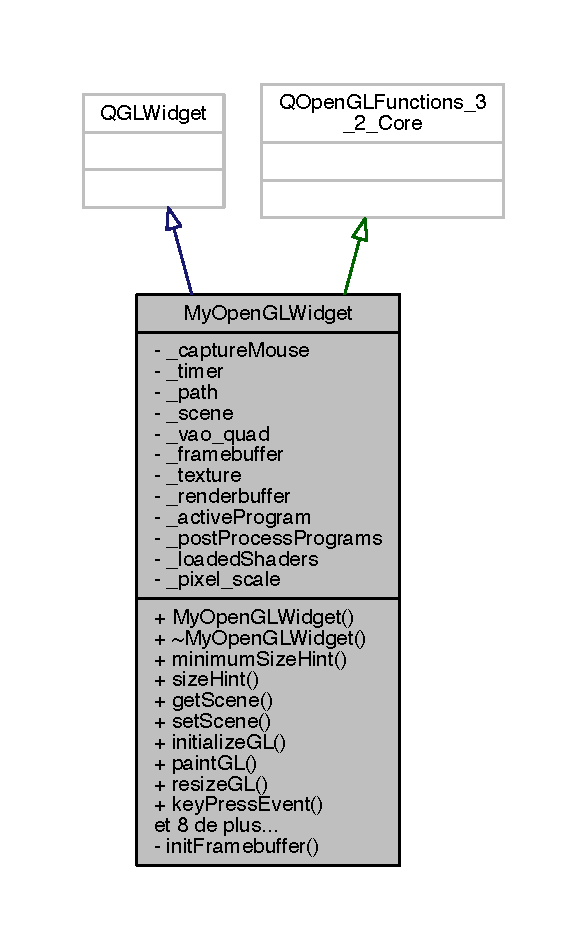
\includegraphics[width=282pt]{class_my_open_g_l_widget__inherit__graph}
\end{center}
\end{figure}


Graphe de collaboration de My\+Open\+G\+L\+Widget\+:
\nopagebreak
\begin{figure}[H]
\begin{center}
\leavevmode
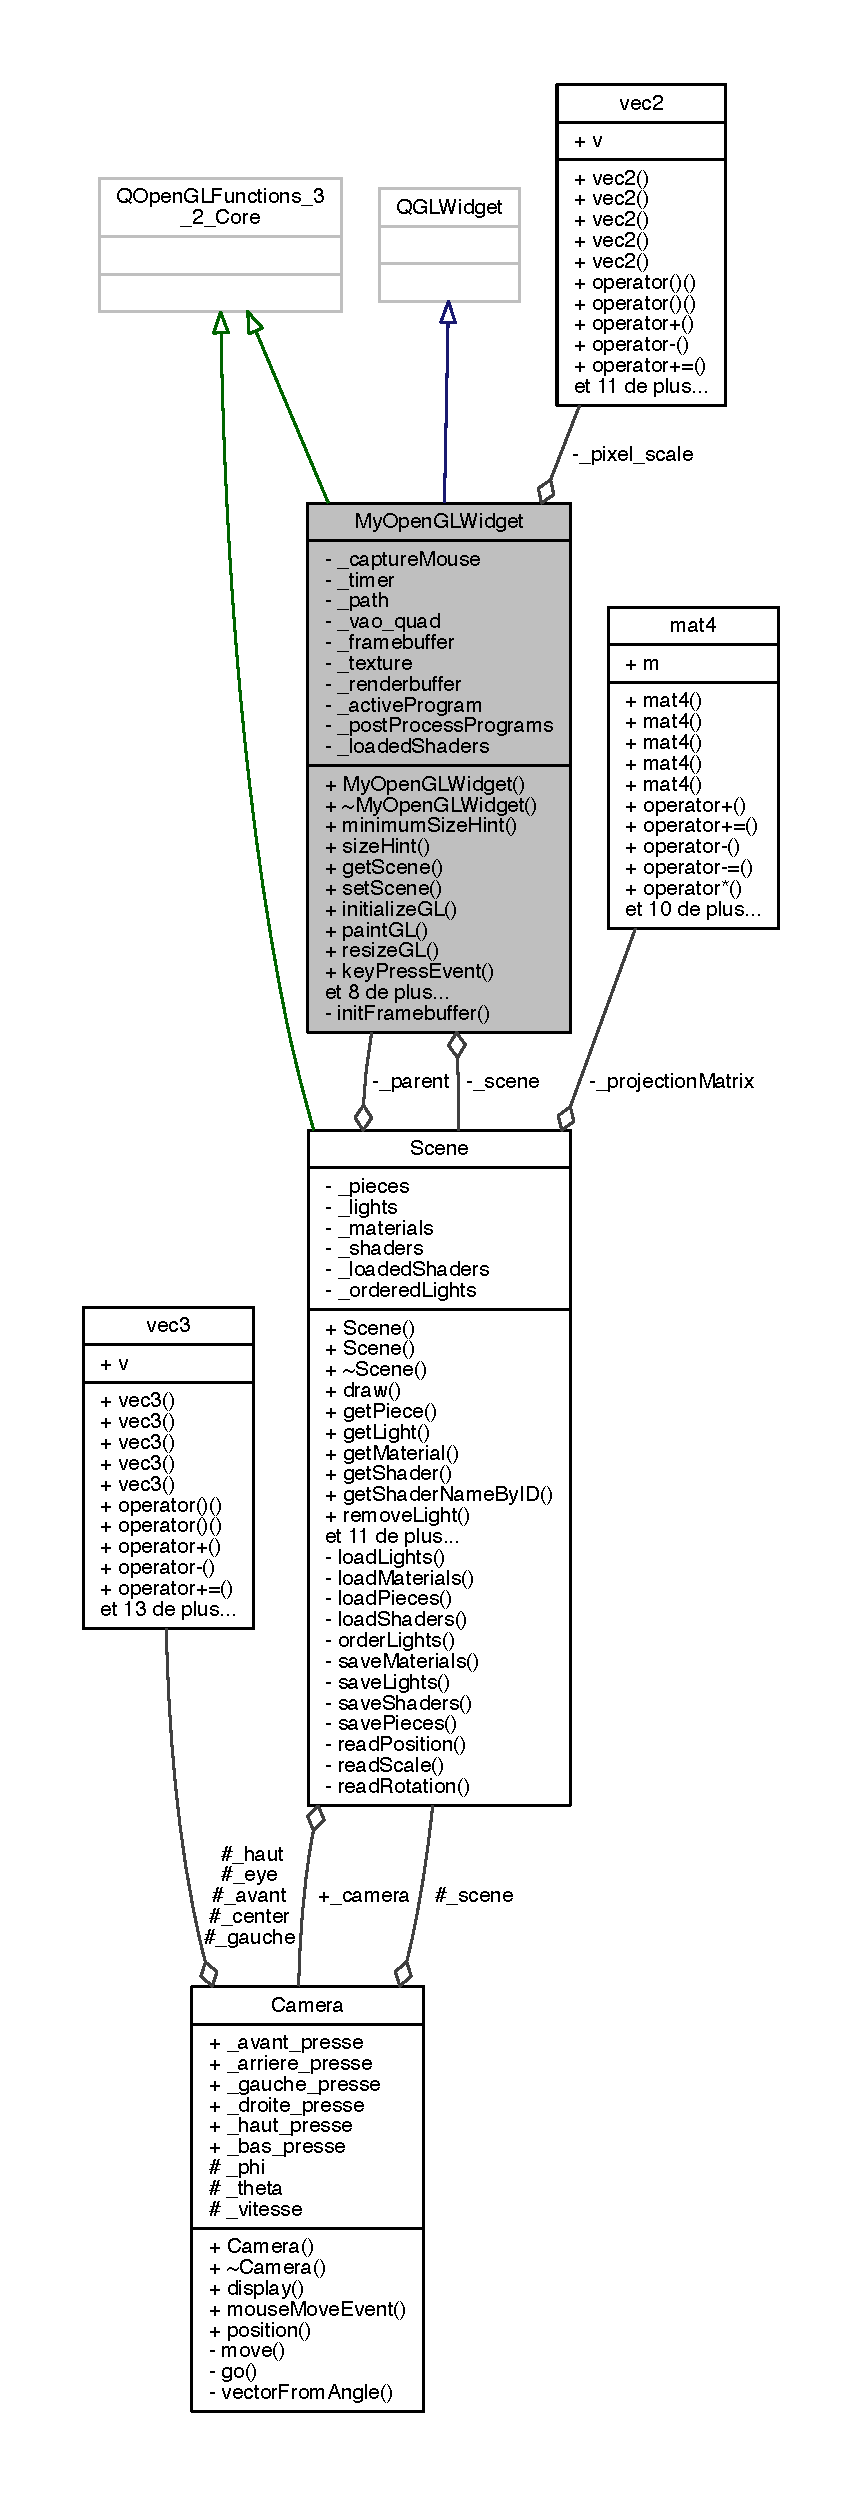
\includegraphics[height=550pt]{class_my_open_g_l_widget__coll__graph}
\end{center}
\end{figure}
\subsection*{Fonctions membres publiques}
\begin{DoxyCompactItemize}
\item 
\hyperlink{class_my_open_g_l_widget_a78f2284f348e8b482875ccdfbf704b34}{My\+Open\+G\+L\+Widget} (const Q\+G\+L\+Format \&format, Q\+Widget $\ast$parent=0, const Q\+String \&path=\char`\"{}\char`\"{}, const Q\+G\+L\+Widget $\ast$share\+Widget=0, Qt\+::\+Window\+Flags f=0)
\item 
\hyperlink{class_my_open_g_l_widget_aa9bdb4eb867d9e0bbfab210732fa5883}{$\sim$\+My\+Open\+G\+L\+Widget} ()
\item 
Q\+Size \hyperlink{class_my_open_g_l_widget_a4a037578f8e21a015e7b2915992fbe5d}{minimum\+Size\+Hint} () const 
\item 
Q\+Size \hyperlink{class_my_open_g_l_widget_abacca5d710f6a81b5edfd164f0148ed6}{size\+Hint} () const 
\item 
\hyperlink{class_scene}{Scene} $\ast$ \hyperlink{class_my_open_g_l_widget_ab25f238721b8e1cba36c2a0350ac57ba}{get\+Scene} ()
\item 
void \hyperlink{class_my_open_g_l_widget_aaac5737e9ce05a94006aa92afed5d403}{set\+Scene} (\hyperlink{class_scene}{Scene} $\ast$scene)
\item 
virtual void \hyperlink{class_my_open_g_l_widget_a98597f5669cec1c90f36c1d38569afc5}{initialize\+G\+L} ()
\item 
virtual void \hyperlink{class_my_open_g_l_widget_af7babfe769e968c317e646c4387b357d}{paint\+G\+L} ()
\item 
virtual void \hyperlink{class_my_open_g_l_widget_a51847d078dbd11fb99335abbc5eaf4fc}{resize\+G\+L} (int width, int height)
\item 
virtual void \hyperlink{class_my_open_g_l_widget_a87a479700547c066721b4b3532b040a2}{key\+Press\+Event} (Q\+Key\+Event $\ast$event)
\item 
virtual void \hyperlink{class_my_open_g_l_widget_a57e054ac1c21ed8585ca57b151ec6b38}{key\+Release\+Event} (Q\+Key\+Event $\ast$event)
\item 
virtual void \hyperlink{class_my_open_g_l_widget_a27abe02c04240317cf42c1cec1ac7e25}{mouse\+Move\+Event} (Q\+Mouse\+Event $\ast$event)
\item 
virtual void \hyperlink{class_my_open_g_l_widget_a6a2e229f91bb75775bb539c85bb696ef}{mouse\+Press\+Event} (Q\+Mouse\+Event $\ast$event)
\item 
void \hyperlink{class_my_open_g_l_widget_a87b9f933f545bf6f257820395771cc8b}{use\+Shader} (const Q\+String \&name)
\item 
void \hyperlink{class_my_open_g_l_widget_a1426e6f24592838e16c22a92870cf5f4}{add\+Shader} (const Q\+String \&name, const Q\+String \&vertex, const Q\+String \&fragment)
\item 
Q\+String\+List \hyperlink{class_my_open_g_l_widget_a99929e3c743d4f5793ef0e09ab61f2b2}{get\+Shader\+Names} ()
\item 
void \hyperlink{class_my_open_g_l_widget_af7899fd91898c1ed5dc228d7d6de658e}{load\+Shaders} (const Q\+Dom\+Element \&post\+Process)
\item 
void \hyperlink{class_my_open_g_l_widget_a177cfabda79d05c834b4f1a3f370a620}{save\+Shaders} (Q\+Dom\+Element \&root, Q\+Dom\+Document \&doc) const 
\end{DoxyCompactItemize}
\subsection*{Fonctions membres privées}
\begin{DoxyCompactItemize}
\item 
void \hyperlink{class_my_open_g_l_widget_ae2bcca23e0802d6f5ebf2ee3e6ed6e7a}{init\+Framebuffer} (int width, int height)
\end{DoxyCompactItemize}
\subsection*{Attributs privés}
\begin{DoxyCompactItemize}
\item 
bool \hyperlink{class_my_open_g_l_widget_af001d889fec5469aa3e67c11ae48b29d}{\+\_\+capture\+Mouse}
\item 
Q\+Timer $\ast$ \hyperlink{class_my_open_g_l_widget_aa6ba509f0ef6e8c2d266b83e1d380eb8}{\+\_\+timer}
\item 
Q\+String \hyperlink{class_my_open_g_l_widget_a7b3d69ddf0b3509a196edbfeb78407c6}{\+\_\+path}
\item 
\hyperlink{class_scene}{Scene} $\ast$ \hyperlink{class_my_open_g_l_widget_a26a1f259357dd7c8822d715d81591395}{\+\_\+scene}
\item 
G\+Luint \hyperlink{class_my_open_g_l_widget_a63a814817d1af6ea49036edac108183b}{\+\_\+vao\+\_\+quad}
\item 
G\+Luint \hyperlink{class_my_open_g_l_widget_ab39ecf367a98c1bd5e1dbeeb8b44a255}{\+\_\+framebuffer}
\item 
G\+Luint \hyperlink{class_my_open_g_l_widget_a18d7f106f5e12568f5db59d8c4a71706}{\+\_\+texture}
\item 
G\+Luint \hyperlink{class_my_open_g_l_widget_a8385a49fb5113010acc3ddd67080ed1a}{\+\_\+renderbuffer}
\item 
Q\+Open\+G\+L\+Shader\+Program $\ast$ \hyperlink{class_my_open_g_l_widget_a24571f61604a92b622b49609bc0f3f5b}{\+\_\+active\+Program}
\item 
Q\+Map$<$ Q\+String, \\*
Q\+Open\+G\+L\+Shader\+Program $\ast$ $>$ \hyperlink{class_my_open_g_l_widget_afde13326f4f01ede3cac0ee4f389a594}{\+\_\+post\+Process\+Programs}
\item 
Q\+Map$<$ Q\+String, Q\+Open\+G\+L\+Shader $\ast$ $>$ \hyperlink{class_my_open_g_l_widget_ab02762bc0b4cb541f7ad42fdbd7a73f7}{\+\_\+loaded\+Shaders}
\item 
\hyperlink{structvec2}{vec2} \hyperlink{class_my_open_g_l_widget_a543e9cc55491a8e07a7bb5eb54633351}{\+\_\+pixel\+\_\+scale}
\end{DoxyCompactItemize}


\subsection{Documentation des constructeurs et destructeur}
\hypertarget{class_my_open_g_l_widget_a78f2284f348e8b482875ccdfbf704b34}{\index{My\+Open\+G\+L\+Widget@{My\+Open\+G\+L\+Widget}!My\+Open\+G\+L\+Widget@{My\+Open\+G\+L\+Widget}}
\index{My\+Open\+G\+L\+Widget@{My\+Open\+G\+L\+Widget}!My\+Open\+G\+L\+Widget@{My\+Open\+G\+L\+Widget}}
\subsubsection[{My\+Open\+G\+L\+Widget}]{\setlength{\rightskip}{0pt plus 5cm}My\+Open\+G\+L\+Widget\+::\+My\+Open\+G\+L\+Widget (
\begin{DoxyParamCaption}
\item[{const Q\+G\+L\+Format \&}]{format, }
\item[{Q\+Widget $\ast$}]{parent = {\ttfamily 0}, }
\item[{const Q\+String \&}]{path = {\ttfamily \char`\"{}\char`\"{}}, }
\item[{const Q\+G\+L\+Widget $\ast$}]{share\+Widget = {\ttfamily 0}, }
\item[{Qt\+::\+Window\+Flags}]{f = {\ttfamily 0}}
\end{DoxyParamCaption}
)}}\label{class_my_open_g_l_widget_a78f2284f348e8b482875ccdfbf704b34}
\hypertarget{class_my_open_g_l_widget_aa9bdb4eb867d9e0bbfab210732fa5883}{\index{My\+Open\+G\+L\+Widget@{My\+Open\+G\+L\+Widget}!````~My\+Open\+G\+L\+Widget@{$\sim$\+My\+Open\+G\+L\+Widget}}
\index{````~My\+Open\+G\+L\+Widget@{$\sim$\+My\+Open\+G\+L\+Widget}!My\+Open\+G\+L\+Widget@{My\+Open\+G\+L\+Widget}}
\subsubsection[{$\sim$\+My\+Open\+G\+L\+Widget}]{\setlength{\rightskip}{0pt plus 5cm}My\+Open\+G\+L\+Widget\+::$\sim$\+My\+Open\+G\+L\+Widget (
\begin{DoxyParamCaption}
{}
\end{DoxyParamCaption}
)}}\label{class_my_open_g_l_widget_aa9bdb4eb867d9e0bbfab210732fa5883}


\subsection{Documentation des fonctions membres}
\hypertarget{class_my_open_g_l_widget_a1426e6f24592838e16c22a92870cf5f4}{\index{My\+Open\+G\+L\+Widget@{My\+Open\+G\+L\+Widget}!add\+Shader@{add\+Shader}}
\index{add\+Shader@{add\+Shader}!My\+Open\+G\+L\+Widget@{My\+Open\+G\+L\+Widget}}
\subsubsection[{add\+Shader}]{\setlength{\rightskip}{0pt plus 5cm}void My\+Open\+G\+L\+Widget\+::add\+Shader (
\begin{DoxyParamCaption}
\item[{const Q\+String \&}]{name, }
\item[{const Q\+String \&}]{vertex, }
\item[{const Q\+String \&}]{fragment}
\end{DoxyParamCaption}
)}}\label{class_my_open_g_l_widget_a1426e6f24592838e16c22a92870cf5f4}


Voici le graphe des appelants de cette fonction \+:
\nopagebreak
\begin{figure}[H]
\begin{center}
\leavevmode
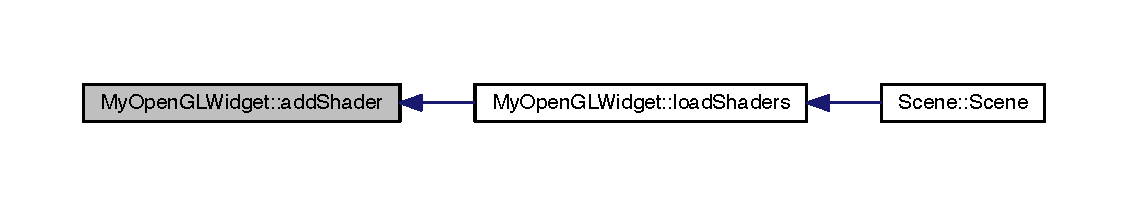
\includegraphics[width=350pt]{class_my_open_g_l_widget_a1426e6f24592838e16c22a92870cf5f4_icgraph}
\end{center}
\end{figure}


\hypertarget{class_my_open_g_l_widget_ab25f238721b8e1cba36c2a0350ac57ba}{\index{My\+Open\+G\+L\+Widget@{My\+Open\+G\+L\+Widget}!get\+Scene@{get\+Scene}}
\index{get\+Scene@{get\+Scene}!My\+Open\+G\+L\+Widget@{My\+Open\+G\+L\+Widget}}
\subsubsection[{get\+Scene}]{\setlength{\rightskip}{0pt plus 5cm}{\bf Scene} $\ast$ My\+Open\+G\+L\+Widget\+::get\+Scene (
\begin{DoxyParamCaption}
{}
\end{DoxyParamCaption}
)}}\label{class_my_open_g_l_widget_ab25f238721b8e1cba36c2a0350ac57ba}


Voici le graphe des appelants de cette fonction \+:
\nopagebreak
\begin{figure}[H]
\begin{center}
\leavevmode
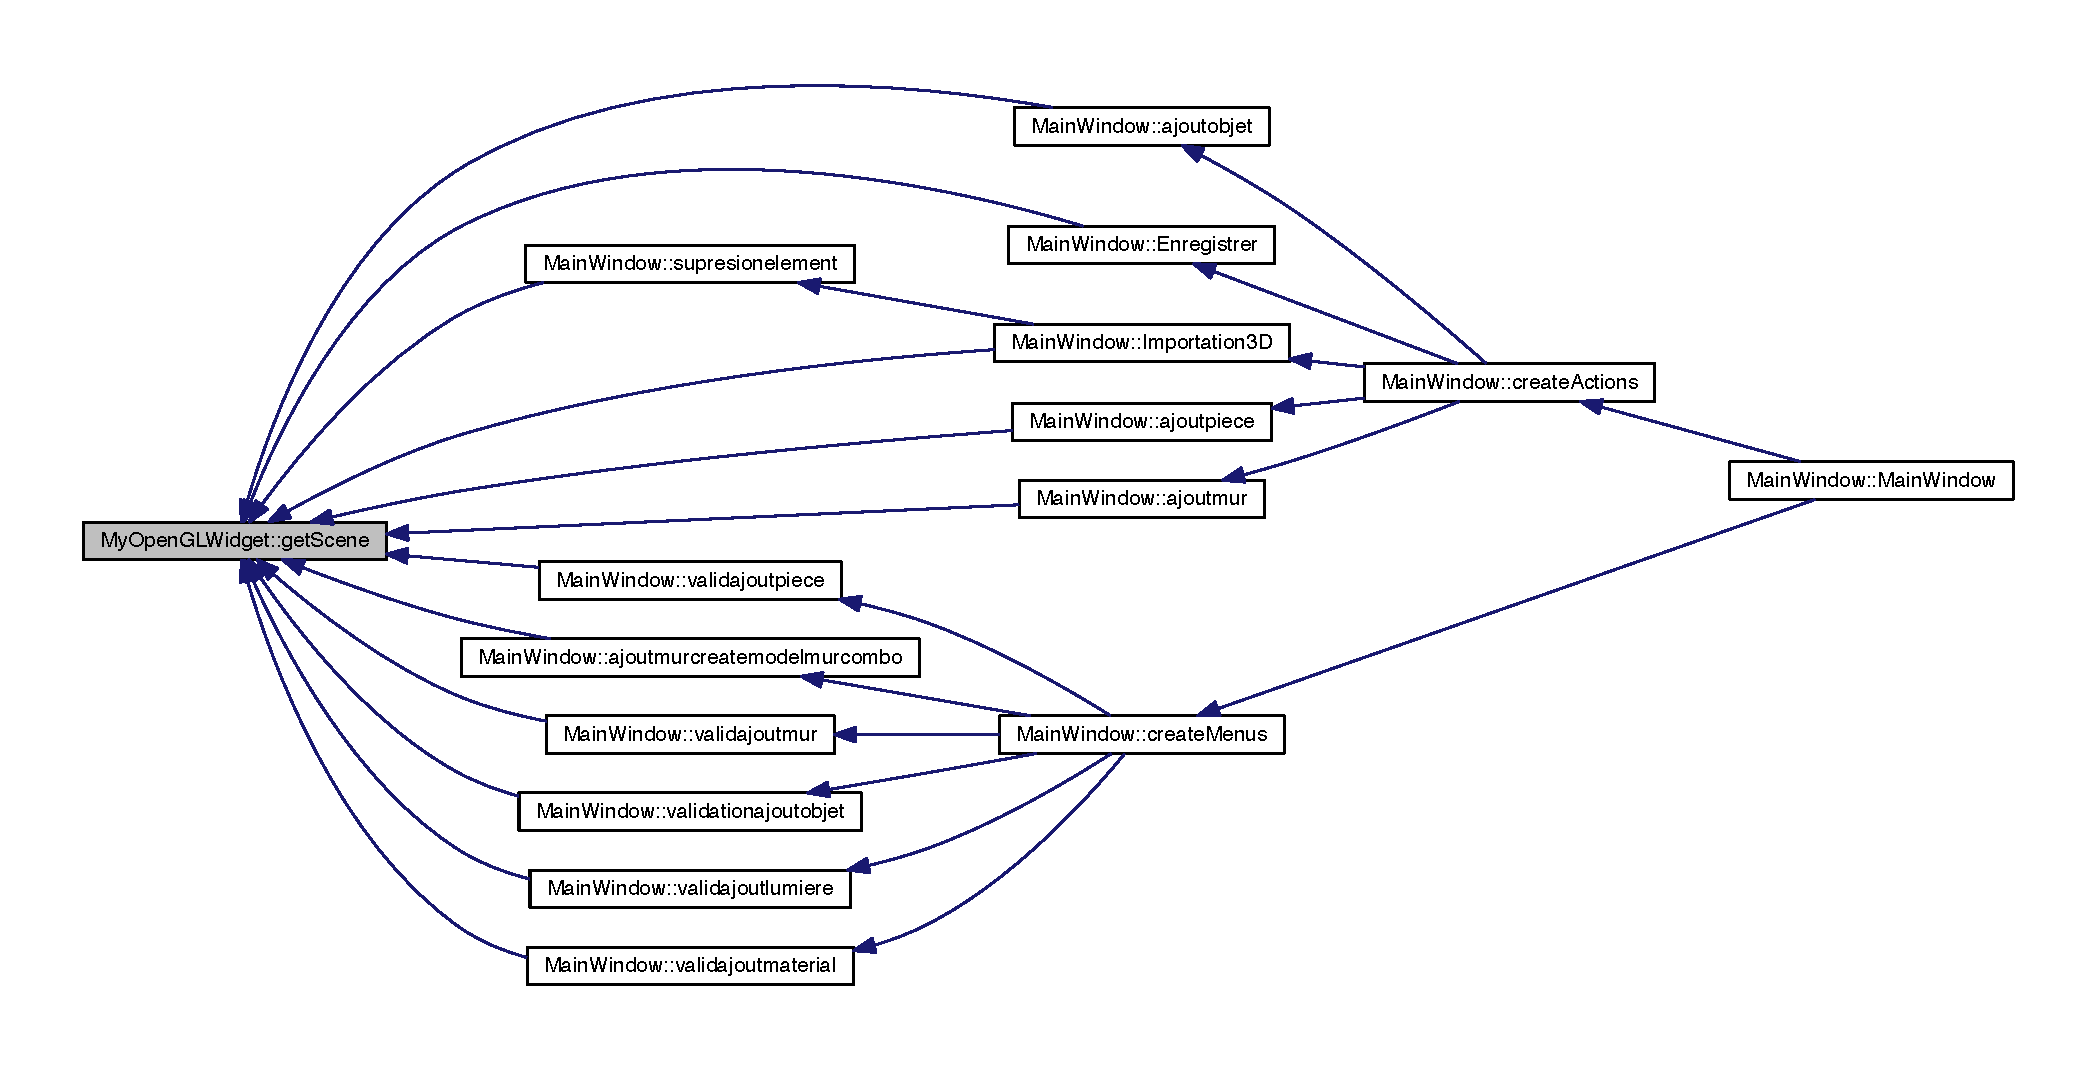
\includegraphics[width=350pt]{class_my_open_g_l_widget_ab25f238721b8e1cba36c2a0350ac57ba_icgraph}
\end{center}
\end{figure}


\hypertarget{class_my_open_g_l_widget_a99929e3c743d4f5793ef0e09ab61f2b2}{\index{My\+Open\+G\+L\+Widget@{My\+Open\+G\+L\+Widget}!get\+Shader\+Names@{get\+Shader\+Names}}
\index{get\+Shader\+Names@{get\+Shader\+Names}!My\+Open\+G\+L\+Widget@{My\+Open\+G\+L\+Widget}}
\subsubsection[{get\+Shader\+Names}]{\setlength{\rightskip}{0pt plus 5cm}Q\+String\+List My\+Open\+G\+L\+Widget\+::get\+Shader\+Names (
\begin{DoxyParamCaption}
{}
\end{DoxyParamCaption}
)}}\label{class_my_open_g_l_widget_a99929e3c743d4f5793ef0e09ab61f2b2}


Voici le graphe des appelants de cette fonction \+:
\nopagebreak
\begin{figure}[H]
\begin{center}
\leavevmode
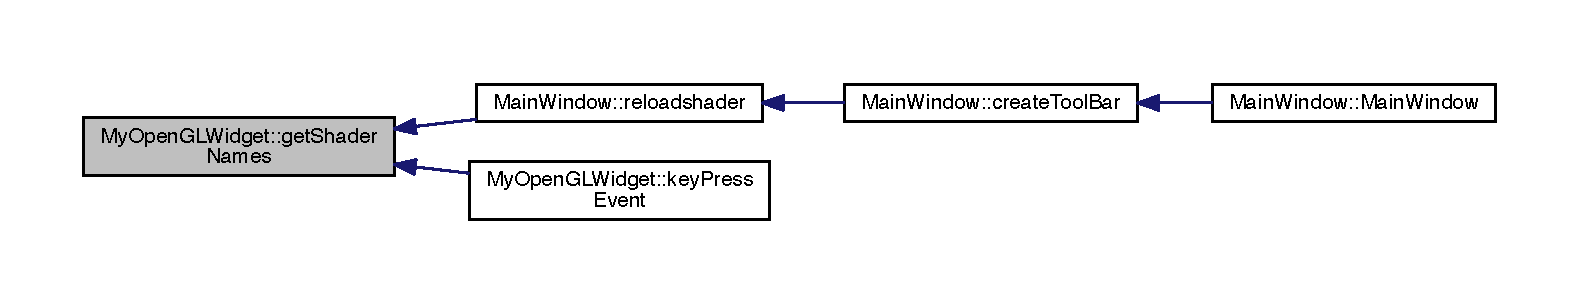
\includegraphics[width=350pt]{class_my_open_g_l_widget_a99929e3c743d4f5793ef0e09ab61f2b2_icgraph}
\end{center}
\end{figure}


\hypertarget{class_my_open_g_l_widget_ae2bcca23e0802d6f5ebf2ee3e6ed6e7a}{\index{My\+Open\+G\+L\+Widget@{My\+Open\+G\+L\+Widget}!init\+Framebuffer@{init\+Framebuffer}}
\index{init\+Framebuffer@{init\+Framebuffer}!My\+Open\+G\+L\+Widget@{My\+Open\+G\+L\+Widget}}
\subsubsection[{init\+Framebuffer}]{\setlength{\rightskip}{0pt plus 5cm}void My\+Open\+G\+L\+Widget\+::init\+Framebuffer (
\begin{DoxyParamCaption}
\item[{int}]{width, }
\item[{int}]{height}
\end{DoxyParamCaption}
)\hspace{0.3cm}{\ttfamily [private]}}}\label{class_my_open_g_l_widget_ae2bcca23e0802d6f5ebf2ee3e6ed6e7a}


Voici le graphe des appelants de cette fonction \+:
\nopagebreak
\begin{figure}[H]
\begin{center}
\leavevmode
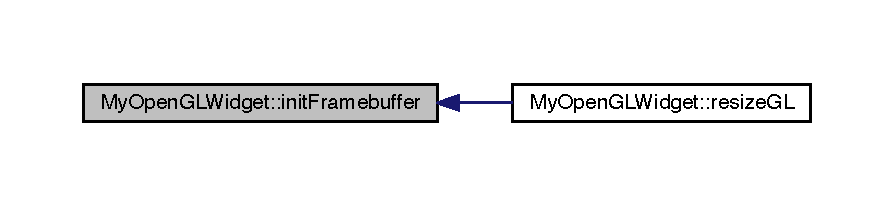
\includegraphics[width=350pt]{class_my_open_g_l_widget_ae2bcca23e0802d6f5ebf2ee3e6ed6e7a_icgraph}
\end{center}
\end{figure}


\hypertarget{class_my_open_g_l_widget_a98597f5669cec1c90f36c1d38569afc5}{\index{My\+Open\+G\+L\+Widget@{My\+Open\+G\+L\+Widget}!initialize\+G\+L@{initialize\+G\+L}}
\index{initialize\+G\+L@{initialize\+G\+L}!My\+Open\+G\+L\+Widget@{My\+Open\+G\+L\+Widget}}
\subsubsection[{initialize\+G\+L}]{\setlength{\rightskip}{0pt plus 5cm}void My\+Open\+G\+L\+Widget\+::initialize\+G\+L (
\begin{DoxyParamCaption}
{}
\end{DoxyParamCaption}
)\hspace{0.3cm}{\ttfamily [virtual]}}}\label{class_my_open_g_l_widget_a98597f5669cec1c90f36c1d38569afc5}
\hypertarget{class_my_open_g_l_widget_a87a479700547c066721b4b3532b040a2}{\index{My\+Open\+G\+L\+Widget@{My\+Open\+G\+L\+Widget}!key\+Press\+Event@{key\+Press\+Event}}
\index{key\+Press\+Event@{key\+Press\+Event}!My\+Open\+G\+L\+Widget@{My\+Open\+G\+L\+Widget}}
\subsubsection[{key\+Press\+Event}]{\setlength{\rightskip}{0pt plus 5cm}void My\+Open\+G\+L\+Widget\+::key\+Press\+Event (
\begin{DoxyParamCaption}
\item[{Q\+Key\+Event $\ast$}]{event}
\end{DoxyParamCaption}
)\hspace{0.3cm}{\ttfamily [virtual]}}}\label{class_my_open_g_l_widget_a87a479700547c066721b4b3532b040a2}


Voici le graphe d'appel pour cette fonction \+:
\nopagebreak
\begin{figure}[H]
\begin{center}
\leavevmode
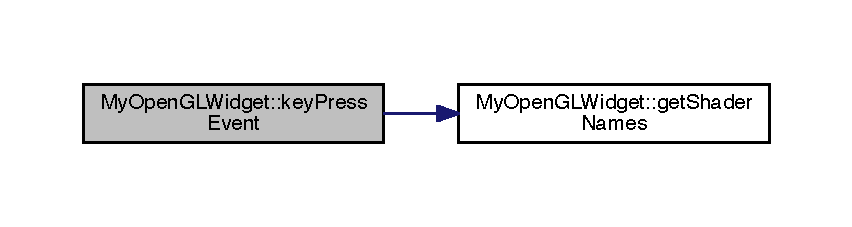
\includegraphics[width=350pt]{class_my_open_g_l_widget_a87a479700547c066721b4b3532b040a2_cgraph}
\end{center}
\end{figure}


\hypertarget{class_my_open_g_l_widget_a57e054ac1c21ed8585ca57b151ec6b38}{\index{My\+Open\+G\+L\+Widget@{My\+Open\+G\+L\+Widget}!key\+Release\+Event@{key\+Release\+Event}}
\index{key\+Release\+Event@{key\+Release\+Event}!My\+Open\+G\+L\+Widget@{My\+Open\+G\+L\+Widget}}
\subsubsection[{key\+Release\+Event}]{\setlength{\rightskip}{0pt plus 5cm}void My\+Open\+G\+L\+Widget\+::key\+Release\+Event (
\begin{DoxyParamCaption}
\item[{Q\+Key\+Event $\ast$}]{event}
\end{DoxyParamCaption}
)\hspace{0.3cm}{\ttfamily [virtual]}}}\label{class_my_open_g_l_widget_a57e054ac1c21ed8585ca57b151ec6b38}
\hypertarget{class_my_open_g_l_widget_af7899fd91898c1ed5dc228d7d6de658e}{\index{My\+Open\+G\+L\+Widget@{My\+Open\+G\+L\+Widget}!load\+Shaders@{load\+Shaders}}
\index{load\+Shaders@{load\+Shaders}!My\+Open\+G\+L\+Widget@{My\+Open\+G\+L\+Widget}}
\subsubsection[{load\+Shaders}]{\setlength{\rightskip}{0pt plus 5cm}void My\+Open\+G\+L\+Widget\+::load\+Shaders (
\begin{DoxyParamCaption}
\item[{const Q\+Dom\+Element \&}]{post\+Process}
\end{DoxyParamCaption}
)}}\label{class_my_open_g_l_widget_af7899fd91898c1ed5dc228d7d6de658e}


Voici le graphe d'appel pour cette fonction \+:
\nopagebreak
\begin{figure}[H]
\begin{center}
\leavevmode
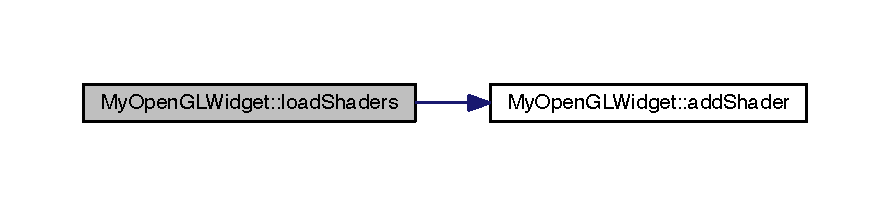
\includegraphics[width=350pt]{class_my_open_g_l_widget_af7899fd91898c1ed5dc228d7d6de658e_cgraph}
\end{center}
\end{figure}




Voici le graphe des appelants de cette fonction \+:
\nopagebreak
\begin{figure}[H]
\begin{center}
\leavevmode
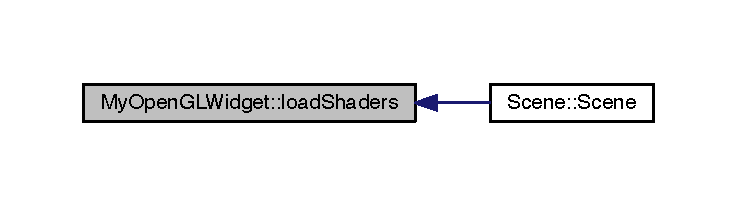
\includegraphics[width=350pt]{class_my_open_g_l_widget_af7899fd91898c1ed5dc228d7d6de658e_icgraph}
\end{center}
\end{figure}


\hypertarget{class_my_open_g_l_widget_a4a037578f8e21a015e7b2915992fbe5d}{\index{My\+Open\+G\+L\+Widget@{My\+Open\+G\+L\+Widget}!minimum\+Size\+Hint@{minimum\+Size\+Hint}}
\index{minimum\+Size\+Hint@{minimum\+Size\+Hint}!My\+Open\+G\+L\+Widget@{My\+Open\+G\+L\+Widget}}
\subsubsection[{minimum\+Size\+Hint}]{\setlength{\rightskip}{0pt plus 5cm}Q\+Size My\+Open\+G\+L\+Widget\+::minimum\+Size\+Hint (
\begin{DoxyParamCaption}
{}
\end{DoxyParamCaption}
) const}}\label{class_my_open_g_l_widget_a4a037578f8e21a015e7b2915992fbe5d}
\hypertarget{class_my_open_g_l_widget_a27abe02c04240317cf42c1cec1ac7e25}{\index{My\+Open\+G\+L\+Widget@{My\+Open\+G\+L\+Widget}!mouse\+Move\+Event@{mouse\+Move\+Event}}
\index{mouse\+Move\+Event@{mouse\+Move\+Event}!My\+Open\+G\+L\+Widget@{My\+Open\+G\+L\+Widget}}
\subsubsection[{mouse\+Move\+Event}]{\setlength{\rightskip}{0pt plus 5cm}void My\+Open\+G\+L\+Widget\+::mouse\+Move\+Event (
\begin{DoxyParamCaption}
\item[{Q\+Mouse\+Event $\ast$}]{event}
\end{DoxyParamCaption}
)\hspace{0.3cm}{\ttfamily [virtual]}}}\label{class_my_open_g_l_widget_a27abe02c04240317cf42c1cec1ac7e25}


Voici le graphe d'appel pour cette fonction \+:
\nopagebreak
\begin{figure}[H]
\begin{center}
\leavevmode
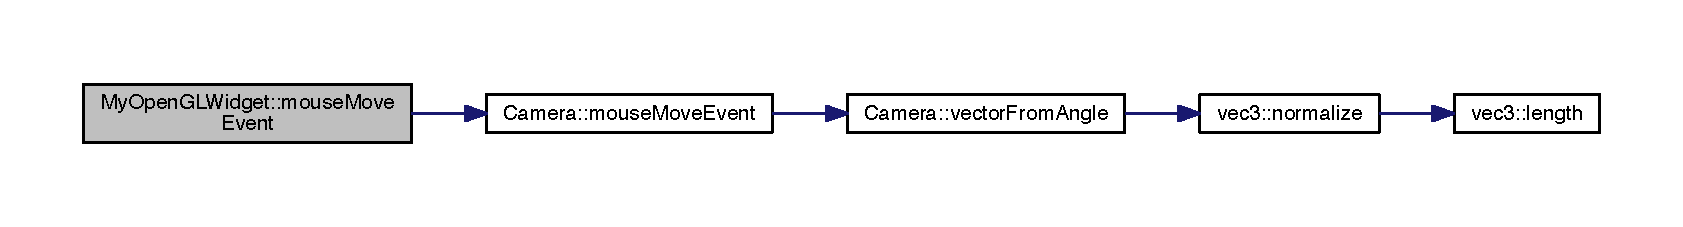
\includegraphics[width=350pt]{class_my_open_g_l_widget_a27abe02c04240317cf42c1cec1ac7e25_cgraph}
\end{center}
\end{figure}


\hypertarget{class_my_open_g_l_widget_a6a2e229f91bb75775bb539c85bb696ef}{\index{My\+Open\+G\+L\+Widget@{My\+Open\+G\+L\+Widget}!mouse\+Press\+Event@{mouse\+Press\+Event}}
\index{mouse\+Press\+Event@{mouse\+Press\+Event}!My\+Open\+G\+L\+Widget@{My\+Open\+G\+L\+Widget}}
\subsubsection[{mouse\+Press\+Event}]{\setlength{\rightskip}{0pt plus 5cm}void My\+Open\+G\+L\+Widget\+::mouse\+Press\+Event (
\begin{DoxyParamCaption}
\item[{Q\+Mouse\+Event $\ast$}]{event}
\end{DoxyParamCaption}
)\hspace{0.3cm}{\ttfamily [virtual]}}}\label{class_my_open_g_l_widget_a6a2e229f91bb75775bb539c85bb696ef}
\hypertarget{class_my_open_g_l_widget_af7babfe769e968c317e646c4387b357d}{\index{My\+Open\+G\+L\+Widget@{My\+Open\+G\+L\+Widget}!paint\+G\+L@{paint\+G\+L}}
\index{paint\+G\+L@{paint\+G\+L}!My\+Open\+G\+L\+Widget@{My\+Open\+G\+L\+Widget}}
\subsubsection[{paint\+G\+L}]{\setlength{\rightskip}{0pt plus 5cm}void My\+Open\+G\+L\+Widget\+::paint\+G\+L (
\begin{DoxyParamCaption}
{}
\end{DoxyParamCaption}
)\hspace{0.3cm}{\ttfamily [virtual]}}}\label{class_my_open_g_l_widget_af7babfe769e968c317e646c4387b357d}


Voici le graphe d'appel pour cette fonction \+:
\nopagebreak
\begin{figure}[H]
\begin{center}
\leavevmode
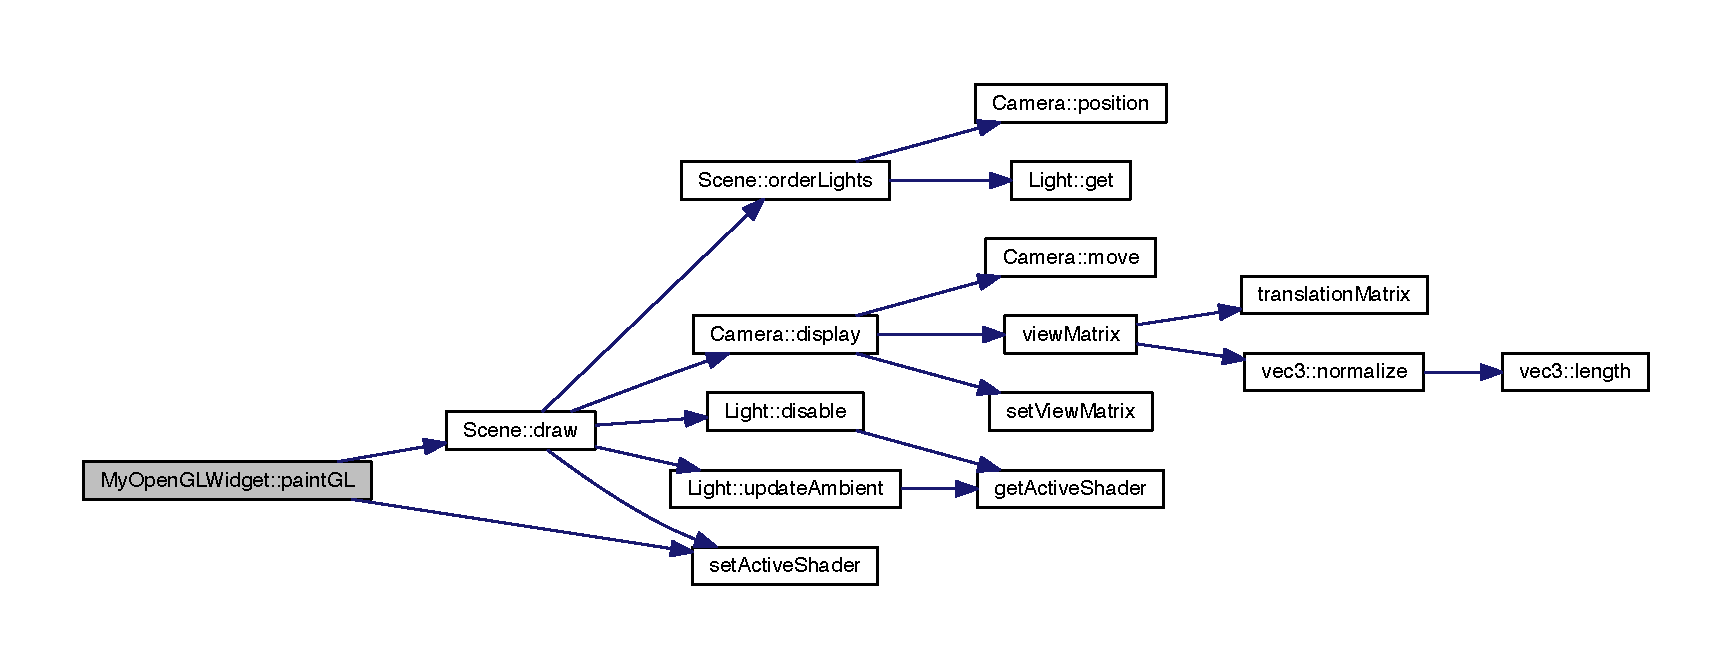
\includegraphics[width=350pt]{class_my_open_g_l_widget_af7babfe769e968c317e646c4387b357d_cgraph}
\end{center}
\end{figure}


\hypertarget{class_my_open_g_l_widget_a51847d078dbd11fb99335abbc5eaf4fc}{\index{My\+Open\+G\+L\+Widget@{My\+Open\+G\+L\+Widget}!resize\+G\+L@{resize\+G\+L}}
\index{resize\+G\+L@{resize\+G\+L}!My\+Open\+G\+L\+Widget@{My\+Open\+G\+L\+Widget}}
\subsubsection[{resize\+G\+L}]{\setlength{\rightskip}{0pt plus 5cm}void My\+Open\+G\+L\+Widget\+::resize\+G\+L (
\begin{DoxyParamCaption}
\item[{int}]{width, }
\item[{int}]{height}
\end{DoxyParamCaption}
)\hspace{0.3cm}{\ttfamily [virtual]}}}\label{class_my_open_g_l_widget_a51847d078dbd11fb99335abbc5eaf4fc}


Voici le graphe d'appel pour cette fonction \+:
\nopagebreak
\begin{figure}[H]
\begin{center}
\leavevmode
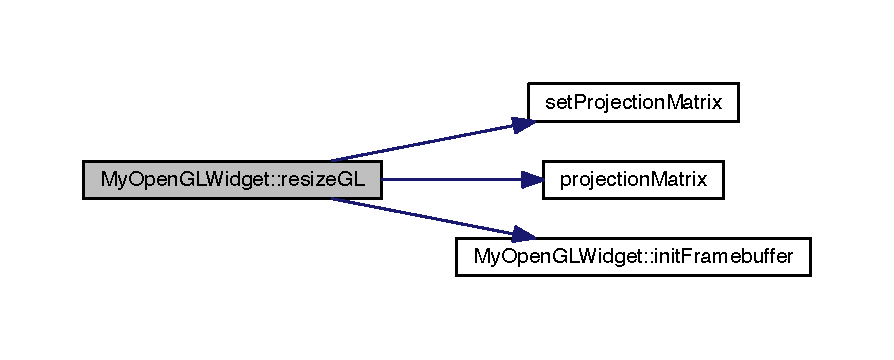
\includegraphics[width=350pt]{class_my_open_g_l_widget_a51847d078dbd11fb99335abbc5eaf4fc_cgraph}
\end{center}
\end{figure}


\hypertarget{class_my_open_g_l_widget_a177cfabda79d05c834b4f1a3f370a620}{\index{My\+Open\+G\+L\+Widget@{My\+Open\+G\+L\+Widget}!save\+Shaders@{save\+Shaders}}
\index{save\+Shaders@{save\+Shaders}!My\+Open\+G\+L\+Widget@{My\+Open\+G\+L\+Widget}}
\subsubsection[{save\+Shaders}]{\setlength{\rightskip}{0pt plus 5cm}void My\+Open\+G\+L\+Widget\+::save\+Shaders (
\begin{DoxyParamCaption}
\item[{Q\+Dom\+Element \&}]{root, }
\item[{Q\+Dom\+Document \&}]{doc}
\end{DoxyParamCaption}
) const}}\label{class_my_open_g_l_widget_a177cfabda79d05c834b4f1a3f370a620}


Voici le graphe des appelants de cette fonction \+:
\nopagebreak
\begin{figure}[H]
\begin{center}
\leavevmode
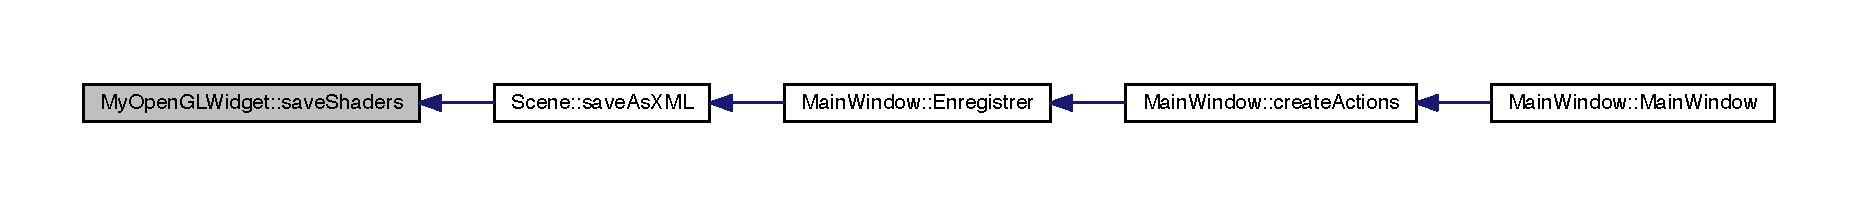
\includegraphics[width=350pt]{class_my_open_g_l_widget_a177cfabda79d05c834b4f1a3f370a620_icgraph}
\end{center}
\end{figure}


\hypertarget{class_my_open_g_l_widget_aaac5737e9ce05a94006aa92afed5d403}{\index{My\+Open\+G\+L\+Widget@{My\+Open\+G\+L\+Widget}!set\+Scene@{set\+Scene}}
\index{set\+Scene@{set\+Scene}!My\+Open\+G\+L\+Widget@{My\+Open\+G\+L\+Widget}}
\subsubsection[{set\+Scene}]{\setlength{\rightskip}{0pt plus 5cm}void My\+Open\+G\+L\+Widget\+::set\+Scene (
\begin{DoxyParamCaption}
\item[{{\bf Scene} $\ast$}]{scene}
\end{DoxyParamCaption}
)}}\label{class_my_open_g_l_widget_aaac5737e9ce05a94006aa92afed5d403}
\hypertarget{class_my_open_g_l_widget_abacca5d710f6a81b5edfd164f0148ed6}{\index{My\+Open\+G\+L\+Widget@{My\+Open\+G\+L\+Widget}!size\+Hint@{size\+Hint}}
\index{size\+Hint@{size\+Hint}!My\+Open\+G\+L\+Widget@{My\+Open\+G\+L\+Widget}}
\subsubsection[{size\+Hint}]{\setlength{\rightskip}{0pt plus 5cm}Q\+Size My\+Open\+G\+L\+Widget\+::size\+Hint (
\begin{DoxyParamCaption}
{}
\end{DoxyParamCaption}
) const}}\label{class_my_open_g_l_widget_abacca5d710f6a81b5edfd164f0148ed6}
\hypertarget{class_my_open_g_l_widget_a87b9f933f545bf6f257820395771cc8b}{\index{My\+Open\+G\+L\+Widget@{My\+Open\+G\+L\+Widget}!use\+Shader@{use\+Shader}}
\index{use\+Shader@{use\+Shader}!My\+Open\+G\+L\+Widget@{My\+Open\+G\+L\+Widget}}
\subsubsection[{use\+Shader}]{\setlength{\rightskip}{0pt plus 5cm}void My\+Open\+G\+L\+Widget\+::use\+Shader (
\begin{DoxyParamCaption}
\item[{const Q\+String \&}]{name}
\end{DoxyParamCaption}
)}}\label{class_my_open_g_l_widget_a87b9f933f545bf6f257820395771cc8b}


Voici le graphe des appelants de cette fonction \+:
\nopagebreak
\begin{figure}[H]
\begin{center}
\leavevmode
\includegraphics[width=350pt]{class_my_open_g_l_widget_a87b9f933f545bf6f257820395771cc8b_icgraph}
\end{center}
\end{figure}




\subsection{Documentation des données membres}
\hypertarget{class_my_open_g_l_widget_a24571f61604a92b622b49609bc0f3f5b}{\index{My\+Open\+G\+L\+Widget@{My\+Open\+G\+L\+Widget}!\+\_\+active\+Program@{\+\_\+active\+Program}}
\index{\+\_\+active\+Program@{\+\_\+active\+Program}!My\+Open\+G\+L\+Widget@{My\+Open\+G\+L\+Widget}}
\subsubsection[{\+\_\+active\+Program}]{\setlength{\rightskip}{0pt plus 5cm}Q\+Open\+G\+L\+Shader\+Program$\ast$ My\+Open\+G\+L\+Widget\+::\+\_\+active\+Program\hspace{0.3cm}{\ttfamily [private]}}}\label{class_my_open_g_l_widget_a24571f61604a92b622b49609bc0f3f5b}
\hypertarget{class_my_open_g_l_widget_af001d889fec5469aa3e67c11ae48b29d}{\index{My\+Open\+G\+L\+Widget@{My\+Open\+G\+L\+Widget}!\+\_\+capture\+Mouse@{\+\_\+capture\+Mouse}}
\index{\+\_\+capture\+Mouse@{\+\_\+capture\+Mouse}!My\+Open\+G\+L\+Widget@{My\+Open\+G\+L\+Widget}}
\subsubsection[{\+\_\+capture\+Mouse}]{\setlength{\rightskip}{0pt plus 5cm}bool My\+Open\+G\+L\+Widget\+::\+\_\+capture\+Mouse\hspace{0.3cm}{\ttfamily [private]}}}\label{class_my_open_g_l_widget_af001d889fec5469aa3e67c11ae48b29d}
\hypertarget{class_my_open_g_l_widget_ab39ecf367a98c1bd5e1dbeeb8b44a255}{\index{My\+Open\+G\+L\+Widget@{My\+Open\+G\+L\+Widget}!\+\_\+framebuffer@{\+\_\+framebuffer}}
\index{\+\_\+framebuffer@{\+\_\+framebuffer}!My\+Open\+G\+L\+Widget@{My\+Open\+G\+L\+Widget}}
\subsubsection[{\+\_\+framebuffer}]{\setlength{\rightskip}{0pt plus 5cm}G\+Luint My\+Open\+G\+L\+Widget\+::\+\_\+framebuffer\hspace{0.3cm}{\ttfamily [private]}}}\label{class_my_open_g_l_widget_ab39ecf367a98c1bd5e1dbeeb8b44a255}
\hypertarget{class_my_open_g_l_widget_ab02762bc0b4cb541f7ad42fdbd7a73f7}{\index{My\+Open\+G\+L\+Widget@{My\+Open\+G\+L\+Widget}!\+\_\+loaded\+Shaders@{\+\_\+loaded\+Shaders}}
\index{\+\_\+loaded\+Shaders@{\+\_\+loaded\+Shaders}!My\+Open\+G\+L\+Widget@{My\+Open\+G\+L\+Widget}}
\subsubsection[{\+\_\+loaded\+Shaders}]{\setlength{\rightskip}{0pt plus 5cm}Q\+Map$<$Q\+String, Q\+Open\+G\+L\+Shader $\ast$$>$ My\+Open\+G\+L\+Widget\+::\+\_\+loaded\+Shaders\hspace{0.3cm}{\ttfamily [private]}}}\label{class_my_open_g_l_widget_ab02762bc0b4cb541f7ad42fdbd7a73f7}
\hypertarget{class_my_open_g_l_widget_a7b3d69ddf0b3509a196edbfeb78407c6}{\index{My\+Open\+G\+L\+Widget@{My\+Open\+G\+L\+Widget}!\+\_\+path@{\+\_\+path}}
\index{\+\_\+path@{\+\_\+path}!My\+Open\+G\+L\+Widget@{My\+Open\+G\+L\+Widget}}
\subsubsection[{\+\_\+path}]{\setlength{\rightskip}{0pt plus 5cm}Q\+String My\+Open\+G\+L\+Widget\+::\+\_\+path\hspace{0.3cm}{\ttfamily [private]}}}\label{class_my_open_g_l_widget_a7b3d69ddf0b3509a196edbfeb78407c6}
\hypertarget{class_my_open_g_l_widget_a543e9cc55491a8e07a7bb5eb54633351}{\index{My\+Open\+G\+L\+Widget@{My\+Open\+G\+L\+Widget}!\+\_\+pixel\+\_\+scale@{\+\_\+pixel\+\_\+scale}}
\index{\+\_\+pixel\+\_\+scale@{\+\_\+pixel\+\_\+scale}!My\+Open\+G\+L\+Widget@{My\+Open\+G\+L\+Widget}}
\subsubsection[{\+\_\+pixel\+\_\+scale}]{\setlength{\rightskip}{0pt plus 5cm}{\bf vec2} My\+Open\+G\+L\+Widget\+::\+\_\+pixel\+\_\+scale\hspace{0.3cm}{\ttfamily [private]}}}\label{class_my_open_g_l_widget_a543e9cc55491a8e07a7bb5eb54633351}
\hypertarget{class_my_open_g_l_widget_afde13326f4f01ede3cac0ee4f389a594}{\index{My\+Open\+G\+L\+Widget@{My\+Open\+G\+L\+Widget}!\+\_\+post\+Process\+Programs@{\+\_\+post\+Process\+Programs}}
\index{\+\_\+post\+Process\+Programs@{\+\_\+post\+Process\+Programs}!My\+Open\+G\+L\+Widget@{My\+Open\+G\+L\+Widget}}
\subsubsection[{\+\_\+post\+Process\+Programs}]{\setlength{\rightskip}{0pt plus 5cm}Q\+Map$<$Q\+String, Q\+Open\+G\+L\+Shader\+Program $\ast$$>$ My\+Open\+G\+L\+Widget\+::\+\_\+post\+Process\+Programs\hspace{0.3cm}{\ttfamily [private]}}}\label{class_my_open_g_l_widget_afde13326f4f01ede3cac0ee4f389a594}
\hypertarget{class_my_open_g_l_widget_a8385a49fb5113010acc3ddd67080ed1a}{\index{My\+Open\+G\+L\+Widget@{My\+Open\+G\+L\+Widget}!\+\_\+renderbuffer@{\+\_\+renderbuffer}}
\index{\+\_\+renderbuffer@{\+\_\+renderbuffer}!My\+Open\+G\+L\+Widget@{My\+Open\+G\+L\+Widget}}
\subsubsection[{\+\_\+renderbuffer}]{\setlength{\rightskip}{0pt plus 5cm}G\+Luint My\+Open\+G\+L\+Widget\+::\+\_\+renderbuffer\hspace{0.3cm}{\ttfamily [private]}}}\label{class_my_open_g_l_widget_a8385a49fb5113010acc3ddd67080ed1a}
\hypertarget{class_my_open_g_l_widget_a26a1f259357dd7c8822d715d81591395}{\index{My\+Open\+G\+L\+Widget@{My\+Open\+G\+L\+Widget}!\+\_\+scene@{\+\_\+scene}}
\index{\+\_\+scene@{\+\_\+scene}!My\+Open\+G\+L\+Widget@{My\+Open\+G\+L\+Widget}}
\subsubsection[{\+\_\+scene}]{\setlength{\rightskip}{0pt plus 5cm}{\bf Scene}$\ast$ My\+Open\+G\+L\+Widget\+::\+\_\+scene\hspace{0.3cm}{\ttfamily [private]}}}\label{class_my_open_g_l_widget_a26a1f259357dd7c8822d715d81591395}
\hypertarget{class_my_open_g_l_widget_a18d7f106f5e12568f5db59d8c4a71706}{\index{My\+Open\+G\+L\+Widget@{My\+Open\+G\+L\+Widget}!\+\_\+texture@{\+\_\+texture}}
\index{\+\_\+texture@{\+\_\+texture}!My\+Open\+G\+L\+Widget@{My\+Open\+G\+L\+Widget}}
\subsubsection[{\+\_\+texture}]{\setlength{\rightskip}{0pt plus 5cm}G\+Luint My\+Open\+G\+L\+Widget\+::\+\_\+texture\hspace{0.3cm}{\ttfamily [private]}}}\label{class_my_open_g_l_widget_a18d7f106f5e12568f5db59d8c4a71706}
\hypertarget{class_my_open_g_l_widget_aa6ba509f0ef6e8c2d266b83e1d380eb8}{\index{My\+Open\+G\+L\+Widget@{My\+Open\+G\+L\+Widget}!\+\_\+timer@{\+\_\+timer}}
\index{\+\_\+timer@{\+\_\+timer}!My\+Open\+G\+L\+Widget@{My\+Open\+G\+L\+Widget}}
\subsubsection[{\+\_\+timer}]{\setlength{\rightskip}{0pt plus 5cm}Q\+Timer$\ast$ My\+Open\+G\+L\+Widget\+::\+\_\+timer\hspace{0.3cm}{\ttfamily [private]}}}\label{class_my_open_g_l_widget_aa6ba509f0ef6e8c2d266b83e1d380eb8}
\hypertarget{class_my_open_g_l_widget_a63a814817d1af6ea49036edac108183b}{\index{My\+Open\+G\+L\+Widget@{My\+Open\+G\+L\+Widget}!\+\_\+vao\+\_\+quad@{\+\_\+vao\+\_\+quad}}
\index{\+\_\+vao\+\_\+quad@{\+\_\+vao\+\_\+quad}!My\+Open\+G\+L\+Widget@{My\+Open\+G\+L\+Widget}}
\subsubsection[{\+\_\+vao\+\_\+quad}]{\setlength{\rightskip}{0pt plus 5cm}G\+Luint My\+Open\+G\+L\+Widget\+::\+\_\+vao\+\_\+quad\hspace{0.3cm}{\ttfamily [private]}}}\label{class_my_open_g_l_widget_a63a814817d1af6ea49036edac108183b}


La documentation de cette classe a été générée à partir des fichiers suivants \+:\begin{DoxyCompactItemize}
\item 
gui/\hyperlink{_my_open_g_l_widget_8hpp}{My\+Open\+G\+L\+Widget.\+hpp}\item 
gui/\hyperlink{_my_open_g_l_widget_8cpp}{My\+Open\+G\+L\+Widget.\+cpp}\end{DoxyCompactItemize}

\hypertarget{class_node}{\section{Node Class Reference}
\label{class_node}\index{Node@{Node}}
}


{\ttfamily \#include $<$node.\+hpp$>$}

Inheritance diagram for Node\+:\begin{figure}[H]
\begin{center}
\leavevmode
\includegraphics[height=3.000000cm]{class_node}
\end{center}
\end{figure}
\subsection*{Public Member Functions}
\begin{DoxyCompactItemize}
\item 
\hyperlink{class_node_aa0840c3cb5c7159be6d992adecd2097c}{$\sim$\+Node} ()
\item 
void \hyperlink{class_node_ab88c83ced58700a56de568f5b1e3c473}{draw} ()
\begin{DoxyCompactList}\small\item\em Affichage de l'\hyperlink{class_objet}{Objet}. \end{DoxyCompactList}\end{DoxyCompactItemize}
\subsection*{Static Public Member Functions}
\begin{DoxyCompactItemize}
\item 
static \hyperlink{class_node}{Node} $\ast$ \hyperlink{class_node_ac2140ddf8f06f8b5620e6743c945c482}{load\+Model} (const Q\+String \&path, \hyperlink{class_scene}{Scene} $\ast$scene)
\end{DoxyCompactItemize}
\subsection*{Private Member Functions}
\begin{DoxyCompactItemize}
\item 
\hyperlink{class_node_ad7a34779cad45d997bfd6d3d8043c75f}{Node} ()
\item 
\hyperlink{class_node_a4bf5930c1238505203c3dcf6e4573bad}{Node} (const \hyperlink{class_node}{Node} \&node)
\end{DoxyCompactItemize}
\subsection*{Static Private Member Functions}
\begin{DoxyCompactItemize}
\item 
static \hyperlink{class_material}{Material} $\ast$ \hyperlink{class_node_a0684a35524cc1e276bfefdd28cd452cf}{load\+Material} (const ai\+Material $\ast$mtl)
\item 
static \hyperlink{class_node}{Node} $\ast$ \hyperlink{class_node_acf6db74c5840b203f4eee1239539ce31}{load\+Node} (const ai\+Node $\ast$node, const ai\+Scene $\ast$p\+Scene, \hyperlink{class_scene}{Scene} $\ast$scene)
\end{DoxyCompactItemize}
\subsection*{Private Attributes}
\begin{DoxyCompactItemize}
\item 
Q\+List$<$ \hyperlink{class_mesh}{Mesh} $\ast$ $>$ \hyperlink{class_node_aad5e459a1ed03d6e09ad7054f2014f5a}{\+\_\+meshs}
\item 
Q\+Map$<$ Q\+String, \hyperlink{class_node}{Node} $\ast$ $>$ \hyperlink{class_node_aac0c3b4b1f41b26ec5a22d77f067ec5b}{\+\_\+children}
\end{DoxyCompactItemize}
\subsection*{Static Private Attributes}
\begin{DoxyCompactItemize}
\item 
static Q\+Map$<$ Q\+String, \hyperlink{class_node}{Node} $\ast$ $>$ \hyperlink{class_node_a082b475f17808deeb73c07d311f45073}{\+\_\+loaded\+Models}
\end{DoxyCompactItemize}
\subsection*{Additional Inherited Members}


\subsection{Constructor \& Destructor Documentation}
\hypertarget{class_node_ad7a34779cad45d997bfd6d3d8043c75f}{\index{Node@{Node}!Node@{Node}}
\index{Node@{Node}!Node@{Node}}
\subsubsection[{Node}]{\setlength{\rightskip}{0pt plus 5cm}Node\+::\+Node (
\begin{DoxyParamCaption}
{}
\end{DoxyParamCaption}
)\hspace{0.3cm}{\ttfamily [private]}}}\label{class_node_ad7a34779cad45d997bfd6d3d8043c75f}
\hypertarget{class_node_a4bf5930c1238505203c3dcf6e4573bad}{\index{Node@{Node}!Node@{Node}}
\index{Node@{Node}!Node@{Node}}
\subsubsection[{Node}]{\setlength{\rightskip}{0pt plus 5cm}Node\+::\+Node (
\begin{DoxyParamCaption}
\item[{const {\bf Node} \&}]{node}
\end{DoxyParamCaption}
)\hspace{0.3cm}{\ttfamily [private]}}}\label{class_node_a4bf5930c1238505203c3dcf6e4573bad}
\hypertarget{class_node_aa0840c3cb5c7159be6d992adecd2097c}{\index{Node@{Node}!````~Node@{$\sim$\+Node}}
\index{````~Node@{$\sim$\+Node}!Node@{Node}}
\subsubsection[{$\sim$\+Node}]{\setlength{\rightskip}{0pt plus 5cm}Node\+::$\sim$\+Node (
\begin{DoxyParamCaption}
{}
\end{DoxyParamCaption}
)}}\label{class_node_aa0840c3cb5c7159be6d992adecd2097c}


\subsection{Member Function Documentation}
\hypertarget{class_node_ab88c83ced58700a56de568f5b1e3c473}{\index{Node@{Node}!draw@{draw}}
\index{draw@{draw}!Node@{Node}}
\subsubsection[{draw}]{\setlength{\rightskip}{0pt plus 5cm}void Node\+::draw (
\begin{DoxyParamCaption}
{}
\end{DoxyParamCaption}
)\hspace{0.3cm}{\ttfamily [virtual]}}}\label{class_node_ab88c83ced58700a56de568f5b1e3c473}


Affichage de l'\hyperlink{class_objet}{Objet}. 

Active le shader de l'\hyperlink{class_objet}{Objet} et applique le material 

Reimplemented from \hyperlink{class_objet_a5cc323f562964e00b947b2d908e206e7}{Objet}.

\hypertarget{class_node_a0684a35524cc1e276bfefdd28cd452cf}{\index{Node@{Node}!load\+Material@{load\+Material}}
\index{load\+Material@{load\+Material}!Node@{Node}}
\subsubsection[{load\+Material}]{\setlength{\rightskip}{0pt plus 5cm}{\bf Material} $\ast$ Node\+::load\+Material (
\begin{DoxyParamCaption}
\item[{const ai\+Material $\ast$}]{mtl}
\end{DoxyParamCaption}
)\hspace{0.3cm}{\ttfamily [static]}, {\ttfamily [private]}}}\label{class_node_a0684a35524cc1e276bfefdd28cd452cf}
\hypertarget{class_node_ac2140ddf8f06f8b5620e6743c945c482}{\index{Node@{Node}!load\+Model@{load\+Model}}
\index{load\+Model@{load\+Model}!Node@{Node}}
\subsubsection[{load\+Model}]{\setlength{\rightskip}{0pt plus 5cm}{\bf Node} $\ast$ Node\+::load\+Model (
\begin{DoxyParamCaption}
\item[{const Q\+String \&}]{path, }
\item[{{\bf Scene} $\ast$}]{scene}
\end{DoxyParamCaption}
)\hspace{0.3cm}{\ttfamily [static]}}}\label{class_node_ac2140ddf8f06f8b5620e6743c945c482}
\hypertarget{class_node_acf6db74c5840b203f4eee1239539ce31}{\index{Node@{Node}!load\+Node@{load\+Node}}
\index{load\+Node@{load\+Node}!Node@{Node}}
\subsubsection[{load\+Node}]{\setlength{\rightskip}{0pt plus 5cm}{\bf Node} $\ast$ Node\+::load\+Node (
\begin{DoxyParamCaption}
\item[{const ai\+Node $\ast$}]{node, }
\item[{const ai\+Scene $\ast$}]{p\+Scene, }
\item[{{\bf Scene} $\ast$}]{scene}
\end{DoxyParamCaption}
)\hspace{0.3cm}{\ttfamily [static]}, {\ttfamily [private]}}}\label{class_node_acf6db74c5840b203f4eee1239539ce31}


\subsection{Member Data Documentation}
\hypertarget{class_node_aac0c3b4b1f41b26ec5a22d77f067ec5b}{\index{Node@{Node}!\+\_\+children@{\+\_\+children}}
\index{\+\_\+children@{\+\_\+children}!Node@{Node}}
\subsubsection[{\+\_\+children}]{\setlength{\rightskip}{0pt plus 5cm}Q\+Map$<$Q\+String, {\bf Node} $\ast$$>$ Node\+::\+\_\+children\hspace{0.3cm}{\ttfamily [private]}}}\label{class_node_aac0c3b4b1f41b26ec5a22d77f067ec5b}
\hypertarget{class_node_a082b475f17808deeb73c07d311f45073}{\index{Node@{Node}!\+\_\+loaded\+Models@{\+\_\+loaded\+Models}}
\index{\+\_\+loaded\+Models@{\+\_\+loaded\+Models}!Node@{Node}}
\subsubsection[{\+\_\+loaded\+Models}]{\setlength{\rightskip}{0pt plus 5cm}Q\+Map$<$ Q\+String, {\bf Node} $\ast$ $>$ Node\+::\+\_\+loaded\+Models\hspace{0.3cm}{\ttfamily [static]}, {\ttfamily [private]}}}\label{class_node_a082b475f17808deeb73c07d311f45073}
\hypertarget{class_node_aad5e459a1ed03d6e09ad7054f2014f5a}{\index{Node@{Node}!\+\_\+meshs@{\+\_\+meshs}}
\index{\+\_\+meshs@{\+\_\+meshs}!Node@{Node}}
\subsubsection[{\+\_\+meshs}]{\setlength{\rightskip}{0pt plus 5cm}Q\+List$<${\bf Mesh} $\ast$$>$ Node\+::\+\_\+meshs\hspace{0.3cm}{\ttfamily [private]}}}\label{class_node_aad5e459a1ed03d6e09ad7054f2014f5a}


The documentation for this class was generated from the following files\+:\begin{DoxyCompactItemize}
\item 
objets/\hyperlink{node_8hpp}{node.\+hpp}\item 
objets/\hyperlink{node_8cpp}{node.\+cpp}\end{DoxyCompactItemize}

\hypertarget{class_objet}{\section{Objet Class Reference}
\label{class_objet}\index{Objet@{Objet}}
}


Classe de base affichable.  




{\ttfamily \#include $<$objet.\+hpp$>$}

Inheritance diagram for Objet\+:\begin{figure}[H]
\begin{center}
\leavevmode
\includegraphics[height=1.230769cm]{class_objet}
\end{center}
\end{figure}
\subsection*{Public Member Functions}
\begin{DoxyCompactItemize}
\item 
\hyperlink{class_objet_aea29e90dc963beb399d3028b7322039f}{Objet} (const Q\+String \&\hyperlink{class_objet_a4a702c189bedcbf1e65da6aec72c8e44}{name}=Q\+String(), \hyperlink{class_material}{Material} $\ast$mat=N\+U\+L\+L, \hyperlink{structvec3}{vec3} \hyperlink{class_objet_ac69a1b459bcb4433099c8cfbff06b209}{rotation}=\hyperlink{structvec3}{vec3}(), \hyperlink{structvec3}{vec3} \hyperlink{class_objet_a0e109bc790b14328202dd2546b04e2fd}{position}=\hyperlink{structvec3}{vec3}(), \hyperlink{class_objet}{Objet} $\ast$\hyperlink{class_objet_a95e63a98dc9dc485fe874df30f2069ee}{parent}=N\+U\+L\+L)
\begin{DoxyCompactList}\small\item\em Constructeur. \end{DoxyCompactList}\item 
virtual \hyperlink{class_objet_a77a195bb1452ef4221b5080632cd7757}{$\sim$\+Objet} ()
\begin{DoxyCompactList}\small\item\em Destructeur. \end{DoxyCompactList}\item 
virtual void \hyperlink{class_objet_a5cc323f562964e00b947b2d908e206e7}{draw} ()
\begin{DoxyCompactList}\small\item\em Affichage de l'\hyperlink{class_objet}{Objet}. \end{DoxyCompactList}\item 
\hyperlink{structvec3}{vec3} \& \hyperlink{class_objet_a0e109bc790b14328202dd2546b04e2fd}{position} ()
\begin{DoxyCompactList}\small\item\em Récupère la position de l'\hyperlink{class_objet}{Objet}. \end{DoxyCompactList}\item 
\hyperlink{structvec3}{vec3} \hyperlink{class_objet_a79051e09eb1aa72dcd338ed033e9f3f1}{position} () const 
\begin{DoxyCompactList}\small\item\em Récupère la position de l'\hyperlink{class_objet}{Objet}. \end{DoxyCompactList}\item 
void \hyperlink{class_objet_a89ed090c598f087792ee81c40ff46f75}{position} (\hyperlink{structvec3}{vec3} p)
\begin{DoxyCompactList}\small\item\em Change la position de l'\hyperlink{class_objet}{Objet}. \end{DoxyCompactList}\item 
\hyperlink{structvec3}{vec3} \& \hyperlink{class_objet_ac69a1b459bcb4433099c8cfbff06b209}{rotation} ()
\begin{DoxyCompactList}\small\item\em Récupère la rotation de l'\hyperlink{class_objet}{Objet}. \end{DoxyCompactList}\item 
\hyperlink{structvec3}{vec3} \hyperlink{class_objet_a0325e52c600e8de17312287b4f7a3e67}{rotation} () const 
\begin{DoxyCompactList}\small\item\em Récupère la rotation de l'\hyperlink{class_objet}{Objet}. \end{DoxyCompactList}\item 
void \hyperlink{class_objet_a2d37f15368f40615a8bc58622623d991}{rotation} (\hyperlink{structvec3}{vec3} r)
\begin{DoxyCompactList}\small\item\em Change la rotation de l'\hyperlink{class_objet}{Objet}. \end{DoxyCompactList}\item 
void \hyperlink{class_objet_a13f08bf7d1265bbf4ade92b755b27c1b}{shader\+Id} (G\+Luint s)
\begin{DoxyCompactList}\small\item\em Change l'id du shader. \end{DoxyCompactList}\item 
\hyperlink{class_material}{Material} $\ast$ \hyperlink{class_objet_a5b8f371853435fb08bba5163cb4dbe09}{material} ()
\begin{DoxyCompactList}\small\item\em Récupère le material de l'\hyperlink{class_objet}{Objet}. \end{DoxyCompactList}\item 
void \hyperlink{class_objet_a470e028ee53141cf9d11d107317989b7}{material} (\hyperlink{class_material}{Material} $\ast$m)
\begin{DoxyCompactList}\small\item\em Change le \hyperlink{class_material}{Material} de l'\hyperlink{class_objet}{Objet}. \end{DoxyCompactList}\item 
void \hyperlink{class_objet_a95e63a98dc9dc485fe874df30f2069ee}{parent} (\hyperlink{class_objet}{Objet} $\ast$o)
\begin{DoxyCompactList}\small\item\em Change l'\hyperlink{class_objet}{Objet} père. \end{DoxyCompactList}\item 
\hyperlink{class_objet}{Objet} $\ast$ \hyperlink{class_objet_aaa3c3290e5bb742363263600fcdb3e5e}{parent} ()
\begin{DoxyCompactList}\small\item\em Récupère l'\hyperlink{class_objet}{Objet} père. \end{DoxyCompactList}\item 
const Q\+String \& \hyperlink{class_objet_a4a702c189bedcbf1e65da6aec72c8e44}{name} () const 
\begin{DoxyCompactList}\small\item\em Récupère le nom de l'\hyperlink{class_objet}{Objet}. \end{DoxyCompactList}\item 
void \hyperlink{class_objet_a9fcc9af481f4e13f46ab7d1b40cf91fc}{name} (const Q\+String \&n)
\begin{DoxyCompactList}\small\item\em Change le nom de l'\hyperlink{class_objet}{Objet}. \end{DoxyCompactList}\end{DoxyCompactItemize}
\subsection*{Protected Attributes}
\begin{DoxyCompactItemize}
\item 
\hyperlink{class_objet}{Objet} $\ast$ \hyperlink{class_objet_a91c5a50011c3fe9233a645aa767a275f}{\+\_\+parent}
\item 
\hyperlink{class_material}{Material} $\ast$ \hyperlink{class_objet_aefea82be8c63504190ac63d5e44ff61a}{\+\_\+mat}
\item 
Q\+String \hyperlink{class_objet_ac19f568a794dd9387386ee71914a868e}{\+\_\+name}
\item 
\hyperlink{structvec3}{vec3} \hyperlink{class_objet_a1d8675e88cc98ba740292af1421c2ee1}{\+\_\+rotation}
\item 
\hyperlink{structvec3}{vec3} \hyperlink{class_objet_a6c1a10fa5f4c5cd0e0617d93f42d927b}{\+\_\+position}
\item 
\hyperlink{structmat4}{mat4} \hyperlink{class_objet_a1963cca59f62c7a6f69a9c2c461ad9ea}{\+\_\+model}
\item 
G\+Luint \hyperlink{class_objet_af0d545a506dbfa377c8ca5a499fdf755}{\+\_\+shader\+Id}
\end{DoxyCompactItemize}
\subsection*{Private Member Functions}
\begin{DoxyCompactItemize}
\item 
void \hyperlink{class_objet_a0960722f5ddb16f2c245dca4e6584f25}{update\+Model} ()
\begin{DoxyCompactList}\small\item\em Met à jour la matrice de model. \end{DoxyCompactList}\item 
void \hyperlink{class_objet_a5c21e68142ae5b7c880cbd80336fb43e}{apply\+Material} ()
\begin{DoxyCompactList}\small\item\em Transmet les information du \hyperlink{class_material}{Material} au shader. \end{DoxyCompactList}\item 
void \hyperlink{class_objet_a995e953fb2f3d1a472aa04d2c5848f0a}{activate\+Shader} ()
\begin{DoxyCompactList}\small\item\em Change le shader actif. \end{DoxyCompactList}\end{DoxyCompactItemize}


\subsection{Detailed Description}
Classe de base affichable. 

\subsection{Constructor \& Destructor Documentation}
\hypertarget{class_objet_aea29e90dc963beb399d3028b7322039f}{\index{Objet@{Objet}!Objet@{Objet}}
\index{Objet@{Objet}!Objet@{Objet}}
\subsubsection[{Objet}]{\setlength{\rightskip}{0pt plus 5cm}Objet\+::\+Objet (
\begin{DoxyParamCaption}
\item[{const Q\+String \&}]{name = {\ttfamily QString()}, }
\item[{{\bf Material} $\ast$}]{mat = {\ttfamily NULL}, }
\item[{{\bf vec3}}]{rotation = {\ttfamily {\bf vec3}()}, }
\item[{{\bf vec3}}]{position = {\ttfamily {\bf vec3}()}, }
\item[{{\bf Objet} $\ast$}]{parent = {\ttfamily NULL}}
\end{DoxyParamCaption}
)}}\label{class_objet_aea29e90dc963beb399d3028b7322039f}


Constructeur. 

\hypertarget{class_objet_a77a195bb1452ef4221b5080632cd7757}{\index{Objet@{Objet}!````~Objet@{$\sim$\+Objet}}
\index{````~Objet@{$\sim$\+Objet}!Objet@{Objet}}
\subsubsection[{$\sim$\+Objet}]{\setlength{\rightskip}{0pt plus 5cm}virtual Objet\+::$\sim$\+Objet (
\begin{DoxyParamCaption}
{}
\end{DoxyParamCaption}
)\hspace{0.3cm}{\ttfamily [inline]}, {\ttfamily [virtual]}}}\label{class_objet_a77a195bb1452ef4221b5080632cd7757}


Destructeur. 



\subsection{Member Function Documentation}
\hypertarget{class_objet_a995e953fb2f3d1a472aa04d2c5848f0a}{\index{Objet@{Objet}!activate\+Shader@{activate\+Shader}}
\index{activate\+Shader@{activate\+Shader}!Objet@{Objet}}
\subsubsection[{activate\+Shader}]{\setlength{\rightskip}{0pt plus 5cm}void Objet\+::activate\+Shader (
\begin{DoxyParamCaption}
{}
\end{DoxyParamCaption}
)\hspace{0.3cm}{\ttfamily [private]}}}\label{class_objet_a995e953fb2f3d1a472aa04d2c5848f0a}


Change le shader actif. 

Active le shader de l'\hyperlink{class_objet}{Objet}, reporte les matrices de view et projection \hypertarget{class_objet_a5c21e68142ae5b7c880cbd80336fb43e}{\index{Objet@{Objet}!apply\+Material@{apply\+Material}}
\index{apply\+Material@{apply\+Material}!Objet@{Objet}}
\subsubsection[{apply\+Material}]{\setlength{\rightskip}{0pt plus 5cm}void Objet\+::apply\+Material (
\begin{DoxyParamCaption}
{}
\end{DoxyParamCaption}
)\hspace{0.3cm}{\ttfamily [private]}}}\label{class_objet_a5c21e68142ae5b7c880cbd80336fb43e}


Transmet les information du \hyperlink{class_material}{Material} au shader. 

Si l'\hyperlink{class_objet}{Objet} ne possède pas de \hyperlink{class_material}{Material} celui de son père est appliqué, s'il ne possède pas de père le dernier \hyperlink{class_material}{Material} est utilisé \hypertarget{class_objet_a5cc323f562964e00b947b2d908e206e7}{\index{Objet@{Objet}!draw@{draw}}
\index{draw@{draw}!Objet@{Objet}}
\subsubsection[{draw}]{\setlength{\rightskip}{0pt plus 5cm}void Objet\+::draw (
\begin{DoxyParamCaption}
{}
\end{DoxyParamCaption}
)\hspace{0.3cm}{\ttfamily [virtual]}}}\label{class_objet_a5cc323f562964e00b947b2d908e206e7}


Affichage de l'\hyperlink{class_objet}{Objet}. 

Active le shader de l'\hyperlink{class_objet}{Objet} et applique le material 

Reimplemented in \hyperlink{class_mesh_a996a8668fa2ca7d95d6d10744c833bc8}{Mesh}, \hyperlink{class_plan_a513c3dec0ce9043a9e1d3b5b18a6d698}{Plan}, \hyperlink{class_cube_ab26b72a81376fd5dc4fcc7f0b715b087}{Cube}, \hyperlink{class_piece_aee937e57fbfe4717aab14e1e892aed2e}{Piece}, \hyperlink{class_node_ab88c83ced58700a56de568f5b1e3c473}{Node}, \hyperlink{class_donuts_a5a7932c8494905ba09bb515a01e6c91d}{Donuts}, and \hyperlink{class_sphere_a34a34167b7544c95155d3ff30638d045}{Sphere}.

\hypertarget{class_objet_a5b8f371853435fb08bba5163cb4dbe09}{\index{Objet@{Objet}!material@{material}}
\index{material@{material}!Objet@{Objet}}
\subsubsection[{material}]{\setlength{\rightskip}{0pt plus 5cm}{\bf Material}$\ast$ Objet\+::material (
\begin{DoxyParamCaption}
{}
\end{DoxyParamCaption}
)\hspace{0.3cm}{\ttfamily [inline]}}}\label{class_objet_a5b8f371853435fb08bba5163cb4dbe09}


Récupère le material de l'\hyperlink{class_objet}{Objet}. 

\begin{DoxyReturn}{Returns}
un pointeur valide ou N\+U\+L\+L 
\end{DoxyReturn}
\hypertarget{class_objet_a470e028ee53141cf9d11d107317989b7}{\index{Objet@{Objet}!material@{material}}
\index{material@{material}!Objet@{Objet}}
\subsubsection[{material}]{\setlength{\rightskip}{0pt plus 5cm}void Objet\+::material (
\begin{DoxyParamCaption}
\item[{{\bf Material} $\ast$}]{m}
\end{DoxyParamCaption}
)\hspace{0.3cm}{\ttfamily [inline]}}}\label{class_objet_a470e028ee53141cf9d11d107317989b7}


Change le \hyperlink{class_material}{Material} de l'\hyperlink{class_objet}{Objet}. 


\begin{DoxyParams}{Parameters}
{\em m} & pointeur sur le nouveau \hyperlink{class_material}{Material} \\
\hline
\end{DoxyParams}
\hypertarget{class_objet_a4a702c189bedcbf1e65da6aec72c8e44}{\index{Objet@{Objet}!name@{name}}
\index{name@{name}!Objet@{Objet}}
\subsubsection[{name}]{\setlength{\rightskip}{0pt plus 5cm}const Q\+String\& Objet\+::name (
\begin{DoxyParamCaption}
{}
\end{DoxyParamCaption}
) const\hspace{0.3cm}{\ttfamily [inline]}}}\label{class_objet_a4a702c189bedcbf1e65da6aec72c8e44}


Récupère le nom de l'\hyperlink{class_objet}{Objet}. 

\begin{DoxyReturn}{Returns}
nom de l'\hyperlink{class_objet}{Objet} 
\end{DoxyReturn}
\hypertarget{class_objet_a9fcc9af481f4e13f46ab7d1b40cf91fc}{\index{Objet@{Objet}!name@{name}}
\index{name@{name}!Objet@{Objet}}
\subsubsection[{name}]{\setlength{\rightskip}{0pt plus 5cm}void Objet\+::name (
\begin{DoxyParamCaption}
\item[{const Q\+String \&}]{n}
\end{DoxyParamCaption}
)\hspace{0.3cm}{\ttfamily [inline]}}}\label{class_objet_a9fcc9af481f4e13f46ab7d1b40cf91fc}


Change le nom de l'\hyperlink{class_objet}{Objet}. 


\begin{DoxyParams}{Parameters}
{\em n} & nouveau nom de l'\hyperlink{class_objet}{Objet} \\
\hline
\end{DoxyParams}
\hypertarget{class_objet_a95e63a98dc9dc485fe874df30f2069ee}{\index{Objet@{Objet}!parent@{parent}}
\index{parent@{parent}!Objet@{Objet}}
\subsubsection[{parent}]{\setlength{\rightskip}{0pt plus 5cm}void Objet\+::parent (
\begin{DoxyParamCaption}
\item[{{\bf Objet} $\ast$}]{o}
\end{DoxyParamCaption}
)\hspace{0.3cm}{\ttfamily [inline]}}}\label{class_objet_a95e63a98dc9dc485fe874df30f2069ee}


Change l'\hyperlink{class_objet}{Objet} père. 


\begin{DoxyParams}{Parameters}
{\em o} & père \\
\hline
\end{DoxyParams}
\hypertarget{class_objet_aaa3c3290e5bb742363263600fcdb3e5e}{\index{Objet@{Objet}!parent@{parent}}
\index{parent@{parent}!Objet@{Objet}}
\subsubsection[{parent}]{\setlength{\rightskip}{0pt plus 5cm}{\bf Objet}$\ast$ Objet\+::parent (
\begin{DoxyParamCaption}
{}
\end{DoxyParamCaption}
)\hspace{0.3cm}{\ttfamily [inline]}}}\label{class_objet_aaa3c3290e5bb742363263600fcdb3e5e}


Récupère l'\hyperlink{class_objet}{Objet} père. 

\begin{DoxyReturn}{Returns}
\hyperlink{class_objet}{Objet} père ou N\+U\+L\+L 
\end{DoxyReturn}
\hypertarget{class_objet_a0e109bc790b14328202dd2546b04e2fd}{\index{Objet@{Objet}!position@{position}}
\index{position@{position}!Objet@{Objet}}
\subsubsection[{position}]{\setlength{\rightskip}{0pt plus 5cm}{\bf vec3}\& Objet\+::position (
\begin{DoxyParamCaption}
{}
\end{DoxyParamCaption}
)\hspace{0.3cm}{\ttfamily [inline]}}}\label{class_objet_a0e109bc790b14328202dd2546b04e2fd}


Récupère la position de l'\hyperlink{class_objet}{Objet}. 

\begin{DoxyReturn}{Returns}
position de l'\hyperlink{class_objet}{Objet} 
\end{DoxyReturn}
\hypertarget{class_objet_a79051e09eb1aa72dcd338ed033e9f3f1}{\index{Objet@{Objet}!position@{position}}
\index{position@{position}!Objet@{Objet}}
\subsubsection[{position}]{\setlength{\rightskip}{0pt plus 5cm}{\bf vec3} Objet\+::position (
\begin{DoxyParamCaption}
{}
\end{DoxyParamCaption}
) const\hspace{0.3cm}{\ttfamily [inline]}}}\label{class_objet_a79051e09eb1aa72dcd338ed033e9f3f1}


Récupère la position de l'\hyperlink{class_objet}{Objet}. 

\begin{DoxyReturn}{Returns}
position de l'\hyperlink{class_objet}{Objet} 
\end{DoxyReturn}
\hypertarget{class_objet_a89ed090c598f087792ee81c40ff46f75}{\index{Objet@{Objet}!position@{position}}
\index{position@{position}!Objet@{Objet}}
\subsubsection[{position}]{\setlength{\rightskip}{0pt plus 5cm}void Objet\+::position (
\begin{DoxyParamCaption}
\item[{{\bf vec3}}]{p}
\end{DoxyParamCaption}
)}}\label{class_objet_a89ed090c598f087792ee81c40ff46f75}


Change la position de l'\hyperlink{class_objet}{Objet}. 


\begin{DoxyParams}{Parameters}
{\em p} & nouvelle position \\
\hline
\end{DoxyParams}
\hypertarget{class_objet_ac69a1b459bcb4433099c8cfbff06b209}{\index{Objet@{Objet}!rotation@{rotation}}
\index{rotation@{rotation}!Objet@{Objet}}
\subsubsection[{rotation}]{\setlength{\rightskip}{0pt plus 5cm}{\bf vec3}\& Objet\+::rotation (
\begin{DoxyParamCaption}
{}
\end{DoxyParamCaption}
)\hspace{0.3cm}{\ttfamily [inline]}}}\label{class_objet_ac69a1b459bcb4433099c8cfbff06b209}


Récupère la rotation de l'\hyperlink{class_objet}{Objet}. 

\begin{DoxyReturn}{Returns}
rotation de l'\hyperlink{class_objet}{Objet} 
\end{DoxyReturn}
\hypertarget{class_objet_a0325e52c600e8de17312287b4f7a3e67}{\index{Objet@{Objet}!rotation@{rotation}}
\index{rotation@{rotation}!Objet@{Objet}}
\subsubsection[{rotation}]{\setlength{\rightskip}{0pt plus 5cm}{\bf vec3} Objet\+::rotation (
\begin{DoxyParamCaption}
{}
\end{DoxyParamCaption}
) const\hspace{0.3cm}{\ttfamily [inline]}}}\label{class_objet_a0325e52c600e8de17312287b4f7a3e67}


Récupère la rotation de l'\hyperlink{class_objet}{Objet}. 

\begin{DoxyReturn}{Returns}
rotation de l'\hyperlink{class_objet}{Objet} 
\end{DoxyReturn}
\hypertarget{class_objet_a2d37f15368f40615a8bc58622623d991}{\index{Objet@{Objet}!rotation@{rotation}}
\index{rotation@{rotation}!Objet@{Objet}}
\subsubsection[{rotation}]{\setlength{\rightskip}{0pt plus 5cm}void Objet\+::rotation (
\begin{DoxyParamCaption}
\item[{{\bf vec3}}]{r}
\end{DoxyParamCaption}
)}}\label{class_objet_a2d37f15368f40615a8bc58622623d991}


Change la rotation de l'\hyperlink{class_objet}{Objet}. 


\begin{DoxyParams}{Parameters}
{\em r} & nouvelle rotation de l'\hyperlink{class_objet}{Objet} \\
\hline
\end{DoxyParams}
\hypertarget{class_objet_a13f08bf7d1265bbf4ade92b755b27c1b}{\index{Objet@{Objet}!shader\+Id@{shader\+Id}}
\index{shader\+Id@{shader\+Id}!Objet@{Objet}}
\subsubsection[{shader\+Id}]{\setlength{\rightskip}{0pt plus 5cm}void Objet\+::shader\+Id (
\begin{DoxyParamCaption}
\item[{G\+Luint}]{s}
\end{DoxyParamCaption}
)\hspace{0.3cm}{\ttfamily [inline]}}}\label{class_objet_a13f08bf7d1265bbf4ade92b755b27c1b}


Change l'id du shader. 


\begin{DoxyParams}{Parameters}
{\em s} & nouvel id du shader de l'\hyperlink{class_objet}{Objet} \\
\hline
\end{DoxyParams}
\hypertarget{class_objet_a0960722f5ddb16f2c245dca4e6584f25}{\index{Objet@{Objet}!update\+Model@{update\+Model}}
\index{update\+Model@{update\+Model}!Objet@{Objet}}
\subsubsection[{update\+Model}]{\setlength{\rightskip}{0pt plus 5cm}void Objet\+::update\+Model (
\begin{DoxyParamCaption}
{}
\end{DoxyParamCaption}
)\hspace{0.3cm}{\ttfamily [private]}}}\label{class_objet_a0960722f5ddb16f2c245dca4e6584f25}


Met à jour la matrice de model. 

Appellée lors d'une modification des vecteurs position ou rotation 

\subsection{Member Data Documentation}
\hypertarget{class_objet_aefea82be8c63504190ac63d5e44ff61a}{\index{Objet@{Objet}!\+\_\+mat@{\+\_\+mat}}
\index{\+\_\+mat@{\+\_\+mat}!Objet@{Objet}}
\subsubsection[{\+\_\+mat}]{\setlength{\rightskip}{0pt plus 5cm}{\bf Material}$\ast$ Objet\+::\+\_\+mat\hspace{0.3cm}{\ttfamily [protected]}}}\label{class_objet_aefea82be8c63504190ac63d5e44ff61a}
\hypertarget{class_objet_a1963cca59f62c7a6f69a9c2c461ad9ea}{\index{Objet@{Objet}!\+\_\+model@{\+\_\+model}}
\index{\+\_\+model@{\+\_\+model}!Objet@{Objet}}
\subsubsection[{\+\_\+model}]{\setlength{\rightskip}{0pt plus 5cm}{\bf mat4} Objet\+::\+\_\+model\hspace{0.3cm}{\ttfamily [protected]}}}\label{class_objet_a1963cca59f62c7a6f69a9c2c461ad9ea}
\hypertarget{class_objet_ac19f568a794dd9387386ee71914a868e}{\index{Objet@{Objet}!\+\_\+name@{\+\_\+name}}
\index{\+\_\+name@{\+\_\+name}!Objet@{Objet}}
\subsubsection[{\+\_\+name}]{\setlength{\rightskip}{0pt plus 5cm}Q\+String Objet\+::\+\_\+name\hspace{0.3cm}{\ttfamily [protected]}}}\label{class_objet_ac19f568a794dd9387386ee71914a868e}
\hypertarget{class_objet_a91c5a50011c3fe9233a645aa767a275f}{\index{Objet@{Objet}!\+\_\+parent@{\+\_\+parent}}
\index{\+\_\+parent@{\+\_\+parent}!Objet@{Objet}}
\subsubsection[{\+\_\+parent}]{\setlength{\rightskip}{0pt plus 5cm}{\bf Objet}$\ast$ Objet\+::\+\_\+parent\hspace{0.3cm}{\ttfamily [protected]}}}\label{class_objet_a91c5a50011c3fe9233a645aa767a275f}
\hypertarget{class_objet_a6c1a10fa5f4c5cd0e0617d93f42d927b}{\index{Objet@{Objet}!\+\_\+position@{\+\_\+position}}
\index{\+\_\+position@{\+\_\+position}!Objet@{Objet}}
\subsubsection[{\+\_\+position}]{\setlength{\rightskip}{0pt plus 5cm}{\bf vec3} Objet\+::\+\_\+position\hspace{0.3cm}{\ttfamily [protected]}}}\label{class_objet_a6c1a10fa5f4c5cd0e0617d93f42d927b}
\hypertarget{class_objet_a1d8675e88cc98ba740292af1421c2ee1}{\index{Objet@{Objet}!\+\_\+rotation@{\+\_\+rotation}}
\index{\+\_\+rotation@{\+\_\+rotation}!Objet@{Objet}}
\subsubsection[{\+\_\+rotation}]{\setlength{\rightskip}{0pt plus 5cm}{\bf vec3} Objet\+::\+\_\+rotation\hspace{0.3cm}{\ttfamily [protected]}}}\label{class_objet_a1d8675e88cc98ba740292af1421c2ee1}
\hypertarget{class_objet_af0d545a506dbfa377c8ca5a499fdf755}{\index{Objet@{Objet}!\+\_\+shader\+Id@{\+\_\+shader\+Id}}
\index{\+\_\+shader\+Id@{\+\_\+shader\+Id}!Objet@{Objet}}
\subsubsection[{\+\_\+shader\+Id}]{\setlength{\rightskip}{0pt plus 5cm}G\+Luint Objet\+::\+\_\+shader\+Id\hspace{0.3cm}{\ttfamily [protected]}}}\label{class_objet_af0d545a506dbfa377c8ca5a499fdf755}


The documentation for this class was generated from the following files\+:\begin{DoxyCompactItemize}
\item 
objets/\hyperlink{objet_8hpp}{objet.\+hpp}\item 
objets/\hyperlink{objet_8cpp}{objet.\+cpp}\end{DoxyCompactItemize}

\hypertarget{class_piece}{\section{Référence de la classe Piece}
\label{class_piece}\index{Piece@{Piece}}
}


Pièce, contient un ensemble d'objet qu'elle contient.  




{\ttfamily \#include $<$piece.\+hpp$>$}



Graphe d'héritage de Piece\+:
\nopagebreak
\begin{figure}[H]
\begin{center}
\leavevmode
\includegraphics[height=550pt]{class_piece__inherit__graph}
\end{center}
\end{figure}


Graphe de collaboration de Piece\+:
\nopagebreak
\begin{figure}[H]
\begin{center}
\leavevmode
\includegraphics[height=550pt]{class_piece__coll__graph}
\end{center}
\end{figure}
\subsection*{Fonctions membres publiques}
\begin{DoxyCompactItemize}
\item 
\hyperlink{class_piece_adfc1a07bd6a58ab6cac476fedb38cb15}{Piece} (\hyperlink{structvec3}{vec3} dimension=\hyperlink{structvec3}{vec3}(1, 1, 1), \hyperlink{structvec3}{vec3} \hyperlink{class_objet_ac69a1b459bcb4433099c8cfbff06b209}{rotation}=\hyperlink{structvec3}{vec3}(), \hyperlink{structvec3}{vec3} \hyperlink{class_objet_a0e109bc790b14328202dd2546b04e2fd}{position}=\hyperlink{structvec3}{vec3}(), \hyperlink{class_material}{Material} $\ast$mat=N\+U\+L\+L)
\begin{DoxyCompactList}\small\item\em Constructeur. \end{DoxyCompactList}\item 
\hyperlink{class_piece_a5d7a4f6bade94cb33b6f634de8aa7918}{$\sim$\+Piece} ()
\begin{DoxyCompactList}\small\item\em Destructeur. \end{DoxyCompactList}\item 
void \hyperlink{class_piece_aee937e57fbfe4717aab14e1e892aed2e}{draw} ()
\begin{DoxyCompactList}\small\item\em Affiche l'ensemble des fils. \end{DoxyCompactList}\item 
void \hyperlink{class_piece_adf4f51a5f33071fd0acc706c347f4741}{add\+Child} (const Q\+String \&\hyperlink{class_objet_a4a702c189bedcbf1e65da6aec72c8e44}{name}, \hyperlink{class_objet}{Objet} $\ast$objet)
\begin{DoxyCompactList}\small\item\em Ajoute un fils à la pièce. \end{DoxyCompactList}\item 
void \hyperlink{class_piece_aeb48b4fda2f8950546baf534b3cf08cf}{add\+Child} (\hyperlink{class_objet}{Objet} $\ast$o)
\begin{DoxyCompactList}\small\item\em Ajoute un fils à la pièce. \end{DoxyCompactList}\item 
Q\+String\+List \hyperlink{class_piece_a029823aa5135b356a9e4da14578db4e8}{get\+Children} () const 
\begin{DoxyCompactList}\small\item\em Récupère la liste des noms des objets fils. \end{DoxyCompactList}\item 
\hyperlink{class_objet}{Objet} $\ast$ \hyperlink{class_piece_aa77dc9ed8493cc22d1455c3eb2bec013}{get\+Child} (const Q\+String \&\hyperlink{class_objet_a4a702c189bedcbf1e65da6aec72c8e44}{name})
\begin{DoxyCompactList}\small\item\em Renvoie un pointeur sur un objet fils. \end{DoxyCompactList}\item 
void \hyperlink{class_piece_a133ad0c10c91b183fb145fe54ea6c0f1}{remove\+Child} (const Q\+String \&\hyperlink{class_objet_a4a702c189bedcbf1e65da6aec72c8e44}{name})
\begin{DoxyCompactList}\small\item\em enlève un \hyperlink{class_objet}{Objet} fils de la pièce \end{DoxyCompactList}\item 
void \hyperlink{class_piece_a49b725ce33449c3099253288ea261349}{delete\+Child} (const Q\+String \&\hyperlink{class_objet_a4a702c189bedcbf1e65da6aec72c8e44}{name})
\begin{DoxyCompactList}\small\item\em supprime un \hyperlink{class_objet}{Objet} fils de la \hyperlink{class_piece}{Piece} \end{DoxyCompactList}\item 
const \hyperlink{structvec3}{vec3} \& \hyperlink{class_piece_afbfee8c5de17e5b046bcddd83043e5b6}{dimensions} () const 
\begin{DoxyCompactList}\small\item\em Retourne les dimensions de la pièce. \end{DoxyCompactList}\item 
\hyperlink{structvec3}{vec3} \& \hyperlink{class_piece_a3f5440ec22866d79a26a513470744412}{dimensions} ()
\begin{DoxyCompactList}\small\item\em Retourne les dimensions de la pièce. \end{DoxyCompactList}\item 
void \hyperlink{class_piece_a4419c3b0a9e57dcd215dd87be025752f}{dimensions} (const \hyperlink{structvec3}{vec3} v)
\begin{DoxyCompactList}\small\item\em Edite les dimensions de la pièce. \end{DoxyCompactList}\end{DoxyCompactItemize}
\subsection*{Attributs privés}
\begin{DoxyCompactItemize}
\item 
\hyperlink{structvec3}{vec3} \hyperlink{class_piece_a47a3458694b894041bd95a1666c9bf3d}{\+\_\+dimensions}
\item 
Q\+Map$<$ Q\+String, \hyperlink{class_objet}{Objet} $\ast$ $>$ \hyperlink{class_piece_ac80078a597e7edcd297895bab25731e6}{\+\_\+children}
\end{DoxyCompactItemize}
\subsection*{Membres hérités additionnels}


\subsection{Description détaillée}
Pièce, contient un ensemble d'objet qu'elle contient. 

\subsection{Documentation des constructeurs et destructeur}
\hypertarget{class_piece_adfc1a07bd6a58ab6cac476fedb38cb15}{\index{Piece@{Piece}!Piece@{Piece}}
\index{Piece@{Piece}!Piece@{Piece}}
\subsubsection[{Piece}]{\setlength{\rightskip}{0pt plus 5cm}Piece\+::\+Piece (
\begin{DoxyParamCaption}
\item[{{\bf vec3}}]{dimension = {\ttfamily {\bf vec3}(1,1,1)}, }
\item[{{\bf vec3}}]{rotation = {\ttfamily {\bf vec3}()}, }
\item[{{\bf vec3}}]{position = {\ttfamily {\bf vec3}()}, }
\item[{{\bf Material} $\ast$}]{mat = {\ttfamily NULL}}
\end{DoxyParamCaption}
)}}\label{class_piece_adfc1a07bd6a58ab6cac476fedb38cb15}


Constructeur. 

Liste des objets fils de la pièces, contient au moins les murs \hypertarget{class_piece_a5d7a4f6bade94cb33b6f634de8aa7918}{\index{Piece@{Piece}!````~Piece@{$\sim$\+Piece}}
\index{````~Piece@{$\sim$\+Piece}!Piece@{Piece}}
\subsubsection[{$\sim$\+Piece}]{\setlength{\rightskip}{0pt plus 5cm}Piece\+::$\sim$\+Piece (
\begin{DoxyParamCaption}
{}
\end{DoxyParamCaption}
)}}\label{class_piece_a5d7a4f6bade94cb33b6f634de8aa7918}


Destructeur. 



\subsection{Documentation des fonctions membres}
\hypertarget{class_piece_adf4f51a5f33071fd0acc706c347f4741}{\index{Piece@{Piece}!add\+Child@{add\+Child}}
\index{add\+Child@{add\+Child}!Piece@{Piece}}
\subsubsection[{add\+Child}]{\setlength{\rightskip}{0pt plus 5cm}void Piece\+::add\+Child (
\begin{DoxyParamCaption}
\item[{const Q\+String \&}]{name, }
\item[{{\bf Objet} $\ast$}]{objet}
\end{DoxyParamCaption}
)}}\label{class_piece_adf4f51a5f33071fd0acc706c347f4741}


Ajoute un fils à la pièce. 

Se charge de la destruction de l'objet


\begin{DoxyParams}{Paramètres}
{\em name} & nom de l'objet \\
\hline
{\em objet} & objet à ajouter \\
\hline
\end{DoxyParams}


Voici le graphe d'appel pour cette fonction \+:
\nopagebreak
\begin{figure}[H]
\begin{center}
\leavevmode
\includegraphics[width=273pt]{class_piece_adf4f51a5f33071fd0acc706c347f4741_cgraph}
\end{center}
\end{figure}


\hypertarget{class_piece_aeb48b4fda2f8950546baf534b3cf08cf}{\index{Piece@{Piece}!add\+Child@{add\+Child}}
\index{add\+Child@{add\+Child}!Piece@{Piece}}
\subsubsection[{add\+Child}]{\setlength{\rightskip}{0pt plus 5cm}void Piece\+::add\+Child (
\begin{DoxyParamCaption}
\item[{{\bf Objet} $\ast$}]{o}
\end{DoxyParamCaption}
)}}\label{class_piece_aeb48b4fda2f8950546baf534b3cf08cf}


Ajoute un fils à la pièce. 


\begin{DoxyParams}{Paramètres}
{\em o} & objet à ajouter \\
\hline
\end{DoxyParams}


Voici le graphe d'appel pour cette fonction \+:
\nopagebreak
\begin{figure}[H]
\begin{center}
\leavevmode
\includegraphics[width=273pt]{class_piece_aeb48b4fda2f8950546baf534b3cf08cf_cgraph}
\end{center}
\end{figure}


\hypertarget{class_piece_a49b725ce33449c3099253288ea261349}{\index{Piece@{Piece}!delete\+Child@{delete\+Child}}
\index{delete\+Child@{delete\+Child}!Piece@{Piece}}
\subsubsection[{delete\+Child}]{\setlength{\rightskip}{0pt plus 5cm}void Piece\+::delete\+Child (
\begin{DoxyParamCaption}
\item[{const Q\+String \&}]{name}
\end{DoxyParamCaption}
)}}\label{class_piece_a49b725ce33449c3099253288ea261349}


supprime un \hyperlink{class_objet}{Objet} fils de la \hyperlink{class_piece}{Piece} 

supprime l'\hyperlink{class_objet}{Objet} et libère la mémoire associé


\begin{DoxyParams}{Paramètres}
{\em name} & nom de l'\hyperlink{class_objet}{Objet} \\
\hline
\end{DoxyParams}
\hypertarget{class_piece_afbfee8c5de17e5b046bcddd83043e5b6}{\index{Piece@{Piece}!dimensions@{dimensions}}
\index{dimensions@{dimensions}!Piece@{Piece}}
\subsubsection[{dimensions}]{\setlength{\rightskip}{0pt plus 5cm}const {\bf vec3} \& Piece\+::dimensions (
\begin{DoxyParamCaption}
{}
\end{DoxyParamCaption}
) const}}\label{class_piece_afbfee8c5de17e5b046bcddd83043e5b6}


Retourne les dimensions de la pièce. 

\begin{DoxyReturn}{Renvoie}
\hyperlink{structvec3}{vec3} contenant les dimensions de la pièce 
\end{DoxyReturn}
\hypertarget{class_piece_a3f5440ec22866d79a26a513470744412}{\index{Piece@{Piece}!dimensions@{dimensions}}
\index{dimensions@{dimensions}!Piece@{Piece}}
\subsubsection[{dimensions}]{\setlength{\rightskip}{0pt plus 5cm}{\bf vec3} \& Piece\+::dimensions (
\begin{DoxyParamCaption}
{}
\end{DoxyParamCaption}
)}}\label{class_piece_a3f5440ec22866d79a26a513470744412}


Retourne les dimensions de la pièce. 

\begin{DoxyReturn}{Renvoie}
\hyperlink{structvec3}{vec3} contenant les dimensions de la pièce 
\end{DoxyReturn}
\hypertarget{class_piece_a4419c3b0a9e57dcd215dd87be025752f}{\index{Piece@{Piece}!dimensions@{dimensions}}
\index{dimensions@{dimensions}!Piece@{Piece}}
\subsubsection[{dimensions}]{\setlength{\rightskip}{0pt plus 5cm}void Piece\+::dimensions (
\begin{DoxyParamCaption}
\item[{const {\bf vec3}}]{v}
\end{DoxyParamCaption}
)}}\label{class_piece_a4419c3b0a9e57dcd215dd87be025752f}


Edite les dimensions de la pièce. 


\begin{DoxyParams}{Paramètres}
{\em v} & nouvelles dimensions de la pièce \\
\hline
\end{DoxyParams}
\hypertarget{class_piece_aee937e57fbfe4717aab14e1e892aed2e}{\index{Piece@{Piece}!draw@{draw}}
\index{draw@{draw}!Piece@{Piece}}
\subsubsection[{draw}]{\setlength{\rightskip}{0pt plus 5cm}void Piece\+::draw (
\begin{DoxyParamCaption}
{}
\end{DoxyParamCaption}
)\hspace{0.3cm}{\ttfamily [virtual]}}}\label{class_piece_aee937e57fbfe4717aab14e1e892aed2e}


Affiche l'ensemble des fils. 



Réimplémentée à partir de \hyperlink{class_objet_a5cc323f562964e00b947b2d908e206e7}{Objet}.



Voici le graphe d'appel pour cette fonction \+:
\nopagebreak
\begin{figure}[H]
\begin{center}
\leavevmode
\includegraphics[width=259pt]{class_piece_aee937e57fbfe4717aab14e1e892aed2e_cgraph}
\end{center}
\end{figure}


\hypertarget{class_piece_aa77dc9ed8493cc22d1455c3eb2bec013}{\index{Piece@{Piece}!get\+Child@{get\+Child}}
\index{get\+Child@{get\+Child}!Piece@{Piece}}
\subsubsection[{get\+Child}]{\setlength{\rightskip}{0pt plus 5cm}{\bf Objet} $\ast$ Piece\+::get\+Child (
\begin{DoxyParamCaption}
\item[{const Q\+String \&}]{name}
\end{DoxyParamCaption}
)}}\label{class_piece_aa77dc9ed8493cc22d1455c3eb2bec013}


Renvoie un pointeur sur un objet fils. 

Récupère un pointeur sur un objet fils de la pièce


\begin{DoxyParams}{Paramètres}
{\em name} & nom de l'objet \\
\hline
\end{DoxyParams}
\begin{DoxyReturn}{Renvoie}
un pointeur valide si l'objet est un fils de la pièce, N\+U\+L\+L sinon 
\end{DoxyReturn}


Voici le graphe des appelants de cette fonction \+:
\nopagebreak
\begin{figure}[H]
\begin{center}
\leavevmode
\includegraphics[width=350pt]{class_piece_aa77dc9ed8493cc22d1455c3eb2bec013_icgraph}
\end{center}
\end{figure}


\hypertarget{class_piece_a029823aa5135b356a9e4da14578db4e8}{\index{Piece@{Piece}!get\+Children@{get\+Children}}
\index{get\+Children@{get\+Children}!Piece@{Piece}}
\subsubsection[{get\+Children}]{\setlength{\rightskip}{0pt plus 5cm}Q\+String\+List Piece\+::get\+Children (
\begin{DoxyParamCaption}
{}
\end{DoxyParamCaption}
) const}}\label{class_piece_a029823aa5135b356a9e4da14578db4e8}


Récupère la liste des noms des objets fils. 

\begin{DoxyRefDesc}{A faire}
\item[\hyperlink{todo__todo000004}{A faire}]A revoir ! \begin{DoxyReturn}{Renvoie}
liste des noms des objets 
\end{DoxyReturn}
\end{DoxyRefDesc}


Voici le graphe des appelants de cette fonction \+:
\nopagebreak
\begin{figure}[H]
\begin{center}
\leavevmode
\includegraphics[width=350pt]{class_piece_a029823aa5135b356a9e4da14578db4e8_icgraph}
\end{center}
\end{figure}


\hypertarget{class_piece_a133ad0c10c91b183fb145fe54ea6c0f1}{\index{Piece@{Piece}!remove\+Child@{remove\+Child}}
\index{remove\+Child@{remove\+Child}!Piece@{Piece}}
\subsubsection[{remove\+Child}]{\setlength{\rightskip}{0pt plus 5cm}void Piece\+::remove\+Child (
\begin{DoxyParamCaption}
\item[{const Q\+String \&}]{name}
\end{DoxyParamCaption}
)}}\label{class_piece_a133ad0c10c91b183fb145fe54ea6c0f1}


enlève un \hyperlink{class_objet}{Objet} fils de la pièce 


\begin{DoxyParams}{Paramètres}
{\em name} & nom de l'\hyperlink{class_objet}{Objet} à supprimer \\
\hline
\end{DoxyParams}


\subsection{Documentation des données membres}
\hypertarget{class_piece_ac80078a597e7edcd297895bab25731e6}{\index{Piece@{Piece}!\+\_\+children@{\+\_\+children}}
\index{\+\_\+children@{\+\_\+children}!Piece@{Piece}}
\subsubsection[{\+\_\+children}]{\setlength{\rightskip}{0pt plus 5cm}Q\+Map$<$Q\+String, {\bf Objet} $\ast$$>$ Piece\+::\+\_\+children\hspace{0.3cm}{\ttfamily [private]}}}\label{class_piece_ac80078a597e7edcd297895bab25731e6}
\hypertarget{class_piece_a47a3458694b894041bd95a1666c9bf3d}{\index{Piece@{Piece}!\+\_\+dimensions@{\+\_\+dimensions}}
\index{\+\_\+dimensions@{\+\_\+dimensions}!Piece@{Piece}}
\subsubsection[{\+\_\+dimensions}]{\setlength{\rightskip}{0pt plus 5cm}{\bf vec3} Piece\+::\+\_\+dimensions\hspace{0.3cm}{\ttfamily [private]}}}\label{class_piece_a47a3458694b894041bd95a1666c9bf3d}
Contient les dimensions de la pièces 

La documentation de cette classe a été générée à partir des fichiers suivants \+:\begin{DoxyCompactItemize}
\item 
scene/\hyperlink{piece_8hpp}{piece.\+hpp}\item 
scene/\hyperlink{piece_8cpp}{piece.\+cpp}\end{DoxyCompactItemize}

\hypertarget{class_plan}{\section{Plan Class Reference}
\label{class_plan}\index{Plan@{Plan}}
}


\hyperlink{class_plan}{Plan} utilisé par la \hyperlink{class_piece}{Piece}.  




{\ttfamily \#include $<$plan.\+hpp$>$}

Inheritance diagram for Plan\+:\begin{figure}[H]
\begin{center}
\leavevmode
\includegraphics[height=3.000000cm]{class_plan}
\end{center}
\end{figure}
\subsection*{Public Member Functions}
\begin{DoxyCompactItemize}
\item 
\hyperlink{class_plan_ab74eeb948e40ade24bd54a60a4ece8c6}{Plan} (int width=1, int height=1, int width\+Division=1, int height\+Division=1, const Q\+List$<$ Q\+Rect\+F $>$ rects=Q\+List$<$ Q\+Rect\+F $>$(), \hyperlink{class_material}{Material} $\ast$mat=N\+U\+L\+L, \hyperlink{structvec3}{vec3} \hyperlink{class_objet_ac69a1b459bcb4433099c8cfbff06b209}{rotation}=\hyperlink{structvec3}{vec3}(), \hyperlink{structvec3}{vec3} \hyperlink{class_objet_a0e109bc790b14328202dd2546b04e2fd}{position}=\hyperlink{structvec3}{vec3}())
\begin{DoxyCompactList}\small\item\em Constructeur. \end{DoxyCompactList}\item 
\hyperlink{class_plan_a4df05d0211ed4572125f79cbfaafa626}{$\sim$\+Plan} ()
\begin{DoxyCompactList}\small\item\em Destructeur. \end{DoxyCompactList}\item 
void \hyperlink{class_plan_a513c3dec0ce9043a9e1d3b5b18a6d698}{draw} ()
\begin{DoxyCompactList}\small\item\em Affiche le plan. \end{DoxyCompactList}\item 
const Q\+List$<$ Q\+Rect\+F $>$ \& \hyperlink{class_plan_ac193f6297c584d43977dca3a16f18180}{get\+Fenetres} () const 
\begin{DoxyCompactList}\small\item\em Renvoie la liste des rectangles définissant les fenêtres de la pièce. \end{DoxyCompactList}\end{DoxyCompactItemize}
\subsection*{Protected Member Functions}
\begin{DoxyCompactItemize}
\item 
virtual \hyperlink{structvec3}{vec3} \hyperlink{class_plan_a2561b08d2e0f333c56d7ac2b5cc72fd7}{get\+P} () const 
\item 
virtual float \hyperlink{class_plan_aa64cc1ec4e6d1660c691592eb441e00c}{get\+Width} () const 
\item 
virtual float \hyperlink{class_plan_a73316993ed03bbf13b38f2dff76b0ced}{get\+Height} () const 
\item 
virtual float \hyperlink{class_plan_a086041dcf2879904e774f34ae4ad61d7}{get\+Depth} () const 
\end{DoxyCompactItemize}
\subsection*{Private Attributes}
\begin{DoxyCompactItemize}
\item 
G\+Luint \hyperlink{class_plan_ab4efe8532b73dd0efca80000afb0027d}{\+\_\+vao}
\item 
G\+Luint \hyperlink{class_plan_a7b203dc36964da663836cf7614fe711a}{\+\_\+vbo\+\_\+vertices}
\item 
G\+Luint \hyperlink{class_plan_aa5db33661be2dfcecf68683c33eb22b9}{\+\_\+vbo\+\_\+normals}
\item 
G\+Luint \hyperlink{class_plan_ad8791ad67d66ac1b24792dc72ec00c64}{\+\_\+vbo\+\_\+indices}
\item 
G\+Luint \hyperlink{class_plan_a3c16becd29f35260b79af8b9cb6fa892}{\+\_\+vbo\+\_\+tex\+Coord}
\item 
unsigned int \hyperlink{class_plan_af3d9228c1b7dc91c0cb00d4c8fa5a550}{\+\_\+nb\+Vertices}
\item 
\hyperlink{structvec3}{vec3} \hyperlink{class_plan_aad9837a269e87fa5d7a4a5fc90abf3e7}{\+\_\+min\+P}
\item 
\hyperlink{structvec3}{vec3} \hyperlink{class_plan_a2dce54e58d00f40ed8da5c9bd34c1232}{\+\_\+max\+P}
\item 
Q\+List$<$ Q\+Rect\+F $>$ \hyperlink{class_plan_aa9fdbf8efac3f80ffd8bb2f789e7f4f2}{\+\_\+fenetres}
\end{DoxyCompactItemize}
\subsection*{Additional Inherited Members}


\subsection{Detailed Description}
\hyperlink{class_plan}{Plan} utilisé par la \hyperlink{class_piece}{Piece}. 

Gère un plan, avec des trous pour les fenêtres 

\subsection{Constructor \& Destructor Documentation}
\hypertarget{class_plan_ab74eeb948e40ade24bd54a60a4ece8c6}{\index{Plan@{Plan}!Plan@{Plan}}
\index{Plan@{Plan}!Plan@{Plan}}
\subsubsection[{Plan}]{\setlength{\rightskip}{0pt plus 5cm}Plan\+::\+Plan (
\begin{DoxyParamCaption}
\item[{int}]{width = {\ttfamily 1}, }
\item[{int}]{height = {\ttfamily 1}, }
\item[{int}]{width\+Division = {\ttfamily 1}, }
\item[{int}]{height\+Division = {\ttfamily 1}, }
\item[{const Q\+List$<$ Q\+Rect\+F $>$}]{rects = {\ttfamily QList$<$QRectF$>$()}, }
\item[{{\bf Material} $\ast$}]{mat = {\ttfamily NULL}, }
\item[{{\bf vec3}}]{rotation = {\ttfamily {\bf vec3}()}, }
\item[{{\bf vec3}}]{position = {\ttfamily {\bf vec3}()}}
\end{DoxyParamCaption}
)}}\label{class_plan_ab74eeb948e40ade24bd54a60a4ece8c6}


Constructeur. 


\begin{DoxyParams}{Parameters}
{\em width} & largeur du plan \\
\hline
{\em height} & hauteur du plan \\
\hline
{\em width\+Division} & nombre de division selon width \\
\hline
{\em height\+Division} & nombre de division selon height \\
\hline
{\em rects} & Q\+Rect\+F rectangles définissant les fenêtres du plan \\
\hline
{\em mat} & \hyperlink{class_material}{Material} à utiliser \\
\hline
{\em rotation} & rotation à appliquer au plan \\
\hline
{\em position} & position du plan dans le monde \\
\hline
\end{DoxyParams}
\hypertarget{class_plan_a4df05d0211ed4572125f79cbfaafa626}{\index{Plan@{Plan}!````~Plan@{$\sim$\+Plan}}
\index{````~Plan@{$\sim$\+Plan}!Plan@{Plan}}
\subsubsection[{$\sim$\+Plan}]{\setlength{\rightskip}{0pt plus 5cm}Plan\+::$\sim$\+Plan (
\begin{DoxyParamCaption}
{}
\end{DoxyParamCaption}
)}}\label{class_plan_a4df05d0211ed4572125f79cbfaafa626}


Destructeur. 

Détruit le plan et libère les vbo/vba 

\subsection{Member Function Documentation}
\hypertarget{class_plan_a513c3dec0ce9043a9e1d3b5b18a6d698}{\index{Plan@{Plan}!draw@{draw}}
\index{draw@{draw}!Plan@{Plan}}
\subsubsection[{draw}]{\setlength{\rightskip}{0pt plus 5cm}void Plan\+::draw (
\begin{DoxyParamCaption}
{}
\end{DoxyParamCaption}
)\hspace{0.3cm}{\ttfamily [virtual]}}}\label{class_plan_a513c3dec0ce9043a9e1d3b5b18a6d698}


Affiche le plan. 



Reimplemented from \hyperlink{class_objet_a5cc323f562964e00b947b2d908e206e7}{Objet}.

\hypertarget{class_plan_a086041dcf2879904e774f34ae4ad61d7}{\index{Plan@{Plan}!get\+Depth@{get\+Depth}}
\index{get\+Depth@{get\+Depth}!Plan@{Plan}}
\subsubsection[{get\+Depth}]{\setlength{\rightskip}{0pt plus 5cm}float Plan\+::get\+Depth (
\begin{DoxyParamCaption}
{}
\end{DoxyParamCaption}
) const\hspace{0.3cm}{\ttfamily [protected]}, {\ttfamily [virtual]}}}\label{class_plan_a086041dcf2879904e774f34ae4ad61d7}
\hypertarget{class_plan_ac193f6297c584d43977dca3a16f18180}{\index{Plan@{Plan}!get\+Fenetres@{get\+Fenetres}}
\index{get\+Fenetres@{get\+Fenetres}!Plan@{Plan}}
\subsubsection[{get\+Fenetres}]{\setlength{\rightskip}{0pt plus 5cm}const Q\+List$<$Q\+Rect\+F$>$\& Plan\+::get\+Fenetres (
\begin{DoxyParamCaption}
{}
\end{DoxyParamCaption}
) const\hspace{0.3cm}{\ttfamily [inline]}}}\label{class_plan_ac193f6297c584d43977dca3a16f18180}


Renvoie la liste des rectangles définissant les fenêtres de la pièce. 

\begin{DoxyReturn}{Returns}
liste des fenêtres 
\end{DoxyReturn}
\hypertarget{class_plan_a73316993ed03bbf13b38f2dff76b0ced}{\index{Plan@{Plan}!get\+Height@{get\+Height}}
\index{get\+Height@{get\+Height}!Plan@{Plan}}
\subsubsection[{get\+Height}]{\setlength{\rightskip}{0pt plus 5cm}float Plan\+::get\+Height (
\begin{DoxyParamCaption}
{}
\end{DoxyParamCaption}
) const\hspace{0.3cm}{\ttfamily [protected]}, {\ttfamily [virtual]}}}\label{class_plan_a73316993ed03bbf13b38f2dff76b0ced}
\hypertarget{class_plan_a2561b08d2e0f333c56d7ac2b5cc72fd7}{\index{Plan@{Plan}!get\+P@{get\+P}}
\index{get\+P@{get\+P}!Plan@{Plan}}
\subsubsection[{get\+P}]{\setlength{\rightskip}{0pt plus 5cm}{\bf vec3} Plan\+::get\+P (
\begin{DoxyParamCaption}
{}
\end{DoxyParamCaption}
) const\hspace{0.3cm}{\ttfamily [protected]}, {\ttfamily [virtual]}}}\label{class_plan_a2561b08d2e0f333c56d7ac2b5cc72fd7}
\hypertarget{class_plan_aa64cc1ec4e6d1660c691592eb441e00c}{\index{Plan@{Plan}!get\+Width@{get\+Width}}
\index{get\+Width@{get\+Width}!Plan@{Plan}}
\subsubsection[{get\+Width}]{\setlength{\rightskip}{0pt plus 5cm}float Plan\+::get\+Width (
\begin{DoxyParamCaption}
{}
\end{DoxyParamCaption}
) const\hspace{0.3cm}{\ttfamily [protected]}, {\ttfamily [virtual]}}}\label{class_plan_aa64cc1ec4e6d1660c691592eb441e00c}


\subsection{Member Data Documentation}
\hypertarget{class_plan_aa9fdbf8efac3f80ffd8bb2f789e7f4f2}{\index{Plan@{Plan}!\+\_\+fenetres@{\+\_\+fenetres}}
\index{\+\_\+fenetres@{\+\_\+fenetres}!Plan@{Plan}}
\subsubsection[{\+\_\+fenetres}]{\setlength{\rightskip}{0pt plus 5cm}Q\+List$<$Q\+Rect\+F$>$ Plan\+::\+\_\+fenetres\hspace{0.3cm}{\ttfamily [private]}}}\label{class_plan_aa9fdbf8efac3f80ffd8bb2f789e7f4f2}
\hypertarget{class_plan_a2dce54e58d00f40ed8da5c9bd34c1232}{\index{Plan@{Plan}!\+\_\+max\+P@{\+\_\+max\+P}}
\index{\+\_\+max\+P@{\+\_\+max\+P}!Plan@{Plan}}
\subsubsection[{\+\_\+max\+P}]{\setlength{\rightskip}{0pt plus 5cm}{\bf vec3} Plan\+::\+\_\+max\+P\hspace{0.3cm}{\ttfamily [private]}}}\label{class_plan_a2dce54e58d00f40ed8da5c9bd34c1232}
\hypertarget{class_plan_aad9837a269e87fa5d7a4a5fc90abf3e7}{\index{Plan@{Plan}!\+\_\+min\+P@{\+\_\+min\+P}}
\index{\+\_\+min\+P@{\+\_\+min\+P}!Plan@{Plan}}
\subsubsection[{\+\_\+min\+P}]{\setlength{\rightskip}{0pt plus 5cm}{\bf vec3} Plan\+::\+\_\+min\+P\hspace{0.3cm}{\ttfamily [private]}}}\label{class_plan_aad9837a269e87fa5d7a4a5fc90abf3e7}
\hypertarget{class_plan_af3d9228c1b7dc91c0cb00d4c8fa5a550}{\index{Plan@{Plan}!\+\_\+nb\+Vertices@{\+\_\+nb\+Vertices}}
\index{\+\_\+nb\+Vertices@{\+\_\+nb\+Vertices}!Plan@{Plan}}
\subsubsection[{\+\_\+nb\+Vertices}]{\setlength{\rightskip}{0pt plus 5cm}unsigned int Plan\+::\+\_\+nb\+Vertices\hspace{0.3cm}{\ttfamily [private]}}}\label{class_plan_af3d9228c1b7dc91c0cb00d4c8fa5a550}
\hypertarget{class_plan_ab4efe8532b73dd0efca80000afb0027d}{\index{Plan@{Plan}!\+\_\+vao@{\+\_\+vao}}
\index{\+\_\+vao@{\+\_\+vao}!Plan@{Plan}}
\subsubsection[{\+\_\+vao}]{\setlength{\rightskip}{0pt plus 5cm}G\+Luint Plan\+::\+\_\+vao\hspace{0.3cm}{\ttfamily [private]}}}\label{class_plan_ab4efe8532b73dd0efca80000afb0027d}
\hypertarget{class_plan_ad8791ad67d66ac1b24792dc72ec00c64}{\index{Plan@{Plan}!\+\_\+vbo\+\_\+indices@{\+\_\+vbo\+\_\+indices}}
\index{\+\_\+vbo\+\_\+indices@{\+\_\+vbo\+\_\+indices}!Plan@{Plan}}
\subsubsection[{\+\_\+vbo\+\_\+indices}]{\setlength{\rightskip}{0pt plus 5cm}G\+Luint Plan\+::\+\_\+vbo\+\_\+indices\hspace{0.3cm}{\ttfamily [private]}}}\label{class_plan_ad8791ad67d66ac1b24792dc72ec00c64}
\hypertarget{class_plan_aa5db33661be2dfcecf68683c33eb22b9}{\index{Plan@{Plan}!\+\_\+vbo\+\_\+normals@{\+\_\+vbo\+\_\+normals}}
\index{\+\_\+vbo\+\_\+normals@{\+\_\+vbo\+\_\+normals}!Plan@{Plan}}
\subsubsection[{\+\_\+vbo\+\_\+normals}]{\setlength{\rightskip}{0pt plus 5cm}G\+Luint Plan\+::\+\_\+vbo\+\_\+normals\hspace{0.3cm}{\ttfamily [private]}}}\label{class_plan_aa5db33661be2dfcecf68683c33eb22b9}
\hypertarget{class_plan_a3c16becd29f35260b79af8b9cb6fa892}{\index{Plan@{Plan}!\+\_\+vbo\+\_\+tex\+Coord@{\+\_\+vbo\+\_\+tex\+Coord}}
\index{\+\_\+vbo\+\_\+tex\+Coord@{\+\_\+vbo\+\_\+tex\+Coord}!Plan@{Plan}}
\subsubsection[{\+\_\+vbo\+\_\+tex\+Coord}]{\setlength{\rightskip}{0pt plus 5cm}G\+Luint Plan\+::\+\_\+vbo\+\_\+tex\+Coord\hspace{0.3cm}{\ttfamily [private]}}}\label{class_plan_a3c16becd29f35260b79af8b9cb6fa892}
\hypertarget{class_plan_a7b203dc36964da663836cf7614fe711a}{\index{Plan@{Plan}!\+\_\+vbo\+\_\+vertices@{\+\_\+vbo\+\_\+vertices}}
\index{\+\_\+vbo\+\_\+vertices@{\+\_\+vbo\+\_\+vertices}!Plan@{Plan}}
\subsubsection[{\+\_\+vbo\+\_\+vertices}]{\setlength{\rightskip}{0pt plus 5cm}G\+Luint Plan\+::\+\_\+vbo\+\_\+vertices\hspace{0.3cm}{\ttfamily [private]}}}\label{class_plan_a7b203dc36964da663836cf7614fe711a}


The documentation for this class was generated from the following files\+:\begin{DoxyCompactItemize}
\item 
objets/\hyperlink{plan_8hpp}{plan.\+hpp}\item 
objets/\hyperlink{plan_8cpp}{plan.\+cpp}\end{DoxyCompactItemize}

\hypertarget{class_scene}{\section{Scene Class Reference}
\label{class_scene}\index{Scene@{Scene}}
}


Classe principale.  




{\ttfamily \#include $<$scene.\+hpp$>$}

Inheritance diagram for Scene\+:\begin{figure}[H]
\begin{center}
\leavevmode
\includegraphics[height=2.000000cm]{class_scene}
\end{center}
\end{figure}
\subsection*{Public Member Functions}
\begin{DoxyCompactItemize}
\item 
\hyperlink{class_scene_a3c45f1dd8cd92ade623deca326197931}{Scene} (\hyperlink{class_my_open_g_l_widget}{My\+Open\+G\+L\+Widget} $\ast$parent)
\begin{DoxyCompactList}\small\item\em Constructeur vide. \end{DoxyCompactList}\item 
\hyperlink{class_scene_a2490795fc196c0e9f9196d18d4c6cfe0}{Scene} (\hyperlink{class_my_open_g_l_widget}{My\+Open\+G\+L\+Widget} $\ast$parent, const Q\+String \&file\+Name)
\begin{DoxyCompactList}\small\item\em Charge une scène à partir d'un fichier xml la décrivant. \end{DoxyCompactList}\item 
\hyperlink{class_scene_a3b8cec2e32546713915f8c6303c951f1}{$\sim$\+Scene} ()
\begin{DoxyCompactList}\small\item\em Destructeur de la scène. \end{DoxyCompactList}\item 
void \hyperlink{class_scene_ac0e3d2c98ba6063a086467fb2c19142f}{draw} ()
\begin{DoxyCompactList}\small\item\em Affiche la scène. \end{DoxyCompactList}\item 
\hyperlink{class_piece}{Piece} $\ast$ \hyperlink{class_scene_ae2060bd6c44231ffe7f6f0a3447325f1}{get\+Piece} (const Q\+String \&name) const 
\begin{DoxyCompactList}\small\item\em Récupère un pointeur sur une pièce. \end{DoxyCompactList}\item 
\hyperlink{class_light}{Light} $\ast$ \hyperlink{class_scene_a4f35ca9d308ef5563d9f205904eedbb8}{get\+Light} (const Q\+String \&name) const 
\begin{DoxyCompactList}\small\item\em Récupère un pointeur sur une lumière. \end{DoxyCompactList}\item 
\hyperlink{class_material}{Material} $\ast$ \hyperlink{class_scene_afb93862254b6869533d7487c56133adb}{get\+Material} (const Q\+String \&name) const 
\begin{DoxyCompactList}\small\item\em Récupère un pointeur sur un material. \end{DoxyCompactList}\item 
G\+Luint \hyperlink{class_scene_a957a47245453a8868a417396abf9adce}{get\+Shader} (const Q\+String \&name) const 
\begin{DoxyCompactList}\small\item\em Récupère l'id d'un shader. \end{DoxyCompactList}\item 
Q\+String \hyperlink{class_scene_af00f7d191f9277b3dbad125c54677d79}{get\+Shader\+Name\+By\+I\+D} (const G\+Luint id) const 
\begin{DoxyCompactList}\small\item\em Recheche le nom d'un shader à partir de son I\+D Open\+G\+L. \end{DoxyCompactList}\item 
void \hyperlink{class_scene_a9cf190091b9d7658142680a7703415ef}{remove\+Light} (const Q\+String \&name)
\begin{DoxyCompactList}\small\item\em supprime la \hyperlink{class_light}{Light} voulu \end{DoxyCompactList}\item 
void \hyperlink{class_scene_a65cda5cb0a108d51f4f82eac9aca6371}{remove\+Piece} (const Q\+String \&name)
\begin{DoxyCompactList}\small\item\em supprime la \hyperlink{class_piece}{Piece} demandée \end{DoxyCompactList}\item 
Q\+String\+List \hyperlink{class_scene_a2ea5207a5d9ec6e4081f12896b01d9d5}{get\+Pieces\+Name} () const 
\begin{DoxyCompactList}\small\item\em Retourne la liste des noms des pièces dans la scène. \end{DoxyCompactList}\item 
Q\+String\+List \hyperlink{class_scene_a215d616b6132f30a6bfc66ea4a3cfb95}{get\+Lights\+Names} () const 
\begin{DoxyCompactList}\small\item\em Retourne la liste des noms des lumières dans la scène. \end{DoxyCompactList}\item 
Q\+String\+List \hyperlink{class_scene_a481bf791889936bf3521c849bc4c7c2f}{get\+Materials\+Names} () const 
\begin{DoxyCompactList}\small\item\em Retourne la liste des noms des matériaux dans la scène. \end{DoxyCompactList}\item 
Q\+String\+List \hyperlink{class_scene_ae8045c3444b367c070988b30d69e5a36}{get\+Shaders\+Names} () const 
\begin{DoxyCompactList}\small\item\em Retourne la liste des noms des shaders dans la scène. \end{DoxyCompactList}\item 
Q\+String \hyperlink{class_scene_accd8407f070358c3d6744994df93a92d}{get\+Material\+Name} (\hyperlink{class_material}{Material} $\ast$m) const 
\begin{DoxyCompactList}\small\item\em Retourne le nom du \hyperlink{class_material}{Material} passé en paramètre. \end{DoxyCompactList}\item 
void \hyperlink{class_scene_a6c40a38ef472e73ddee697f813b8e587}{add\+Piece} (const Q\+String \&name, \hyperlink{class_piece}{Piece} $\ast$o)
\begin{DoxyCompactList}\small\item\em Ajoute une pièce à la scène. \end{DoxyCompactList}\item 
void \hyperlink{class_scene_aedf1b6729e0feda58666662c349ffed1}{add\+Light} (const Q\+String \&name, \hyperlink{class_light}{Light} $\ast$l)
\begin{DoxyCompactList}\small\item\em Ajoute une lumière à la scène. \end{DoxyCompactList}\item 
void \hyperlink{class_scene_a68761479fea650973d31e2d9565f8aca}{add\+Material} (const Q\+String \&name, \hyperlink{class_material}{Material} $\ast$m)
\begin{DoxyCompactList}\small\item\em Ajoute un material à la scène. \end{DoxyCompactList}\item 
void \hyperlink{class_scene_ad15253a331423b1e3c3fb2484b10509c}{add\+Shader} (const Q\+String \&name, Q\+Open\+G\+L\+Shader\+Program $\ast$s)
\begin{DoxyCompactList}\small\item\em Ajoute un shadder à la scène. \end{DoxyCompactList}\item 
bool \hyperlink{class_scene_a696a59602fa780cd7904df5c50b94eae}{save\+As\+X\+M\+L} (const Q\+String \&file\+Name)
\begin{DoxyCompactList}\small\item\em Sauvegarde de la scène au format xml. \end{DoxyCompactList}\end{DoxyCompactItemize}
\subsection*{Public Attributes}
\begin{DoxyCompactItemize}
\item 
\hyperlink{class_camera}{Camera} $\ast$ \hyperlink{class_scene_a8cce9e0f96edc8655a9b9a885e2c26bf}{\+\_\+camera}
\end{DoxyCompactItemize}
\subsection*{Private Member Functions}
\begin{DoxyCompactItemize}
\item 
void \hyperlink{class_scene_a34446952ed460f5a66a90649d6f743ec}{load\+Lights} (const Q\+Dom\+Element \&dom)
\begin{DoxyCompactList}\small\item\em Charge les lumières. \end{DoxyCompactList}\item 
void \hyperlink{class_scene_a8fe39b5221775362f28c78129292e162}{load\+Materials} (const Q\+Dom\+Element \&dom)
\begin{DoxyCompactList}\small\item\em Charge les materials. \end{DoxyCompactList}\item 
void \hyperlink{class_scene_aa6d40bab1b160afc7bb84841d056a07d}{load\+Pieces} (const Q\+Dom\+Element \&dom)
\begin{DoxyCompactList}\small\item\em Charge les pièces. \end{DoxyCompactList}\item 
void \hyperlink{class_scene_a1deb5bb022836f4b585c8580246b26cb}{load\+Shaders} (const Q\+Dom\+Element \&dom)
\begin{DoxyCompactList}\small\item\em Charge les shaders. \end{DoxyCompactList}\item 
void \hyperlink{class_scene_ae6fc45f015d96191dbf775d54d6e4437}{order\+Lights} ()
\begin{DoxyCompactList}\small\item\em Ordonne les \hyperlink{class_light}{Light} en fonction de la distance à la caméra. \end{DoxyCompactList}\item 
void \hyperlink{class_scene_a23faaec79e3e47ab7827411f23dd79d9}{save\+Materials} (Q\+Dom\+Element \&root, Q\+Dom\+Document \&doc) const 
\item 
void \hyperlink{class_scene_a13dc69fb963cd556e3029e7ffc55180b}{save\+Lights} (Q\+Dom\+Element \&root, Q\+Dom\+Document \&doc) const 
\item 
void \hyperlink{class_scene_abaec7f89a0a039c5a770ce06e80d96cd}{save\+Shaders} (Q\+Dom\+Element \&root, Q\+Dom\+Document \&doc) const 
\item 
void \hyperlink{class_scene_ab51c69ad1faae20cf5375c3f02b6e7fc}{save\+Pieces} (Q\+Dom\+Element \&root, Q\+Dom\+Document \&doc) const 
\end{DoxyCompactItemize}
\subsection*{Static Private Member Functions}
\begin{DoxyCompactItemize}
\item 
static \hyperlink{structvec3}{vec3} \hyperlink{class_scene_a98d11f40f1ac651eae91827ae9ef3d5c}{read\+Position} (const Q\+Dom\+Element \&e)
\begin{DoxyCompactList}\small\item\em Retourne un \hyperlink{structvec3}{vec3} correspondant au vecteur position lu. \end{DoxyCompactList}\item 
static \hyperlink{structvec3}{vec3} \hyperlink{class_scene_a2ea5cfec3f9be76fe110cba255621d7e}{read\+Scale} (const Q\+Dom\+Element \&e)
\begin{DoxyCompactList}\small\item\em Retourne un \hyperlink{structvec3}{vec3} correspondant au scale lu. \end{DoxyCompactList}\end{DoxyCompactItemize}
\subsection*{Private Attributes}
\begin{DoxyCompactItemize}
\item 
Q\+Map$<$ Q\+String, \hyperlink{class_piece}{Piece} $\ast$ $>$ \hyperlink{class_scene_aa3a488d4be41fe6a187488e1e7a1035c}{\+\_\+pieces}
\item 
Q\+Map$<$ Q\+String, \hyperlink{class_light}{Light} $\ast$ $>$ \hyperlink{class_scene_a0ef33120973d6afc1754d2154d7c338a}{\+\_\+lights}
\item 
Q\+Map$<$ Q\+String, \hyperlink{class_material}{Material} $\ast$ $>$ \hyperlink{class_scene_a5b96810fdeb47632d5ce6c2c47f41691}{\+\_\+materials}
\item 
Q\+Map$<$ Q\+String, \\*
Q\+Open\+G\+L\+Shader\+Program $\ast$ $>$ \hyperlink{class_scene_abde34dc03c8d3a07b3177041ab195f07}{\+\_\+shaders}
\item 
Q\+Map$<$ Q\+String, Q\+Open\+G\+L\+Shader $\ast$ $>$ \hyperlink{class_scene_a57117e4269465f070fb412f338d28bf4}{\+\_\+loaded\+Shaders}
\item 
\hyperlink{structmat4}{mat4} \hyperlink{class_scene_a7db3394191c0a07e6bdc456a53ac8ece}{\+\_\+projection\+Matrix}
\item 
Q\+Map$<$ float, \hyperlink{class_light}{Light} $\ast$ $>$ \hyperlink{class_scene_a5fae715ba6bdde7c382f9d779095a718}{\+\_\+ordered\+Lights}
\item 
\hyperlink{class_my_open_g_l_widget}{My\+Open\+G\+L\+Widget} $\ast$ \hyperlink{class_scene_ae394dcdd910d007d32a6aa3869d693e6}{\+\_\+parent}
\end{DoxyCompactItemize}


\subsection{Detailed Description}
Classe principale. 

Se charge de lire le xml et de générer la scène. Nécessite un context Open\+G\+L 3.\+2 au minimum 

\subsection{Constructor \& Destructor Documentation}
\hypertarget{class_scene_a3c45f1dd8cd92ade623deca326197931}{\index{Scene@{Scene}!Scene@{Scene}}
\index{Scene@{Scene}!Scene@{Scene}}
\subsubsection[{Scene}]{\setlength{\rightskip}{0pt plus 5cm}Scene\+::\+Scene (
\begin{DoxyParamCaption}
\item[{{\bf My\+Open\+G\+L\+Widget} $\ast$}]{parent}
\end{DoxyParamCaption}
)}}\label{class_scene_a3c45f1dd8cd92ade623deca326197931}


Constructeur vide. 

Construit une scène vide \hypertarget{class_scene_a2490795fc196c0e9f9196d18d4c6cfe0}{\index{Scene@{Scene}!Scene@{Scene}}
\index{Scene@{Scene}!Scene@{Scene}}
\subsubsection[{Scene}]{\setlength{\rightskip}{0pt plus 5cm}Scene\+::\+Scene (
\begin{DoxyParamCaption}
\item[{{\bf My\+Open\+G\+L\+Widget} $\ast$}]{parent, }
\item[{const Q\+String \&}]{file\+Name}
\end{DoxyParamCaption}
)}}\label{class_scene_a2490795fc196c0e9f9196d18d4c6cfe0}


Charge une scène à partir d'un fichier xml la décrivant. 

La scène est chargée à partir d'un fichier xml la décrivant, si le fichier n'est pas trouvé l'exécution s'arrête


\begin{DoxyParams}{Parameters}
{\em file\+Name} & Chemin vers le fichier \\
\hline
\end{DoxyParams}
\hypertarget{class_scene_a3b8cec2e32546713915f8c6303c951f1}{\index{Scene@{Scene}!````~Scene@{$\sim$\+Scene}}
\index{````~Scene@{$\sim$\+Scene}!Scene@{Scene}}
\subsubsection[{$\sim$\+Scene}]{\setlength{\rightskip}{0pt plus 5cm}Scene\+::$\sim$\+Scene (
\begin{DoxyParamCaption}
{}
\end{DoxyParamCaption}
)}}\label{class_scene_a3b8cec2e32546713915f8c6303c951f1}


Destructeur de la scène. 

Destructeur de la scène 

\subsection{Member Function Documentation}
\hypertarget{class_scene_aedf1b6729e0feda58666662c349ffed1}{\index{Scene@{Scene}!add\+Light@{add\+Light}}
\index{add\+Light@{add\+Light}!Scene@{Scene}}
\subsubsection[{add\+Light}]{\setlength{\rightskip}{0pt plus 5cm}void Scene\+::add\+Light (
\begin{DoxyParamCaption}
\item[{const Q\+String \&}]{name, }
\item[{{\bf Light} $\ast$}]{l}
\end{DoxyParamCaption}
)}}\label{class_scene_aedf1b6729e0feda58666662c349ffed1}


Ajoute une lumière à la scène. 

Ajoute une lumière à la scène, le nom doit être unique, sinon elle ne sera pas ajoutée


\begin{DoxyParams}{Parameters}
{\em name} & nom de la lumière à ajouter \\
\hline
{\em l} & pointeur du la lumière \\
\hline
\end{DoxyParams}
\hypertarget{class_scene_a68761479fea650973d31e2d9565f8aca}{\index{Scene@{Scene}!add\+Material@{add\+Material}}
\index{add\+Material@{add\+Material}!Scene@{Scene}}
\subsubsection[{add\+Material}]{\setlength{\rightskip}{0pt plus 5cm}void Scene\+::add\+Material (
\begin{DoxyParamCaption}
\item[{const Q\+String \&}]{name, }
\item[{{\bf Material} $\ast$}]{m}
\end{DoxyParamCaption}
)}}\label{class_scene_a68761479fea650973d31e2d9565f8aca}


Ajoute un material à la scène. 

Ajoute un material à la scène, le nom doit être unique, autrement il ne sera pas ajouté


\begin{DoxyParams}{Parameters}
{\em name} & nom du material à ajouter \\
\hline
{\em m} & pointeur sur le material \\
\hline
\end{DoxyParams}
\hypertarget{class_scene_a6c40a38ef472e73ddee697f813b8e587}{\index{Scene@{Scene}!add\+Piece@{add\+Piece}}
\index{add\+Piece@{add\+Piece}!Scene@{Scene}}
\subsubsection[{add\+Piece}]{\setlength{\rightskip}{0pt plus 5cm}void Scene\+::add\+Piece (
\begin{DoxyParamCaption}
\item[{const Q\+String \&}]{name, }
\item[{{\bf Piece} $\ast$}]{o}
\end{DoxyParamCaption}
)}}\label{class_scene_a6c40a38ef472e73ddee697f813b8e587}


Ajoute une pièce à la scène. 

Ajoute une pièce à la scène, le nom ne doit pas être déjà présent dans la scène, si l'est la pièce n'est pas ajoutée


\begin{DoxyParams}{Parameters}
{\em name} & nom de l'objet à ajouter \\
\hline
{\em o} & pointeur sur l'objet à ajouter \\
\hline
\end{DoxyParams}
\hypertarget{class_scene_ad15253a331423b1e3c3fb2484b10509c}{\index{Scene@{Scene}!add\+Shader@{add\+Shader}}
\index{add\+Shader@{add\+Shader}!Scene@{Scene}}
\subsubsection[{add\+Shader}]{\setlength{\rightskip}{0pt plus 5cm}void Scene\+::add\+Shader (
\begin{DoxyParamCaption}
\item[{const Q\+String \&}]{name, }
\item[{Q\+Open\+G\+L\+Shader\+Program $\ast$}]{s}
\end{DoxyParamCaption}
)}}\label{class_scene_ad15253a331423b1e3c3fb2484b10509c}


Ajoute un shadder à la scène. 

Ajoute un shader à la scène, le nom doit être unique, autrement il ne sera pas ajouté


\begin{DoxyParams}{Parameters}
{\em name} & nom du shader à ajouter \\
\hline
{\em s} & id du shader \\
\hline
\end{DoxyParams}
\hypertarget{class_scene_ac0e3d2c98ba6063a086467fb2c19142f}{\index{Scene@{Scene}!draw@{draw}}
\index{draw@{draw}!Scene@{Scene}}
\subsubsection[{draw}]{\setlength{\rightskip}{0pt plus 5cm}void Scene\+::draw (
\begin{DoxyParamCaption}
{}
\end{DoxyParamCaption}
)}}\label{class_scene_ac0e3d2c98ba6063a086467fb2c19142f}


Affiche la scène. 

\hypertarget{class_scene_a4f35ca9d308ef5563d9f205904eedbb8}{\index{Scene@{Scene}!get\+Light@{get\+Light}}
\index{get\+Light@{get\+Light}!Scene@{Scene}}
\subsubsection[{get\+Light}]{\setlength{\rightskip}{0pt plus 5cm}{\bf Light} $\ast$ Scene\+::get\+Light (
\begin{DoxyParamCaption}
\item[{const Q\+String \&}]{name}
\end{DoxyParamCaption}
) const}}\label{class_scene_a4f35ca9d308ef5563d9f205904eedbb8}


Récupère un pointeur sur une lumière. 


\begin{DoxyParams}{Parameters}
{\em name} & nom de la lumière \\
\hline
\end{DoxyParams}
\begin{DoxyReturn}{Returns}
Retourne un pointeur valide si le nom est présent, N\+U\+L\+L autrement 
\end{DoxyReturn}
\hypertarget{class_scene_a215d616b6132f30a6bfc66ea4a3cfb95}{\index{Scene@{Scene}!get\+Lights\+Names@{get\+Lights\+Names}}
\index{get\+Lights\+Names@{get\+Lights\+Names}!Scene@{Scene}}
\subsubsection[{get\+Lights\+Names}]{\setlength{\rightskip}{0pt plus 5cm}Q\+String\+List Scene\+::get\+Lights\+Names (
\begin{DoxyParamCaption}
{}
\end{DoxyParamCaption}
) const}}\label{class_scene_a215d616b6132f30a6bfc66ea4a3cfb95}


Retourne la liste des noms des lumières dans la scène. 

\begin{DoxyReturn}{Returns}
Q\+String\+List contenant les noms des lumières de la scène 
\end{DoxyReturn}
\hypertarget{class_scene_afb93862254b6869533d7487c56133adb}{\index{Scene@{Scene}!get\+Material@{get\+Material}}
\index{get\+Material@{get\+Material}!Scene@{Scene}}
\subsubsection[{get\+Material}]{\setlength{\rightskip}{0pt plus 5cm}{\bf Material} $\ast$ Scene\+::get\+Material (
\begin{DoxyParamCaption}
\item[{const Q\+String \&}]{name}
\end{DoxyParamCaption}
) const}}\label{class_scene_afb93862254b6869533d7487c56133adb}


Récupère un pointeur sur un material. 


\begin{DoxyParams}{Parameters}
{\em name} & nom du material \\
\hline
\end{DoxyParams}
\begin{DoxyReturn}{Returns}
Retourne un pointeur valide si le nom est présent, N\+U\+L\+L autrement 
\end{DoxyReturn}
\hypertarget{class_scene_accd8407f070358c3d6744994df93a92d}{\index{Scene@{Scene}!get\+Material\+Name@{get\+Material\+Name}}
\index{get\+Material\+Name@{get\+Material\+Name}!Scene@{Scene}}
\subsubsection[{get\+Material\+Name}]{\setlength{\rightskip}{0pt plus 5cm}Q\+String Scene\+::get\+Material\+Name (
\begin{DoxyParamCaption}
\item[{{\bf Material} $\ast$}]{m}
\end{DoxyParamCaption}
) const}}\label{class_scene_accd8407f070358c3d6744994df93a92d}


Retourne le nom du \hyperlink{class_material}{Material} passé en paramètre. 


\begin{DoxyParams}{Parameters}
{\em m} & \hyperlink{class_material}{Material} dont on veut le nom \\
\hline
\end{DoxyParams}
\begin{DoxyReturn}{Returns}
nom du \hyperlink{class_material}{Material} 
\end{DoxyReturn}
\hypertarget{class_scene_a481bf791889936bf3521c849bc4c7c2f}{\index{Scene@{Scene}!get\+Materials\+Names@{get\+Materials\+Names}}
\index{get\+Materials\+Names@{get\+Materials\+Names}!Scene@{Scene}}
\subsubsection[{get\+Materials\+Names}]{\setlength{\rightskip}{0pt plus 5cm}Q\+String\+List Scene\+::get\+Materials\+Names (
\begin{DoxyParamCaption}
{}
\end{DoxyParamCaption}
) const}}\label{class_scene_a481bf791889936bf3521c849bc4c7c2f}


Retourne la liste des noms des matériaux dans la scène. 

\begin{DoxyReturn}{Returns}
Q\+String\+List contenant les noms des matériaux de la scène 
\end{DoxyReturn}
\hypertarget{class_scene_ae2060bd6c44231ffe7f6f0a3447325f1}{\index{Scene@{Scene}!get\+Piece@{get\+Piece}}
\index{get\+Piece@{get\+Piece}!Scene@{Scene}}
\subsubsection[{get\+Piece}]{\setlength{\rightskip}{0pt plus 5cm}{\bf Piece} $\ast$ Scene\+::get\+Piece (
\begin{DoxyParamCaption}
\item[{const Q\+String \&}]{name}
\end{DoxyParamCaption}
) const}}\label{class_scene_ae2060bd6c44231ffe7f6f0a3447325f1}


Récupère un pointeur sur une pièce. 


\begin{DoxyParams}{Parameters}
{\em name} & nom de la pièce \\
\hline
\end{DoxyParams}
\begin{DoxyReturn}{Returns}
Retourne le pointeur si le nom est trouvé, N\+U\+L\+L autrement 
\end{DoxyReturn}
\hypertarget{class_scene_a2ea5207a5d9ec6e4081f12896b01d9d5}{\index{Scene@{Scene}!get\+Pieces\+Name@{get\+Pieces\+Name}}
\index{get\+Pieces\+Name@{get\+Pieces\+Name}!Scene@{Scene}}
\subsubsection[{get\+Pieces\+Name}]{\setlength{\rightskip}{0pt plus 5cm}Q\+String\+List Scene\+::get\+Pieces\+Name (
\begin{DoxyParamCaption}
{}
\end{DoxyParamCaption}
) const}}\label{class_scene_a2ea5207a5d9ec6e4081f12896b01d9d5}


Retourne la liste des noms des pièces dans la scène. 

\begin{DoxyReturn}{Returns}
Q\+String\+List contenant les noms des pièces de la scène 
\end{DoxyReturn}
\hypertarget{class_scene_a957a47245453a8868a417396abf9adce}{\index{Scene@{Scene}!get\+Shader@{get\+Shader}}
\index{get\+Shader@{get\+Shader}!Scene@{Scene}}
\subsubsection[{get\+Shader}]{\setlength{\rightskip}{0pt plus 5cm}G\+Luint Scene\+::get\+Shader (
\begin{DoxyParamCaption}
\item[{const Q\+String \&}]{name}
\end{DoxyParamCaption}
) const}}\label{class_scene_a957a47245453a8868a417396abf9adce}


Récupère l'id d'un shader. 


\begin{DoxyParams}{Parameters}
{\em name} & nom du shader \\
\hline
\end{DoxyParams}
\begin{DoxyReturn}{Returns}
Retourne l'id d'un shader valide si le nom est présent, 0 autrement 
\end{DoxyReturn}
\hypertarget{class_scene_af00f7d191f9277b3dbad125c54677d79}{\index{Scene@{Scene}!get\+Shader\+Name\+By\+I\+D@{get\+Shader\+Name\+By\+I\+D}}
\index{get\+Shader\+Name\+By\+I\+D@{get\+Shader\+Name\+By\+I\+D}!Scene@{Scene}}
\subsubsection[{get\+Shader\+Name\+By\+I\+D}]{\setlength{\rightskip}{0pt plus 5cm}Q\+String Scene\+::get\+Shader\+Name\+By\+I\+D (
\begin{DoxyParamCaption}
\item[{const G\+Luint}]{id}
\end{DoxyParamCaption}
) const}}\label{class_scene_af00f7d191f9277b3dbad125c54677d79}


Recheche le nom d'un shader à partir de son I\+D Open\+G\+L. 


\begin{DoxyParams}{Parameters}
{\em id} & identifiant Open\+G\+L du shader \\
\hline
\end{DoxyParams}
\begin{DoxyReturn}{Returns}
nom du shader s'il existe 
\end{DoxyReturn}
\hypertarget{class_scene_ae8045c3444b367c070988b30d69e5a36}{\index{Scene@{Scene}!get\+Shaders\+Names@{get\+Shaders\+Names}}
\index{get\+Shaders\+Names@{get\+Shaders\+Names}!Scene@{Scene}}
\subsubsection[{get\+Shaders\+Names}]{\setlength{\rightskip}{0pt plus 5cm}Q\+String\+List Scene\+::get\+Shaders\+Names (
\begin{DoxyParamCaption}
{}
\end{DoxyParamCaption}
) const}}\label{class_scene_ae8045c3444b367c070988b30d69e5a36}


Retourne la liste des noms des shaders dans la scène. 

\begin{DoxyReturn}{Returns}
Q\+String\+List contenant les noms des shaders de la scène 
\end{DoxyReturn}
\hypertarget{class_scene_a34446952ed460f5a66a90649d6f743ec}{\index{Scene@{Scene}!load\+Lights@{load\+Lights}}
\index{load\+Lights@{load\+Lights}!Scene@{Scene}}
\subsubsection[{load\+Lights}]{\setlength{\rightskip}{0pt plus 5cm}void Scene\+::load\+Lights (
\begin{DoxyParamCaption}
\item[{const Q\+Dom\+Element \&}]{dom}
\end{DoxyParamCaption}
)\hspace{0.3cm}{\ttfamily [private]}}}\label{class_scene_a34446952ed460f5a66a90649d6f743ec}


Charge les lumières. 

Charge les lumières à partir du X\+M\+L


\begin{DoxyParams}{Parameters}
{\em dom} & noeud X\+M\+L correspondant à $<$lumieres$>$ \\
\hline
\end{DoxyParams}
\hypertarget{class_scene_a8fe39b5221775362f28c78129292e162}{\index{Scene@{Scene}!load\+Materials@{load\+Materials}}
\index{load\+Materials@{load\+Materials}!Scene@{Scene}}
\subsubsection[{load\+Materials}]{\setlength{\rightskip}{0pt plus 5cm}void Scene\+::load\+Materials (
\begin{DoxyParamCaption}
\item[{const Q\+Dom\+Element \&}]{dom}
\end{DoxyParamCaption}
)\hspace{0.3cm}{\ttfamily [private]}}}\label{class_scene_a8fe39b5221775362f28c78129292e162}


Charge les materials. 

Charge les materials à partir du X\+M\+L


\begin{DoxyParams}{Parameters}
{\em dom} & noeud X\+M\+L correspondant à $<$materiaux$>$ \\
\hline
\end{DoxyParams}
\hypertarget{class_scene_aa6d40bab1b160afc7bb84841d056a07d}{\index{Scene@{Scene}!load\+Pieces@{load\+Pieces}}
\index{load\+Pieces@{load\+Pieces}!Scene@{Scene}}
\subsubsection[{load\+Pieces}]{\setlength{\rightskip}{0pt plus 5cm}void Scene\+::load\+Pieces (
\begin{DoxyParamCaption}
\item[{const Q\+Dom\+Element \&}]{dom}
\end{DoxyParamCaption}
)\hspace{0.3cm}{\ttfamily [private]}}}\label{class_scene_aa6d40bab1b160afc7bb84841d056a07d}


Charge les pièces. 

Charge les pièces à partir du X\+M\+L


\begin{DoxyParams}{Parameters}
{\em dom} & noeud X\+M\+L correspondant à $<$pieces$>$ \\
\hline
\end{DoxyParams}
\hypertarget{class_scene_a1deb5bb022836f4b585c8580246b26cb}{\index{Scene@{Scene}!load\+Shaders@{load\+Shaders}}
\index{load\+Shaders@{load\+Shaders}!Scene@{Scene}}
\subsubsection[{load\+Shaders}]{\setlength{\rightskip}{0pt plus 5cm}void Scene\+::load\+Shaders (
\begin{DoxyParamCaption}
\item[{const Q\+Dom\+Element \&}]{dom}
\end{DoxyParamCaption}
)\hspace{0.3cm}{\ttfamily [private]}}}\label{class_scene_a1deb5bb022836f4b585c8580246b26cb}


Charge les shaders. 

Charge les shaders à partir du X\+M\+L


\begin{DoxyParams}{Parameters}
{\em dom} & noeud X\+M\+L correspondant à $<$shaders$>$ \\
\hline
\end{DoxyParams}
\hypertarget{class_scene_ae6fc45f015d96191dbf775d54d6e4437}{\index{Scene@{Scene}!order\+Lights@{order\+Lights}}
\index{order\+Lights@{order\+Lights}!Scene@{Scene}}
\subsubsection[{order\+Lights}]{\setlength{\rightskip}{0pt plus 5cm}void Scene\+::order\+Lights (
\begin{DoxyParamCaption}
{}
\end{DoxyParamCaption}
)\hspace{0.3cm}{\ttfamily [private]}}}\label{class_scene_ae6fc45f015d96191dbf775d54d6e4437}


Ordonne les \hyperlink{class_light}{Light} en fonction de la distance à la caméra. 

\hypertarget{class_scene_a98d11f40f1ac651eae91827ae9ef3d5c}{\index{Scene@{Scene}!read\+Position@{read\+Position}}
\index{read\+Position@{read\+Position}!Scene@{Scene}}
\subsubsection[{read\+Position}]{\setlength{\rightskip}{0pt plus 5cm}{\bf vec3} Scene\+::read\+Position (
\begin{DoxyParamCaption}
\item[{const Q\+Dom\+Element \&}]{e}
\end{DoxyParamCaption}
)\hspace{0.3cm}{\ttfamily [static]}, {\ttfamily [private]}}}\label{class_scene_a98d11f40f1ac651eae91827ae9ef3d5c}


Retourne un \hyperlink{structvec3}{vec3} correspondant au vecteur position lu. 


\begin{DoxyParams}{Parameters}
{\em e} & élement à lire \\
\hline
\end{DoxyParams}
\begin{DoxyReturn}{Returns}
position 
\end{DoxyReturn}
\hypertarget{class_scene_a2ea5cfec3f9be76fe110cba255621d7e}{\index{Scene@{Scene}!read\+Scale@{read\+Scale}}
\index{read\+Scale@{read\+Scale}!Scene@{Scene}}
\subsubsection[{read\+Scale}]{\setlength{\rightskip}{0pt plus 5cm}{\bf vec3} Scene\+::read\+Scale (
\begin{DoxyParamCaption}
\item[{const Q\+Dom\+Element \&}]{e}
\end{DoxyParamCaption}
)\hspace{0.3cm}{\ttfamily [static]}, {\ttfamily [private]}}}\label{class_scene_a2ea5cfec3f9be76fe110cba255621d7e}


Retourne un \hyperlink{structvec3}{vec3} correspondant au scale lu. 


\begin{DoxyParams}{Parameters}
{\em e} & élement à lire \\
\hline
\end{DoxyParams}
\begin{DoxyReturn}{Returns}
facteur de scale 
\end{DoxyReturn}
\hypertarget{class_scene_a9cf190091b9d7658142680a7703415ef}{\index{Scene@{Scene}!remove\+Light@{remove\+Light}}
\index{remove\+Light@{remove\+Light}!Scene@{Scene}}
\subsubsection[{remove\+Light}]{\setlength{\rightskip}{0pt plus 5cm}void Scene\+::remove\+Light (
\begin{DoxyParamCaption}
\item[{const Q\+String \&}]{name}
\end{DoxyParamCaption}
)}}\label{class_scene_a9cf190091b9d7658142680a7703415ef}


supprime la \hyperlink{class_light}{Light} voulu 


\begin{DoxyParams}{Parameters}
{\em name} & nom de la \hyperlink{class_light}{Light} à supprimer \\
\hline
\end{DoxyParams}
\hypertarget{class_scene_a65cda5cb0a108d51f4f82eac9aca6371}{\index{Scene@{Scene}!remove\+Piece@{remove\+Piece}}
\index{remove\+Piece@{remove\+Piece}!Scene@{Scene}}
\subsubsection[{remove\+Piece}]{\setlength{\rightskip}{0pt plus 5cm}void Scene\+::remove\+Piece (
\begin{DoxyParamCaption}
\item[{const Q\+String \&}]{name}
\end{DoxyParamCaption}
)}}\label{class_scene_a65cda5cb0a108d51f4f82eac9aca6371}


supprime la \hyperlink{class_piece}{Piece} demandée 


\begin{DoxyParams}{Parameters}
{\em name} & nom de la \hyperlink{class_piece}{Piece} à supprimer \\
\hline
\end{DoxyParams}
\hypertarget{class_scene_a696a59602fa780cd7904df5c50b94eae}{\index{Scene@{Scene}!save\+As\+X\+M\+L@{save\+As\+X\+M\+L}}
\index{save\+As\+X\+M\+L@{save\+As\+X\+M\+L}!Scene@{Scene}}
\subsubsection[{save\+As\+X\+M\+L}]{\setlength{\rightskip}{0pt plus 5cm}bool Scene\+::save\+As\+X\+M\+L (
\begin{DoxyParamCaption}
\item[{const Q\+String \&}]{file\+Name}
\end{DoxyParamCaption}
)}}\label{class_scene_a696a59602fa780cd7904df5c50b94eae}


Sauvegarde de la scène au format xml. 


\begin{DoxyParams}{Parameters}
{\em file\+Name} & nom du fichier dans lequel sauvegarde \\
\hline
\end{DoxyParams}
\begin{DoxyReturn}{Returns}
indique si le ficheir a été sauvegardé ou pas 
\end{DoxyReturn}
\hypertarget{class_scene_a13dc69fb963cd556e3029e7ffc55180b}{\index{Scene@{Scene}!save\+Lights@{save\+Lights}}
\index{save\+Lights@{save\+Lights}!Scene@{Scene}}
\subsubsection[{save\+Lights}]{\setlength{\rightskip}{0pt plus 5cm}void Scene\+::save\+Lights (
\begin{DoxyParamCaption}
\item[{Q\+Dom\+Element \&}]{root, }
\item[{Q\+Dom\+Document \&}]{doc}
\end{DoxyParamCaption}
) const\hspace{0.3cm}{\ttfamily [private]}}}\label{class_scene_a13dc69fb963cd556e3029e7ffc55180b}
\hypertarget{class_scene_a23faaec79e3e47ab7827411f23dd79d9}{\index{Scene@{Scene}!save\+Materials@{save\+Materials}}
\index{save\+Materials@{save\+Materials}!Scene@{Scene}}
\subsubsection[{save\+Materials}]{\setlength{\rightskip}{0pt plus 5cm}void Scene\+::save\+Materials (
\begin{DoxyParamCaption}
\item[{Q\+Dom\+Element \&}]{root, }
\item[{Q\+Dom\+Document \&}]{doc}
\end{DoxyParamCaption}
) const\hspace{0.3cm}{\ttfamily [private]}}}\label{class_scene_a23faaec79e3e47ab7827411f23dd79d9}
\hypertarget{class_scene_ab51c69ad1faae20cf5375c3f02b6e7fc}{\index{Scene@{Scene}!save\+Pieces@{save\+Pieces}}
\index{save\+Pieces@{save\+Pieces}!Scene@{Scene}}
\subsubsection[{save\+Pieces}]{\setlength{\rightskip}{0pt plus 5cm}void Scene\+::save\+Pieces (
\begin{DoxyParamCaption}
\item[{Q\+Dom\+Element \&}]{root, }
\item[{Q\+Dom\+Document \&}]{doc}
\end{DoxyParamCaption}
) const\hspace{0.3cm}{\ttfamily [private]}}}\label{class_scene_ab51c69ad1faae20cf5375c3f02b6e7fc}
\hypertarget{class_scene_abaec7f89a0a039c5a770ce06e80d96cd}{\index{Scene@{Scene}!save\+Shaders@{save\+Shaders}}
\index{save\+Shaders@{save\+Shaders}!Scene@{Scene}}
\subsubsection[{save\+Shaders}]{\setlength{\rightskip}{0pt plus 5cm}void Scene\+::save\+Shaders (
\begin{DoxyParamCaption}
\item[{Q\+Dom\+Element \&}]{root, }
\item[{Q\+Dom\+Document \&}]{doc}
\end{DoxyParamCaption}
) const\hspace{0.3cm}{\ttfamily [private]}}}\label{class_scene_abaec7f89a0a039c5a770ce06e80d96cd}


\subsection{Member Data Documentation}
\hypertarget{class_scene_a8cce9e0f96edc8655a9b9a885e2c26bf}{\index{Scene@{Scene}!\+\_\+camera@{\+\_\+camera}}
\index{\+\_\+camera@{\+\_\+camera}!Scene@{Scene}}
\subsubsection[{\+\_\+camera}]{\setlength{\rightskip}{0pt plus 5cm}{\bf Camera}$\ast$ Scene\+::\+\_\+camera}}\label{class_scene_a8cce9e0f96edc8655a9b9a885e2c26bf}
Caméra de la scène \hypertarget{class_scene_a0ef33120973d6afc1754d2154d7c338a}{\index{Scene@{Scene}!\+\_\+lights@{\+\_\+lights}}
\index{\+\_\+lights@{\+\_\+lights}!Scene@{Scene}}
\subsubsection[{\+\_\+lights}]{\setlength{\rightskip}{0pt plus 5cm}Q\+Map$<$Q\+String, {\bf Light} $\ast$$>$ Scene\+::\+\_\+lights\hspace{0.3cm}{\ttfamily [private]}}}\label{class_scene_a0ef33120973d6afc1754d2154d7c338a}
Map des lumières constituant la scène, identifiées par leur nom, doit être unique \hypertarget{class_scene_a57117e4269465f070fb412f338d28bf4}{\index{Scene@{Scene}!\+\_\+loaded\+Shaders@{\+\_\+loaded\+Shaders}}
\index{\+\_\+loaded\+Shaders@{\+\_\+loaded\+Shaders}!Scene@{Scene}}
\subsubsection[{\+\_\+loaded\+Shaders}]{\setlength{\rightskip}{0pt plus 5cm}Q\+Map$<$Q\+String, Q\+Open\+G\+L\+Shader $\ast$$>$ Scene\+::\+\_\+loaded\+Shaders\hspace{0.3cm}{\ttfamily [private]}}}\label{class_scene_a57117e4269465f070fb412f338d28bf4}
Fichiers de shaders déjà chargés, utilisé pour l'export \hypertarget{class_scene_a5b96810fdeb47632d5ce6c2c47f41691}{\index{Scene@{Scene}!\+\_\+materials@{\+\_\+materials}}
\index{\+\_\+materials@{\+\_\+materials}!Scene@{Scene}}
\subsubsection[{\+\_\+materials}]{\setlength{\rightskip}{0pt plus 5cm}Q\+Map$<$Q\+String, {\bf Material} $\ast$$>$ Scene\+::\+\_\+materials\hspace{0.3cm}{\ttfamily [private]}}}\label{class_scene_a5b96810fdeb47632d5ce6c2c47f41691}
Map des matériaux constituant la scène, identifiés par leur nom, doit être unique \hypertarget{class_scene_a5fae715ba6bdde7c382f9d779095a718}{\index{Scene@{Scene}!\+\_\+ordered\+Lights@{\+\_\+ordered\+Lights}}
\index{\+\_\+ordered\+Lights@{\+\_\+ordered\+Lights}!Scene@{Scene}}
\subsubsection[{\+\_\+ordered\+Lights}]{\setlength{\rightskip}{0pt plus 5cm}Q\+Map$<$float, {\bf Light} $\ast$$>$ Scene\+::\+\_\+ordered\+Lights\hspace{0.3cm}{\ttfamily [private]}}}\label{class_scene_a5fae715ba6bdde7c382f9d779095a718}
\hyperlink{class_light}{Light} ordonnées par leurs distance à la caméra \hypertarget{class_scene_ae394dcdd910d007d32a6aa3869d693e6}{\index{Scene@{Scene}!\+\_\+parent@{\+\_\+parent}}
\index{\+\_\+parent@{\+\_\+parent}!Scene@{Scene}}
\subsubsection[{\+\_\+parent}]{\setlength{\rightskip}{0pt plus 5cm}{\bf My\+Open\+G\+L\+Widget}$\ast$ Scene\+::\+\_\+parent\hspace{0.3cm}{\ttfamily [private]}}}\label{class_scene_ae394dcdd910d007d32a6aa3869d693e6}
\hypertarget{class_scene_aa3a488d4be41fe6a187488e1e7a1035c}{\index{Scene@{Scene}!\+\_\+pieces@{\+\_\+pieces}}
\index{\+\_\+pieces@{\+\_\+pieces}!Scene@{Scene}}
\subsubsection[{\+\_\+pieces}]{\setlength{\rightskip}{0pt plus 5cm}Q\+Map$<$Q\+String, {\bf Piece} $\ast$$>$ Scene\+::\+\_\+pieces\hspace{0.3cm}{\ttfamily [private]}}}\label{class_scene_aa3a488d4be41fe6a187488e1e7a1035c}
Map des pièces constituant la scène, identifiées par leur nom, doit être unique \hypertarget{class_scene_a7db3394191c0a07e6bdc456a53ac8ece}{\index{Scene@{Scene}!\+\_\+projection\+Matrix@{\+\_\+projection\+Matrix}}
\index{\+\_\+projection\+Matrix@{\+\_\+projection\+Matrix}!Scene@{Scene}}
\subsubsection[{\+\_\+projection\+Matrix}]{\setlength{\rightskip}{0pt plus 5cm}{\bf mat4} Scene\+::\+\_\+projection\+Matrix\hspace{0.3cm}{\ttfamily [private]}}}\label{class_scene_a7db3394191c0a07e6bdc456a53ac8ece}
Matrice de projection, recalculée à chaque redimensionnement du widget \hypertarget{class_scene_abde34dc03c8d3a07b3177041ab195f07}{\index{Scene@{Scene}!\+\_\+shaders@{\+\_\+shaders}}
\index{\+\_\+shaders@{\+\_\+shaders}!Scene@{Scene}}
\subsubsection[{\+\_\+shaders}]{\setlength{\rightskip}{0pt plus 5cm}Q\+Map$<$Q\+String, Q\+Open\+G\+L\+Shader\+Program $\ast$$>$ Scene\+::\+\_\+shaders\hspace{0.3cm}{\ttfamily [private]}}}\label{class_scene_abde34dc03c8d3a07b3177041ab195f07}
Map des shader constituant la scène, identifiés par leur nom, doit être unique 

The documentation for this class was generated from the following files\+:\begin{DoxyCompactItemize}
\item 
scene/\hyperlink{scene_8hpp}{scene.\+hpp}\item 
scene/\hyperlink{scene_8cpp}{scene.\+cpp}\end{DoxyCompactItemize}

\hypertarget{class_sphere}{\section{Référence de la classe Sphere}
\label{class_sphere}\index{Sphere@{Sphere}}
}


Primitive tore.  




{\ttfamily \#include $<$sphere.\+hpp$>$}



Graphe d'héritage de Sphere\+:
\nopagebreak
\begin{figure}[H]
\begin{center}
\leavevmode
\includegraphics[height=550pt]{class_sphere__inherit__graph}
\end{center}
\end{figure}


Graphe de collaboration de Sphere\+:
\nopagebreak
\begin{figure}[H]
\begin{center}
\leavevmode
\includegraphics[height=550pt]{class_sphere__coll__graph}
\end{center}
\end{figure}
\subsection*{Fonctions membres publiques}
\begin{DoxyCompactItemize}
\item 
\hyperlink{class_sphere_ae6811ba8643126e4f3a7443d752c49b0}{Sphere} (G\+Ldouble \hyperlink{class_sphere_a4b019bb4bf74ac28ab56d5ae2c9ca6ea}{m\+\_\+radius}=1, G\+Ldouble \hyperlink{class_sphere_aa3ec1c07df539131c0fb886fe9c619fd}{m\+\_\+radius2}=1, G\+Lint \hyperlink{class_sphere_a6ddad99936fa616fa04862aa92e20105}{m\+\_\+slices}=1, G\+Lint \hyperlink{class_sphere_aef79b7beb9d008e8dcc0849fbe691072}{m\+\_\+stacks}=1, \hyperlink{class_material}{Material} $\ast$mat=N\+U\+L\+L, \hyperlink{structvec3}{vec3} \hyperlink{class_objet_ac69a1b459bcb4433099c8cfbff06b209}{rotation}=\hyperlink{structvec3}{vec3}(), \hyperlink{structvec3}{vec3} \hyperlink{class_objet_a0e109bc790b14328202dd2546b04e2fd}{position}=\hyperlink{structvec3}{vec3}())
\item 
\hyperlink{class_sphere_a569c071e50a3e11f678630ee1a17737e}{$\sim$\+Sphere} ()
\item 
void \hyperlink{class_sphere_a34a34167b7544c95155d3ff30638d045}{draw} ()
\begin{DoxyCompactList}\small\item\em Affichage de l'\hyperlink{class_objet}{Objet}. \end{DoxyCompactList}\end{DoxyCompactItemize}
\subsection*{Fonctions membres privées}
\begin{DoxyCompactItemize}
\item 
void \hyperlink{class_sphere_aacaf4cf9d7810dffd8c81c8c8298a95b}{gen\+Vao} ()
\end{DoxyCompactItemize}
\subsection*{Attributs privés}
\begin{DoxyCompactItemize}
\item 
G\+Luint \hyperlink{class_sphere_a18d31b1d011d5c5e452b9b9b6f54b10f}{\+\_\+vao}
\item 
G\+Ldouble \hyperlink{class_sphere_a4b019bb4bf74ac28ab56d5ae2c9ca6ea}{m\+\_\+radius}
\item 
G\+Ldouble \hyperlink{class_sphere_aa3ec1c07df539131c0fb886fe9c619fd}{m\+\_\+radius2}
\item 
G\+Lint \hyperlink{class_sphere_a6ddad99936fa616fa04862aa92e20105}{m\+\_\+slices}
\item 
G\+Lint \hyperlink{class_sphere_aef79b7beb9d008e8dcc0849fbe691072}{m\+\_\+stacks}
\item 
G\+Lsizei \hyperlink{class_sphere_a4e8e9f5ba889e700b7244bc70232a271}{nbvertex}
\end{DoxyCompactItemize}
\subsection*{Membres hérités additionnels}


\subsection{Description détaillée}
Primitive tore. 

\begin{DoxyWarning}{Avertissement}
Peut être plus utilisable 
\end{DoxyWarning}
\begin{DoxySeeAlso}{Voir également}
\hyperlink{class_cube}{Cube} 
\end{DoxySeeAlso}


\subsection{Documentation des constructeurs et destructeur}
\hypertarget{class_sphere_ae6811ba8643126e4f3a7443d752c49b0}{\index{Sphere@{Sphere}!Sphere@{Sphere}}
\index{Sphere@{Sphere}!Sphere@{Sphere}}
\subsubsection[{Sphere}]{\setlength{\rightskip}{0pt plus 5cm}Sphere\+::\+Sphere (
\begin{DoxyParamCaption}
\item[{G\+Ldouble}]{m\+\_\+radius = {\ttfamily 1}, }
\item[{G\+Ldouble}]{m\+\_\+radius2 = {\ttfamily 1}, }
\item[{G\+Lint}]{m\+\_\+slices = {\ttfamily 1}, }
\item[{G\+Lint}]{m\+\_\+stacks = {\ttfamily 1}, }
\item[{{\bf Material} $\ast$}]{mat = {\ttfamily NULL}, }
\item[{{\bf vec3}}]{rotation = {\ttfamily {\bf vec3}()}, }
\item[{{\bf vec3}}]{position = {\ttfamily {\bf vec3}()}}
\end{DoxyParamCaption}
)}}\label{class_sphere_ae6811ba8643126e4f3a7443d752c49b0}


Voici le graphe d'appel pour cette fonction \+:
\nopagebreak
\begin{figure}[H]
\begin{center}
\leavevmode
\includegraphics[width=290pt]{class_sphere_ae6811ba8643126e4f3a7443d752c49b0_cgraph}
\end{center}
\end{figure}


\hypertarget{class_sphere_a569c071e50a3e11f678630ee1a17737e}{\index{Sphere@{Sphere}!````~Sphere@{$\sim$\+Sphere}}
\index{````~Sphere@{$\sim$\+Sphere}!Sphere@{Sphere}}
\subsubsection[{$\sim$\+Sphere}]{\setlength{\rightskip}{0pt plus 5cm}Sphere\+::$\sim$\+Sphere (
\begin{DoxyParamCaption}
{}
\end{DoxyParamCaption}
)}}\label{class_sphere_a569c071e50a3e11f678630ee1a17737e}


\subsection{Documentation des fonctions membres}
\hypertarget{class_sphere_a34a34167b7544c95155d3ff30638d045}{\index{Sphere@{Sphere}!draw@{draw}}
\index{draw@{draw}!Sphere@{Sphere}}
\subsubsection[{draw}]{\setlength{\rightskip}{0pt plus 5cm}void Sphere\+::draw (
\begin{DoxyParamCaption}
{}
\end{DoxyParamCaption}
)\hspace{0.3cm}{\ttfamily [virtual]}}}\label{class_sphere_a34a34167b7544c95155d3ff30638d045}


Affichage de l'\hyperlink{class_objet}{Objet}. 

Active le shader de l'\hyperlink{class_objet}{Objet} et applique le material 

Réimplémentée à partir de \hyperlink{class_objet_a5cc323f562964e00b947b2d908e206e7}{Objet}.



Voici le graphe d'appel pour cette fonction \+:
\nopagebreak
\begin{figure}[H]
\begin{center}
\leavevmode
\includegraphics[width=350pt]{class_sphere_a34a34167b7544c95155d3ff30638d045_cgraph}
\end{center}
\end{figure}


\hypertarget{class_sphere_aacaf4cf9d7810dffd8c81c8c8298a95b}{\index{Sphere@{Sphere}!gen\+Vao@{gen\+Vao}}
\index{gen\+Vao@{gen\+Vao}!Sphere@{Sphere}}
\subsubsection[{gen\+Vao}]{\setlength{\rightskip}{0pt plus 5cm}void Sphere\+::gen\+Vao (
\begin{DoxyParamCaption}
{}
\end{DoxyParamCaption}
)\hspace{0.3cm}{\ttfamily [private]}}}\label{class_sphere_aacaf4cf9d7810dffd8c81c8c8298a95b}


Voici le graphe des appelants de cette fonction \+:
\nopagebreak
\begin{figure}[H]
\begin{center}
\leavevmode
\includegraphics[width=290pt]{class_sphere_aacaf4cf9d7810dffd8c81c8c8298a95b_icgraph}
\end{center}
\end{figure}




\subsection{Documentation des données membres}
\hypertarget{class_sphere_a18d31b1d011d5c5e452b9b9b6f54b10f}{\index{Sphere@{Sphere}!\+\_\+vao@{\+\_\+vao}}
\index{\+\_\+vao@{\+\_\+vao}!Sphere@{Sphere}}
\subsubsection[{\+\_\+vao}]{\setlength{\rightskip}{0pt plus 5cm}G\+Luint Sphere\+::\+\_\+vao\hspace{0.3cm}{\ttfamily [private]}}}\label{class_sphere_a18d31b1d011d5c5e452b9b9b6f54b10f}
\hypertarget{class_sphere_a4b019bb4bf74ac28ab56d5ae2c9ca6ea}{\index{Sphere@{Sphere}!m\+\_\+radius@{m\+\_\+radius}}
\index{m\+\_\+radius@{m\+\_\+radius}!Sphere@{Sphere}}
\subsubsection[{m\+\_\+radius}]{\setlength{\rightskip}{0pt plus 5cm}G\+Ldouble Sphere\+::m\+\_\+radius\hspace{0.3cm}{\ttfamily [private]}}}\label{class_sphere_a4b019bb4bf74ac28ab56d5ae2c9ca6ea}
\hypertarget{class_sphere_aa3ec1c07df539131c0fb886fe9c619fd}{\index{Sphere@{Sphere}!m\+\_\+radius2@{m\+\_\+radius2}}
\index{m\+\_\+radius2@{m\+\_\+radius2}!Sphere@{Sphere}}
\subsubsection[{m\+\_\+radius2}]{\setlength{\rightskip}{0pt plus 5cm}G\+Ldouble Sphere\+::m\+\_\+radius2\hspace{0.3cm}{\ttfamily [private]}}}\label{class_sphere_aa3ec1c07df539131c0fb886fe9c619fd}
\hypertarget{class_sphere_a6ddad99936fa616fa04862aa92e20105}{\index{Sphere@{Sphere}!m\+\_\+slices@{m\+\_\+slices}}
\index{m\+\_\+slices@{m\+\_\+slices}!Sphere@{Sphere}}
\subsubsection[{m\+\_\+slices}]{\setlength{\rightskip}{0pt plus 5cm}G\+Lint Sphere\+::m\+\_\+slices\hspace{0.3cm}{\ttfamily [private]}}}\label{class_sphere_a6ddad99936fa616fa04862aa92e20105}
\hypertarget{class_sphere_aef79b7beb9d008e8dcc0849fbe691072}{\index{Sphere@{Sphere}!m\+\_\+stacks@{m\+\_\+stacks}}
\index{m\+\_\+stacks@{m\+\_\+stacks}!Sphere@{Sphere}}
\subsubsection[{m\+\_\+stacks}]{\setlength{\rightskip}{0pt plus 5cm}G\+Lint Sphere\+::m\+\_\+stacks\hspace{0.3cm}{\ttfamily [private]}}}\label{class_sphere_aef79b7beb9d008e8dcc0849fbe691072}
\hypertarget{class_sphere_a4e8e9f5ba889e700b7244bc70232a271}{\index{Sphere@{Sphere}!nbvertex@{nbvertex}}
\index{nbvertex@{nbvertex}!Sphere@{Sphere}}
\subsubsection[{nbvertex}]{\setlength{\rightskip}{0pt plus 5cm}G\+Lsizei Sphere\+::nbvertex\hspace{0.3cm}{\ttfamily [private]}}}\label{class_sphere_a4e8e9f5ba889e700b7244bc70232a271}


La documentation de cette classe a été générée à partir des fichiers suivants \+:\begin{DoxyCompactItemize}
\item 
objets/\hyperlink{sphere_8hpp}{sphere.\+hpp}\item 
objets/\hyperlink{sphere_8cpp}{sphere.\+cpp}\end{DoxyCompactItemize}

\hypertarget{structvec2}{\section{Référence de la structure vec2}
\label{structvec2}\index{vec2@{vec2}}
}


{\ttfamily \#include $<$helper.\+hpp$>$}



Graphe de collaboration de vec2\+:
\nopagebreak
\begin{figure}[H]
\begin{center}
\leavevmode
\includegraphics[width=161pt]{structvec2__coll__graph}
\end{center}
\end{figure}
\subsection*{Fonctions membres publiques}
\begin{DoxyCompactItemize}
\item 
\hyperlink{structvec2_a9486933da4d4d819a8b99bae91066cb3}{vec2} (float x, float y)
\item 
\hyperlink{structvec2_afc5a96fc403a9d8fd7e5d68bff5d29b7}{vec2} (const \hyperlink{structvec2}{vec2} \&vv)
\item 
\hyperlink{structvec2_ad91c5434ac0e8f28fbe003eb502794b4}{vec2} (const \hyperlink{structvec3}{vec3} \&vv)
\item 
\hyperlink{structvec2_a176b35e8578714444c9342c02e340d8f}{vec2} (const \hyperlink{structvec4}{vec4} \&vv)
\item 
\hyperlink{structvec2_ae12a1a221eca3561809600a11b58eaa3}{vec2} ()
\item 
\hyperlink{structvec2}{vec2} \& \hyperlink{structvec2_a7dbfc0907d75affde43a93268ffae3c6}{operator()} (const \hyperlink{structvec2}{vec2} \&)
\item 
\hyperlink{structvec2}{vec2} \& \hyperlink{structvec2_afd219b1a459e076b93f982eaed8d997c}{operator()} (float x, float y)
\item 
\hyperlink{structvec2}{vec2} \hyperlink{structvec2_af87b31cf8030bc55527b1107452ee5e9}{operator+} (const \hyperlink{structvec2}{vec2} \&) const 
\item 
\hyperlink{structvec2}{vec2} \hyperlink{structvec2_a68164358471bdcb3417869db193552bf}{operator-\/} (const \hyperlink{structvec2}{vec2} \&) const 
\item 
\hyperlink{structvec2}{vec2} \& \hyperlink{structvec2_a48fb5bd662a4d3ccd986747f20ea635d}{operator+=} (const \hyperlink{structvec2}{vec2} \&)
\item 
\hyperlink{structvec2}{vec2} \& \hyperlink{structvec2_adc2158607a6d462f8d1cc122fafdcced}{operator-\/=} (const \hyperlink{structvec2}{vec2} \&)
\item 
\hyperlink{structvec2}{vec2} \hyperlink{structvec2_a61720fc43c67b57ca581e96ee5a95cc8}{operator-\/} (void) const 
\item 
\hyperlink{structvec2}{vec2} \hyperlink{structvec2_a92e02c3c972fadef2442cd8dcdfe422d}{operator$\ast$} (const float) const 
\item 
\hyperlink{structvec2}{vec2} \hyperlink{structvec2_a47810ee0188ae05307e8b73f9164448f}{operator/} (const float) const 
\item 
\hyperlink{structvec2}{vec2} \& \hyperlink{structvec2_a8710267eaba027c0988ae20d4846519a}{operator$\ast$=} (const float)
\item 
\hyperlink{structvec2}{vec2} \& \hyperlink{structvec2_a2f26ae992debbf688ceb7f433dc757be}{operator/=} (const float)
\item 
\hyperlink{structvec2}{vec2} \& \hyperlink{structvec2_ace53e3484dfb8cf4103c88f0e9fda9e1}{operator=} (const \hyperlink{structvec2}{vec2} \&)
\item 
float \& \hyperlink{structvec2_afd359b332fab435ac2404b7f85b225e0}{operator\mbox{[}$\,$\mbox{]}} (int)
\item 
float \hyperlink{structvec2_a0ffe1784bd89859e97498f09eecb371c}{operator\mbox{[}$\,$\mbox{]}} (int) const 
\item 
float \hyperlink{structvec2_a0858db6efbcc16f47e09de36711988ba}{length} () const 
\item 
void \hyperlink{structvec2_a4b8c6b2e6a7cb804e1cc4211edadbcfa}{normalize} ()
\end{DoxyCompactItemize}
\subsection*{Attributs publics}
\begin{DoxyCompactItemize}
\item 
float \hyperlink{structvec2_ae25758a321e69cf6f722589fca155735}{v} \mbox{[}2\mbox{]}
\end{DoxyCompactItemize}


\subsection{Documentation des constructeurs et destructeur}
\hypertarget{structvec2_a9486933da4d4d819a8b99bae91066cb3}{\index{vec2@{vec2}!vec2@{vec2}}
\index{vec2@{vec2}!vec2@{vec2}}
\subsubsection[{vec2}]{\setlength{\rightskip}{0pt plus 5cm}vec2\+::vec2 (
\begin{DoxyParamCaption}
\item[{float}]{x, }
\item[{float}]{y}
\end{DoxyParamCaption}
)}}\label{structvec2_a9486933da4d4d819a8b99bae91066cb3}
\hypertarget{structvec2_afc5a96fc403a9d8fd7e5d68bff5d29b7}{\index{vec2@{vec2}!vec2@{vec2}}
\index{vec2@{vec2}!vec2@{vec2}}
\subsubsection[{vec2}]{\setlength{\rightskip}{0pt plus 5cm}vec2\+::vec2 (
\begin{DoxyParamCaption}
\item[{const {\bf vec2} \&}]{vv}
\end{DoxyParamCaption}
)}}\label{structvec2_afc5a96fc403a9d8fd7e5d68bff5d29b7}
\hypertarget{structvec2_ad91c5434ac0e8f28fbe003eb502794b4}{\index{vec2@{vec2}!vec2@{vec2}}
\index{vec2@{vec2}!vec2@{vec2}}
\subsubsection[{vec2}]{\setlength{\rightskip}{0pt plus 5cm}vec2\+::vec2 (
\begin{DoxyParamCaption}
\item[{const {\bf vec3} \&}]{vv}
\end{DoxyParamCaption}
)}}\label{structvec2_ad91c5434ac0e8f28fbe003eb502794b4}
\hypertarget{structvec2_a176b35e8578714444c9342c02e340d8f}{\index{vec2@{vec2}!vec2@{vec2}}
\index{vec2@{vec2}!vec2@{vec2}}
\subsubsection[{vec2}]{\setlength{\rightskip}{0pt plus 5cm}vec2\+::vec2 (
\begin{DoxyParamCaption}
\item[{const {\bf vec4} \&}]{vv}
\end{DoxyParamCaption}
)}}\label{structvec2_a176b35e8578714444c9342c02e340d8f}
\hypertarget{structvec2_ae12a1a221eca3561809600a11b58eaa3}{\index{vec2@{vec2}!vec2@{vec2}}
\index{vec2@{vec2}!vec2@{vec2}}
\subsubsection[{vec2}]{\setlength{\rightskip}{0pt plus 5cm}vec2\+::vec2 (
\begin{DoxyParamCaption}
{}
\end{DoxyParamCaption}
)}}\label{structvec2_ae12a1a221eca3561809600a11b58eaa3}


Voici le graphe des appelants de cette fonction \+:
\nopagebreak
\begin{figure}[H]
\begin{center}
\leavevmode
\includegraphics[width=266pt]{structvec2_ae12a1a221eca3561809600a11b58eaa3_icgraph}
\end{center}
\end{figure}




\subsection{Documentation des fonctions membres}
\hypertarget{structvec2_a0858db6efbcc16f47e09de36711988ba}{\index{vec2@{vec2}!length@{length}}
\index{length@{length}!vec2@{vec2}}
\subsubsection[{length}]{\setlength{\rightskip}{0pt plus 5cm}float vec2\+::length (
\begin{DoxyParamCaption}
{}
\end{DoxyParamCaption}
) const}}\label{structvec2_a0858db6efbcc16f47e09de36711988ba}


Voici le graphe des appelants de cette fonction \+:
\nopagebreak
\begin{figure}[H]
\begin{center}
\leavevmode
\includegraphics[width=272pt]{structvec2_a0858db6efbcc16f47e09de36711988ba_icgraph}
\end{center}
\end{figure}


\hypertarget{structvec2_a4b8c6b2e6a7cb804e1cc4211edadbcfa}{\index{vec2@{vec2}!normalize@{normalize}}
\index{normalize@{normalize}!vec2@{vec2}}
\subsubsection[{normalize}]{\setlength{\rightskip}{0pt plus 5cm}void vec2\+::normalize (
\begin{DoxyParamCaption}
{}
\end{DoxyParamCaption}
)}}\label{structvec2_a4b8c6b2e6a7cb804e1cc4211edadbcfa}


Voici le graphe d'appel pour cette fonction \+:
\nopagebreak
\begin{figure}[H]
\begin{center}
\leavevmode
\includegraphics[width=272pt]{structvec2_a4b8c6b2e6a7cb804e1cc4211edadbcfa_cgraph}
\end{center}
\end{figure}


\hypertarget{structvec2_a7dbfc0907d75affde43a93268ffae3c6}{\index{vec2@{vec2}!operator()@{operator()}}
\index{operator()@{operator()}!vec2@{vec2}}
\subsubsection[{operator()}]{\setlength{\rightskip}{0pt plus 5cm}{\bf vec2} \& vec2\+::operator() (
\begin{DoxyParamCaption}
\item[{const {\bf vec2} \&}]{vv}
\end{DoxyParamCaption}
)}}\label{structvec2_a7dbfc0907d75affde43a93268ffae3c6}
\hypertarget{structvec2_afd219b1a459e076b93f982eaed8d997c}{\index{vec2@{vec2}!operator()@{operator()}}
\index{operator()@{operator()}!vec2@{vec2}}
\subsubsection[{operator()}]{\setlength{\rightskip}{0pt plus 5cm}{\bf vec2} \& vec2\+::operator() (
\begin{DoxyParamCaption}
\item[{float}]{x, }
\item[{float}]{y}
\end{DoxyParamCaption}
)}}\label{structvec2_afd219b1a459e076b93f982eaed8d997c}
\hypertarget{structvec2_a92e02c3c972fadef2442cd8dcdfe422d}{\index{vec2@{vec2}!operator$\ast$@{operator$\ast$}}
\index{operator$\ast$@{operator$\ast$}!vec2@{vec2}}
\subsubsection[{operator$\ast$}]{\setlength{\rightskip}{0pt plus 5cm}{\bf vec2} vec2\+::operator$\ast$ (
\begin{DoxyParamCaption}
\item[{const float}]{t}
\end{DoxyParamCaption}
) const}}\label{structvec2_a92e02c3c972fadef2442cd8dcdfe422d}


Voici le graphe d'appel pour cette fonction \+:
\nopagebreak
\begin{figure}[H]
\begin{center}
\leavevmode
\includegraphics[width=264pt]{structvec2_a92e02c3c972fadef2442cd8dcdfe422d_cgraph}
\end{center}
\end{figure}


\hypertarget{structvec2_a8710267eaba027c0988ae20d4846519a}{\index{vec2@{vec2}!operator$\ast$=@{operator$\ast$=}}
\index{operator$\ast$=@{operator$\ast$=}!vec2@{vec2}}
\subsubsection[{operator$\ast$=}]{\setlength{\rightskip}{0pt plus 5cm}{\bf vec2} \& vec2\+::operator$\ast$= (
\begin{DoxyParamCaption}
\item[{const float}]{t}
\end{DoxyParamCaption}
)}}\label{structvec2_a8710267eaba027c0988ae20d4846519a}
\hypertarget{structvec2_af87b31cf8030bc55527b1107452ee5e9}{\index{vec2@{vec2}!operator+@{operator+}}
\index{operator+@{operator+}!vec2@{vec2}}
\subsubsection[{operator+}]{\setlength{\rightskip}{0pt plus 5cm}{\bf vec2} vec2\+::operator+ (
\begin{DoxyParamCaption}
\item[{const {\bf vec2} \&}]{vv}
\end{DoxyParamCaption}
) const}}\label{structvec2_af87b31cf8030bc55527b1107452ee5e9}


Voici le graphe d'appel pour cette fonction \+:
\nopagebreak
\begin{figure}[H]
\begin{center}
\leavevmode
\includegraphics[width=266pt]{structvec2_af87b31cf8030bc55527b1107452ee5e9_cgraph}
\end{center}
\end{figure}


\hypertarget{structvec2_a48fb5bd662a4d3ccd986747f20ea635d}{\index{vec2@{vec2}!operator+=@{operator+=}}
\index{operator+=@{operator+=}!vec2@{vec2}}
\subsubsection[{operator+=}]{\setlength{\rightskip}{0pt plus 5cm}{\bf vec2} \& vec2\+::operator+= (
\begin{DoxyParamCaption}
\item[{const {\bf vec2} \&}]{vv}
\end{DoxyParamCaption}
)}}\label{structvec2_a48fb5bd662a4d3ccd986747f20ea635d}
\hypertarget{structvec2_a68164358471bdcb3417869db193552bf}{\index{vec2@{vec2}!operator-\/@{operator-\/}}
\index{operator-\/@{operator-\/}!vec2@{vec2}}
\subsubsection[{operator-\/}]{\setlength{\rightskip}{0pt plus 5cm}{\bf vec2} vec2\+::operator-\/ (
\begin{DoxyParamCaption}
\item[{const {\bf vec2} \&}]{vv}
\end{DoxyParamCaption}
) const}}\label{structvec2_a68164358471bdcb3417869db193552bf}


Voici le graphe d'appel pour cette fonction \+:
\nopagebreak
\begin{figure}[H]
\begin{center}
\leavevmode
\includegraphics[width=263pt]{structvec2_a68164358471bdcb3417869db193552bf_cgraph}
\end{center}
\end{figure}


\hypertarget{structvec2_a61720fc43c67b57ca581e96ee5a95cc8}{\index{vec2@{vec2}!operator-\/@{operator-\/}}
\index{operator-\/@{operator-\/}!vec2@{vec2}}
\subsubsection[{operator-\/}]{\setlength{\rightskip}{0pt plus 5cm}{\bf vec2} vec2\+::operator-\/ (
\begin{DoxyParamCaption}
\item[{void}]{}
\end{DoxyParamCaption}
) const}}\label{structvec2_a61720fc43c67b57ca581e96ee5a95cc8}


Voici le graphe d'appel pour cette fonction \+:
\nopagebreak
\begin{figure}[H]
\begin{center}
\leavevmode
\includegraphics[width=263pt]{structvec2_a61720fc43c67b57ca581e96ee5a95cc8_cgraph}
\end{center}
\end{figure}


\hypertarget{structvec2_adc2158607a6d462f8d1cc122fafdcced}{\index{vec2@{vec2}!operator-\/=@{operator-\/=}}
\index{operator-\/=@{operator-\/=}!vec2@{vec2}}
\subsubsection[{operator-\/=}]{\setlength{\rightskip}{0pt plus 5cm}{\bf vec2} \& vec2\+::operator-\/= (
\begin{DoxyParamCaption}
\item[{const {\bf vec2} \&}]{vv}
\end{DoxyParamCaption}
)}}\label{structvec2_adc2158607a6d462f8d1cc122fafdcced}
\hypertarget{structvec2_a47810ee0188ae05307e8b73f9164448f}{\index{vec2@{vec2}!operator/@{operator/}}
\index{operator/@{operator/}!vec2@{vec2}}
\subsubsection[{operator/}]{\setlength{\rightskip}{0pt plus 5cm}{\bf vec2} vec2\+::operator/ (
\begin{DoxyParamCaption}
\item[{const float}]{t}
\end{DoxyParamCaption}
) const}}\label{structvec2_a47810ee0188ae05307e8b73f9164448f}


Voici le graphe d'appel pour cette fonction \+:
\nopagebreak
\begin{figure}[H]
\begin{center}
\leavevmode
\includegraphics[width=263pt]{structvec2_a47810ee0188ae05307e8b73f9164448f_cgraph}
\end{center}
\end{figure}


\hypertarget{structvec2_a2f26ae992debbf688ceb7f433dc757be}{\index{vec2@{vec2}!operator/=@{operator/=}}
\index{operator/=@{operator/=}!vec2@{vec2}}
\subsubsection[{operator/=}]{\setlength{\rightskip}{0pt plus 5cm}{\bf vec2} \& vec2\+::operator/= (
\begin{DoxyParamCaption}
\item[{const float}]{t}
\end{DoxyParamCaption}
)}}\label{structvec2_a2f26ae992debbf688ceb7f433dc757be}
\hypertarget{structvec2_ace53e3484dfb8cf4103c88f0e9fda9e1}{\index{vec2@{vec2}!operator=@{operator=}}
\index{operator=@{operator=}!vec2@{vec2}}
\subsubsection[{operator=}]{\setlength{\rightskip}{0pt plus 5cm}{\bf vec2} \& vec2\+::operator= (
\begin{DoxyParamCaption}
\item[{const {\bf vec2} \&}]{vv}
\end{DoxyParamCaption}
)}}\label{structvec2_ace53e3484dfb8cf4103c88f0e9fda9e1}
\hypertarget{structvec2_afd359b332fab435ac2404b7f85b225e0}{\index{vec2@{vec2}!operator\mbox{[}$\,$\mbox{]}@{operator[]}}
\index{operator\mbox{[}$\,$\mbox{]}@{operator[]}!vec2@{vec2}}
\subsubsection[{operator[]}]{\setlength{\rightskip}{0pt plus 5cm}float \& vec2\+::operator\mbox{[}$\,$\mbox{]} (
\begin{DoxyParamCaption}
\item[{int}]{i}
\end{DoxyParamCaption}
)}}\label{structvec2_afd359b332fab435ac2404b7f85b225e0}
\hypertarget{structvec2_a0ffe1784bd89859e97498f09eecb371c}{\index{vec2@{vec2}!operator\mbox{[}$\,$\mbox{]}@{operator[]}}
\index{operator\mbox{[}$\,$\mbox{]}@{operator[]}!vec2@{vec2}}
\subsubsection[{operator[]}]{\setlength{\rightskip}{0pt plus 5cm}float vec2\+::operator\mbox{[}$\,$\mbox{]} (
\begin{DoxyParamCaption}
\item[{int}]{i}
\end{DoxyParamCaption}
) const}}\label{structvec2_a0ffe1784bd89859e97498f09eecb371c}


\subsection{Documentation des données membres}
\hypertarget{structvec2_ae25758a321e69cf6f722589fca155735}{\index{vec2@{vec2}!v@{v}}
\index{v@{v}!vec2@{vec2}}
\subsubsection[{v}]{\setlength{\rightskip}{0pt plus 5cm}float vec2\+::v\mbox{[}2\mbox{]}}}\label{structvec2_ae25758a321e69cf6f722589fca155735}


La documentation de cette structure a été générée à partir des fichiers suivants \+:\begin{DoxyCompactItemize}
\item 
\hyperlink{helper_8hpp}{helper.\+hpp}\item 
\hyperlink{helper_8cpp}{helper.\+cpp}\end{DoxyCompactItemize}

\hypertarget{structvec3}{\section{Référence de la structure vec3}
\label{structvec3}\index{vec3@{vec3}}
}


{\ttfamily \#include $<$helper.\+hpp$>$}



Graphe de collaboration de vec3\+:
\nopagebreak
\begin{figure}[H]
\begin{center}
\leavevmode
\includegraphics[width=162pt]{structvec3__coll__graph}
\end{center}
\end{figure}
\subsection*{Fonctions membres publiques}
\begin{DoxyCompactItemize}
\item 
\hyperlink{structvec3_a0c11a1f6ed4c349713657dd3452d6ea3}{vec3} (float x, float y, float z)
\item 
\hyperlink{structvec3_a0be4c6cdf0d0075143c7f002afbd9197}{vec3} (const \hyperlink{structvec2}{vec2} \&vv, float z)
\item 
\hyperlink{structvec3_ad4c53c507779713af6bc2f47d60b458e}{vec3} (const \hyperlink{structvec3}{vec3} \&vv)
\item 
\hyperlink{structvec3_ae8b2e6ef16b18f03756310a5ef9eb558}{vec3} (const \hyperlink{structvec4}{vec4} \&vv)
\item 
\hyperlink{structvec3_aea9f3480a6ccd7ce3ab02d0992705d33}{vec3} ()
\item 
\hyperlink{structvec3}{vec3} \& \hyperlink{structvec3_ae5c4f205385ed5c1497343ca91f34874}{operator()} (const \hyperlink{structvec3}{vec3} \&)
\item 
\hyperlink{structvec3}{vec3} \& \hyperlink{structvec3_adcc8c74d2a6bec1f2f8ce16779b511e1}{operator()} (float x, float y, float z)
\item 
\hyperlink{structvec3}{vec3} \hyperlink{structvec3_a3d8a20b779705b215e7cdcba780c8e70}{operator+} (const \hyperlink{structvec3}{vec3} \&) const 
\item 
\hyperlink{structvec3}{vec3} \hyperlink{structvec3_a3bd4baa92fdd2e08e0852eb1bbc80e58}{operator-\/} (const \hyperlink{structvec3}{vec3} \&) const 
\item 
\hyperlink{structvec3}{vec3} \& \hyperlink{structvec3_a35d8a4bfa8ea867ad4810674de7b43a4}{operator+=} (const \hyperlink{structvec3}{vec3} \&)
\item 
\hyperlink{structvec3}{vec3} \& \hyperlink{structvec3_a16a563beee180c1760a9c9cac25cecfc}{operator-\/=} (const \hyperlink{structvec3}{vec3} \&)
\item 
\hyperlink{structvec3}{vec3} \hyperlink{structvec3_ac0a865f4af52c9cb5f5dec837bccf0bd}{operator-\/} (void) const 
\item 
\hyperlink{structvec3}{vec3} \hyperlink{structvec3_a1ed5889d7f706e1dd8111546e19e5171}{operator$\ast$} (const float) const 
\item 
\hyperlink{structvec3}{vec3} \hyperlink{structvec3_a3f506aaaea420b751e6928e2d080fa2d}{operator/} (const float) const 
\item 
\hyperlink{structvec3}{vec3} \& \hyperlink{structvec3_adb800577653efc53821cab5c47249207}{operator$\ast$=} (const float)
\item 
\hyperlink{structvec3}{vec3} \& \hyperlink{structvec3_ae5866f35cc874c4ea7e2920163ee709f}{operator/=} (const float)
\item 
\hyperlink{structvec3}{vec3} \hyperlink{structvec3_af10f17f6dcf4cb0b63827ac5d6afa168}{operator$^\wedge$} (const \hyperlink{structvec3}{vec3} \&) const 
\item 
float \hyperlink{structvec3_aa5a0eb462a38fe9ed5ec11d127f1fe2e}{operator$\ast$} (const \hyperlink{structvec3}{vec3} \&) const 
\item 
\hyperlink{structvec3}{vec3} \& \hyperlink{structvec3_ae173f2c6d7b48905e0f2666ae8d2c575}{operator=} (const \hyperlink{structvec3}{vec3} \&)
\item 
float \& \hyperlink{structvec3_a844c40453b104e13968b06eec9b6a43e}{operator\mbox{[}$\,$\mbox{]}} (int)
\item 
float \hyperlink{structvec3_a7d8037216800e2c2ad7b72817f5057ea}{operator\mbox{[}$\,$\mbox{]}} (int) const 
\item 
float \hyperlink{structvec3_ad622150f0a08c548b062775dd5d76a41}{length} () const 
\item 
void \hyperlink{structvec3_ae3cc67c1a7a21bd1aa051a30943332c5}{normalize} ()
\end{DoxyCompactItemize}
\subsection*{Attributs publics}
\begin{DoxyCompactItemize}
\item 
float \hyperlink{structvec3_ad09608040a1a4e4d026086eff69725d2}{v} \mbox{[}3\mbox{]}
\end{DoxyCompactItemize}


\subsection{Documentation des constructeurs et destructeur}
\hypertarget{structvec3_a0c11a1f6ed4c349713657dd3452d6ea3}{\index{vec3@{vec3}!vec3@{vec3}}
\index{vec3@{vec3}!vec3@{vec3}}
\subsubsection[{vec3}]{\setlength{\rightskip}{0pt plus 5cm}vec3\+::vec3 (
\begin{DoxyParamCaption}
\item[{float}]{x, }
\item[{float}]{y, }
\item[{float}]{z}
\end{DoxyParamCaption}
)}}\label{structvec3_a0c11a1f6ed4c349713657dd3452d6ea3}
\hypertarget{structvec3_a0be4c6cdf0d0075143c7f002afbd9197}{\index{vec3@{vec3}!vec3@{vec3}}
\index{vec3@{vec3}!vec3@{vec3}}
\subsubsection[{vec3}]{\setlength{\rightskip}{0pt plus 5cm}vec3\+::vec3 (
\begin{DoxyParamCaption}
\item[{const {\bf vec2} \&}]{vv, }
\item[{float}]{z}
\end{DoxyParamCaption}
)}}\label{structvec3_a0be4c6cdf0d0075143c7f002afbd9197}
\hypertarget{structvec3_ad4c53c507779713af6bc2f47d60b458e}{\index{vec3@{vec3}!vec3@{vec3}}
\index{vec3@{vec3}!vec3@{vec3}}
\subsubsection[{vec3}]{\setlength{\rightskip}{0pt plus 5cm}vec3\+::vec3 (
\begin{DoxyParamCaption}
\item[{const {\bf vec3} \&}]{vv}
\end{DoxyParamCaption}
)}}\label{structvec3_ad4c53c507779713af6bc2f47d60b458e}
\hypertarget{structvec3_ae8b2e6ef16b18f03756310a5ef9eb558}{\index{vec3@{vec3}!vec3@{vec3}}
\index{vec3@{vec3}!vec3@{vec3}}
\subsubsection[{vec3}]{\setlength{\rightskip}{0pt plus 5cm}vec3\+::vec3 (
\begin{DoxyParamCaption}
\item[{const {\bf vec4} \&}]{vv}
\end{DoxyParamCaption}
)}}\label{structvec3_ae8b2e6ef16b18f03756310a5ef9eb558}
\hypertarget{structvec3_aea9f3480a6ccd7ce3ab02d0992705d33}{\index{vec3@{vec3}!vec3@{vec3}}
\index{vec3@{vec3}!vec3@{vec3}}
\subsubsection[{vec3}]{\setlength{\rightskip}{0pt plus 5cm}vec3\+::vec3 (
\begin{DoxyParamCaption}
{}
\end{DoxyParamCaption}
)}}\label{structvec3_aea9f3480a6ccd7ce3ab02d0992705d33}


Voici le graphe des appelants de cette fonction \+:
\nopagebreak
\begin{figure}[H]
\begin{center}
\leavevmode
\includegraphics[width=266pt]{structvec3_aea9f3480a6ccd7ce3ab02d0992705d33_icgraph}
\end{center}
\end{figure}




\subsection{Documentation des fonctions membres}
\hypertarget{structvec3_ad622150f0a08c548b062775dd5d76a41}{\index{vec3@{vec3}!length@{length}}
\index{length@{length}!vec3@{vec3}}
\subsubsection[{length}]{\setlength{\rightskip}{0pt plus 5cm}float vec3\+::length (
\begin{DoxyParamCaption}
{}
\end{DoxyParamCaption}
) const}}\label{structvec3_ad622150f0a08c548b062775dd5d76a41}


Voici le graphe des appelants de cette fonction \+:
\nopagebreak
\begin{figure}[H]
\begin{center}
\leavevmode
\includegraphics[width=350pt]{structvec3_ad622150f0a08c548b062775dd5d76a41_icgraph}
\end{center}
\end{figure}


\hypertarget{structvec3_ae3cc67c1a7a21bd1aa051a30943332c5}{\index{vec3@{vec3}!normalize@{normalize}}
\index{normalize@{normalize}!vec3@{vec3}}
\subsubsection[{normalize}]{\setlength{\rightskip}{0pt plus 5cm}void vec3\+::normalize (
\begin{DoxyParamCaption}
{}
\end{DoxyParamCaption}
)}}\label{structvec3_ae3cc67c1a7a21bd1aa051a30943332c5}


Voici le graphe d'appel pour cette fonction \+:
\nopagebreak
\begin{figure}[H]
\begin{center}
\leavevmode
\includegraphics[width=272pt]{structvec3_ae3cc67c1a7a21bd1aa051a30943332c5_cgraph}
\end{center}
\end{figure}




Voici le graphe des appelants de cette fonction \+:
\nopagebreak
\begin{figure}[H]
\begin{center}
\leavevmode
\includegraphics[width=350pt]{structvec3_ae3cc67c1a7a21bd1aa051a30943332c5_icgraph}
\end{center}
\end{figure}


\hypertarget{structvec3_ae5c4f205385ed5c1497343ca91f34874}{\index{vec3@{vec3}!operator()@{operator()}}
\index{operator()@{operator()}!vec3@{vec3}}
\subsubsection[{operator()}]{\setlength{\rightskip}{0pt plus 5cm}{\bf vec3} \& vec3\+::operator() (
\begin{DoxyParamCaption}
\item[{const {\bf vec3} \&}]{vv}
\end{DoxyParamCaption}
)}}\label{structvec3_ae5c4f205385ed5c1497343ca91f34874}
\hypertarget{structvec3_adcc8c74d2a6bec1f2f8ce16779b511e1}{\index{vec3@{vec3}!operator()@{operator()}}
\index{operator()@{operator()}!vec3@{vec3}}
\subsubsection[{operator()}]{\setlength{\rightskip}{0pt plus 5cm}{\bf vec3} \& vec3\+::operator() (
\begin{DoxyParamCaption}
\item[{float}]{x, }
\item[{float}]{y, }
\item[{float}]{z}
\end{DoxyParamCaption}
)}}\label{structvec3_adcc8c74d2a6bec1f2f8ce16779b511e1}
\hypertarget{structvec3_a1ed5889d7f706e1dd8111546e19e5171}{\index{vec3@{vec3}!operator$\ast$@{operator$\ast$}}
\index{operator$\ast$@{operator$\ast$}!vec3@{vec3}}
\subsubsection[{operator$\ast$}]{\setlength{\rightskip}{0pt plus 5cm}{\bf vec3} vec3\+::operator$\ast$ (
\begin{DoxyParamCaption}
\item[{const float}]{t}
\end{DoxyParamCaption}
) const}}\label{structvec3_a1ed5889d7f706e1dd8111546e19e5171}


Voici le graphe d'appel pour cette fonction \+:
\nopagebreak
\begin{figure}[H]
\begin{center}
\leavevmode
\includegraphics[width=264pt]{structvec3_a1ed5889d7f706e1dd8111546e19e5171_cgraph}
\end{center}
\end{figure}


\hypertarget{structvec3_aa5a0eb462a38fe9ed5ec11d127f1fe2e}{\index{vec3@{vec3}!operator$\ast$@{operator$\ast$}}
\index{operator$\ast$@{operator$\ast$}!vec3@{vec3}}
\subsubsection[{operator$\ast$}]{\setlength{\rightskip}{0pt plus 5cm}float vec3\+::operator$\ast$ (
\begin{DoxyParamCaption}
\item[{const {\bf vec3} \&}]{vv}
\end{DoxyParamCaption}
) const}}\label{structvec3_aa5a0eb462a38fe9ed5ec11d127f1fe2e}
\hypertarget{structvec3_adb800577653efc53821cab5c47249207}{\index{vec3@{vec3}!operator$\ast$=@{operator$\ast$=}}
\index{operator$\ast$=@{operator$\ast$=}!vec3@{vec3}}
\subsubsection[{operator$\ast$=}]{\setlength{\rightskip}{0pt plus 5cm}{\bf vec3} \& vec3\+::operator$\ast$= (
\begin{DoxyParamCaption}
\item[{const float}]{t}
\end{DoxyParamCaption}
)}}\label{structvec3_adb800577653efc53821cab5c47249207}
\hypertarget{structvec3_a3d8a20b779705b215e7cdcba780c8e70}{\index{vec3@{vec3}!operator+@{operator+}}
\index{operator+@{operator+}!vec3@{vec3}}
\subsubsection[{operator+}]{\setlength{\rightskip}{0pt plus 5cm}{\bf vec3} vec3\+::operator+ (
\begin{DoxyParamCaption}
\item[{const {\bf vec3} \&}]{vv}
\end{DoxyParamCaption}
) const}}\label{structvec3_a3d8a20b779705b215e7cdcba780c8e70}


Voici le graphe d'appel pour cette fonction \+:
\nopagebreak
\begin{figure}[H]
\begin{center}
\leavevmode
\includegraphics[width=266pt]{structvec3_a3d8a20b779705b215e7cdcba780c8e70_cgraph}
\end{center}
\end{figure}


\hypertarget{structvec3_a35d8a4bfa8ea867ad4810674de7b43a4}{\index{vec3@{vec3}!operator+=@{operator+=}}
\index{operator+=@{operator+=}!vec3@{vec3}}
\subsubsection[{operator+=}]{\setlength{\rightskip}{0pt plus 5cm}{\bf vec3} \& vec3\+::operator+= (
\begin{DoxyParamCaption}
\item[{const {\bf vec3} \&}]{vv}
\end{DoxyParamCaption}
)}}\label{structvec3_a35d8a4bfa8ea867ad4810674de7b43a4}
\hypertarget{structvec3_a3bd4baa92fdd2e08e0852eb1bbc80e58}{\index{vec3@{vec3}!operator-\/@{operator-\/}}
\index{operator-\/@{operator-\/}!vec3@{vec3}}
\subsubsection[{operator-\/}]{\setlength{\rightskip}{0pt plus 5cm}{\bf vec3} vec3\+::operator-\/ (
\begin{DoxyParamCaption}
\item[{const {\bf vec3} \&}]{vv}
\end{DoxyParamCaption}
) const}}\label{structvec3_a3bd4baa92fdd2e08e0852eb1bbc80e58}


Voici le graphe d'appel pour cette fonction \+:
\nopagebreak
\begin{figure}[H]
\begin{center}
\leavevmode
\includegraphics[width=263pt]{structvec3_a3bd4baa92fdd2e08e0852eb1bbc80e58_cgraph}
\end{center}
\end{figure}


\hypertarget{structvec3_ac0a865f4af52c9cb5f5dec837bccf0bd}{\index{vec3@{vec3}!operator-\/@{operator-\/}}
\index{operator-\/@{operator-\/}!vec3@{vec3}}
\subsubsection[{operator-\/}]{\setlength{\rightskip}{0pt plus 5cm}{\bf vec3} vec3\+::operator-\/ (
\begin{DoxyParamCaption}
\item[{void}]{}
\end{DoxyParamCaption}
) const}}\label{structvec3_ac0a865f4af52c9cb5f5dec837bccf0bd}


Voici le graphe d'appel pour cette fonction \+:
\nopagebreak
\begin{figure}[H]
\begin{center}
\leavevmode
\includegraphics[width=263pt]{structvec3_ac0a865f4af52c9cb5f5dec837bccf0bd_cgraph}
\end{center}
\end{figure}


\hypertarget{structvec3_a16a563beee180c1760a9c9cac25cecfc}{\index{vec3@{vec3}!operator-\/=@{operator-\/=}}
\index{operator-\/=@{operator-\/=}!vec3@{vec3}}
\subsubsection[{operator-\/=}]{\setlength{\rightskip}{0pt plus 5cm}{\bf vec3} \& vec3\+::operator-\/= (
\begin{DoxyParamCaption}
\item[{const {\bf vec3} \&}]{vv}
\end{DoxyParamCaption}
)}}\label{structvec3_a16a563beee180c1760a9c9cac25cecfc}
\hypertarget{structvec3_a3f506aaaea420b751e6928e2d080fa2d}{\index{vec3@{vec3}!operator/@{operator/}}
\index{operator/@{operator/}!vec3@{vec3}}
\subsubsection[{operator/}]{\setlength{\rightskip}{0pt plus 5cm}{\bf vec3} vec3\+::operator/ (
\begin{DoxyParamCaption}
\item[{const float}]{t}
\end{DoxyParamCaption}
) const}}\label{structvec3_a3f506aaaea420b751e6928e2d080fa2d}


Voici le graphe d'appel pour cette fonction \+:
\nopagebreak
\begin{figure}[H]
\begin{center}
\leavevmode
\includegraphics[width=263pt]{structvec3_a3f506aaaea420b751e6928e2d080fa2d_cgraph}
\end{center}
\end{figure}


\hypertarget{structvec3_ae5866f35cc874c4ea7e2920163ee709f}{\index{vec3@{vec3}!operator/=@{operator/=}}
\index{operator/=@{operator/=}!vec3@{vec3}}
\subsubsection[{operator/=}]{\setlength{\rightskip}{0pt plus 5cm}{\bf vec3} \& vec3\+::operator/= (
\begin{DoxyParamCaption}
\item[{const float}]{t}
\end{DoxyParamCaption}
)}}\label{structvec3_ae5866f35cc874c4ea7e2920163ee709f}
\hypertarget{structvec3_ae173f2c6d7b48905e0f2666ae8d2c575}{\index{vec3@{vec3}!operator=@{operator=}}
\index{operator=@{operator=}!vec3@{vec3}}
\subsubsection[{operator=}]{\setlength{\rightskip}{0pt plus 5cm}{\bf vec3} \& vec3\+::operator= (
\begin{DoxyParamCaption}
\item[{const {\bf vec3} \&}]{vv}
\end{DoxyParamCaption}
)}}\label{structvec3_ae173f2c6d7b48905e0f2666ae8d2c575}
\hypertarget{structvec3_a844c40453b104e13968b06eec9b6a43e}{\index{vec3@{vec3}!operator\mbox{[}$\,$\mbox{]}@{operator[]}}
\index{operator\mbox{[}$\,$\mbox{]}@{operator[]}!vec3@{vec3}}
\subsubsection[{operator[]}]{\setlength{\rightskip}{0pt plus 5cm}float \& vec3\+::operator\mbox{[}$\,$\mbox{]} (
\begin{DoxyParamCaption}
\item[{int}]{i}
\end{DoxyParamCaption}
)}}\label{structvec3_a844c40453b104e13968b06eec9b6a43e}
\hypertarget{structvec3_a7d8037216800e2c2ad7b72817f5057ea}{\index{vec3@{vec3}!operator\mbox{[}$\,$\mbox{]}@{operator[]}}
\index{operator\mbox{[}$\,$\mbox{]}@{operator[]}!vec3@{vec3}}
\subsubsection[{operator[]}]{\setlength{\rightskip}{0pt plus 5cm}float vec3\+::operator\mbox{[}$\,$\mbox{]} (
\begin{DoxyParamCaption}
\item[{int}]{i}
\end{DoxyParamCaption}
) const}}\label{structvec3_a7d8037216800e2c2ad7b72817f5057ea}
\hypertarget{structvec3_af10f17f6dcf4cb0b63827ac5d6afa168}{\index{vec3@{vec3}!operator$^\wedge$@{operator$^\wedge$}}
\index{operator$^\wedge$@{operator$^\wedge$}!vec3@{vec3}}
\subsubsection[{operator$^\wedge$}]{\setlength{\rightskip}{0pt plus 5cm}{\bf vec3} vec3\+::operator$^\wedge$ (
\begin{DoxyParamCaption}
\item[{const {\bf vec3} \&}]{vv}
\end{DoxyParamCaption}
) const}}\label{structvec3_af10f17f6dcf4cb0b63827ac5d6afa168}


Voici le graphe d'appel pour cette fonction \+:
\nopagebreak
\begin{figure}[H]
\begin{center}
\leavevmode
\includegraphics[width=264pt]{structvec3_af10f17f6dcf4cb0b63827ac5d6afa168_cgraph}
\end{center}
\end{figure}




\subsection{Documentation des données membres}
\hypertarget{structvec3_ad09608040a1a4e4d026086eff69725d2}{\index{vec3@{vec3}!v@{v}}
\index{v@{v}!vec3@{vec3}}
\subsubsection[{v}]{\setlength{\rightskip}{0pt plus 5cm}float vec3\+::v\mbox{[}3\mbox{]}}}\label{structvec3_ad09608040a1a4e4d026086eff69725d2}


La documentation de cette structure a été générée à partir des fichiers suivants \+:\begin{DoxyCompactItemize}
\item 
\hyperlink{helper_8hpp}{helper.\+hpp}\item 
\hyperlink{helper_8cpp}{helper.\+cpp}\end{DoxyCompactItemize}

\hypertarget{structvec4}{\section{Référence de la structure vec4}
\label{structvec4}\index{vec4@{vec4}}
}


{\ttfamily \#include $<$helper.\+hpp$>$}



Graphe de collaboration de vec4\+:
\nopagebreak
\begin{figure}[H]
\begin{center}
\leavevmode
\includegraphics[width=162pt]{structvec4__coll__graph}
\end{center}
\end{figure}
\subsection*{Fonctions membres publiques}
\begin{DoxyCompactItemize}
\item 
\hyperlink{structvec4_a4174b718621ba5b473ea2c289f11fe46}{vec4} (float x, float y, float z, float w)
\item 
\hyperlink{structvec4_ab203f1386ef0b79671e9a1324ceee484}{vec4} (const \hyperlink{structvec2}{vec2} \&vv, float z, float w)
\item 
\hyperlink{structvec4_a8ba17db652f62b23a98cd481390f35da}{vec4} (const \hyperlink{structvec3}{vec3} \&vv, float w)
\item 
\hyperlink{structvec4_a6e60f39758cb651bd4c8fba56119dfad}{vec4} (const \hyperlink{structvec4}{vec4} \&vv)
\item 
\hyperlink{structvec4_aa29685cf2528dae6ad7d74a7e01c1d6f}{vec4} ()
\item 
\hyperlink{structvec4}{vec4} \& \hyperlink{structvec4_ac4e06f2b7a49cd0c3cc5ea7b10954c00}{operator()} (const \hyperlink{structvec4}{vec4} \&)
\item 
\hyperlink{structvec4}{vec4} \& \hyperlink{structvec4_a6acc9e41ef36534bf19b997584eb9df7}{operator()} (float x, float y, float z, float w)
\item 
\hyperlink{structvec4}{vec4} \hyperlink{structvec4_aa64bbda7f03446e55173b504e3b90dfb}{operator+} (const \hyperlink{structvec4}{vec4} \&) const 
\item 
\hyperlink{structvec4}{vec4} \hyperlink{structvec4_ad2e9143d8272682349c159841c668154}{operator-\/} (const \hyperlink{structvec4}{vec4} \&) const 
\item 
\hyperlink{structvec4}{vec4} \& \hyperlink{structvec4_aa8a7cfc967df78a799519bb3bbdaf52f}{operator+=} (const \hyperlink{structvec4}{vec4} \&)
\item 
\hyperlink{structvec4}{vec4} \& \hyperlink{structvec4_a9e9e9191d4dae56b2d2936c94cda27c6}{operator-\/=} (const \hyperlink{structvec4}{vec4} \&)
\item 
\hyperlink{structvec4}{vec4} \hyperlink{structvec4_a8be92ecc5684b4c49e6ae5dacd6ea699}{operator-\/} (void) const 
\item 
\hyperlink{structvec4}{vec4} \hyperlink{structvec4_ac0899c2ebc9ec2e017034b41cf52d4ab}{operator$\ast$} (const float) const 
\item 
\hyperlink{structvec4}{vec4} \hyperlink{structvec4_af5b5276358f3c30bab7ebe177ed6bf1f}{operator/} (const float) const 
\item 
\hyperlink{structvec4}{vec4} \& \hyperlink{structvec4_acae68701758bc16a76dfea01a5f0a6ca}{operator$\ast$=} (const float)
\item 
\hyperlink{structvec4}{vec4} \& \hyperlink{structvec4_a829f38d68e61a06912fa0ecceea2f5b8}{operator/=} (const float)
\item 
float \& \hyperlink{structvec4_a5ac0a516e60ad3981d2ec759175c041e}{operator\mbox{[}$\,$\mbox{]}} (int)
\item 
float \hyperlink{structvec4_a58383345bb89ec9ea9951c17f3f700f7}{operator\mbox{[}$\,$\mbox{]}} (int) const 
\item 
float \hyperlink{structvec4_aa1c5dd86c8fbde45d6b6beabe45487e2}{length} () const 
\item 
void \hyperlink{structvec4_a8c0f2d44186f0eb32b6ced56af8ac9e8}{normalize} ()
\end{DoxyCompactItemize}
\subsection*{Attributs publics}
\begin{DoxyCompactItemize}
\item 
float \hyperlink{structvec4_a08f56ae363c0cabebd3fe446ef28e652}{v} \mbox{[}4\mbox{]}
\end{DoxyCompactItemize}


\subsection{Documentation des constructeurs et destructeur}
\hypertarget{structvec4_a4174b718621ba5b473ea2c289f11fe46}{\index{vec4@{vec4}!vec4@{vec4}}
\index{vec4@{vec4}!vec4@{vec4}}
\subsubsection[{vec4}]{\setlength{\rightskip}{0pt plus 5cm}vec4\+::vec4 (
\begin{DoxyParamCaption}
\item[{float}]{x, }
\item[{float}]{y, }
\item[{float}]{z, }
\item[{float}]{w}
\end{DoxyParamCaption}
)}}\label{structvec4_a4174b718621ba5b473ea2c289f11fe46}
\hypertarget{structvec4_ab203f1386ef0b79671e9a1324ceee484}{\index{vec4@{vec4}!vec4@{vec4}}
\index{vec4@{vec4}!vec4@{vec4}}
\subsubsection[{vec4}]{\setlength{\rightskip}{0pt plus 5cm}vec4\+::vec4 (
\begin{DoxyParamCaption}
\item[{const {\bf vec2} \&}]{vv, }
\item[{float}]{z, }
\item[{float}]{w}
\end{DoxyParamCaption}
)}}\label{structvec4_ab203f1386ef0b79671e9a1324ceee484}
\hypertarget{structvec4_a8ba17db652f62b23a98cd481390f35da}{\index{vec4@{vec4}!vec4@{vec4}}
\index{vec4@{vec4}!vec4@{vec4}}
\subsubsection[{vec4}]{\setlength{\rightskip}{0pt plus 5cm}vec4\+::vec4 (
\begin{DoxyParamCaption}
\item[{const {\bf vec3} \&}]{vv, }
\item[{float}]{w}
\end{DoxyParamCaption}
)}}\label{structvec4_a8ba17db652f62b23a98cd481390f35da}
\hypertarget{structvec4_a6e60f39758cb651bd4c8fba56119dfad}{\index{vec4@{vec4}!vec4@{vec4}}
\index{vec4@{vec4}!vec4@{vec4}}
\subsubsection[{vec4}]{\setlength{\rightskip}{0pt plus 5cm}vec4\+::vec4 (
\begin{DoxyParamCaption}
\item[{const {\bf vec4} \&}]{vv}
\end{DoxyParamCaption}
)}}\label{structvec4_a6e60f39758cb651bd4c8fba56119dfad}
\hypertarget{structvec4_aa29685cf2528dae6ad7d74a7e01c1d6f}{\index{vec4@{vec4}!vec4@{vec4}}
\index{vec4@{vec4}!vec4@{vec4}}
\subsubsection[{vec4}]{\setlength{\rightskip}{0pt plus 5cm}vec4\+::vec4 (
\begin{DoxyParamCaption}
{}
\end{DoxyParamCaption}
)}}\label{structvec4_aa29685cf2528dae6ad7d74a7e01c1d6f}


Voici le graphe des appelants de cette fonction \+:
\nopagebreak
\begin{figure}[H]
\begin{center}
\leavevmode
\includegraphics[width=266pt]{structvec4_aa29685cf2528dae6ad7d74a7e01c1d6f_icgraph}
\end{center}
\end{figure}




\subsection{Documentation des fonctions membres}
\hypertarget{structvec4_aa1c5dd86c8fbde45d6b6beabe45487e2}{\index{vec4@{vec4}!length@{length}}
\index{length@{length}!vec4@{vec4}}
\subsubsection[{length}]{\setlength{\rightskip}{0pt plus 5cm}float vec4\+::length (
\begin{DoxyParamCaption}
{}
\end{DoxyParamCaption}
) const}}\label{structvec4_aa1c5dd86c8fbde45d6b6beabe45487e2}


Voici le graphe des appelants de cette fonction \+:
\nopagebreak
\begin{figure}[H]
\begin{center}
\leavevmode
\includegraphics[width=272pt]{structvec4_aa1c5dd86c8fbde45d6b6beabe45487e2_icgraph}
\end{center}
\end{figure}


\hypertarget{structvec4_a8c0f2d44186f0eb32b6ced56af8ac9e8}{\index{vec4@{vec4}!normalize@{normalize}}
\index{normalize@{normalize}!vec4@{vec4}}
\subsubsection[{normalize}]{\setlength{\rightskip}{0pt plus 5cm}void vec4\+::normalize (
\begin{DoxyParamCaption}
{}
\end{DoxyParamCaption}
)}}\label{structvec4_a8c0f2d44186f0eb32b6ced56af8ac9e8}


Voici le graphe d'appel pour cette fonction \+:
\nopagebreak
\begin{figure}[H]
\begin{center}
\leavevmode
\includegraphics[width=272pt]{structvec4_a8c0f2d44186f0eb32b6ced56af8ac9e8_cgraph}
\end{center}
\end{figure}


\hypertarget{structvec4_ac4e06f2b7a49cd0c3cc5ea7b10954c00}{\index{vec4@{vec4}!operator()@{operator()}}
\index{operator()@{operator()}!vec4@{vec4}}
\subsubsection[{operator()}]{\setlength{\rightskip}{0pt plus 5cm}{\bf vec4} \& vec4\+::operator() (
\begin{DoxyParamCaption}
\item[{const {\bf vec4} \&}]{vv}
\end{DoxyParamCaption}
)}}\label{structvec4_ac4e06f2b7a49cd0c3cc5ea7b10954c00}
\hypertarget{structvec4_a6acc9e41ef36534bf19b997584eb9df7}{\index{vec4@{vec4}!operator()@{operator()}}
\index{operator()@{operator()}!vec4@{vec4}}
\subsubsection[{operator()}]{\setlength{\rightskip}{0pt plus 5cm}{\bf vec4} \& vec4\+::operator() (
\begin{DoxyParamCaption}
\item[{float}]{x, }
\item[{float}]{y, }
\item[{float}]{z, }
\item[{float}]{w}
\end{DoxyParamCaption}
)}}\label{structvec4_a6acc9e41ef36534bf19b997584eb9df7}
\hypertarget{structvec4_ac0899c2ebc9ec2e017034b41cf52d4ab}{\index{vec4@{vec4}!operator$\ast$@{operator$\ast$}}
\index{operator$\ast$@{operator$\ast$}!vec4@{vec4}}
\subsubsection[{operator$\ast$}]{\setlength{\rightskip}{0pt plus 5cm}{\bf vec4} vec4\+::operator$\ast$ (
\begin{DoxyParamCaption}
\item[{const float}]{t}
\end{DoxyParamCaption}
) const}}\label{structvec4_ac0899c2ebc9ec2e017034b41cf52d4ab}


Voici le graphe d'appel pour cette fonction \+:
\nopagebreak
\begin{figure}[H]
\begin{center}
\leavevmode
\includegraphics[width=264pt]{structvec4_ac0899c2ebc9ec2e017034b41cf52d4ab_cgraph}
\end{center}
\end{figure}


\hypertarget{structvec4_acae68701758bc16a76dfea01a5f0a6ca}{\index{vec4@{vec4}!operator$\ast$=@{operator$\ast$=}}
\index{operator$\ast$=@{operator$\ast$=}!vec4@{vec4}}
\subsubsection[{operator$\ast$=}]{\setlength{\rightskip}{0pt plus 5cm}{\bf vec4} \& vec4\+::operator$\ast$= (
\begin{DoxyParamCaption}
\item[{const float}]{t}
\end{DoxyParamCaption}
)}}\label{structvec4_acae68701758bc16a76dfea01a5f0a6ca}
\hypertarget{structvec4_aa64bbda7f03446e55173b504e3b90dfb}{\index{vec4@{vec4}!operator+@{operator+}}
\index{operator+@{operator+}!vec4@{vec4}}
\subsubsection[{operator+}]{\setlength{\rightskip}{0pt plus 5cm}{\bf vec4} vec4\+::operator+ (
\begin{DoxyParamCaption}
\item[{const {\bf vec4} \&}]{vv}
\end{DoxyParamCaption}
) const}}\label{structvec4_aa64bbda7f03446e55173b504e3b90dfb}


Voici le graphe d'appel pour cette fonction \+:
\nopagebreak
\begin{figure}[H]
\begin{center}
\leavevmode
\includegraphics[width=266pt]{structvec4_aa64bbda7f03446e55173b504e3b90dfb_cgraph}
\end{center}
\end{figure}


\hypertarget{structvec4_aa8a7cfc967df78a799519bb3bbdaf52f}{\index{vec4@{vec4}!operator+=@{operator+=}}
\index{operator+=@{operator+=}!vec4@{vec4}}
\subsubsection[{operator+=}]{\setlength{\rightskip}{0pt plus 5cm}{\bf vec4} \& vec4\+::operator+= (
\begin{DoxyParamCaption}
\item[{const {\bf vec4} \&}]{vv}
\end{DoxyParamCaption}
)}}\label{structvec4_aa8a7cfc967df78a799519bb3bbdaf52f}
\hypertarget{structvec4_ad2e9143d8272682349c159841c668154}{\index{vec4@{vec4}!operator-\/@{operator-\/}}
\index{operator-\/@{operator-\/}!vec4@{vec4}}
\subsubsection[{operator-\/}]{\setlength{\rightskip}{0pt plus 5cm}{\bf vec4} vec4\+::operator-\/ (
\begin{DoxyParamCaption}
\item[{const {\bf vec4} \&}]{vv}
\end{DoxyParamCaption}
) const}}\label{structvec4_ad2e9143d8272682349c159841c668154}


Voici le graphe d'appel pour cette fonction \+:
\nopagebreak
\begin{figure}[H]
\begin{center}
\leavevmode
\includegraphics[width=263pt]{structvec4_ad2e9143d8272682349c159841c668154_cgraph}
\end{center}
\end{figure}


\hypertarget{structvec4_a8be92ecc5684b4c49e6ae5dacd6ea699}{\index{vec4@{vec4}!operator-\/@{operator-\/}}
\index{operator-\/@{operator-\/}!vec4@{vec4}}
\subsubsection[{operator-\/}]{\setlength{\rightskip}{0pt plus 5cm}{\bf vec4} vec4\+::operator-\/ (
\begin{DoxyParamCaption}
\item[{void}]{}
\end{DoxyParamCaption}
) const}}\label{structvec4_a8be92ecc5684b4c49e6ae5dacd6ea699}


Voici le graphe d'appel pour cette fonction \+:
\nopagebreak
\begin{figure}[H]
\begin{center}
\leavevmode
\includegraphics[width=263pt]{structvec4_a8be92ecc5684b4c49e6ae5dacd6ea699_cgraph}
\end{center}
\end{figure}


\hypertarget{structvec4_a9e9e9191d4dae56b2d2936c94cda27c6}{\index{vec4@{vec4}!operator-\/=@{operator-\/=}}
\index{operator-\/=@{operator-\/=}!vec4@{vec4}}
\subsubsection[{operator-\/=}]{\setlength{\rightskip}{0pt plus 5cm}{\bf vec4} \& vec4\+::operator-\/= (
\begin{DoxyParamCaption}
\item[{const {\bf vec4} \&}]{vv}
\end{DoxyParamCaption}
)}}\label{structvec4_a9e9e9191d4dae56b2d2936c94cda27c6}
\hypertarget{structvec4_af5b5276358f3c30bab7ebe177ed6bf1f}{\index{vec4@{vec4}!operator/@{operator/}}
\index{operator/@{operator/}!vec4@{vec4}}
\subsubsection[{operator/}]{\setlength{\rightskip}{0pt plus 5cm}{\bf vec4} vec4\+::operator/ (
\begin{DoxyParamCaption}
\item[{const float}]{t}
\end{DoxyParamCaption}
) const}}\label{structvec4_af5b5276358f3c30bab7ebe177ed6bf1f}


Voici le graphe d'appel pour cette fonction \+:
\nopagebreak
\begin{figure}[H]
\begin{center}
\leavevmode
\includegraphics[width=263pt]{structvec4_af5b5276358f3c30bab7ebe177ed6bf1f_cgraph}
\end{center}
\end{figure}


\hypertarget{structvec4_a829f38d68e61a06912fa0ecceea2f5b8}{\index{vec4@{vec4}!operator/=@{operator/=}}
\index{operator/=@{operator/=}!vec4@{vec4}}
\subsubsection[{operator/=}]{\setlength{\rightskip}{0pt plus 5cm}{\bf vec4} \& vec4\+::operator/= (
\begin{DoxyParamCaption}
\item[{const float}]{t}
\end{DoxyParamCaption}
)}}\label{structvec4_a829f38d68e61a06912fa0ecceea2f5b8}
\hypertarget{structvec4_a5ac0a516e60ad3981d2ec759175c041e}{\index{vec4@{vec4}!operator\mbox{[}$\,$\mbox{]}@{operator[]}}
\index{operator\mbox{[}$\,$\mbox{]}@{operator[]}!vec4@{vec4}}
\subsubsection[{operator[]}]{\setlength{\rightskip}{0pt plus 5cm}float \& vec4\+::operator\mbox{[}$\,$\mbox{]} (
\begin{DoxyParamCaption}
\item[{int}]{i}
\end{DoxyParamCaption}
)}}\label{structvec4_a5ac0a516e60ad3981d2ec759175c041e}
\hypertarget{structvec4_a58383345bb89ec9ea9951c17f3f700f7}{\index{vec4@{vec4}!operator\mbox{[}$\,$\mbox{]}@{operator[]}}
\index{operator\mbox{[}$\,$\mbox{]}@{operator[]}!vec4@{vec4}}
\subsubsection[{operator[]}]{\setlength{\rightskip}{0pt plus 5cm}float vec4\+::operator\mbox{[}$\,$\mbox{]} (
\begin{DoxyParamCaption}
\item[{int}]{i}
\end{DoxyParamCaption}
) const}}\label{structvec4_a58383345bb89ec9ea9951c17f3f700f7}


\subsection{Documentation des données membres}
\hypertarget{structvec4_a08f56ae363c0cabebd3fe446ef28e652}{\index{vec4@{vec4}!v@{v}}
\index{v@{v}!vec4@{vec4}}
\subsubsection[{v}]{\setlength{\rightskip}{0pt plus 5cm}float vec4\+::v\mbox{[}4\mbox{]}}}\label{structvec4_a08f56ae363c0cabebd3fe446ef28e652}


La documentation de cette structure a été générée à partir des fichiers suivants \+:\begin{DoxyCompactItemize}
\item 
\hyperlink{helper_8hpp}{helper.\+hpp}\item 
\hyperlink{helper_8cpp}{helper.\+cpp}\end{DoxyCompactItemize}

\chapter{Documentation des fichiers}
\hypertarget{camera_8cpp}{\section{Référence du fichier camera.\+cpp}
\label{camera_8cpp}\index{camera.\+cpp@{camera.\+cpp}}
}
{\ttfamily \#include \char`\"{}camera.\+hpp\char`\"{}}\\*
{\ttfamily \#include $<$cmath$>$}\\*
Graphe des dépendances par inclusion de camera.\+cpp\+:
\nopagebreak
\begin{figure}[H]
\begin{center}
\leavevmode
\includegraphics[width=350pt]{camera_8cpp__incl}
\end{center}
\end{figure}

\hypertarget{camera_8hpp}{\section{camera.\+hpp File Reference}
\label{camera_8hpp}\index{camera.\+hpp@{camera.\+hpp}}
}
{\ttfamily \#include \char`\"{}helper.\+hpp\char`\"{}}\\*
\subsection*{Classes}
\begin{DoxyCompactItemize}
\item 
class \hyperlink{class_camera}{Camera}
\begin{DoxyCompactList}\small\item\em \hyperlink{class_camera}{Camera} pour \hyperlink{class_scene}{Scene}. \end{DoxyCompactList}\end{DoxyCompactItemize}

\hypertarget{mainwindows_8cpp}{\section{mainwindows.\+cpp File Reference}
\label{mainwindows_8cpp}\index{mainwindows.\+cpp@{mainwindows.\+cpp}}
}
{\ttfamily \#include \char`\"{}mainwindows.\+hpp\char`\"{}}\\*
{\ttfamily \#include $<$iostream$>$}\\*
{\ttfamily \#include \char`\"{}light.\+hpp\char`\"{}}\\*

\hypertarget{mainwindows_8hpp}{\section{Référence du fichier gui/mainwindows.hpp}
\label{mainwindows_8hpp}\index{gui/mainwindows.\+hpp@{gui/mainwindows.\+hpp}}
}
{\ttfamily \#include \char`\"{}mondock.\+hpp\char`\"{}}\\*
{\ttfamily \#include \char`\"{}node.\+hpp\char`\"{}}\\*
{\ttfamily \#include \char`\"{}My\+Open\+G\+L\+Widget.\+hpp\char`\"{}}\\*
{\ttfamily \#include $<$Q\+Action$>$}\\*
{\ttfamily \#include $<$Q\+Application$>$}\\*
{\ttfamily \#include $<$Q\+Check\+Box$>$}\\*
{\ttfamily \#include $<$Q\+Dir$>$}\\*
{\ttfamily \#include $<$Q\+Dock\+Widget$>$}\\*
{\ttfamily \#include $<$Q\+File\+Dialog$>$}\\*
{\ttfamily \#include $<$Q\+File\+System\+Model$>$}\\*
{\ttfamily \#include $<$Q\+G\+L\+Format$>$}\\*
{\ttfamily \#include $<$Q\+Header\+View$>$}\\*
{\ttfamily \#include $<$Q\+Line\+Edit$>$}\\*
{\ttfamily \#include $<$Q\+Main\+Window$>$}\\*
{\ttfamily \#include $<$Q\+Menu\+Bar$>$}\\*
{\ttfamily \#include $<$Q\+Push\+Button$>$}\\*
{\ttfamily \#include $<$Q\+Surface$>$}\\*
{\ttfamily \#include $<$Q\+Slider$>$}\\*
{\ttfamily \#include $<$Q\+Standard\+Item\+Model$>$}\\*
{\ttfamily \#include $<$Q\+Status\+Bar$>$}\\*
{\ttfamily \#include $<$Q\+String\+List$>$}\\*
{\ttfamily \#include $<$Q\+String\+List\+Model$>$}\\*
{\ttfamily \#include $<$Q\+Tool\+Bar$>$}\\*
{\ttfamily \#include $<$Q\+Tree\+View$>$}\\*
{\ttfamily \#include $<$Q\+Tab\+Widget$>$}\\*
{\ttfamily \#include $<$Q\+V\+Box\+Layout$>$}\\*
Graphe des dépendances par inclusion de mainwindows.\+hpp\+:
\nopagebreak
\begin{figure}[H]
\begin{center}
\leavevmode
\includegraphics[width=350pt]{mainwindows_8hpp__incl}
\end{center}
\end{figure}
Ce graphe montre quels fichiers incluent directement ou indirectement ce fichier \+:
\nopagebreak
\begin{figure}[H]
\begin{center}
\leavevmode
\includegraphics[width=266pt]{mainwindows_8hpp__dep__incl}
\end{center}
\end{figure}
\subsection*{Classes}
\begin{DoxyCompactItemize}
\item 
class \hyperlink{class_main_window}{Main\+Window}
\end{DoxyCompactItemize}

\hypertarget{mondock_8cpp}{\section{Référence du fichier gui/mondock.cpp}
\label{mondock_8cpp}\index{gui/mondock.\+cpp@{gui/mondock.\+cpp}}
}
{\ttfamily \#include \char`\"{}mondock.\+hpp\char`\"{}}\\*
Graphe des dépendances par inclusion de mondock.\+cpp\+:
\nopagebreak
\begin{figure}[H]
\begin{center}
\leavevmode
\includegraphics[width=350pt]{mondock_8cpp__incl}
\end{center}
\end{figure}

\hypertarget{mondock_8hpp}{\section{gui/mondock.hpp File Reference}
\label{mondock_8hpp}\index{gui/mondock.\+hpp@{gui/mondock.\+hpp}}
}
{\ttfamily \#include \char`\"{}scene.\+hpp\char`\"{}}\\*
{\ttfamily \#include \char`\"{}helper.\+hpp\char`\"{}}\\*
{\ttfamily \#include $<$Q\+Dock\+Widget$>$}\\*
{\ttfamily \#include $<$Q\+Status\+Bar$>$}\\*
{\ttfamily \#include $<$Q\+Tool\+Bar$>$}\\*
{\ttfamily \#include $<$Q\+File\+System\+Model$>$}\\*
{\ttfamily \#include $<$Q\+Application$>$}\\*
{\ttfamily \#include $<$Q\+String\+List\+Model$>$}\\*
{\ttfamily \#include $<$Q\+String\+List$>$}\\*
{\ttfamily \#include $<$Q\+Header\+View$>$}\\*
{\ttfamily \#include $<$Q\+Tree\+View$>$}\\*
{\ttfamily \#include $<$Q\+V\+Box\+Layout$>$}\\*
{\ttfamily \#include $<$Q\+H\+Box\+Layout$>$}\\*
{\ttfamily \#include $<$Q\+Standard\+Item\+Model$>$}\\*
{\ttfamily \#include $<$Q\+Push\+Button$>$}\\*
{\ttfamily \#include $<$Q\+Tab\+Widget$>$}\\*
{\ttfamily \#include $<$Q\+Slider$>$}\\*
{\ttfamily \#include $<$Q\+Double\+Spin\+Box$>$}\\*
{\ttfamily \#include $<$Q\+Label$>$}\\*
{\ttfamily \#include $<$Q\+String$>$}\\*
{\ttfamily \#include $<$Q\+Combo\+Box$>$}\\*
\subsection*{Classes}
\begin{DoxyCompactItemize}
\item 
class \hyperlink{class_mondock}{Mondock}
\end{DoxyCompactItemize}

\hypertarget{_my_open_g_l_widget_8cpp}{\section{Référence du fichier gui/\+My\+Open\+G\+L\+Widget.cpp}
\label{_my_open_g_l_widget_8cpp}\index{gui/\+My\+Open\+G\+L\+Widget.\+cpp@{gui/\+My\+Open\+G\+L\+Widget.\+cpp}}
}
{\ttfamily \#include \char`\"{}My\+Open\+G\+L\+Widget.\+hpp\char`\"{}}\\*
{\ttfamily \#include $<$Q\+Rect\+F$>$}\\*
{\ttfamily \#include $<$vector$>$}\\*
Graphe des dépendances par inclusion de My\+Open\+G\+L\+Widget.\+cpp\+:
\nopagebreak
\begin{figure}[H]
\begin{center}
\leavevmode
\includegraphics[width=350pt]{_my_open_g_l_widget_8cpp__incl}
\end{center}
\end{figure}

\hypertarget{_my_open_g_l_widget_8hpp}{\section{My\+Open\+G\+L\+Widget.\+hpp File Reference}
\label{_my_open_g_l_widget_8hpp}\index{My\+Open\+G\+L\+Widget.\+hpp@{My\+Open\+G\+L\+Widget.\+hpp}}
}
{\ttfamily \#include $<$Q\+Dir$>$}\\*
{\ttfamily \#include $<$Q\+G\+L\+Widget$>$}\\*
{\ttfamily \#include $<$Q\+Open\+G\+L\+Vertex\+Array\+Object$>$}\\*
{\ttfamily \#include $<$Q\+Open\+G\+L\+Buffer$>$}\\*
{\ttfamily \#include $<$Q\+Open\+G\+L\+Functions\+\_\+3\+\_\+2\+\_\+\+Core$>$}\\*
{\ttfamily \#include $<$Q\+Open\+G\+L\+Shader\+Program$>$}\\*
{\ttfamily \#include $<$Q\+Elapsed\+Timer$>$}\\*
{\ttfamily \#include $<$Q\+Timer$>$}\\*
{\ttfamily \#include $<$Q\+Key\+Event$>$}\\*
{\ttfamily \#include $<$Q\+Mouse\+Event$>$}\\*
{\ttfamily \#include $<$Q\+Point$>$}\\*
{\ttfamily \#include $<$Q\+Cursor$>$}\\*
{\ttfamily \#include $<$Q\+Debug$>$}\\*
{\ttfamily \#include \char`\"{}helper.\+hpp\char`\"{}}\\*
{\ttfamily \#include \char`\"{}camera.\+hpp\char`\"{}}\\*
{\ttfamily \#include \char`\"{}material.\+hpp\char`\"{}}\\*
{\ttfamily \#include \char`\"{}scene.\+hpp\char`\"{}}\\*
{\ttfamily \#include \char`\"{}Q\+Message\+Box\char`\"{}}\\*
\subsection*{Classes}
\begin{DoxyCompactItemize}
\item 
class \hyperlink{class_my_open_g_l_widget}{My\+Open\+G\+L\+Widget}
\end{DoxyCompactItemize}

\hypertarget{helper_8cpp}{\section{Référence du fichier helper.\+cpp}
\label{helper_8cpp}\index{helper.\+cpp@{helper.\+cpp}}
}
{\ttfamily \#include \char`\"{}helper.\+hpp\char`\"{}}\\*
Graphe des dépendances par inclusion de helper.\+cpp\+:
\nopagebreak
\begin{figure}[H]
\begin{center}
\leavevmode
\includegraphics[width=350pt]{helper_8cpp__incl}
\end{center}
\end{figure}
\subsection*{Fonctions}
\begin{DoxyCompactItemize}
\item 
void \hyperlink{helper_8cpp_a89162c73545bb184c781c825dd72f082}{pop\+Matrix} ()
\item 
void \hyperlink{helper_8cpp_a257c43f4a3485c6c6525f14f5a5abea1}{push\+Matrix} (\hyperlink{structmat4}{mat4} m)
\item 
\hyperlink{structmat4}{mat4} \hyperlink{helper_8cpp_ac7513ce98a6d57126ee5b96aaaf01c5f}{current\+Matrix} ()
\item 
\hyperlink{structmat4}{mat4} \hyperlink{helper_8cpp_aa5f3d65bee579aa91a4719ad0785915b}{translation\+Matrix} (float x, float y, float z)
\item 
\hyperlink{structmat4}{mat4} \hyperlink{helper_8cpp_a96d2c395605c2a76b8c76230024eb13e}{translation\+Matrix} (const \hyperlink{structvec3}{vec3} \&vv)
\item 
\hyperlink{structmat4}{mat4} \hyperlink{helper_8cpp_a5747724362457cb62b5e3be2cadc368d}{translate} (const \hyperlink{structmat4}{mat4} \&mm, const \hyperlink{structvec3}{vec3} \&vv)
\item 
\hyperlink{structmat4}{mat4} \hyperlink{helper_8cpp_a83e1fd5892ab6141ddfaf1b99ae54fc0}{Xrotation\+Matrix} (float alpha)
\item 
\hyperlink{structmat4}{mat4} \hyperlink{helper_8cpp_ae99bc46f20b337de096992c93e4b9d5d}{Yrotation\+Matrix} (float alpha)
\item 
\hyperlink{structmat4}{mat4} \hyperlink{helper_8cpp_aff540ca0b1310880cf9bb62e6a2e1c7b}{Zrotation\+Matrix} (float alpha)
\item 
\hyperlink{structmat4}{mat4} \hyperlink{helper_8cpp_aa32abf1f5ce419473099166412df941b}{Xrotate} (const \hyperlink{structmat4}{mat4} \&mm, float alpha)
\item 
\hyperlink{structmat4}{mat4} \hyperlink{helper_8cpp_a11d0c6ac15a769ed31c72afa8ca82d7d}{Yrotate} (const \hyperlink{structmat4}{mat4} \&mm, float alpha)
\item 
\hyperlink{structmat4}{mat4} \hyperlink{helper_8cpp_a3f8ed05623f5cbf40b8568efd45deaeb}{Zrotate} (const \hyperlink{structmat4}{mat4} \&mm, float alpha)
\item 
\hyperlink{structmat4}{mat4} \hyperlink{helper_8cpp_aa3b7963dbfbf5a65b4c5bed9c257a97c}{scale\+Matrix} (float x, float y, float z)
\item 
\hyperlink{structmat4}{mat4} \hyperlink{helper_8cpp_a7732822b5f14f78d940b18cd12cabfcf}{scale\+Matrix} (const \hyperlink{structvec3}{vec3} \&vv)
\item 
\hyperlink{structmat4}{mat4} \hyperlink{helper_8cpp_a96b613599683f461d3526313bd3d0555}{scales} (const \hyperlink{structmat4}{mat4} \&mm, const \hyperlink{structvec3}{vec3} \&vv)
\item 
\hyperlink{structmat4}{mat4} \hyperlink{helper_8cpp_a29a535bb9eaac8bc5e1efd8fb024311d}{view\+Matrix} (const \hyperlink{structvec3}{vec3} \&eye, const \hyperlink{structvec3}{vec3} \&center, const \hyperlink{structvec3}{vec3} \&up)
\item 
\hyperlink{structmat4}{mat4} \hyperlink{helper_8cpp_ad4b23f8ac5407ed392897db30128f694}{projection\+Matrix} (float fovy, float aspect, float near, float far)
\item 
{\footnotesize template$<$typename char\+T , typename traits $>$ }\\std\+::basic\+\_\+ostream$<$ char\+T, \\*
traits $>$ \& \hyperlink{helper_8cpp_aad5bf2f8fc13fed530a1387baff9403a}{operator$<$$<$} (std\+::basic\+\_\+ostream$<$ char\+T, traits $>$ \&os, const \hyperlink{structvec2}{vec2} \&vv)
\item 
Q\+Debug \hyperlink{helper_8cpp_a42b32d5f17ee997667831db86ea5cddb}{operator$<$$<$} (Q\+Debug dbg, const \hyperlink{structvec2}{vec2} \&v)
\item 
void \hyperlink{helper_8cpp_aa6eb229c32f0217cec47daa1c329bde3}{print} (const \hyperlink{structvec2}{vec2} \&vv)
\item 
{\footnotesize template$<$typename char\+T , typename traits $>$ }\\std\+::basic\+\_\+ostream$<$ char\+T, \\*
traits $>$ \& \hyperlink{helper_8cpp_aa188c23e7df4bcae084a67a2ce88f453}{operator$<$$<$} (std\+::basic\+\_\+ostream$<$ char\+T, traits $>$ \&os, const \hyperlink{structvec3}{vec3} \&vv)
\item 
Q\+Debug \hyperlink{helper_8cpp_ab2c1b776e0562aa42680d744fa9b0a16}{operator$<$$<$} (Q\+Debug dbg, const \hyperlink{structvec3}{vec3} \&v)
\item 
void \hyperlink{helper_8cpp_ab8d04409e86a2ad0c8fa5a9875c760c8}{print} (const \hyperlink{structvec3}{vec3} \&vv)
\item 
{\footnotesize template$<$typename char\+T , typename traits $>$ }\\std\+::basic\+\_\+ostream$<$ char\+T, \\*
traits $>$ \& \hyperlink{helper_8cpp_ae31ecd38c714bf0c82daf8c9dbc26acb}{operator$<$$<$} (std\+::basic\+\_\+ostream$<$ char\+T, traits $>$ \&os, const \hyperlink{structvec4}{vec4} \&vv)
\item 
Q\+Debug \hyperlink{helper_8cpp_a12256adf3095850e5c57935c6ed8286c}{operator$<$$<$} (Q\+Debug dbg, const \hyperlink{structvec4}{vec4} \&v)
\item 
void \hyperlink{helper_8cpp_ace579f57c62e22fec851e93c825dd5f2}{print} (const \hyperlink{structvec4}{vec4} \&vv)
\item 
{\footnotesize template$<$typename char\+T , typename traits $>$ }\\std\+::basic\+\_\+ostream$<$ char\+T, \\*
traits $>$ \& \hyperlink{helper_8cpp_a6d5dfe69faa8dda85c0724996d032034}{operator$<$$<$} (std\+::basic\+\_\+ostream$<$ char\+T, traits $>$ \&os, const \hyperlink{structmat3}{mat3} \&mm)
\item 
Q\+Debug \hyperlink{helper_8cpp_af6d220a850ea3a0430e0e43427564dbb}{operator$<$$<$} (Q\+Debug dbg, const \hyperlink{structmat3}{mat3} \&v)
\item 
void \hyperlink{helper_8cpp_adccac1a246bf65e90b2991f006852a33}{print} (const \hyperlink{structmat3}{mat3} \&mm)
\item 
{\footnotesize template$<$typename char\+T , typename traits $>$ }\\std\+::basic\+\_\+ostream$<$ char\+T, \\*
traits $>$ \& \hyperlink{helper_8cpp_a7aa4f2cf32e4107e2f40bd87d446faf9}{operator$<$$<$} (std\+::basic\+\_\+ostream$<$ char\+T, traits $>$ \&os, const \hyperlink{structmat4}{mat4} \&mm)
\item 
Q\+Debug \hyperlink{helper_8cpp_a76e534954feb1aff1b4e7569b6eaa4c7}{operator$<$$<$} (Q\+Debug dbg, const \hyperlink{structmat4}{mat4} \&v)
\item 
void \hyperlink{helper_8cpp_aa3cfc2b5705b8277503e68faf6da9774}{print} (const \hyperlink{structmat4}{mat4} \&mm)
\item 
void \hyperlink{helper_8cpp_a9ea067b362fa90def2d2d0f3929043f7}{\+\_\+\+\_\+open\+G\+L\+\_\+check\+\_\+error} (const char $\ast$file, int line)
\item 
void \hyperlink{helper_8cpp_ac46b5824c8e154de56647804db681028}{set\+Projection\+Matrix} (\hyperlink{structmat4}{mat4} projection)
\item 
void \hyperlink{helper_8cpp_a132d93b3fc0307fada75ad6f7d57bfd6}{set\+Model\+Matrix} (\hyperlink{structmat4}{mat4} model)
\item 
void \hyperlink{helper_8cpp_ae4e404231dce9792fd3c590492270369}{set\+View\+Matrix} (\hyperlink{structmat4}{mat4} view)
\item 
void \hyperlink{helper_8cpp_a28ba5b22ef41a9bb69e40ad84904e46e}{set\+Active\+Shader} (G\+Luint shader)
\item 
G\+Luint \hyperlink{helper_8cpp_a9fec7631dd6ac8589e51d4d04ff4a272}{get\+Active\+Shader} ()
\end{DoxyCompactItemize}
\subsection*{Variables}
\begin{DoxyCompactItemize}
\item 
static std\+::stack$<$ \hyperlink{structmat4}{mat4} $>$ \hyperlink{helper_8cpp_a49529928e7df947985887a8b2f30bf6d}{matrix\+\_\+stack}
\item 
static \hyperlink{structmat4}{mat4} \hyperlink{helper_8cpp_a800127cca6b723a99cf1457a55958875}{current\+Projection\+Matrix}
\item 
static \hyperlink{structmat4}{mat4} \hyperlink{helper_8cpp_a999873c29a5ca37f345a1a7189c1d501}{current\+View\+Matrix}
\item 
static \hyperlink{structmat4}{mat4} \hyperlink{helper_8cpp_aaa18a573ae57e07955d2d2f19247653a}{current\+Model\+Matrix}
\item 
static G\+Luint \hyperlink{helper_8cpp_a59569cab3e608d71a020e3939d4e744c}{active\+Shader} = 0
\end{DoxyCompactItemize}


\subsection{Documentation des fonctions}
\hypertarget{helper_8cpp_a9ea067b362fa90def2d2d0f3929043f7}{\index{helper.\+cpp@{helper.\+cpp}!\+\_\+\+\_\+open\+G\+L\+\_\+check\+\_\+error@{\+\_\+\+\_\+open\+G\+L\+\_\+check\+\_\+error}}
\index{\+\_\+\+\_\+open\+G\+L\+\_\+check\+\_\+error@{\+\_\+\+\_\+open\+G\+L\+\_\+check\+\_\+error}!helper.\+cpp@{helper.\+cpp}}
\subsubsection[{\+\_\+\+\_\+open\+G\+L\+\_\+check\+\_\+error}]{\setlength{\rightskip}{0pt plus 5cm}void \+\_\+\+\_\+open\+G\+L\+\_\+check\+\_\+error (
\begin{DoxyParamCaption}
\item[{const char $\ast$}]{file, }
\item[{int}]{line}
\end{DoxyParamCaption}
)}}\label{helper_8cpp_a9ea067b362fa90def2d2d0f3929043f7}
\hypertarget{helper_8cpp_ac7513ce98a6d57126ee5b96aaaf01c5f}{\index{helper.\+cpp@{helper.\+cpp}!current\+Matrix@{current\+Matrix}}
\index{current\+Matrix@{current\+Matrix}!helper.\+cpp@{helper.\+cpp}}
\subsubsection[{current\+Matrix}]{\setlength{\rightskip}{0pt plus 5cm}{\bf mat4} current\+Matrix (
\begin{DoxyParamCaption}
{}
\end{DoxyParamCaption}
)}}\label{helper_8cpp_ac7513ce98a6d57126ee5b96aaaf01c5f}


Voici le graphe des appelants de cette fonction \+:
\nopagebreak
\begin{figure}[H]
\begin{center}
\leavevmode
\includegraphics[width=266pt]{helper_8cpp_ac7513ce98a6d57126ee5b96aaaf01c5f_icgraph}
\end{center}
\end{figure}


\hypertarget{helper_8cpp_a9fec7631dd6ac8589e51d4d04ff4a272}{\index{helper.\+cpp@{helper.\+cpp}!get\+Active\+Shader@{get\+Active\+Shader}}
\index{get\+Active\+Shader@{get\+Active\+Shader}!helper.\+cpp@{helper.\+cpp}}
\subsubsection[{get\+Active\+Shader}]{\setlength{\rightskip}{0pt plus 5cm}G\+Luint get\+Active\+Shader (
\begin{DoxyParamCaption}
{}
\end{DoxyParamCaption}
)}}\label{helper_8cpp_a9fec7631dd6ac8589e51d4d04ff4a272}


Voici le graphe des appelants de cette fonction \+:
\nopagebreak
\begin{figure}[H]
\begin{center}
\leavevmode
\includegraphics[width=350pt]{helper_8cpp_a9fec7631dd6ac8589e51d4d04ff4a272_icgraph}
\end{center}
\end{figure}


\hypertarget{helper_8cpp_aad5bf2f8fc13fed530a1387baff9403a}{\index{helper.\+cpp@{helper.\+cpp}!operator$<$$<$@{operator$<$$<$}}
\index{operator$<$$<$@{operator$<$$<$}!helper.\+cpp@{helper.\+cpp}}
\subsubsection[{operator$<$$<$}]{\setlength{\rightskip}{0pt plus 5cm}template$<$typename char\+T , typename traits $>$ std\+::basic\+\_\+ostream$<$char\+T,traits$>$\& operator$<$$<$ (
\begin{DoxyParamCaption}
\item[{std\+::basic\+\_\+ostream$<$ char\+T, traits $>$ \&}]{os, }
\item[{const {\bf vec2} \&}]{vv}
\end{DoxyParamCaption}
)}}\label{helper_8cpp_aad5bf2f8fc13fed530a1387baff9403a}
\hypertarget{helper_8cpp_a42b32d5f17ee997667831db86ea5cddb}{\index{helper.\+cpp@{helper.\+cpp}!operator$<$$<$@{operator$<$$<$}}
\index{operator$<$$<$@{operator$<$$<$}!helper.\+cpp@{helper.\+cpp}}
\subsubsection[{operator$<$$<$}]{\setlength{\rightskip}{0pt plus 5cm}Q\+Debug operator$<$$<$ (
\begin{DoxyParamCaption}
\item[{Q\+Debug}]{dbg, }
\item[{const {\bf vec2} \&}]{v}
\end{DoxyParamCaption}
)}}\label{helper_8cpp_a42b32d5f17ee997667831db86ea5cddb}
\hypertarget{helper_8cpp_aa188c23e7df4bcae084a67a2ce88f453}{\index{helper.\+cpp@{helper.\+cpp}!operator$<$$<$@{operator$<$$<$}}
\index{operator$<$$<$@{operator$<$$<$}!helper.\+cpp@{helper.\+cpp}}
\subsubsection[{operator$<$$<$}]{\setlength{\rightskip}{0pt plus 5cm}template$<$typename char\+T , typename traits $>$ std\+::basic\+\_\+ostream$<$char\+T,traits$>$\& operator$<$$<$ (
\begin{DoxyParamCaption}
\item[{std\+::basic\+\_\+ostream$<$ char\+T, traits $>$ \&}]{os, }
\item[{const {\bf vec3} \&}]{vv}
\end{DoxyParamCaption}
)}}\label{helper_8cpp_aa188c23e7df4bcae084a67a2ce88f453}
\hypertarget{helper_8cpp_ab2c1b776e0562aa42680d744fa9b0a16}{\index{helper.\+cpp@{helper.\+cpp}!operator$<$$<$@{operator$<$$<$}}
\index{operator$<$$<$@{operator$<$$<$}!helper.\+cpp@{helper.\+cpp}}
\subsubsection[{operator$<$$<$}]{\setlength{\rightskip}{0pt plus 5cm}Q\+Debug operator$<$$<$ (
\begin{DoxyParamCaption}
\item[{Q\+Debug}]{dbg, }
\item[{const {\bf vec3} \&}]{v}
\end{DoxyParamCaption}
)}}\label{helper_8cpp_ab2c1b776e0562aa42680d744fa9b0a16}
\hypertarget{helper_8cpp_ae31ecd38c714bf0c82daf8c9dbc26acb}{\index{helper.\+cpp@{helper.\+cpp}!operator$<$$<$@{operator$<$$<$}}
\index{operator$<$$<$@{operator$<$$<$}!helper.\+cpp@{helper.\+cpp}}
\subsubsection[{operator$<$$<$}]{\setlength{\rightskip}{0pt plus 5cm}template$<$typename char\+T , typename traits $>$ std\+::basic\+\_\+ostream$<$char\+T,traits$>$\& operator$<$$<$ (
\begin{DoxyParamCaption}
\item[{std\+::basic\+\_\+ostream$<$ char\+T, traits $>$ \&}]{os, }
\item[{const {\bf vec4} \&}]{vv}
\end{DoxyParamCaption}
)}}\label{helper_8cpp_ae31ecd38c714bf0c82daf8c9dbc26acb}
\hypertarget{helper_8cpp_a12256adf3095850e5c57935c6ed8286c}{\index{helper.\+cpp@{helper.\+cpp}!operator$<$$<$@{operator$<$$<$}}
\index{operator$<$$<$@{operator$<$$<$}!helper.\+cpp@{helper.\+cpp}}
\subsubsection[{operator$<$$<$}]{\setlength{\rightskip}{0pt plus 5cm}Q\+Debug operator$<$$<$ (
\begin{DoxyParamCaption}
\item[{Q\+Debug}]{dbg, }
\item[{const {\bf vec4} \&}]{v}
\end{DoxyParamCaption}
)}}\label{helper_8cpp_a12256adf3095850e5c57935c6ed8286c}
\hypertarget{helper_8cpp_a6d5dfe69faa8dda85c0724996d032034}{\index{helper.\+cpp@{helper.\+cpp}!operator$<$$<$@{operator$<$$<$}}
\index{operator$<$$<$@{operator$<$$<$}!helper.\+cpp@{helper.\+cpp}}
\subsubsection[{operator$<$$<$}]{\setlength{\rightskip}{0pt plus 5cm}template$<$typename char\+T , typename traits $>$ std\+::basic\+\_\+ostream$<$char\+T,traits$>$\& operator$<$$<$ (
\begin{DoxyParamCaption}
\item[{std\+::basic\+\_\+ostream$<$ char\+T, traits $>$ \&}]{os, }
\item[{const {\bf mat3} \&}]{mm}
\end{DoxyParamCaption}
)}}\label{helper_8cpp_a6d5dfe69faa8dda85c0724996d032034}
\hypertarget{helper_8cpp_af6d220a850ea3a0430e0e43427564dbb}{\index{helper.\+cpp@{helper.\+cpp}!operator$<$$<$@{operator$<$$<$}}
\index{operator$<$$<$@{operator$<$$<$}!helper.\+cpp@{helper.\+cpp}}
\subsubsection[{operator$<$$<$}]{\setlength{\rightskip}{0pt plus 5cm}Q\+Debug operator$<$$<$ (
\begin{DoxyParamCaption}
\item[{Q\+Debug}]{dbg, }
\item[{const {\bf mat3} \&}]{v}
\end{DoxyParamCaption}
)}}\label{helper_8cpp_af6d220a850ea3a0430e0e43427564dbb}
\hypertarget{helper_8cpp_a7aa4f2cf32e4107e2f40bd87d446faf9}{\index{helper.\+cpp@{helper.\+cpp}!operator$<$$<$@{operator$<$$<$}}
\index{operator$<$$<$@{operator$<$$<$}!helper.\+cpp@{helper.\+cpp}}
\subsubsection[{operator$<$$<$}]{\setlength{\rightskip}{0pt plus 5cm}template$<$typename char\+T , typename traits $>$ std\+::basic\+\_\+ostream$<$char\+T,traits$>$\& operator$<$$<$ (
\begin{DoxyParamCaption}
\item[{std\+::basic\+\_\+ostream$<$ char\+T, traits $>$ \&}]{os, }
\item[{const {\bf mat4} \&}]{mm}
\end{DoxyParamCaption}
)}}\label{helper_8cpp_a7aa4f2cf32e4107e2f40bd87d446faf9}
\hypertarget{helper_8cpp_a76e534954feb1aff1b4e7569b6eaa4c7}{\index{helper.\+cpp@{helper.\+cpp}!operator$<$$<$@{operator$<$$<$}}
\index{operator$<$$<$@{operator$<$$<$}!helper.\+cpp@{helper.\+cpp}}
\subsubsection[{operator$<$$<$}]{\setlength{\rightskip}{0pt plus 5cm}Q\+Debug operator$<$$<$ (
\begin{DoxyParamCaption}
\item[{Q\+Debug}]{dbg, }
\item[{const {\bf mat4} \&}]{v}
\end{DoxyParamCaption}
)}}\label{helper_8cpp_a76e534954feb1aff1b4e7569b6eaa4c7}
\hypertarget{helper_8cpp_a89162c73545bb184c781c825dd72f082}{\index{helper.\+cpp@{helper.\+cpp}!pop\+Matrix@{pop\+Matrix}}
\index{pop\+Matrix@{pop\+Matrix}!helper.\+cpp@{helper.\+cpp}}
\subsubsection[{pop\+Matrix}]{\setlength{\rightskip}{0pt plus 5cm}void pop\+Matrix (
\begin{DoxyParamCaption}
{}
\end{DoxyParamCaption}
)}}\label{helper_8cpp_a89162c73545bb184c781c825dd72f082}


Voici le graphe des appelants de cette fonction \+:
\nopagebreak
\begin{figure}[H]
\begin{center}
\leavevmode
\includegraphics[width=244pt]{helper_8cpp_a89162c73545bb184c781c825dd72f082_icgraph}
\end{center}
\end{figure}


\hypertarget{helper_8cpp_aa6eb229c32f0217cec47daa1c329bde3}{\index{helper.\+cpp@{helper.\+cpp}!print@{print}}
\index{print@{print}!helper.\+cpp@{helper.\+cpp}}
\subsubsection[{print}]{\setlength{\rightskip}{0pt plus 5cm}void print (
\begin{DoxyParamCaption}
\item[{const {\bf vec2} \&}]{vv}
\end{DoxyParamCaption}
)}}\label{helper_8cpp_aa6eb229c32f0217cec47daa1c329bde3}
\hypertarget{helper_8cpp_ab8d04409e86a2ad0c8fa5a9875c760c8}{\index{helper.\+cpp@{helper.\+cpp}!print@{print}}
\index{print@{print}!helper.\+cpp@{helper.\+cpp}}
\subsubsection[{print}]{\setlength{\rightskip}{0pt plus 5cm}void print (
\begin{DoxyParamCaption}
\item[{const {\bf vec3} \&}]{vv}
\end{DoxyParamCaption}
)}}\label{helper_8cpp_ab8d04409e86a2ad0c8fa5a9875c760c8}
\hypertarget{helper_8cpp_ace579f57c62e22fec851e93c825dd5f2}{\index{helper.\+cpp@{helper.\+cpp}!print@{print}}
\index{print@{print}!helper.\+cpp@{helper.\+cpp}}
\subsubsection[{print}]{\setlength{\rightskip}{0pt plus 5cm}void print (
\begin{DoxyParamCaption}
\item[{const {\bf vec4} \&}]{vv}
\end{DoxyParamCaption}
)}}\label{helper_8cpp_ace579f57c62e22fec851e93c825dd5f2}
\hypertarget{helper_8cpp_adccac1a246bf65e90b2991f006852a33}{\index{helper.\+cpp@{helper.\+cpp}!print@{print}}
\index{print@{print}!helper.\+cpp@{helper.\+cpp}}
\subsubsection[{print}]{\setlength{\rightskip}{0pt plus 5cm}void print (
\begin{DoxyParamCaption}
\item[{const {\bf mat3} \&}]{mm}
\end{DoxyParamCaption}
)}}\label{helper_8cpp_adccac1a246bf65e90b2991f006852a33}
\hypertarget{helper_8cpp_aa3cfc2b5705b8277503e68faf6da9774}{\index{helper.\+cpp@{helper.\+cpp}!print@{print}}
\index{print@{print}!helper.\+cpp@{helper.\+cpp}}
\subsubsection[{print}]{\setlength{\rightskip}{0pt plus 5cm}void print (
\begin{DoxyParamCaption}
\item[{const {\bf mat4} \&}]{mm}
\end{DoxyParamCaption}
)}}\label{helper_8cpp_aa3cfc2b5705b8277503e68faf6da9774}
\hypertarget{helper_8cpp_ad4b23f8ac5407ed392897db30128f694}{\index{helper.\+cpp@{helper.\+cpp}!projection\+Matrix@{projection\+Matrix}}
\index{projection\+Matrix@{projection\+Matrix}!helper.\+cpp@{helper.\+cpp}}
\subsubsection[{projection\+Matrix}]{\setlength{\rightskip}{0pt plus 5cm}{\bf mat4} projection\+Matrix (
\begin{DoxyParamCaption}
\item[{float}]{fovy, }
\item[{float}]{aspect, }
\item[{float}]{near, }
\item[{float}]{far}
\end{DoxyParamCaption}
)}}\label{helper_8cpp_ad4b23f8ac5407ed392897db30128f694}


Voici le graphe des appelants de cette fonction \+:
\nopagebreak
\begin{figure}[H]
\begin{center}
\leavevmode
\includegraphics[width=346pt]{helper_8cpp_ad4b23f8ac5407ed392897db30128f694_icgraph}
\end{center}
\end{figure}


\hypertarget{helper_8cpp_a257c43f4a3485c6c6525f14f5a5abea1}{\index{helper.\+cpp@{helper.\+cpp}!push\+Matrix@{push\+Matrix}}
\index{push\+Matrix@{push\+Matrix}!helper.\+cpp@{helper.\+cpp}}
\subsubsection[{push\+Matrix}]{\setlength{\rightskip}{0pt plus 5cm}void push\+Matrix (
\begin{DoxyParamCaption}
\item[{{\bf mat4}}]{m}
\end{DoxyParamCaption}
)}}\label{helper_8cpp_a257c43f4a3485c6c6525f14f5a5abea1}


Voici le graphe des appelants de cette fonction \+:
\nopagebreak
\begin{figure}[H]
\begin{center}
\leavevmode
\includegraphics[width=249pt]{helper_8cpp_a257c43f4a3485c6c6525f14f5a5abea1_icgraph}
\end{center}
\end{figure}


\hypertarget{helper_8cpp_aa3b7963dbfbf5a65b4c5bed9c257a97c}{\index{helper.\+cpp@{helper.\+cpp}!scale\+Matrix@{scale\+Matrix}}
\index{scale\+Matrix@{scale\+Matrix}!helper.\+cpp@{helper.\+cpp}}
\subsubsection[{scale\+Matrix}]{\setlength{\rightskip}{0pt plus 5cm}{\bf mat4} scale\+Matrix (
\begin{DoxyParamCaption}
\item[{float}]{x, }
\item[{float}]{y, }
\item[{float}]{z}
\end{DoxyParamCaption}
)}}\label{helper_8cpp_aa3b7963dbfbf5a65b4c5bed9c257a97c}


Voici le graphe des appelants de cette fonction \+:
\nopagebreak
\begin{figure}[H]
\begin{center}
\leavevmode
\includegraphics[width=350pt]{helper_8cpp_aa3b7963dbfbf5a65b4c5bed9c257a97c_icgraph}
\end{center}
\end{figure}


\hypertarget{helper_8cpp_a7732822b5f14f78d940b18cd12cabfcf}{\index{helper.\+cpp@{helper.\+cpp}!scale\+Matrix@{scale\+Matrix}}
\index{scale\+Matrix@{scale\+Matrix}!helper.\+cpp@{helper.\+cpp}}
\subsubsection[{scale\+Matrix}]{\setlength{\rightskip}{0pt plus 5cm}{\bf mat4} scale\+Matrix (
\begin{DoxyParamCaption}
\item[{const {\bf vec3} \&}]{vv}
\end{DoxyParamCaption}
)}}\label{helper_8cpp_a7732822b5f14f78d940b18cd12cabfcf}
\hypertarget{helper_8cpp_a96b613599683f461d3526313bd3d0555}{\index{helper.\+cpp@{helper.\+cpp}!scales@{scales}}
\index{scales@{scales}!helper.\+cpp@{helper.\+cpp}}
\subsubsection[{scales}]{\setlength{\rightskip}{0pt plus 5cm}{\bf mat4} scales (
\begin{DoxyParamCaption}
\item[{const {\bf mat4} \&}]{mm, }
\item[{const {\bf vec3} \&}]{vv}
\end{DoxyParamCaption}
)}}\label{helper_8cpp_a96b613599683f461d3526313bd3d0555}


Voici le graphe d'appel pour cette fonction \+:
\nopagebreak
\begin{figure}[H]
\begin{center}
\leavevmode
\includegraphics[width=227pt]{helper_8cpp_a96b613599683f461d3526313bd3d0555_cgraph}
\end{center}
\end{figure}


\hypertarget{helper_8cpp_a28ba5b22ef41a9bb69e40ad84904e46e}{\index{helper.\+cpp@{helper.\+cpp}!set\+Active\+Shader@{set\+Active\+Shader}}
\index{set\+Active\+Shader@{set\+Active\+Shader}!helper.\+cpp@{helper.\+cpp}}
\subsubsection[{set\+Active\+Shader}]{\setlength{\rightskip}{0pt plus 5cm}void set\+Active\+Shader (
\begin{DoxyParamCaption}
\item[{G\+Luint}]{shader}
\end{DoxyParamCaption}
)}}\label{helper_8cpp_a28ba5b22ef41a9bb69e40ad84904e46e}


Voici le graphe des appelants de cette fonction \+:
\nopagebreak
\begin{figure}[H]
\begin{center}
\leavevmode
\includegraphics[width=350pt]{helper_8cpp_a28ba5b22ef41a9bb69e40ad84904e46e_icgraph}
\end{center}
\end{figure}


\hypertarget{helper_8cpp_a132d93b3fc0307fada75ad6f7d57bfd6}{\index{helper.\+cpp@{helper.\+cpp}!set\+Model\+Matrix@{set\+Model\+Matrix}}
\index{set\+Model\+Matrix@{set\+Model\+Matrix}!helper.\+cpp@{helper.\+cpp}}
\subsubsection[{set\+Model\+Matrix}]{\setlength{\rightskip}{0pt plus 5cm}void set\+Model\+Matrix (
\begin{DoxyParamCaption}
\item[{{\bf mat4}}]{model}
\end{DoxyParamCaption}
)}}\label{helper_8cpp_a132d93b3fc0307fada75ad6f7d57bfd6}


Voici le graphe des appelants de cette fonction \+:
\nopagebreak
\begin{figure}[H]
\begin{center}
\leavevmode
\includegraphics[width=275pt]{helper_8cpp_a132d93b3fc0307fada75ad6f7d57bfd6_icgraph}
\end{center}
\end{figure}


\hypertarget{helper_8cpp_ac46b5824c8e154de56647804db681028}{\index{helper.\+cpp@{helper.\+cpp}!set\+Projection\+Matrix@{set\+Projection\+Matrix}}
\index{set\+Projection\+Matrix@{set\+Projection\+Matrix}!helper.\+cpp@{helper.\+cpp}}
\subsubsection[{set\+Projection\+Matrix}]{\setlength{\rightskip}{0pt plus 5cm}void set\+Projection\+Matrix (
\begin{DoxyParamCaption}
\item[{{\bf mat4}}]{projection}
\end{DoxyParamCaption}
)}}\label{helper_8cpp_ac46b5824c8e154de56647804db681028}


Voici le graphe des appelants de cette fonction \+:
\nopagebreak
\begin{figure}[H]
\begin{center}
\leavevmode
\includegraphics[width=350pt]{helper_8cpp_ac46b5824c8e154de56647804db681028_icgraph}
\end{center}
\end{figure}


\hypertarget{helper_8cpp_ae4e404231dce9792fd3c590492270369}{\index{helper.\+cpp@{helper.\+cpp}!set\+View\+Matrix@{set\+View\+Matrix}}
\index{set\+View\+Matrix@{set\+View\+Matrix}!helper.\+cpp@{helper.\+cpp}}
\subsubsection[{set\+View\+Matrix}]{\setlength{\rightskip}{0pt plus 5cm}void set\+View\+Matrix (
\begin{DoxyParamCaption}
\item[{{\bf mat4}}]{view}
\end{DoxyParamCaption}
)}}\label{helper_8cpp_ae4e404231dce9792fd3c590492270369}


Voici le graphe des appelants de cette fonction \+:
\nopagebreak
\begin{figure}[H]
\begin{center}
\leavevmode
\includegraphics[width=350pt]{helper_8cpp_ae4e404231dce9792fd3c590492270369_icgraph}
\end{center}
\end{figure}


\hypertarget{helper_8cpp_a5747724362457cb62b5e3be2cadc368d}{\index{helper.\+cpp@{helper.\+cpp}!translate@{translate}}
\index{translate@{translate}!helper.\+cpp@{helper.\+cpp}}
\subsubsection[{translate}]{\setlength{\rightskip}{0pt plus 5cm}{\bf mat4} translate (
\begin{DoxyParamCaption}
\item[{const {\bf mat4} \&}]{mm, }
\item[{const {\bf vec3} \&}]{vv}
\end{DoxyParamCaption}
)}}\label{helper_8cpp_a5747724362457cb62b5e3be2cadc368d}


Voici le graphe d'appel pour cette fonction \+:
\nopagebreak
\begin{figure}[H]
\begin{center}
\leavevmode
\includegraphics[width=260pt]{helper_8cpp_a5747724362457cb62b5e3be2cadc368d_cgraph}
\end{center}
\end{figure}




Voici le graphe des appelants de cette fonction \+:
\nopagebreak
\begin{figure}[H]
\begin{center}
\leavevmode
\includegraphics[width=350pt]{helper_8cpp_a5747724362457cb62b5e3be2cadc368d_icgraph}
\end{center}
\end{figure}


\hypertarget{helper_8cpp_aa5f3d65bee579aa91a4719ad0785915b}{\index{helper.\+cpp@{helper.\+cpp}!translation\+Matrix@{translation\+Matrix}}
\index{translation\+Matrix@{translation\+Matrix}!helper.\+cpp@{helper.\+cpp}}
\subsubsection[{translation\+Matrix}]{\setlength{\rightskip}{0pt plus 5cm}{\bf mat4} translation\+Matrix (
\begin{DoxyParamCaption}
\item[{float}]{x, }
\item[{float}]{y, }
\item[{float}]{z}
\end{DoxyParamCaption}
)}}\label{helper_8cpp_aa5f3d65bee579aa91a4719ad0785915b}


Voici le graphe des appelants de cette fonction \+:
\nopagebreak
\begin{figure}[H]
\begin{center}
\leavevmode
\includegraphics[width=350pt]{helper_8cpp_aa5f3d65bee579aa91a4719ad0785915b_icgraph}
\end{center}
\end{figure}


\hypertarget{helper_8cpp_a96d2c395605c2a76b8c76230024eb13e}{\index{helper.\+cpp@{helper.\+cpp}!translation\+Matrix@{translation\+Matrix}}
\index{translation\+Matrix@{translation\+Matrix}!helper.\+cpp@{helper.\+cpp}}
\subsubsection[{translation\+Matrix}]{\setlength{\rightskip}{0pt plus 5cm}{\bf mat4} translation\+Matrix (
\begin{DoxyParamCaption}
\item[{const {\bf vec3} \&}]{vv}
\end{DoxyParamCaption}
)}}\label{helper_8cpp_a96d2c395605c2a76b8c76230024eb13e}
\hypertarget{helper_8cpp_a29a535bb9eaac8bc5e1efd8fb024311d}{\index{helper.\+cpp@{helper.\+cpp}!view\+Matrix@{view\+Matrix}}
\index{view\+Matrix@{view\+Matrix}!helper.\+cpp@{helper.\+cpp}}
\subsubsection[{view\+Matrix}]{\setlength{\rightskip}{0pt plus 5cm}{\bf mat4} view\+Matrix (
\begin{DoxyParamCaption}
\item[{const {\bf vec3} \&}]{eye, }
\item[{const {\bf vec3} \&}]{center, }
\item[{const {\bf vec3} \&}]{up}
\end{DoxyParamCaption}
)}}\label{helper_8cpp_a29a535bb9eaac8bc5e1efd8fb024311d}


Voici le graphe d'appel pour cette fonction \+:
\nopagebreak
\begin{figure}[H]
\begin{center}
\leavevmode
\includegraphics[width=350pt]{helper_8cpp_a29a535bb9eaac8bc5e1efd8fb024311d_cgraph}
\end{center}
\end{figure}




Voici le graphe des appelants de cette fonction \+:
\nopagebreak
\begin{figure}[H]
\begin{center}
\leavevmode
\includegraphics[width=350pt]{helper_8cpp_a29a535bb9eaac8bc5e1efd8fb024311d_icgraph}
\end{center}
\end{figure}


\hypertarget{helper_8cpp_aa32abf1f5ce419473099166412df941b}{\index{helper.\+cpp@{helper.\+cpp}!Xrotate@{Xrotate}}
\index{Xrotate@{Xrotate}!helper.\+cpp@{helper.\+cpp}}
\subsubsection[{Xrotate}]{\setlength{\rightskip}{0pt plus 5cm}{\bf mat4} Xrotate (
\begin{DoxyParamCaption}
\item[{const {\bf mat4} \&}]{mm, }
\item[{float}]{alpha}
\end{DoxyParamCaption}
)}}\label{helper_8cpp_aa32abf1f5ce419473099166412df941b}


Voici le graphe d'appel pour cette fonction \+:
\nopagebreak
\begin{figure}[H]
\begin{center}
\leavevmode
\includegraphics[width=247pt]{helper_8cpp_aa32abf1f5ce419473099166412df941b_cgraph}
\end{center}
\end{figure}




Voici le graphe des appelants de cette fonction \+:
\nopagebreak
\begin{figure}[H]
\begin{center}
\leavevmode
\includegraphics[width=350pt]{helper_8cpp_aa32abf1f5ce419473099166412df941b_icgraph}
\end{center}
\end{figure}


\hypertarget{helper_8cpp_a83e1fd5892ab6141ddfaf1b99ae54fc0}{\index{helper.\+cpp@{helper.\+cpp}!Xrotation\+Matrix@{Xrotation\+Matrix}}
\index{Xrotation\+Matrix@{Xrotation\+Matrix}!helper.\+cpp@{helper.\+cpp}}
\subsubsection[{Xrotation\+Matrix}]{\setlength{\rightskip}{0pt plus 5cm}{\bf mat4} Xrotation\+Matrix (
\begin{DoxyParamCaption}
\item[{float}]{alpha}
\end{DoxyParamCaption}
)}}\label{helper_8cpp_a83e1fd5892ab6141ddfaf1b99ae54fc0}


Voici le graphe des appelants de cette fonction \+:
\nopagebreak
\begin{figure}[H]
\begin{center}
\leavevmode
\includegraphics[width=350pt]{helper_8cpp_a83e1fd5892ab6141ddfaf1b99ae54fc0_icgraph}
\end{center}
\end{figure}


\hypertarget{helper_8cpp_a11d0c6ac15a769ed31c72afa8ca82d7d}{\index{helper.\+cpp@{helper.\+cpp}!Yrotate@{Yrotate}}
\index{Yrotate@{Yrotate}!helper.\+cpp@{helper.\+cpp}}
\subsubsection[{Yrotate}]{\setlength{\rightskip}{0pt plus 5cm}{\bf mat4} Yrotate (
\begin{DoxyParamCaption}
\item[{const {\bf mat4} \&}]{mm, }
\item[{float}]{alpha}
\end{DoxyParamCaption}
)}}\label{helper_8cpp_a11d0c6ac15a769ed31c72afa8ca82d7d}


Voici le graphe d'appel pour cette fonction \+:
\nopagebreak
\begin{figure}[H]
\begin{center}
\leavevmode
\includegraphics[width=247pt]{helper_8cpp_a11d0c6ac15a769ed31c72afa8ca82d7d_cgraph}
\end{center}
\end{figure}




Voici le graphe des appelants de cette fonction \+:
\nopagebreak
\begin{figure}[H]
\begin{center}
\leavevmode
\includegraphics[width=350pt]{helper_8cpp_a11d0c6ac15a769ed31c72afa8ca82d7d_icgraph}
\end{center}
\end{figure}


\hypertarget{helper_8cpp_ae99bc46f20b337de096992c93e4b9d5d}{\index{helper.\+cpp@{helper.\+cpp}!Yrotation\+Matrix@{Yrotation\+Matrix}}
\index{Yrotation\+Matrix@{Yrotation\+Matrix}!helper.\+cpp@{helper.\+cpp}}
\subsubsection[{Yrotation\+Matrix}]{\setlength{\rightskip}{0pt plus 5cm}{\bf mat4} Yrotation\+Matrix (
\begin{DoxyParamCaption}
\item[{float}]{alpha}
\end{DoxyParamCaption}
)}}\label{helper_8cpp_ae99bc46f20b337de096992c93e4b9d5d}


Voici le graphe des appelants de cette fonction \+:
\nopagebreak
\begin{figure}[H]
\begin{center}
\leavevmode
\includegraphics[width=350pt]{helper_8cpp_ae99bc46f20b337de096992c93e4b9d5d_icgraph}
\end{center}
\end{figure}


\hypertarget{helper_8cpp_a3f8ed05623f5cbf40b8568efd45deaeb}{\index{helper.\+cpp@{helper.\+cpp}!Zrotate@{Zrotate}}
\index{Zrotate@{Zrotate}!helper.\+cpp@{helper.\+cpp}}
\subsubsection[{Zrotate}]{\setlength{\rightskip}{0pt plus 5cm}{\bf mat4} Zrotate (
\begin{DoxyParamCaption}
\item[{const {\bf mat4} \&}]{mm, }
\item[{float}]{alpha}
\end{DoxyParamCaption}
)}}\label{helper_8cpp_a3f8ed05623f5cbf40b8568efd45deaeb}


Voici le graphe d'appel pour cette fonction \+:
\nopagebreak
\begin{figure}[H]
\begin{center}
\leavevmode
\includegraphics[width=246pt]{helper_8cpp_a3f8ed05623f5cbf40b8568efd45deaeb_cgraph}
\end{center}
\end{figure}




Voici le graphe des appelants de cette fonction \+:
\nopagebreak
\begin{figure}[H]
\begin{center}
\leavevmode
\includegraphics[width=350pt]{helper_8cpp_a3f8ed05623f5cbf40b8568efd45deaeb_icgraph}
\end{center}
\end{figure}


\hypertarget{helper_8cpp_aff540ca0b1310880cf9bb62e6a2e1c7b}{\index{helper.\+cpp@{helper.\+cpp}!Zrotation\+Matrix@{Zrotation\+Matrix}}
\index{Zrotation\+Matrix@{Zrotation\+Matrix}!helper.\+cpp@{helper.\+cpp}}
\subsubsection[{Zrotation\+Matrix}]{\setlength{\rightskip}{0pt plus 5cm}{\bf mat4} Zrotation\+Matrix (
\begin{DoxyParamCaption}
\item[{float}]{alpha}
\end{DoxyParamCaption}
)}}\label{helper_8cpp_aff540ca0b1310880cf9bb62e6a2e1c7b}


Voici le graphe des appelants de cette fonction \+:
\nopagebreak
\begin{figure}[H]
\begin{center}
\leavevmode
\includegraphics[width=350pt]{helper_8cpp_aff540ca0b1310880cf9bb62e6a2e1c7b_icgraph}
\end{center}
\end{figure}




\subsection{Documentation des variables}
\hypertarget{helper_8cpp_a59569cab3e608d71a020e3939d4e744c}{\index{helper.\+cpp@{helper.\+cpp}!active\+Shader@{active\+Shader}}
\index{active\+Shader@{active\+Shader}!helper.\+cpp@{helper.\+cpp}}
\subsubsection[{active\+Shader}]{\setlength{\rightskip}{0pt plus 5cm}G\+Luint active\+Shader = 0\hspace{0.3cm}{\ttfamily [static]}}}\label{helper_8cpp_a59569cab3e608d71a020e3939d4e744c}
\hypertarget{helper_8cpp_aaa18a573ae57e07955d2d2f19247653a}{\index{helper.\+cpp@{helper.\+cpp}!current\+Model\+Matrix@{current\+Model\+Matrix}}
\index{current\+Model\+Matrix@{current\+Model\+Matrix}!helper.\+cpp@{helper.\+cpp}}
\subsubsection[{current\+Model\+Matrix}]{\setlength{\rightskip}{0pt plus 5cm}{\bf mat4} current\+Model\+Matrix\hspace{0.3cm}{\ttfamily [static]}}}\label{helper_8cpp_aaa18a573ae57e07955d2d2f19247653a}
\hypertarget{helper_8cpp_a800127cca6b723a99cf1457a55958875}{\index{helper.\+cpp@{helper.\+cpp}!current\+Projection\+Matrix@{current\+Projection\+Matrix}}
\index{current\+Projection\+Matrix@{current\+Projection\+Matrix}!helper.\+cpp@{helper.\+cpp}}
\subsubsection[{current\+Projection\+Matrix}]{\setlength{\rightskip}{0pt plus 5cm}{\bf mat4} current\+Projection\+Matrix\hspace{0.3cm}{\ttfamily [static]}}}\label{helper_8cpp_a800127cca6b723a99cf1457a55958875}
\hypertarget{helper_8cpp_a999873c29a5ca37f345a1a7189c1d501}{\index{helper.\+cpp@{helper.\+cpp}!current\+View\+Matrix@{current\+View\+Matrix}}
\index{current\+View\+Matrix@{current\+View\+Matrix}!helper.\+cpp@{helper.\+cpp}}
\subsubsection[{current\+View\+Matrix}]{\setlength{\rightskip}{0pt plus 5cm}{\bf mat4} current\+View\+Matrix\hspace{0.3cm}{\ttfamily [static]}}}\label{helper_8cpp_a999873c29a5ca37f345a1a7189c1d501}
\hypertarget{helper_8cpp_a49529928e7df947985887a8b2f30bf6d}{\index{helper.\+cpp@{helper.\+cpp}!matrix\+\_\+stack@{matrix\+\_\+stack}}
\index{matrix\+\_\+stack@{matrix\+\_\+stack}!helper.\+cpp@{helper.\+cpp}}
\subsubsection[{matrix\+\_\+stack}]{\setlength{\rightskip}{0pt plus 5cm}std\+::stack$<${\bf mat4}$>$ matrix\+\_\+stack\hspace{0.3cm}{\ttfamily [static]}}}\label{helper_8cpp_a49529928e7df947985887a8b2f30bf6d}

\hypertarget{helper_8hpp}{\section{helper.\+hpp File Reference}
\label{helper_8hpp}\index{helper.\+hpp@{helper.\+hpp}}
}
{\ttfamily \#include $<$iostream$>$}\\*
{\ttfamily \#include $<$stack$>$}\\*
{\ttfamily \#include $<$cmath$>$}\\*
{\ttfamily \#include $<$Q\+Debug$>$}\\*
{\ttfamily \#include $<$Q\+Open\+G\+L\+Functions\+\_\+3\+\_\+2\+\_\+\+Core$>$}\\*
\subsection*{Classes}
\begin{DoxyCompactItemize}
\item 
struct \hyperlink{structvec2}{vec2}
\item 
struct \hyperlink{structvec3}{vec3}
\item 
struct \hyperlink{structvec4}{vec4}
\item 
struct \hyperlink{structmat3}{mat3}
\item 
struct \hyperlink{structmat4}{mat4}
\end{DoxyCompactItemize}
\subsection*{Macros}
\begin{DoxyCompactItemize}
\item 
\#define \hyperlink{helper_8hpp_ae71449b1cc6e6250b91f539153a7a0d3}{M\+\_\+\+P\+I}~3.\+141592
\item 
\#define \hyperlink{helper_8hpp_ae0fb2579877e8a215b953c1fae49d6ff}{to\+\_\+rad}(alpha)~(alpha $\ast$ (\hyperlink{helper_8hpp_ae71449b1cc6e6250b91f539153a7a0d3}{M\+\_\+\+P\+I} / 180.\+0f))
\item 
\#define \hyperlink{helper_8hpp_a09b541f4b40195447b1243bc1d07da55}{open\+G\+L\+\_\+check\+\_\+error}()~\hyperlink{helper_8hpp_a9ea067b362fa90def2d2d0f3929043f7}{\+\_\+\+\_\+open\+G\+L\+\_\+check\+\_\+error}(\+\_\+\+\_\+\+F\+I\+L\+E\+\_\+\+\_\+, \+\_\+\+\_\+\+L\+I\+N\+E\+\_\+\+\_\+)
\end{DoxyCompactItemize}
\subsection*{Typedefs}
\begin{DoxyCompactItemize}
\item 
typedef struct \hyperlink{structvec2}{vec2} \hyperlink{helper_8hpp_a238bb41ac23f822b4a29c8a565723a6e}{vec2}
\item 
typedef struct \hyperlink{structvec3}{vec3} \hyperlink{helper_8hpp_ac15f8149ada16c4afc8031679427a194}{vec3}
\item 
typedef struct \hyperlink{structvec4}{vec4} \hyperlink{helper_8hpp_a8d45e9fbe94ddf3c3291116b8fce15c5}{vec4}
\item 
typedef struct \hyperlink{structmat3}{mat3} \hyperlink{helper_8hpp_a2538ca26a8d8ae4ce3d87c8d2f15e06f}{mat3}
\item 
typedef struct \hyperlink{structmat4}{mat4} \hyperlink{helper_8hpp_a705553ee3372bd3b9a4541b4332eb1f4}{mat4}
\end{DoxyCompactItemize}
\subsection*{Functions}
\begin{DoxyCompactItemize}
\item 
void \hyperlink{helper_8hpp_a9ea067b362fa90def2d2d0f3929043f7}{\+\_\+\+\_\+open\+G\+L\+\_\+check\+\_\+error} (const char $\ast$file, int line)
\item 
void \hyperlink{helper_8hpp_a89162c73545bb184c781c825dd72f082}{pop\+Matrix} ()
\item 
void \hyperlink{helper_8hpp_a8285ead53060e85bb1b1fc9cb394785e}{push\+Matrix} (\hyperlink{structmat4}{mat4})
\item 
\hyperlink{structmat4}{mat4} \hyperlink{helper_8hpp_ac7513ce98a6d57126ee5b96aaaf01c5f}{current\+Matrix} ()
\item 
\hyperlink{structmat4}{mat4} \hyperlink{helper_8hpp_aa5f3d65bee579aa91a4719ad0785915b}{translation\+Matrix} (float x, float y, float z)
\item 
\hyperlink{structmat4}{mat4} \hyperlink{helper_8hpp_afee7dd74e35dca0ee97cf58275eda064}{translation\+Matrix} (const \hyperlink{structvec3}{vec3} \&)
\item 
\hyperlink{structmat4}{mat4} \hyperlink{helper_8hpp_af52387629ce03007f5c1fe3d68fb02e1}{translate} (const \hyperlink{structmat4}{mat4} \&, const \hyperlink{structvec3}{vec3} \&)
\item 
\hyperlink{structmat4}{mat4} \hyperlink{helper_8hpp_a83e1fd5892ab6141ddfaf1b99ae54fc0}{Xrotation\+Matrix} (float alpha)
\item 
\hyperlink{structmat4}{mat4} \hyperlink{helper_8hpp_ae99bc46f20b337de096992c93e4b9d5d}{Yrotation\+Matrix} (float alpha)
\item 
\hyperlink{structmat4}{mat4} \hyperlink{helper_8hpp_aff540ca0b1310880cf9bb62e6a2e1c7b}{Zrotation\+Matrix} (float alpha)
\item 
\hyperlink{structmat4}{mat4} \hyperlink{helper_8hpp_adb3d52c25ff41b71dd9f6024421fd07f}{Xrotate} (const \hyperlink{structmat4}{mat4} \&, float alpha)
\item 
\hyperlink{structmat4}{mat4} \hyperlink{helper_8hpp_a9cc5cdda209a8a2a14042b3df90581c2}{Yrotate} (const \hyperlink{structmat4}{mat4} \&, float alpha)
\item 
\hyperlink{structmat4}{mat4} \hyperlink{helper_8hpp_a2c2f6c8887f0d33811486690d73338ed}{Zrotate} (const \hyperlink{structmat4}{mat4} \&, float alpha)
\item 
\hyperlink{structmat4}{mat4} \hyperlink{helper_8hpp_aa3b7963dbfbf5a65b4c5bed9c257a97c}{scale\+Matrix} (float x, float y, float z)
\item 
\hyperlink{structmat4}{mat4} \hyperlink{helper_8hpp_a33e5b18b8641b16cf7a7e1885e063de0}{scale\+Matrix} (const \hyperlink{structvec3}{vec3} \&)
\item 
\hyperlink{structmat4}{mat4} \hyperlink{helper_8hpp_ab603a2d8bfefed39428b71e12047310e}{scale} (const \hyperlink{structmat4}{mat4} \&, const \hyperlink{structvec3}{vec3} \&)
\item 
\hyperlink{structmat4}{mat4} \hyperlink{helper_8hpp_a29a535bb9eaac8bc5e1efd8fb024311d}{view\+Matrix} (const \hyperlink{structvec3}{vec3} \&eye, const \hyperlink{structvec3}{vec3} \&center, const \hyperlink{structvec3}{vec3} \&up)
\item 
\hyperlink{structmat4}{mat4} \hyperlink{helper_8hpp_aa34ae65b48302fb964958841096908e4}{projection\+Matrix} (float fov, float aspect, float z\+Near, float z\+Far)
\item 
{\footnotesize template$<$typename char\+T , typename traits $>$ }\\std\+::basic\+\_\+ostream$<$ char\+T, \\*
traits $>$ \& \hyperlink{helper_8hpp_a51e5ce4c5e92879fb9b4aa0c2bc493c1}{operator$<$$<$} (std\+::basic\+\_\+ostream$<$ char\+T, traits $>$ \&os, const \hyperlink{structvec2}{vec2} \&)
\item 
Q\+Debug \hyperlink{helper_8hpp_a42b32d5f17ee997667831db86ea5cddb}{operator$<$$<$} (Q\+Debug dbg, const \hyperlink{structvec2}{vec2} \&v)
\item 
void \hyperlink{helper_8hpp_ad55c5c5f3aa21f665d134f6d11c35a98}{print} (const \hyperlink{structvec2}{vec2} \&)
\item 
{\footnotesize template$<$typename char\+T , typename traits $>$ }\\std\+::basic\+\_\+ostream$<$ char\+T, \\*
traits $>$ \& \hyperlink{helper_8hpp_a69a35bb02bf4e1ea8018202f324dcb47}{operator$<$$<$} (std\+::basic\+\_\+ostream$<$ char\+T, traits $>$ \&os, const \hyperlink{structvec3}{vec3} \&)
\item 
Q\+Debug \hyperlink{helper_8hpp_ab2c1b776e0562aa42680d744fa9b0a16}{operator$<$$<$} (Q\+Debug dbg, const \hyperlink{structvec3}{vec3} \&v)
\item 
void \hyperlink{helper_8hpp_af7da3a8a1e9415507aa309d8a58324fa}{print} (const \hyperlink{structvec3}{vec3} \&)
\item 
{\footnotesize template$<$typename char\+T , typename traits $>$ }\\std\+::basic\+\_\+ostream$<$ char\+T, \\*
traits $>$ \& \hyperlink{helper_8hpp_a16f24a2d529eff8ad00035f24000cbbf}{operator$<$$<$} (std\+::basic\+\_\+ostream$<$ char\+T, traits $>$ \&os, const \hyperlink{structvec4}{vec4} \&)
\item 
Q\+Debug \hyperlink{helper_8hpp_a12256adf3095850e5c57935c6ed8286c}{operator$<$$<$} (Q\+Debug dbg, const \hyperlink{structvec4}{vec4} \&v)
\item 
void \hyperlink{helper_8hpp_ad384d4ccfc77574ceb726033f6c36ec7}{print} (const \hyperlink{structvec4}{vec4} \&)
\item 
{\footnotesize template$<$typename char\+T , typename traits $>$ }\\std\+::basic\+\_\+ostream$<$ char\+T, \\*
traits $>$ \& \hyperlink{helper_8hpp_abd46dc65e2afdb8da3f2ded76c7f7348}{operator$<$$<$} (std\+::basic\+\_\+ostream$<$ char\+T, traits $>$ \&os, const \hyperlink{structmat3}{mat3} \&)
\item 
Q\+Debug \hyperlink{helper_8hpp_af2df0ab431a7b581500d23c7d97d7fda}{operator$<$$<$} (Q\+Debug dbg, const \hyperlink{structmat3}{mat3} \&m)
\item 
void \hyperlink{helper_8hpp_a5700fe47b736e7b494316a648d1bba13}{print} (const \hyperlink{structmat3}{mat3} \&)
\item 
{\footnotesize template$<$typename char\+T , typename traits $>$ }\\std\+::basic\+\_\+ostream$<$ char\+T, \\*
traits $>$ \& \hyperlink{helper_8hpp_a0e761dfa4f4fa5973aca3ce4ff30bc52}{operator$<$$<$} (std\+::basic\+\_\+ostream$<$ char\+T, traits $>$ \&os, const \hyperlink{structmat4}{mat4} \&)
\item 
Q\+Debug \hyperlink{helper_8hpp_ace89dd3e5e31cae16992149febbbe2f7}{operator$<$$<$} (Q\+Debug dbg, const \hyperlink{structmat4}{mat4} \&m)
\item 
void \hyperlink{helper_8hpp_aa15cff2b960801f0350b3d9caf619a2f}{print} (const \hyperlink{structmat4}{mat4} \&)
\item 
void \hyperlink{helper_8hpp_ac46b5824c8e154de56647804db681028}{set\+Projection\+Matrix} (\hyperlink{structmat4}{mat4} projection)
\item 
void \hyperlink{helper_8hpp_a132d93b3fc0307fada75ad6f7d57bfd6}{set\+Model\+Matrix} (\hyperlink{structmat4}{mat4} model)
\item 
void \hyperlink{helper_8hpp_ae4e404231dce9792fd3c590492270369}{set\+View\+Matrix} (\hyperlink{structmat4}{mat4} view)
\item 
void \hyperlink{helper_8hpp_a28ba5b22ef41a9bb69e40ad84904e46e}{set\+Active\+Shader} (G\+Luint shader)
\item 
G\+Luint \hyperlink{helper_8hpp_a9fec7631dd6ac8589e51d4d04ff4a272}{get\+Active\+Shader} ()
\end{DoxyCompactItemize}


\subsection{Macro Definition Documentation}
\hypertarget{helper_8hpp_ae71449b1cc6e6250b91f539153a7a0d3}{\index{helper.\+hpp@{helper.\+hpp}!M\+\_\+\+P\+I@{M\+\_\+\+P\+I}}
\index{M\+\_\+\+P\+I@{M\+\_\+\+P\+I}!helper.\+hpp@{helper.\+hpp}}
\subsubsection[{M\+\_\+\+P\+I}]{\setlength{\rightskip}{0pt plus 5cm}\#define M\+\_\+\+P\+I~3.\+141592}}\label{helper_8hpp_ae71449b1cc6e6250b91f539153a7a0d3}
\hypertarget{helper_8hpp_a09b541f4b40195447b1243bc1d07da55}{\index{helper.\+hpp@{helper.\+hpp}!open\+G\+L\+\_\+check\+\_\+error@{open\+G\+L\+\_\+check\+\_\+error}}
\index{open\+G\+L\+\_\+check\+\_\+error@{open\+G\+L\+\_\+check\+\_\+error}!helper.\+hpp@{helper.\+hpp}}
\subsubsection[{open\+G\+L\+\_\+check\+\_\+error}]{\setlength{\rightskip}{0pt plus 5cm}\#define open\+G\+L\+\_\+check\+\_\+error(
\begin{DoxyParamCaption}
{}
\end{DoxyParamCaption}
)~{\bf \+\_\+\+\_\+open\+G\+L\+\_\+check\+\_\+error}(\+\_\+\+\_\+\+F\+I\+L\+E\+\_\+\+\_\+, \+\_\+\+\_\+\+L\+I\+N\+E\+\_\+\+\_\+)}}\label{helper_8hpp_a09b541f4b40195447b1243bc1d07da55}
\hypertarget{helper_8hpp_ae0fb2579877e8a215b953c1fae49d6ff}{\index{helper.\+hpp@{helper.\+hpp}!to\+\_\+rad@{to\+\_\+rad}}
\index{to\+\_\+rad@{to\+\_\+rad}!helper.\+hpp@{helper.\+hpp}}
\subsubsection[{to\+\_\+rad}]{\setlength{\rightskip}{0pt plus 5cm}\#define to\+\_\+rad(
\begin{DoxyParamCaption}
\item[{}]{alpha}
\end{DoxyParamCaption}
)~(alpha $\ast$ ({\bf M\+\_\+\+P\+I} / 180.\+0f))}}\label{helper_8hpp_ae0fb2579877e8a215b953c1fae49d6ff}


\subsection{Typedef Documentation}
\hypertarget{helper_8hpp_a2538ca26a8d8ae4ce3d87c8d2f15e06f}{\index{helper.\+hpp@{helper.\+hpp}!mat3@{mat3}}
\index{mat3@{mat3}!helper.\+hpp@{helper.\+hpp}}
\subsubsection[{mat3}]{\setlength{\rightskip}{0pt plus 5cm}typedef struct {\bf mat3} {\bf mat3}}}\label{helper_8hpp_a2538ca26a8d8ae4ce3d87c8d2f15e06f}
\hypertarget{helper_8hpp_a705553ee3372bd3b9a4541b4332eb1f4}{\index{helper.\+hpp@{helper.\+hpp}!mat4@{mat4}}
\index{mat4@{mat4}!helper.\+hpp@{helper.\+hpp}}
\subsubsection[{mat4}]{\setlength{\rightskip}{0pt plus 5cm}typedef struct {\bf mat4} {\bf mat4}}}\label{helper_8hpp_a705553ee3372bd3b9a4541b4332eb1f4}
\hypertarget{helper_8hpp_a238bb41ac23f822b4a29c8a565723a6e}{\index{helper.\+hpp@{helper.\+hpp}!vec2@{vec2}}
\index{vec2@{vec2}!helper.\+hpp@{helper.\+hpp}}
\subsubsection[{vec2}]{\setlength{\rightskip}{0pt plus 5cm}typedef struct {\bf vec2} {\bf vec2}}}\label{helper_8hpp_a238bb41ac23f822b4a29c8a565723a6e}
\hypertarget{helper_8hpp_ac15f8149ada16c4afc8031679427a194}{\index{helper.\+hpp@{helper.\+hpp}!vec3@{vec3}}
\index{vec3@{vec3}!helper.\+hpp@{helper.\+hpp}}
\subsubsection[{vec3}]{\setlength{\rightskip}{0pt plus 5cm}typedef struct {\bf vec3} {\bf vec3}}}\label{helper_8hpp_ac15f8149ada16c4afc8031679427a194}
\hypertarget{helper_8hpp_a8d45e9fbe94ddf3c3291116b8fce15c5}{\index{helper.\+hpp@{helper.\+hpp}!vec4@{vec4}}
\index{vec4@{vec4}!helper.\+hpp@{helper.\+hpp}}
\subsubsection[{vec4}]{\setlength{\rightskip}{0pt plus 5cm}typedef struct {\bf vec4} {\bf vec4}}}\label{helper_8hpp_a8d45e9fbe94ddf3c3291116b8fce15c5}


\subsection{Function Documentation}
\hypertarget{helper_8hpp_a9ea067b362fa90def2d2d0f3929043f7}{\index{helper.\+hpp@{helper.\+hpp}!\+\_\+\+\_\+open\+G\+L\+\_\+check\+\_\+error@{\+\_\+\+\_\+open\+G\+L\+\_\+check\+\_\+error}}
\index{\+\_\+\+\_\+open\+G\+L\+\_\+check\+\_\+error@{\+\_\+\+\_\+open\+G\+L\+\_\+check\+\_\+error}!helper.\+hpp@{helper.\+hpp}}
\subsubsection[{\+\_\+\+\_\+open\+G\+L\+\_\+check\+\_\+error}]{\setlength{\rightskip}{0pt plus 5cm}void \+\_\+\+\_\+open\+G\+L\+\_\+check\+\_\+error (
\begin{DoxyParamCaption}
\item[{const char $\ast$}]{file, }
\item[{int}]{line}
\end{DoxyParamCaption}
)}}\label{helper_8hpp_a9ea067b362fa90def2d2d0f3929043f7}
\hypertarget{helper_8hpp_ac7513ce98a6d57126ee5b96aaaf01c5f}{\index{helper.\+hpp@{helper.\+hpp}!current\+Matrix@{current\+Matrix}}
\index{current\+Matrix@{current\+Matrix}!helper.\+hpp@{helper.\+hpp}}
\subsubsection[{current\+Matrix}]{\setlength{\rightskip}{0pt plus 5cm}{\bf mat4} current\+Matrix (
\begin{DoxyParamCaption}
{}
\end{DoxyParamCaption}
)}}\label{helper_8hpp_ac7513ce98a6d57126ee5b96aaaf01c5f}
\hypertarget{helper_8hpp_a9fec7631dd6ac8589e51d4d04ff4a272}{\index{helper.\+hpp@{helper.\+hpp}!get\+Active\+Shader@{get\+Active\+Shader}}
\index{get\+Active\+Shader@{get\+Active\+Shader}!helper.\+hpp@{helper.\+hpp}}
\subsubsection[{get\+Active\+Shader}]{\setlength{\rightskip}{0pt plus 5cm}G\+Luint get\+Active\+Shader (
\begin{DoxyParamCaption}
{}
\end{DoxyParamCaption}
)}}\label{helper_8hpp_a9fec7631dd6ac8589e51d4d04ff4a272}
\hypertarget{helper_8hpp_a51e5ce4c5e92879fb9b4aa0c2bc493c1}{\index{helper.\+hpp@{helper.\+hpp}!operator$<$$<$@{operator$<$$<$}}
\index{operator$<$$<$@{operator$<$$<$}!helper.\+hpp@{helper.\+hpp}}
\subsubsection[{operator$<$$<$}]{\setlength{\rightskip}{0pt plus 5cm}template$<$typename char\+T , typename traits $>$ std\+::basic\+\_\+ostream$<$char\+T,traits$>$\& operator$<$$<$ (
\begin{DoxyParamCaption}
\item[{std\+::basic\+\_\+ostream$<$ char\+T, traits $>$ \&}]{os, }
\item[{const {\bf vec2} \&}]{}
\end{DoxyParamCaption}
)}}\label{helper_8hpp_a51e5ce4c5e92879fb9b4aa0c2bc493c1}
\hypertarget{helper_8hpp_a42b32d5f17ee997667831db86ea5cddb}{\index{helper.\+hpp@{helper.\+hpp}!operator$<$$<$@{operator$<$$<$}}
\index{operator$<$$<$@{operator$<$$<$}!helper.\+hpp@{helper.\+hpp}}
\subsubsection[{operator$<$$<$}]{\setlength{\rightskip}{0pt plus 5cm}Q\+Debug operator$<$$<$ (
\begin{DoxyParamCaption}
\item[{Q\+Debug}]{dbg, }
\item[{const {\bf vec2} \&}]{v}
\end{DoxyParamCaption}
)}}\label{helper_8hpp_a42b32d5f17ee997667831db86ea5cddb}
\hypertarget{helper_8hpp_a69a35bb02bf4e1ea8018202f324dcb47}{\index{helper.\+hpp@{helper.\+hpp}!operator$<$$<$@{operator$<$$<$}}
\index{operator$<$$<$@{operator$<$$<$}!helper.\+hpp@{helper.\+hpp}}
\subsubsection[{operator$<$$<$}]{\setlength{\rightskip}{0pt plus 5cm}template$<$typename char\+T , typename traits $>$ std\+::basic\+\_\+ostream$<$char\+T,traits$>$\& operator$<$$<$ (
\begin{DoxyParamCaption}
\item[{std\+::basic\+\_\+ostream$<$ char\+T, traits $>$ \&}]{os, }
\item[{const {\bf vec3} \&}]{}
\end{DoxyParamCaption}
)}}\label{helper_8hpp_a69a35bb02bf4e1ea8018202f324dcb47}
\hypertarget{helper_8hpp_ab2c1b776e0562aa42680d744fa9b0a16}{\index{helper.\+hpp@{helper.\+hpp}!operator$<$$<$@{operator$<$$<$}}
\index{operator$<$$<$@{operator$<$$<$}!helper.\+hpp@{helper.\+hpp}}
\subsubsection[{operator$<$$<$}]{\setlength{\rightskip}{0pt plus 5cm}Q\+Debug operator$<$$<$ (
\begin{DoxyParamCaption}
\item[{Q\+Debug}]{dbg, }
\item[{const {\bf vec3} \&}]{v}
\end{DoxyParamCaption}
)}}\label{helper_8hpp_ab2c1b776e0562aa42680d744fa9b0a16}
\hypertarget{helper_8hpp_a16f24a2d529eff8ad00035f24000cbbf}{\index{helper.\+hpp@{helper.\+hpp}!operator$<$$<$@{operator$<$$<$}}
\index{operator$<$$<$@{operator$<$$<$}!helper.\+hpp@{helper.\+hpp}}
\subsubsection[{operator$<$$<$}]{\setlength{\rightskip}{0pt plus 5cm}template$<$typename char\+T , typename traits $>$ std\+::basic\+\_\+ostream$<$char\+T,traits$>$\& operator$<$$<$ (
\begin{DoxyParamCaption}
\item[{std\+::basic\+\_\+ostream$<$ char\+T, traits $>$ \&}]{os, }
\item[{const {\bf vec4} \&}]{}
\end{DoxyParamCaption}
)}}\label{helper_8hpp_a16f24a2d529eff8ad00035f24000cbbf}
\hypertarget{helper_8hpp_a12256adf3095850e5c57935c6ed8286c}{\index{helper.\+hpp@{helper.\+hpp}!operator$<$$<$@{operator$<$$<$}}
\index{operator$<$$<$@{operator$<$$<$}!helper.\+hpp@{helper.\+hpp}}
\subsubsection[{operator$<$$<$}]{\setlength{\rightskip}{0pt plus 5cm}Q\+Debug operator$<$$<$ (
\begin{DoxyParamCaption}
\item[{Q\+Debug}]{dbg, }
\item[{const {\bf vec4} \&}]{v}
\end{DoxyParamCaption}
)}}\label{helper_8hpp_a12256adf3095850e5c57935c6ed8286c}
\hypertarget{helper_8hpp_abd46dc65e2afdb8da3f2ded76c7f7348}{\index{helper.\+hpp@{helper.\+hpp}!operator$<$$<$@{operator$<$$<$}}
\index{operator$<$$<$@{operator$<$$<$}!helper.\+hpp@{helper.\+hpp}}
\subsubsection[{operator$<$$<$}]{\setlength{\rightskip}{0pt plus 5cm}template$<$typename char\+T , typename traits $>$ std\+::basic\+\_\+ostream$<$char\+T,traits$>$\& operator$<$$<$ (
\begin{DoxyParamCaption}
\item[{std\+::basic\+\_\+ostream$<$ char\+T, traits $>$ \&}]{os, }
\item[{const {\bf mat3} \&}]{}
\end{DoxyParamCaption}
)}}\label{helper_8hpp_abd46dc65e2afdb8da3f2ded76c7f7348}
\hypertarget{helper_8hpp_af2df0ab431a7b581500d23c7d97d7fda}{\index{helper.\+hpp@{helper.\+hpp}!operator$<$$<$@{operator$<$$<$}}
\index{operator$<$$<$@{operator$<$$<$}!helper.\+hpp@{helper.\+hpp}}
\subsubsection[{operator$<$$<$}]{\setlength{\rightskip}{0pt plus 5cm}Q\+Debug operator$<$$<$ (
\begin{DoxyParamCaption}
\item[{Q\+Debug}]{dbg, }
\item[{const {\bf mat3} \&}]{m}
\end{DoxyParamCaption}
)}}\label{helper_8hpp_af2df0ab431a7b581500d23c7d97d7fda}
\hypertarget{helper_8hpp_a0e761dfa4f4fa5973aca3ce4ff30bc52}{\index{helper.\+hpp@{helper.\+hpp}!operator$<$$<$@{operator$<$$<$}}
\index{operator$<$$<$@{operator$<$$<$}!helper.\+hpp@{helper.\+hpp}}
\subsubsection[{operator$<$$<$}]{\setlength{\rightskip}{0pt plus 5cm}template$<$typename char\+T , typename traits $>$ std\+::basic\+\_\+ostream$<$char\+T,traits$>$\& operator$<$$<$ (
\begin{DoxyParamCaption}
\item[{std\+::basic\+\_\+ostream$<$ char\+T, traits $>$ \&}]{os, }
\item[{const {\bf mat4} \&}]{}
\end{DoxyParamCaption}
)}}\label{helper_8hpp_a0e761dfa4f4fa5973aca3ce4ff30bc52}
\hypertarget{helper_8hpp_ace89dd3e5e31cae16992149febbbe2f7}{\index{helper.\+hpp@{helper.\+hpp}!operator$<$$<$@{operator$<$$<$}}
\index{operator$<$$<$@{operator$<$$<$}!helper.\+hpp@{helper.\+hpp}}
\subsubsection[{operator$<$$<$}]{\setlength{\rightskip}{0pt plus 5cm}Q\+Debug operator$<$$<$ (
\begin{DoxyParamCaption}
\item[{Q\+Debug}]{dbg, }
\item[{const {\bf mat4} \&}]{m}
\end{DoxyParamCaption}
)}}\label{helper_8hpp_ace89dd3e5e31cae16992149febbbe2f7}
\hypertarget{helper_8hpp_a89162c73545bb184c781c825dd72f082}{\index{helper.\+hpp@{helper.\+hpp}!pop\+Matrix@{pop\+Matrix}}
\index{pop\+Matrix@{pop\+Matrix}!helper.\+hpp@{helper.\+hpp}}
\subsubsection[{pop\+Matrix}]{\setlength{\rightskip}{0pt plus 5cm}void pop\+Matrix (
\begin{DoxyParamCaption}
{}
\end{DoxyParamCaption}
)}}\label{helper_8hpp_a89162c73545bb184c781c825dd72f082}
\hypertarget{helper_8hpp_ad55c5c5f3aa21f665d134f6d11c35a98}{\index{helper.\+hpp@{helper.\+hpp}!print@{print}}
\index{print@{print}!helper.\+hpp@{helper.\+hpp}}
\subsubsection[{print}]{\setlength{\rightskip}{0pt plus 5cm}void print (
\begin{DoxyParamCaption}
\item[{const {\bf vec2} \&}]{}
\end{DoxyParamCaption}
)}}\label{helper_8hpp_ad55c5c5f3aa21f665d134f6d11c35a98}
\hypertarget{helper_8hpp_af7da3a8a1e9415507aa309d8a58324fa}{\index{helper.\+hpp@{helper.\+hpp}!print@{print}}
\index{print@{print}!helper.\+hpp@{helper.\+hpp}}
\subsubsection[{print}]{\setlength{\rightskip}{0pt plus 5cm}void print (
\begin{DoxyParamCaption}
\item[{const {\bf vec3} \&}]{}
\end{DoxyParamCaption}
)}}\label{helper_8hpp_af7da3a8a1e9415507aa309d8a58324fa}
\hypertarget{helper_8hpp_ad384d4ccfc77574ceb726033f6c36ec7}{\index{helper.\+hpp@{helper.\+hpp}!print@{print}}
\index{print@{print}!helper.\+hpp@{helper.\+hpp}}
\subsubsection[{print}]{\setlength{\rightskip}{0pt plus 5cm}void print (
\begin{DoxyParamCaption}
\item[{const {\bf vec4} \&}]{}
\end{DoxyParamCaption}
)}}\label{helper_8hpp_ad384d4ccfc77574ceb726033f6c36ec7}
\hypertarget{helper_8hpp_a5700fe47b736e7b494316a648d1bba13}{\index{helper.\+hpp@{helper.\+hpp}!print@{print}}
\index{print@{print}!helper.\+hpp@{helper.\+hpp}}
\subsubsection[{print}]{\setlength{\rightskip}{0pt plus 5cm}void print (
\begin{DoxyParamCaption}
\item[{const {\bf mat3} \&}]{}
\end{DoxyParamCaption}
)}}\label{helper_8hpp_a5700fe47b736e7b494316a648d1bba13}
\hypertarget{helper_8hpp_aa15cff2b960801f0350b3d9caf619a2f}{\index{helper.\+hpp@{helper.\+hpp}!print@{print}}
\index{print@{print}!helper.\+hpp@{helper.\+hpp}}
\subsubsection[{print}]{\setlength{\rightskip}{0pt plus 5cm}void print (
\begin{DoxyParamCaption}
\item[{const {\bf mat4} \&}]{}
\end{DoxyParamCaption}
)}}\label{helper_8hpp_aa15cff2b960801f0350b3d9caf619a2f}
\hypertarget{helper_8hpp_aa34ae65b48302fb964958841096908e4}{\index{helper.\+hpp@{helper.\+hpp}!projection\+Matrix@{projection\+Matrix}}
\index{projection\+Matrix@{projection\+Matrix}!helper.\+hpp@{helper.\+hpp}}
\subsubsection[{projection\+Matrix}]{\setlength{\rightskip}{0pt plus 5cm}{\bf mat4} projection\+Matrix (
\begin{DoxyParamCaption}
\item[{float}]{fov, }
\item[{float}]{aspect, }
\item[{float}]{z\+Near, }
\item[{float}]{z\+Far}
\end{DoxyParamCaption}
)}}\label{helper_8hpp_aa34ae65b48302fb964958841096908e4}
\hypertarget{helper_8hpp_a8285ead53060e85bb1b1fc9cb394785e}{\index{helper.\+hpp@{helper.\+hpp}!push\+Matrix@{push\+Matrix}}
\index{push\+Matrix@{push\+Matrix}!helper.\+hpp@{helper.\+hpp}}
\subsubsection[{push\+Matrix}]{\setlength{\rightskip}{0pt plus 5cm}void push\+Matrix (
\begin{DoxyParamCaption}
\item[{{\bf mat4}}]{}
\end{DoxyParamCaption}
)}}\label{helper_8hpp_a8285ead53060e85bb1b1fc9cb394785e}
\hypertarget{helper_8hpp_ab603a2d8bfefed39428b71e12047310e}{\index{helper.\+hpp@{helper.\+hpp}!scale@{scale}}
\index{scale@{scale}!helper.\+hpp@{helper.\+hpp}}
\subsubsection[{scale}]{\setlength{\rightskip}{0pt plus 5cm}{\bf mat4} scale (
\begin{DoxyParamCaption}
\item[{const {\bf mat4} \&}]{, }
\item[{const {\bf vec3} \&}]{}
\end{DoxyParamCaption}
)}}\label{helper_8hpp_ab603a2d8bfefed39428b71e12047310e}
\hypertarget{helper_8hpp_aa3b7963dbfbf5a65b4c5bed9c257a97c}{\index{helper.\+hpp@{helper.\+hpp}!scale\+Matrix@{scale\+Matrix}}
\index{scale\+Matrix@{scale\+Matrix}!helper.\+hpp@{helper.\+hpp}}
\subsubsection[{scale\+Matrix}]{\setlength{\rightskip}{0pt plus 5cm}{\bf mat4} scale\+Matrix (
\begin{DoxyParamCaption}
\item[{float}]{x, }
\item[{float}]{y, }
\item[{float}]{z}
\end{DoxyParamCaption}
)}}\label{helper_8hpp_aa3b7963dbfbf5a65b4c5bed9c257a97c}
\hypertarget{helper_8hpp_a33e5b18b8641b16cf7a7e1885e063de0}{\index{helper.\+hpp@{helper.\+hpp}!scale\+Matrix@{scale\+Matrix}}
\index{scale\+Matrix@{scale\+Matrix}!helper.\+hpp@{helper.\+hpp}}
\subsubsection[{scale\+Matrix}]{\setlength{\rightskip}{0pt plus 5cm}{\bf mat4} scale\+Matrix (
\begin{DoxyParamCaption}
\item[{const {\bf vec3} \&}]{}
\end{DoxyParamCaption}
)}}\label{helper_8hpp_a33e5b18b8641b16cf7a7e1885e063de0}
\hypertarget{helper_8hpp_a28ba5b22ef41a9bb69e40ad84904e46e}{\index{helper.\+hpp@{helper.\+hpp}!set\+Active\+Shader@{set\+Active\+Shader}}
\index{set\+Active\+Shader@{set\+Active\+Shader}!helper.\+hpp@{helper.\+hpp}}
\subsubsection[{set\+Active\+Shader}]{\setlength{\rightskip}{0pt plus 5cm}void set\+Active\+Shader (
\begin{DoxyParamCaption}
\item[{G\+Luint}]{shader}
\end{DoxyParamCaption}
)}}\label{helper_8hpp_a28ba5b22ef41a9bb69e40ad84904e46e}
\hypertarget{helper_8hpp_a132d93b3fc0307fada75ad6f7d57bfd6}{\index{helper.\+hpp@{helper.\+hpp}!set\+Model\+Matrix@{set\+Model\+Matrix}}
\index{set\+Model\+Matrix@{set\+Model\+Matrix}!helper.\+hpp@{helper.\+hpp}}
\subsubsection[{set\+Model\+Matrix}]{\setlength{\rightskip}{0pt plus 5cm}void set\+Model\+Matrix (
\begin{DoxyParamCaption}
\item[{{\bf mat4}}]{model}
\end{DoxyParamCaption}
)}}\label{helper_8hpp_a132d93b3fc0307fada75ad6f7d57bfd6}
\hypertarget{helper_8hpp_ac46b5824c8e154de56647804db681028}{\index{helper.\+hpp@{helper.\+hpp}!set\+Projection\+Matrix@{set\+Projection\+Matrix}}
\index{set\+Projection\+Matrix@{set\+Projection\+Matrix}!helper.\+hpp@{helper.\+hpp}}
\subsubsection[{set\+Projection\+Matrix}]{\setlength{\rightskip}{0pt plus 5cm}void set\+Projection\+Matrix (
\begin{DoxyParamCaption}
\item[{{\bf mat4}}]{projection}
\end{DoxyParamCaption}
)}}\label{helper_8hpp_ac46b5824c8e154de56647804db681028}
\hypertarget{helper_8hpp_ae4e404231dce9792fd3c590492270369}{\index{helper.\+hpp@{helper.\+hpp}!set\+View\+Matrix@{set\+View\+Matrix}}
\index{set\+View\+Matrix@{set\+View\+Matrix}!helper.\+hpp@{helper.\+hpp}}
\subsubsection[{set\+View\+Matrix}]{\setlength{\rightskip}{0pt plus 5cm}void set\+View\+Matrix (
\begin{DoxyParamCaption}
\item[{{\bf mat4}}]{view}
\end{DoxyParamCaption}
)}}\label{helper_8hpp_ae4e404231dce9792fd3c590492270369}
\hypertarget{helper_8hpp_af52387629ce03007f5c1fe3d68fb02e1}{\index{helper.\+hpp@{helper.\+hpp}!translate@{translate}}
\index{translate@{translate}!helper.\+hpp@{helper.\+hpp}}
\subsubsection[{translate}]{\setlength{\rightskip}{0pt plus 5cm}{\bf mat4} translate (
\begin{DoxyParamCaption}
\item[{const {\bf mat4} \&}]{, }
\item[{const {\bf vec3} \&}]{}
\end{DoxyParamCaption}
)}}\label{helper_8hpp_af52387629ce03007f5c1fe3d68fb02e1}
\hypertarget{helper_8hpp_aa5f3d65bee579aa91a4719ad0785915b}{\index{helper.\+hpp@{helper.\+hpp}!translation\+Matrix@{translation\+Matrix}}
\index{translation\+Matrix@{translation\+Matrix}!helper.\+hpp@{helper.\+hpp}}
\subsubsection[{translation\+Matrix}]{\setlength{\rightskip}{0pt plus 5cm}{\bf mat4} translation\+Matrix (
\begin{DoxyParamCaption}
\item[{float}]{x, }
\item[{float}]{y, }
\item[{float}]{z}
\end{DoxyParamCaption}
)}}\label{helper_8hpp_aa5f3d65bee579aa91a4719ad0785915b}
\hypertarget{helper_8hpp_afee7dd74e35dca0ee97cf58275eda064}{\index{helper.\+hpp@{helper.\+hpp}!translation\+Matrix@{translation\+Matrix}}
\index{translation\+Matrix@{translation\+Matrix}!helper.\+hpp@{helper.\+hpp}}
\subsubsection[{translation\+Matrix}]{\setlength{\rightskip}{0pt plus 5cm}{\bf mat4} translation\+Matrix (
\begin{DoxyParamCaption}
\item[{const {\bf vec3} \&}]{}
\end{DoxyParamCaption}
)}}\label{helper_8hpp_afee7dd74e35dca0ee97cf58275eda064}
\hypertarget{helper_8hpp_a29a535bb9eaac8bc5e1efd8fb024311d}{\index{helper.\+hpp@{helper.\+hpp}!view\+Matrix@{view\+Matrix}}
\index{view\+Matrix@{view\+Matrix}!helper.\+hpp@{helper.\+hpp}}
\subsubsection[{view\+Matrix}]{\setlength{\rightskip}{0pt plus 5cm}{\bf mat4} view\+Matrix (
\begin{DoxyParamCaption}
\item[{const {\bf vec3} \&}]{eye, }
\item[{const {\bf vec3} \&}]{center, }
\item[{const {\bf vec3} \&}]{up}
\end{DoxyParamCaption}
)}}\label{helper_8hpp_a29a535bb9eaac8bc5e1efd8fb024311d}
\hypertarget{helper_8hpp_adb3d52c25ff41b71dd9f6024421fd07f}{\index{helper.\+hpp@{helper.\+hpp}!Xrotate@{Xrotate}}
\index{Xrotate@{Xrotate}!helper.\+hpp@{helper.\+hpp}}
\subsubsection[{Xrotate}]{\setlength{\rightskip}{0pt plus 5cm}{\bf mat4} Xrotate (
\begin{DoxyParamCaption}
\item[{const {\bf mat4} \&}]{, }
\item[{float}]{alpha}
\end{DoxyParamCaption}
)}}\label{helper_8hpp_adb3d52c25ff41b71dd9f6024421fd07f}
\hypertarget{helper_8hpp_a83e1fd5892ab6141ddfaf1b99ae54fc0}{\index{helper.\+hpp@{helper.\+hpp}!Xrotation\+Matrix@{Xrotation\+Matrix}}
\index{Xrotation\+Matrix@{Xrotation\+Matrix}!helper.\+hpp@{helper.\+hpp}}
\subsubsection[{Xrotation\+Matrix}]{\setlength{\rightskip}{0pt plus 5cm}{\bf mat4} Xrotation\+Matrix (
\begin{DoxyParamCaption}
\item[{float}]{alpha}
\end{DoxyParamCaption}
)}}\label{helper_8hpp_a83e1fd5892ab6141ddfaf1b99ae54fc0}
\hypertarget{helper_8hpp_a9cc5cdda209a8a2a14042b3df90581c2}{\index{helper.\+hpp@{helper.\+hpp}!Yrotate@{Yrotate}}
\index{Yrotate@{Yrotate}!helper.\+hpp@{helper.\+hpp}}
\subsubsection[{Yrotate}]{\setlength{\rightskip}{0pt plus 5cm}{\bf mat4} Yrotate (
\begin{DoxyParamCaption}
\item[{const {\bf mat4} \&}]{, }
\item[{float}]{alpha}
\end{DoxyParamCaption}
)}}\label{helper_8hpp_a9cc5cdda209a8a2a14042b3df90581c2}
\hypertarget{helper_8hpp_ae99bc46f20b337de096992c93e4b9d5d}{\index{helper.\+hpp@{helper.\+hpp}!Yrotation\+Matrix@{Yrotation\+Matrix}}
\index{Yrotation\+Matrix@{Yrotation\+Matrix}!helper.\+hpp@{helper.\+hpp}}
\subsubsection[{Yrotation\+Matrix}]{\setlength{\rightskip}{0pt plus 5cm}{\bf mat4} Yrotation\+Matrix (
\begin{DoxyParamCaption}
\item[{float}]{alpha}
\end{DoxyParamCaption}
)}}\label{helper_8hpp_ae99bc46f20b337de096992c93e4b9d5d}
\hypertarget{helper_8hpp_a2c2f6c8887f0d33811486690d73338ed}{\index{helper.\+hpp@{helper.\+hpp}!Zrotate@{Zrotate}}
\index{Zrotate@{Zrotate}!helper.\+hpp@{helper.\+hpp}}
\subsubsection[{Zrotate}]{\setlength{\rightskip}{0pt plus 5cm}{\bf mat4} Zrotate (
\begin{DoxyParamCaption}
\item[{const {\bf mat4} \&}]{, }
\item[{float}]{alpha}
\end{DoxyParamCaption}
)}}\label{helper_8hpp_a2c2f6c8887f0d33811486690d73338ed}
\hypertarget{helper_8hpp_aff540ca0b1310880cf9bb62e6a2e1c7b}{\index{helper.\+hpp@{helper.\+hpp}!Zrotation\+Matrix@{Zrotation\+Matrix}}
\index{Zrotation\+Matrix@{Zrotation\+Matrix}!helper.\+hpp@{helper.\+hpp}}
\subsubsection[{Zrotation\+Matrix}]{\setlength{\rightskip}{0pt plus 5cm}{\bf mat4} Zrotation\+Matrix (
\begin{DoxyParamCaption}
\item[{float}]{alpha}
\end{DoxyParamCaption}
)}}\label{helper_8hpp_aff540ca0b1310880cf9bb62e6a2e1c7b}

\hypertarget{main_8cpp}{\section{main.\+cpp File Reference}
\label{main_8cpp}\index{main.\+cpp@{main.\+cpp}}
}
{\ttfamily \#include $<$Q\+Application$>$}\\*
{\ttfamily \#include $<$Q\+Dir$>$}\\*
{\ttfamily \#include $<$Q\+G\+L\+Format$>$}\\*
{\ttfamily \#include $<$Q\+Surface$>$}\\*
{\ttfamily \#include \char`\"{}mainwindows.\+hpp\char`\"{}}\\*
{\ttfamily \#include $<$Q\+String$>$}\\*
{\ttfamily \#include $<$Q\+Debug$>$}\\*
\subsection*{Functions}
\begin{DoxyCompactItemize}
\item 
int \hyperlink{main_8cpp_a3c04138a5bfe5d72780bb7e82a18e627}{main} (int argc, char $\ast$$\ast$argv)
\end{DoxyCompactItemize}


\subsection{Function Documentation}
\hypertarget{main_8cpp_a3c04138a5bfe5d72780bb7e82a18e627}{\index{main.\+cpp@{main.\+cpp}!main@{main}}
\index{main@{main}!main.\+cpp@{main.\+cpp}}
\subsubsection[{main}]{\setlength{\rightskip}{0pt plus 5cm}int main (
\begin{DoxyParamCaption}
\item[{int}]{argc, }
\item[{char $\ast$$\ast$}]{argv}
\end{DoxyParamCaption}
)}}\label{main_8cpp_a3c04138a5bfe5d72780bb7e82a18e627}

\hypertarget{cube_8cpp}{\section{objets/cube.cpp File Reference}
\label{cube_8cpp}\index{objets/cube.\+cpp@{objets/cube.\+cpp}}
}
{\ttfamily \#include \char`\"{}cube.\+hpp\char`\"{}}\\*
{\ttfamily \#include $<$Q\+Debug$>$}\\*

\hypertarget{cube_8hpp}{\section{objets/cube.hpp File Reference}
\label{cube_8hpp}\index{objets/cube.\+hpp@{objets/cube.\+hpp}}
}
{\ttfamily \#include \char`\"{}objet.\+hpp\char`\"{}}\\*
\subsection*{Classes}
\begin{DoxyCompactItemize}
\item 
class \hyperlink{class_cube}{Cube}
\begin{DoxyCompactList}\small\item\em Primitive cube. \end{DoxyCompactList}\end{DoxyCompactItemize}

\hypertarget{donuts_8cpp}{\section{objets/donuts.cpp File Reference}
\label{donuts_8cpp}\index{objets/donuts.\+cpp@{objets/donuts.\+cpp}}
}
{\ttfamily \#include \char`\"{}donuts.\+hpp\char`\"{}}\\*
{\ttfamily \#include $<$Q\+Debug$>$}\\*
{\ttfamily \#include $<$cmath$>$}\\*
{\ttfamily \#include $<$vector$>$}\\*

\hypertarget{donuts_8hpp}{\section{Référence du fichier objets/donuts.hpp}
\label{donuts_8hpp}\index{objets/donuts.\+hpp@{objets/donuts.\+hpp}}
}
{\ttfamily \#include \char`\"{}objet.\+hpp\char`\"{}}\\*
Graphe des dépendances par inclusion de donuts.\+hpp\+:
\nopagebreak
\begin{figure}[H]
\begin{center}
\leavevmode
\includegraphics[width=350pt]{donuts_8hpp__incl}
\end{center}
\end{figure}
Ce graphe montre quels fichiers incluent directement ou indirectement ce fichier \+:
\nopagebreak
\begin{figure}[H]
\begin{center}
\leavevmode
\includegraphics[width=175pt]{donuts_8hpp__dep__incl}
\end{center}
\end{figure}
\subsection*{Classes}
\begin{DoxyCompactItemize}
\item 
class \hyperlink{class_donuts}{Donuts}
\begin{DoxyCompactList}\small\item\em Primitive tore. \end{DoxyCompactList}\end{DoxyCompactItemize}

\hypertarget{mesh_8cpp}{\section{Référence du fichier objets/mesh.cpp}
\label{mesh_8cpp}\index{objets/mesh.\+cpp@{objets/mesh.\+cpp}}
}
{\ttfamily \#include \char`\"{}mesh.\+hpp\char`\"{}}\\*
Graphe des dépendances par inclusion de mesh.\+cpp\+:
\nopagebreak
\begin{figure}[H]
\begin{center}
\leavevmode
\includegraphics[width=350pt]{mesh_8cpp__incl}
\end{center}
\end{figure}

\hypertarget{mesh_8hpp}{\section{Référence du fichier objets/mesh.hpp}
\label{mesh_8hpp}\index{objets/mesh.\+hpp@{objets/mesh.\+hpp}}
}
{\ttfamily \#include $<$assimp/\+Importer.\+hpp$>$}\\*
{\ttfamily \#include $<$assimp/scene.\+h$>$}\\*
{\ttfamily \#include $<$assimp/postprocess.\+h$>$}\\*
{\ttfamily \#include $<$Q\+String$>$}\\*
{\ttfamily \#include $<$Q\+Debug$>$}\\*
{\ttfamily \#include $<$Q\+List$>$}\\*
{\ttfamily \#include $<$Q\+Map$>$}\\*
{\ttfamily \#include $<$Q\+Pair$>$}\\*
{\ttfamily \#include \char`\"{}objet.\+hpp\char`\"{}}\\*
{\ttfamily \#include \char`\"{}scene.\+hpp\char`\"{}}\\*
Graphe des dépendances par inclusion de mesh.\+hpp\+:
\nopagebreak
\begin{figure}[H]
\begin{center}
\leavevmode
\includegraphics[width=350pt]{mesh_8hpp__incl}
\end{center}
\end{figure}
Ce graphe montre quels fichiers incluent directement ou indirectement ce fichier \+:
\nopagebreak
\begin{figure}[H]
\begin{center}
\leavevmode
\includegraphics[width=350pt]{mesh_8hpp__dep__incl}
\end{center}
\end{figure}
\subsection*{Classes}
\begin{DoxyCompactItemize}
\item 
class \hyperlink{class_mesh}{Mesh}
\begin{DoxyCompactList}\small\item\em Charge un modèle 3\+D. \end{DoxyCompactList}\item 
struct \hyperlink{struct_mesh_1_1_mesh_info}{Mesh\+::\+Mesh\+Info}
\end{DoxyCompactItemize}

\hypertarget{node_8cpp}{\section{Référence du fichier objets/node.cpp}
\label{node_8cpp}\index{objets/node.\+cpp@{objets/node.\+cpp}}
}
{\ttfamily \#include \char`\"{}node.\+hpp\char`\"{}}\\*
{\ttfamily \#include $<$assimp/\+Default\+Logger.\+hpp$>$}\\*
Graphe des dépendances par inclusion de node.\+cpp\+:
\nopagebreak
\begin{figure}[H]
\begin{center}
\leavevmode
\includegraphics[width=350pt]{node_8cpp__incl}
\end{center}
\end{figure}

\hypertarget{node_8hpp}{\section{objets/node.hpp File Reference}
\label{node_8hpp}\index{objets/node.\+hpp@{objets/node.\+hpp}}
}
{\ttfamily \#include \char`\"{}mesh.\+hpp\char`\"{}}\\*
{\ttfamily \#include $<$assimp/\+Importer.\+hpp$>$}\\*
{\ttfamily \#include $<$assimp/scene.\+h$>$}\\*
{\ttfamily \#include $<$assimp/postprocess.\+h$>$}\\*
{\ttfamily \#include $<$Q\+String$>$}\\*
{\ttfamily \#include $<$Q\+Debug$>$}\\*
{\ttfamily \#include $<$Q\+List$>$}\\*
{\ttfamily \#include $<$Q\+Multi\+Map$>$}\\*
{\ttfamily \#include $<$Q\+Pair$>$}\\*
{\ttfamily \#include $<$Q\+Dir$>$}\\*
\subsection*{Classes}
\begin{DoxyCompactItemize}
\item 
class \hyperlink{class_node}{Node}
\begin{DoxyCompactList}\small\item\em Contient un node de modèle 3\+D. \end{DoxyCompactList}\end{DoxyCompactItemize}

\hypertarget{objet_8cpp}{\section{Référence du fichier objets/objet.cpp}
\label{objet_8cpp}\index{objets/objet.\+cpp@{objets/objet.\+cpp}}
}
{\ttfamily \#include \char`\"{}objet.\+hpp\char`\"{}}\\*
{\ttfamily \#include \char`\"{}piece.\+hpp\char`\"{}}\\*
Graphe des dépendances par inclusion de objet.\+cpp\+:
\nopagebreak
\begin{figure}[H]
\begin{center}
\leavevmode
\includegraphics[width=350pt]{objet_8cpp__incl}
\end{center}
\end{figure}

\hypertarget{objet_8hpp}{\section{Référence du fichier objets/objet.hpp}
\label{objet_8hpp}\index{objets/objet.\+hpp@{objets/objet.\+hpp}}
}
{\ttfamily \#include $<$Q\+Open\+G\+L\+Functions\+\_\+3\+\_\+2\+\_\+\+Core$>$}\\*
{\ttfamily \#include \char`\"{}material.\+hpp\char`\"{}}\\*
{\ttfamily \#include \char`\"{}helper.\+hpp\char`\"{}}\\*
Graphe des dépendances par inclusion de objet.\+hpp\+:
\nopagebreak
\begin{figure}[H]
\begin{center}
\leavevmode
\includegraphics[width=350pt]{objet_8hpp__incl}
\end{center}
\end{figure}
Ce graphe montre quels fichiers incluent directement ou indirectement ce fichier \+:
\nopagebreak
\begin{figure}[H]
\begin{center}
\leavevmode
\includegraphics[width=350pt]{objet_8hpp__dep__incl}
\end{center}
\end{figure}
\subsection*{Classes}
\begin{DoxyCompactItemize}
\item 
class \hyperlink{class_objet}{Objet}
\begin{DoxyCompactList}\small\item\em Classe de base affichable. \end{DoxyCompactList}\end{DoxyCompactItemize}

\hypertarget{plan_8cpp}{\section{objets/plan.cpp File Reference}
\label{plan_8cpp}\index{objets/plan.\+cpp@{objets/plan.\+cpp}}
}
{\ttfamily \#include \char`\"{}plan.\+hpp\char`\"{}}\\*
{\ttfamily \#include $<$Q\+Debug$>$}\\*

\hypertarget{plan_8hpp}{\section{objets/plan.hpp File Reference}
\label{plan_8hpp}\index{objets/plan.\+hpp@{objets/plan.\+hpp}}
}
{\ttfamily \#include \char`\"{}objet.\+hpp\char`\"{}}\\*
{\ttfamily \#include $<$Q\+Rect\+F$>$}\\*
{\ttfamily \#include $<$vector$>$}\\*
\subsection*{Classes}
\begin{DoxyCompactItemize}
\item 
class \hyperlink{class_plan}{Plan}
\begin{DoxyCompactList}\small\item\em \hyperlink{class_plan}{Plan} utilisé par la \hyperlink{class_piece}{Piece}. \end{DoxyCompactList}\end{DoxyCompactItemize}

\hypertarget{sphere_8cpp}{\section{objets/sphere.cpp File Reference}
\label{sphere_8cpp}\index{objets/sphere.\+cpp@{objets/sphere.\+cpp}}
}
{\ttfamily \#include \char`\"{}sphere.\+hpp\char`\"{}}\\*
{\ttfamily \#include $<$Q\+Debug$>$}\\*
{\ttfamily \#include $<$cmath$>$}\\*
{\ttfamily \#include $<$vector$>$}\\*

\hypertarget{sphere_8hpp}{\section{objets/sphere.hpp File Reference}
\label{sphere_8hpp}\index{objets/sphere.\+hpp@{objets/sphere.\+hpp}}
}
{\ttfamily \#include \char`\"{}objet.\+hpp\char`\"{}}\\*
\subsection*{Classes}
\begin{DoxyCompactItemize}
\item 
class \hyperlink{class_sphere}{Sphere}
\begin{DoxyCompactList}\small\item\em Primitive tore. \end{DoxyCompactList}\end{DoxyCompactItemize}

\hypertarget{light_8cpp}{\section{Référence du fichier scene/light.cpp}
\label{light_8cpp}\index{scene/light.\+cpp@{scene/light.\+cpp}}
}
{\ttfamily \#include \char`\"{}light.\+hpp\char`\"{}}\\*
{\ttfamily \#include $<$Q\+Debug$>$}\\*
Graphe des dépendances par inclusion de light.\+cpp\+:
\nopagebreak
\begin{figure}[H]
\begin{center}
\leavevmode
\includegraphics[width=350pt]{light_8cpp__incl}
\end{center}
\end{figure}

\hypertarget{light_8hpp}{\section{Référence du fichier scene/light.hpp}
\label{light_8hpp}\index{scene/light.\+hpp@{scene/light.\+hpp}}
}
{\ttfamily \#include $<$Q\+Open\+G\+L\+Functions\+\_\+3\+\_\+2\+\_\+\+Core$>$}\\*
{\ttfamily \#include \char`\"{}helper.\+hpp\char`\"{}}\\*
Graphe des dépendances par inclusion de light.\+hpp\+:
\nopagebreak
\begin{figure}[H]
\begin{center}
\leavevmode
\includegraphics[width=350pt]{light_8hpp__incl}
\end{center}
\end{figure}
Ce graphe montre quels fichiers incluent directement ou indirectement ce fichier \+:
\nopagebreak
\begin{figure}[H]
\begin{center}
\leavevmode
\includegraphics[width=350pt]{light_8hpp__dep__incl}
\end{center}
\end{figure}
\subsection*{Classes}
\begin{DoxyCompactItemize}
\item 
class \hyperlink{class_light}{Light}
\begin{DoxyCompactList}\small\item\em Lumière pour la \hyperlink{class_scene}{Scene}. \end{DoxyCompactList}\end{DoxyCompactItemize}

\hypertarget{material_8cpp}{\section{scene/material.cpp File Reference}
\label{material_8cpp}\index{scene/material.\+cpp@{scene/material.\+cpp}}
}
{\ttfamily \#include \char`\"{}material.\+hpp\char`\"{}}\\*
{\ttfamily \#include $<$Q\+Debug$>$}\\*
\subsection*{Functions}
\begin{DoxyCompactItemize}
\item 
Q\+Debug \hyperlink{material_8cpp_a6796ee577479f67459444fcd552e6c05}{operator$<$$<$} (Q\+Debug dbg, const \hyperlink{class_material}{Material} \&m)
\end{DoxyCompactItemize}


\subsection{Function Documentation}
\hypertarget{material_8cpp_a6796ee577479f67459444fcd552e6c05}{\index{material.\+cpp@{material.\+cpp}!operator$<$$<$@{operator$<$$<$}}
\index{operator$<$$<$@{operator$<$$<$}!material.\+cpp@{material.\+cpp}}
\subsubsection[{operator$<$$<$}]{\setlength{\rightskip}{0pt plus 5cm}Q\+Debug operator$<$$<$ (
\begin{DoxyParamCaption}
\item[{Q\+Debug}]{dbg, }
\item[{const {\bf Material} \&}]{m}
\end{DoxyParamCaption}
)}}\label{material_8cpp_a6796ee577479f67459444fcd552e6c05}

\hypertarget{material_8hpp}{\section{scene/material.hpp File Reference}
\label{material_8hpp}\index{scene/material.\+hpp@{scene/material.\+hpp}}
}
{\ttfamily \#include $<$Q\+Open\+G\+L\+Functions\+\_\+3\+\_\+2\+\_\+\+Core$>$}\\*
{\ttfamily \#include $<$Q\+Open\+G\+L\+Texture$>$}\\*
{\ttfamily \#include $<$Q\+Image$>$}\\*
{\ttfamily \#include $<$Q\+List$>$}\\*
{\ttfamily \#include $<$map$>$}\\*
{\ttfamily \#include \char`\"{}helper.\+hpp\char`\"{}}\\*
\subsection*{Classes}
\begin{DoxyCompactItemize}
\item 
class \hyperlink{class_material}{Material}
\begin{DoxyCompactList}\small\item\em Matériaux pour la \hyperlink{class_scene}{Scene}. \end{DoxyCompactList}\end{DoxyCompactItemize}

\hypertarget{piece_8cpp}{\section{Référence du fichier scene/piece.cpp}
\label{piece_8cpp}\index{scene/piece.\+cpp@{scene/piece.\+cpp}}
}
{\ttfamily \#include \char`\"{}piece.\+hpp\char`\"{}}\\*
Graphe des dépendances par inclusion de piece.\+cpp\+:
\nopagebreak
\begin{figure}[H]
\begin{center}
\leavevmode
\includegraphics[width=350pt]{piece_8cpp__incl}
\end{center}
\end{figure}

\hypertarget{piece_8hpp}{\section{Référence du fichier scene/piece.hpp}
\label{piece_8hpp}\index{scene/piece.\+hpp@{scene/piece.\+hpp}}
}
{\ttfamily \#include \char`\"{}objet.\+hpp\char`\"{}}\\*
{\ttfamily \#include \char`\"{}plan.\+hpp\char`\"{}}\\*
{\ttfamily \#include $<$Q\+String\+List$>$}\\*
Graphe des dépendances par inclusion de piece.\+hpp\+:
\nopagebreak
\begin{figure}[H]
\begin{center}
\leavevmode
\includegraphics[width=350pt]{piece_8hpp__incl}
\end{center}
\end{figure}
Ce graphe montre quels fichiers incluent directement ou indirectement ce fichier \+:
\nopagebreak
\begin{figure}[H]
\begin{center}
\leavevmode
\includegraphics[width=350pt]{piece_8hpp__dep__incl}
\end{center}
\end{figure}
\subsection*{Classes}
\begin{DoxyCompactItemize}
\item 
class \hyperlink{class_piece}{Piece}
\begin{DoxyCompactList}\small\item\em Pièce, contient un ensemble d'objet qu'elle contient. \end{DoxyCompactList}\end{DoxyCompactItemize}

\hypertarget{scene_8cpp}{\section{scene/scene.cpp File Reference}
\label{scene_8cpp}\index{scene/scene.\+cpp@{scene/scene.\+cpp}}
}
{\ttfamily \#include \char`\"{}scene.\+hpp\char`\"{}}\\*
{\ttfamily \#include \char`\"{}mesh.\+hpp\char`\"{}}\\*
{\ttfamily \#include \char`\"{}node.\+hpp\char`\"{}}\\*

\hypertarget{scene_8hpp}{\section{scene/scene.hpp File Reference}
\label{scene_8hpp}\index{scene/scene.\+hpp@{scene/scene.\+hpp}}
}
{\ttfamily \#include \char`\"{}helper.\+hpp\char`\"{}}\\*
{\ttfamily \#include \char`\"{}light.\+hpp\char`\"{}}\\*
{\ttfamily \#include \char`\"{}material.\+hpp\char`\"{}}\\*
{\ttfamily \#include \char`\"{}objet.\+hpp\char`\"{}}\\*
{\ttfamily \#include \char`\"{}piece.\+hpp\char`\"{}}\\*
{\ttfamily \#include $<$Q\+Open\+G\+L\+Functions\+\_\+3\+\_\+2\+\_\+\+Core$>$}\\*
{\ttfamily \#include $<$Q\+Open\+G\+L\+Shader\+Program$>$}\\*
{\ttfamily \#include $<$Q\+Debug$>$}\\*
{\ttfamily \#include $<$Q\+File$>$}\\*
{\ttfamily \#include $<$Q\+String$>$}\\*
{\ttfamily \#include $<$Q\+String\+List$>$}\\*
{\ttfamily \#include $<$Q\+Dom\+Document$>$}\\*
{\ttfamily \#include $<$Q\+Dom\+Element$>$}\\*
{\ttfamily \#include $<$Q\+Dom\+Node$>$}\\*
{\ttfamily \#include $<$Q\+Dom\+Node\+List$>$}\\*
{\ttfamily \#include $<$Q\+Rect\+F$>$}\\*
{\ttfamily \#include $<$Qt\+Concurrent$>$}\\*
\subsection*{Classes}
\begin{DoxyCompactItemize}
\item 
class \hyperlink{class_scene}{Scene}
\begin{DoxyCompactList}\small\item\em Classe principale. \end{DoxyCompactList}\end{DoxyCompactItemize}
\subsection*{Macros}
\begin{DoxyCompactItemize}
\item 
\#define \hyperlink{scene_8hpp_abaf3317c6677a1f2cdf84356dd7105e4}{M\+A\+X\+\_\+\+L\+I\+G\+H\+T}~8
\end{DoxyCompactItemize}


\subsection{Macro Definition Documentation}
\hypertarget{scene_8hpp_abaf3317c6677a1f2cdf84356dd7105e4}{\index{scene.\+hpp@{scene.\+hpp}!M\+A\+X\+\_\+\+L\+I\+G\+H\+T@{M\+A\+X\+\_\+\+L\+I\+G\+H\+T}}
\index{M\+A\+X\+\_\+\+L\+I\+G\+H\+T@{M\+A\+X\+\_\+\+L\+I\+G\+H\+T}!scene.\+hpp@{scene.\+hpp}}
\subsubsection[{M\+A\+X\+\_\+\+L\+I\+G\+H\+T}]{\setlength{\rightskip}{0pt plus 5cm}\#define M\+A\+X\+\_\+\+L\+I\+G\+H\+T~8}}\label{scene_8hpp_abaf3317c6677a1f2cdf84356dd7105e4}

%--- End generated contents ---

% Index
\newpage
\phantomsection
\addcontentsline{toc}{chapter}{Index}
\printindex

\end{document}
